\documentclass[11pt,a4paper,oneside]{book}

\usepackage{lscape}
\usepackage[round]{natbib}
\usepackage{graphicx}
\usepackage{amsmath}
\usepackage{latexsym,flafter,afterpage,amssymb,color}
\usepackage{verbatim}
\usepackage{rotating}
\usepackage{setspace}
\usepackage{caption}
\usepackage{fancyhdr}
\usepackage{bm}
\usepackage{subcaption}
\usepackage{amssymb, amsthm, amsfonts, mathptmx, pbox, bibentry, filecontents}

\newtheorem{theorem}{Theorem}

\usepackage{mathtools} % Bonus

%\usepackage{bbm, amsfonts, nicefrac, latexsym, breqn, printlen, pbox}
%\usepackage{color}
\usepackage{mathptmx, placeins}     

\pagestyle{fancy}
\doublespacing

% Use Adobe Times Roman (for printing)
%\renewcommand{\rmdefault}{ptm}
\usepackage{palatino}
%\usepackage{doublespace}

% Multicolumns in tables, shading in tables,tables to appear over multiple pages
\usepackage{multirow,colortbl,longtable}

% Page setup
\topmargin=-0.41in
\textwidth=6.5in
\textheight=9.8in
\headsep=24pt
\oddsidemargin=4mm
\parindent=0.3in
\parskip=0.1in

\newlength{\rulewidth}
\setlength{\rulewidth}{6.5in}

\setcounter{secnumdepth}{5}              %Numbers subsubsections, and lower.
\setcounter{tocdepth}{5}                 %Sets depth of toc to include subsubsections.

% a bunch of useful shortcuts

\newcommand{\deriv}[2]{\frac{d #1}{d #2}}
\newcommand{\pderiv}[2]{\frac{\partial #1}{\partial #2}}
\newcommand{\tderiv}[2]{\frac{D #1}{D #2}}
\newcommand{\vect}[1]{{\bf #1}}
\newcommand{\pd}[2]{\frac{\partial^2 #1}{\partial #2^2}}

\sloppy

\begin{document}

\fancyhead{} %modify this for headers and footers, fancyhdr package
  %format document

%Title page and other preface elements
\pagenumbering{roman}
%Title page

\begin{titlepage}
\begin{flushright}
\begin{figure}[h]
\begin{flushright}
  \vspace{-2cm}

\includegraphics[width=50mm]{preface/figures/reading_logo.pdf} %pdf for use with pdflatex
\end{flushright}
\end{figure}
\end{flushright}
\begin{flushleft}
  \vspace{4cm}
\Huge{\bf{Understanding the information content in diverse observations of forest carbon stocks and fluxes for data assimilation and ecological modelling}}\\ %title of PhD
\huge{PhD in Atmosphere, Oceans and Climate} \\ %PhD course
\Large{\bf{Department of Meteorology}}\\ %Department
\vspace{2cm}
\huge{Ewan Mark Pinnington} \\ %name
\Large{\bf{February 2017}}\\ %submission date
\end{flushleft}
\end{titlepage}



%Updated for UoReading regulations by Emma Dodd

\chapter{Declaration}
\vspace*{2\baselineskip}
I confirm that this is my own work and the use of all material from other sources has
been properly and fully acknowledged.
\vspace{6\baselineskip}\\
\begin{flushright}
\hspace*{\fill}
Una Person
\newline
September 2003
\end{flushright}


\cleardoublepage

\chapter*{\centering \Large \vspace{-20mm}\Huge Publications}

%=========================================================
%Abstract goes here

\nobibliography*

The work in chater~\ref{chap:error_corrs} and \ref{chap:disturbance} of this thesis has appeared in the following publications:

\bibentry{Pinnington2016299}

\bibentry{Pinnington2017}

All work undertaken in these publications was carried out by Ewan Pinnington with co-authors providing guidance and review. Matthew Wilkinson also provided data from the Alice Holt flux tower.

\chapter*{\centering \Large \vspace{-20mm}\Huge Abstract}

%=========================================================
%Abstract goes here

%Forests and terrestrial ecosystems play an important role in the global carbon cycle, removing large amounts of CO\(_2\) from the atmosphere and thus helping to mitigate the effect of human-induced climate change. Land surface carbon uptake is the most uncertain process in current estimates of the global carbon cycle. There is much disagreement on whether forests and terrestrial ecosystems will continue to remove the same percentage of CO\(_2\) from the atmosphere under future emission scenarios. It is therefore important to improve understanding of ecosystem carbon cycle processes in context of a changing climate. 

%In this talk we explore new techniques to improve estimates of ecosystem carbon uptake, with focus on the Alice Holt research forest in Hampshire. We then use these techniques, along with complimentary measurements obtained from an extensive fieldwork campaign, to better understand the effect of selective felling on the carbon dynamics of the Alice Holt forest. The response of ecosystem carbon uptake to land use change and disturbance (e.g. fire, felling, insect outbreak) is another large uncertainty in the global carbon cycle. Our methods represent a novel way to help elucidate this response. 

%In this talk we explore new techniques to improve estimates of ecosystem carbon uptake, with focus on the Alice Holt research forest in Hampshire. We then use these techniques, along with complimentary measurements obtained from an extensive fieldwork campaign, to better understand the effect of disturbance from selective felling on the carbon dynamics of the Alice Holt forest. Our methods represent a novel way to help elucidate the response of the forest to disturbance and changing climate.

%Forests play an important role in the global carbon cycle, removing large amounts of CO\(_2\) from the atmosphere and thus helping to mitigate the effect of human-induced climate change. The state of the global carbon cycle in the IPCC AR5 suggests that the land surface is the most uncertain component of the global carbon cycle.  The response of ecosystem carbon uptake to land use change and disturbance (e.g. fire, felling, insect outbreak) is a large component of this uncertainty. A main cause for the high level of uncertainty in terrestrial carbon balance predictions arise from significant gaps in current direct observations and poor parameterisations or missing processes in current modelled predictions. The mathematical technique of data assimilation presents a method for combing incomplete observational records with modelled predictions in order to find the best estimate for the state and parameter variables of a system. Data assimilation has risen to prominence in the field of numerical weather prediction where it has contributed to significant improvements in model forecasts. More recently data assimilation has been used to improve our knowledge of land surface carbon cycle processes. This field is still relatively new and underdeveloped in comparison with numerical weather prediction.

%In this thesis we aim to develop novel data assimilation techniques for the terrestrial carbon cycle. There are three main areas which we address; Understanding the information content in observations for data assimilation, Improving the characterisation of uncertainties in both prior model and observational estimates and using data assimilation to understand the effect of disturbance on the carbon dynamics of a managed woodland.

%It is important to understand which observations can add most information to data assimilation schemes so that choices for field campaigns can be made more sophisticatedly and the most uncertain components of land surface models constrained. In order to better understand information content and improve data assimilation results it is also imperative that we improve the characterisation and estimates of errors in our data assimilation schemes. Using these novel data assimilation techniques along with supplementary observations from a field work campaign we attempt to improve understanding of the effect of selective felling on forest carbon dynamics.         

%Additionally, there is much disagreement on whether forests and terrestrial ecosystems will continue to remove the same proportion of CO\(_2\) from the atmosphere under future climate regimes. It is therefore important to improve our understanding of ecosystem carbon cycle processes in the context of a changing climate.

Forests play an important role in the global carbon cycle, removing large amounts of CO\(_2\) from the atmosphere and thus helping to mitigate the effect of human-induced climate change. Land surface carbon uptake and its response to disturbance (e.g. fire, felling, insect outbreak) are the most uncertain component in the global carbon cycle. A main cause for the high level of uncertainty in terrestrial carbon balance predictions arise from significant gaps in current direct observations and poor parameterisations or missing processes in current modelled predictions. The mathematical technique of data assimilation presents a method for combing incomplete observational records with modelled predictions in order to find the best estimate for the state and parameter variables of a system. Data assimilation has risen to prominence in the field of numerical weather prediction where it has contributed to significant improvements in model forecasts. More recently data assimilation has been used to improve our knowledge of land surface carbon cycle processes. This field is still relatively new and underdeveloped in comparison with numerical weather prediction.

In this thesis we aim to develop novel data assimilation techniques for the terrestrial carbon cycle. There are three main areas which we address: understanding the information content in observations for data assimilation, improving the characterisation of uncertainties in both prior model and observational estimates and using data assimilation to understand the effect of disturbance on the carbon dynamics of a managed woodland. It is important to understand which observations add most information to data assimilation schemes in order to further understanding of unconstrained systems. We show how information content can vary temporally and with different characterisations of errors. We outline new representations of error for ecosystem carbon balance data assimilation schemes (specifically correlations between errors) and show how these can significantly improve data assimilation results. We then use these novel techniques in addition to supplementary observations obtained from a fieldwork campaign to investigate the effect of disturbance from selective felling on forest carbon dynamics.     

%It is important to understand which observations can add most information to data assimilation schemes so that choices for field campaigns can be made more sophisticatedly and the most uncertain components of land surface models constrained. In order to better understand information content and improve data assimilation results it is also imperative that we improve the characterisation and estimates of errors in our data assimilation schemes. Using these novel data assimilation techniques along with supplementary observations from a field work campaign we attempt to improve understanding of the effect of selective felling on forest carbon dynamics.   

%Acknowledgements
\chapter*{\centering \Large \vspace{-20mm}\Huge Acknowledgements}

Firstly, I would like to thank my supervisors Dr. Tristan Quaife, Dr. Sarah Dance, Dr. Amos Lawless, Dr. James Morison and Prof. Nancy Nichols for their excellent support, guidance and encouragement throughout my PhD project, this is also true for Dr. Eric Casella and Matt Wilkinson who were not supervisors but were heavily involved with the PhD. Their input from a variety of backgrounds has helped improve my understanding and see problems from alternative perspectives. I would also like to thank Ed Eaton along with others from Forest Research for all the help they gave during my fieldwork at the Alice Holt forest and useful input during the PhD. I appreciate the input of my monitoring committee members Dr. Jochen Broecker and Dr. Nicolas Bellouin for keeping me on track and helping me see the progress I had made every 6 months. I also acknowledge the financial support of the National Environmental Research Council (NERC) without which this project would not be possible.

I would like to extend my thanks to all my colleagues who make the department such an enjoyable place to be and helped to lighten the mood with activities such as the pantomime. Finally I would like to thank my friends and family for their continued support and understanding. Thanks to my parents and in particular my Dad who has always been the smartest person I know, also my partner Maria who has given up many of her weekends to help me take observations and spray paint trees at the Alice Holt forest.  

   

\vspace{2cm}

\newpage

\tableofcontents

%Thesis start
\pagenumbering{arabic}

\chapter{Introduction}
\label{chap:intro}
%Chapter 1

\section{The global carbon cycle} \label{chap1:sec:global_c_cycle}

Carbon is one of the most abundant elements, making up around half of all living dry mass on Earth. The global carbon cycle describes the movement of carbon through the Earth system. In the Earth system large amounts of carbon are present in the oceans, atmosphere, land surface and crust. These stores of carbon are referred to as reservoirs or pools. The amount of carbon in this system can be considered constant, given that nuclear transmutation is not common under terrestrial conditions. Therefore terrestrial processes involving carbon can only transfer it between the global carbon pools. This is referred to as a flux. In pre-industrial times, the fluxes of carbon between different pools has only varied over long time scales (\(\sim\)100000 years) \citep{luthi2008high}.

The greenhouse effect describes the process by which gases (CO\(_{2}\), water vapour, ozone, etc.) in the Earth's atmosphere contribute to the warming of the planet by absorbing long-wave radiation emitted from the Earth's surface and reradiating this absorbed energy in all directions, causing more warming below \citep{mitchell1989greenhouse}. The natural greenhouse gas effect raises the global mean surface temperature by 30K, making the Earth habitable for its many lifeforms. The increase in atmospheric greenhouse gases due to anthropogenic activities since the industrial revolution, has amplified the greenhouse effect and resulted in increased global warming. CO\(_{2}\) has been found to be the most important human-contributed compound to this warming \citep{Falkowski291}. In figure~\ref{chap1:fig:ipcc_fig6.1} we show a simplified schematic of the global carbon cycle taken from the fifth Intergovernmental Panel on Climate Change (IPCC) report. In this schematic we can see the large rise in atmospheric CO\(_{2}\) since the industrial revolution up to 2011, with an increase of 240 Pg C.

\begin{figure}[ht]
    \centering
    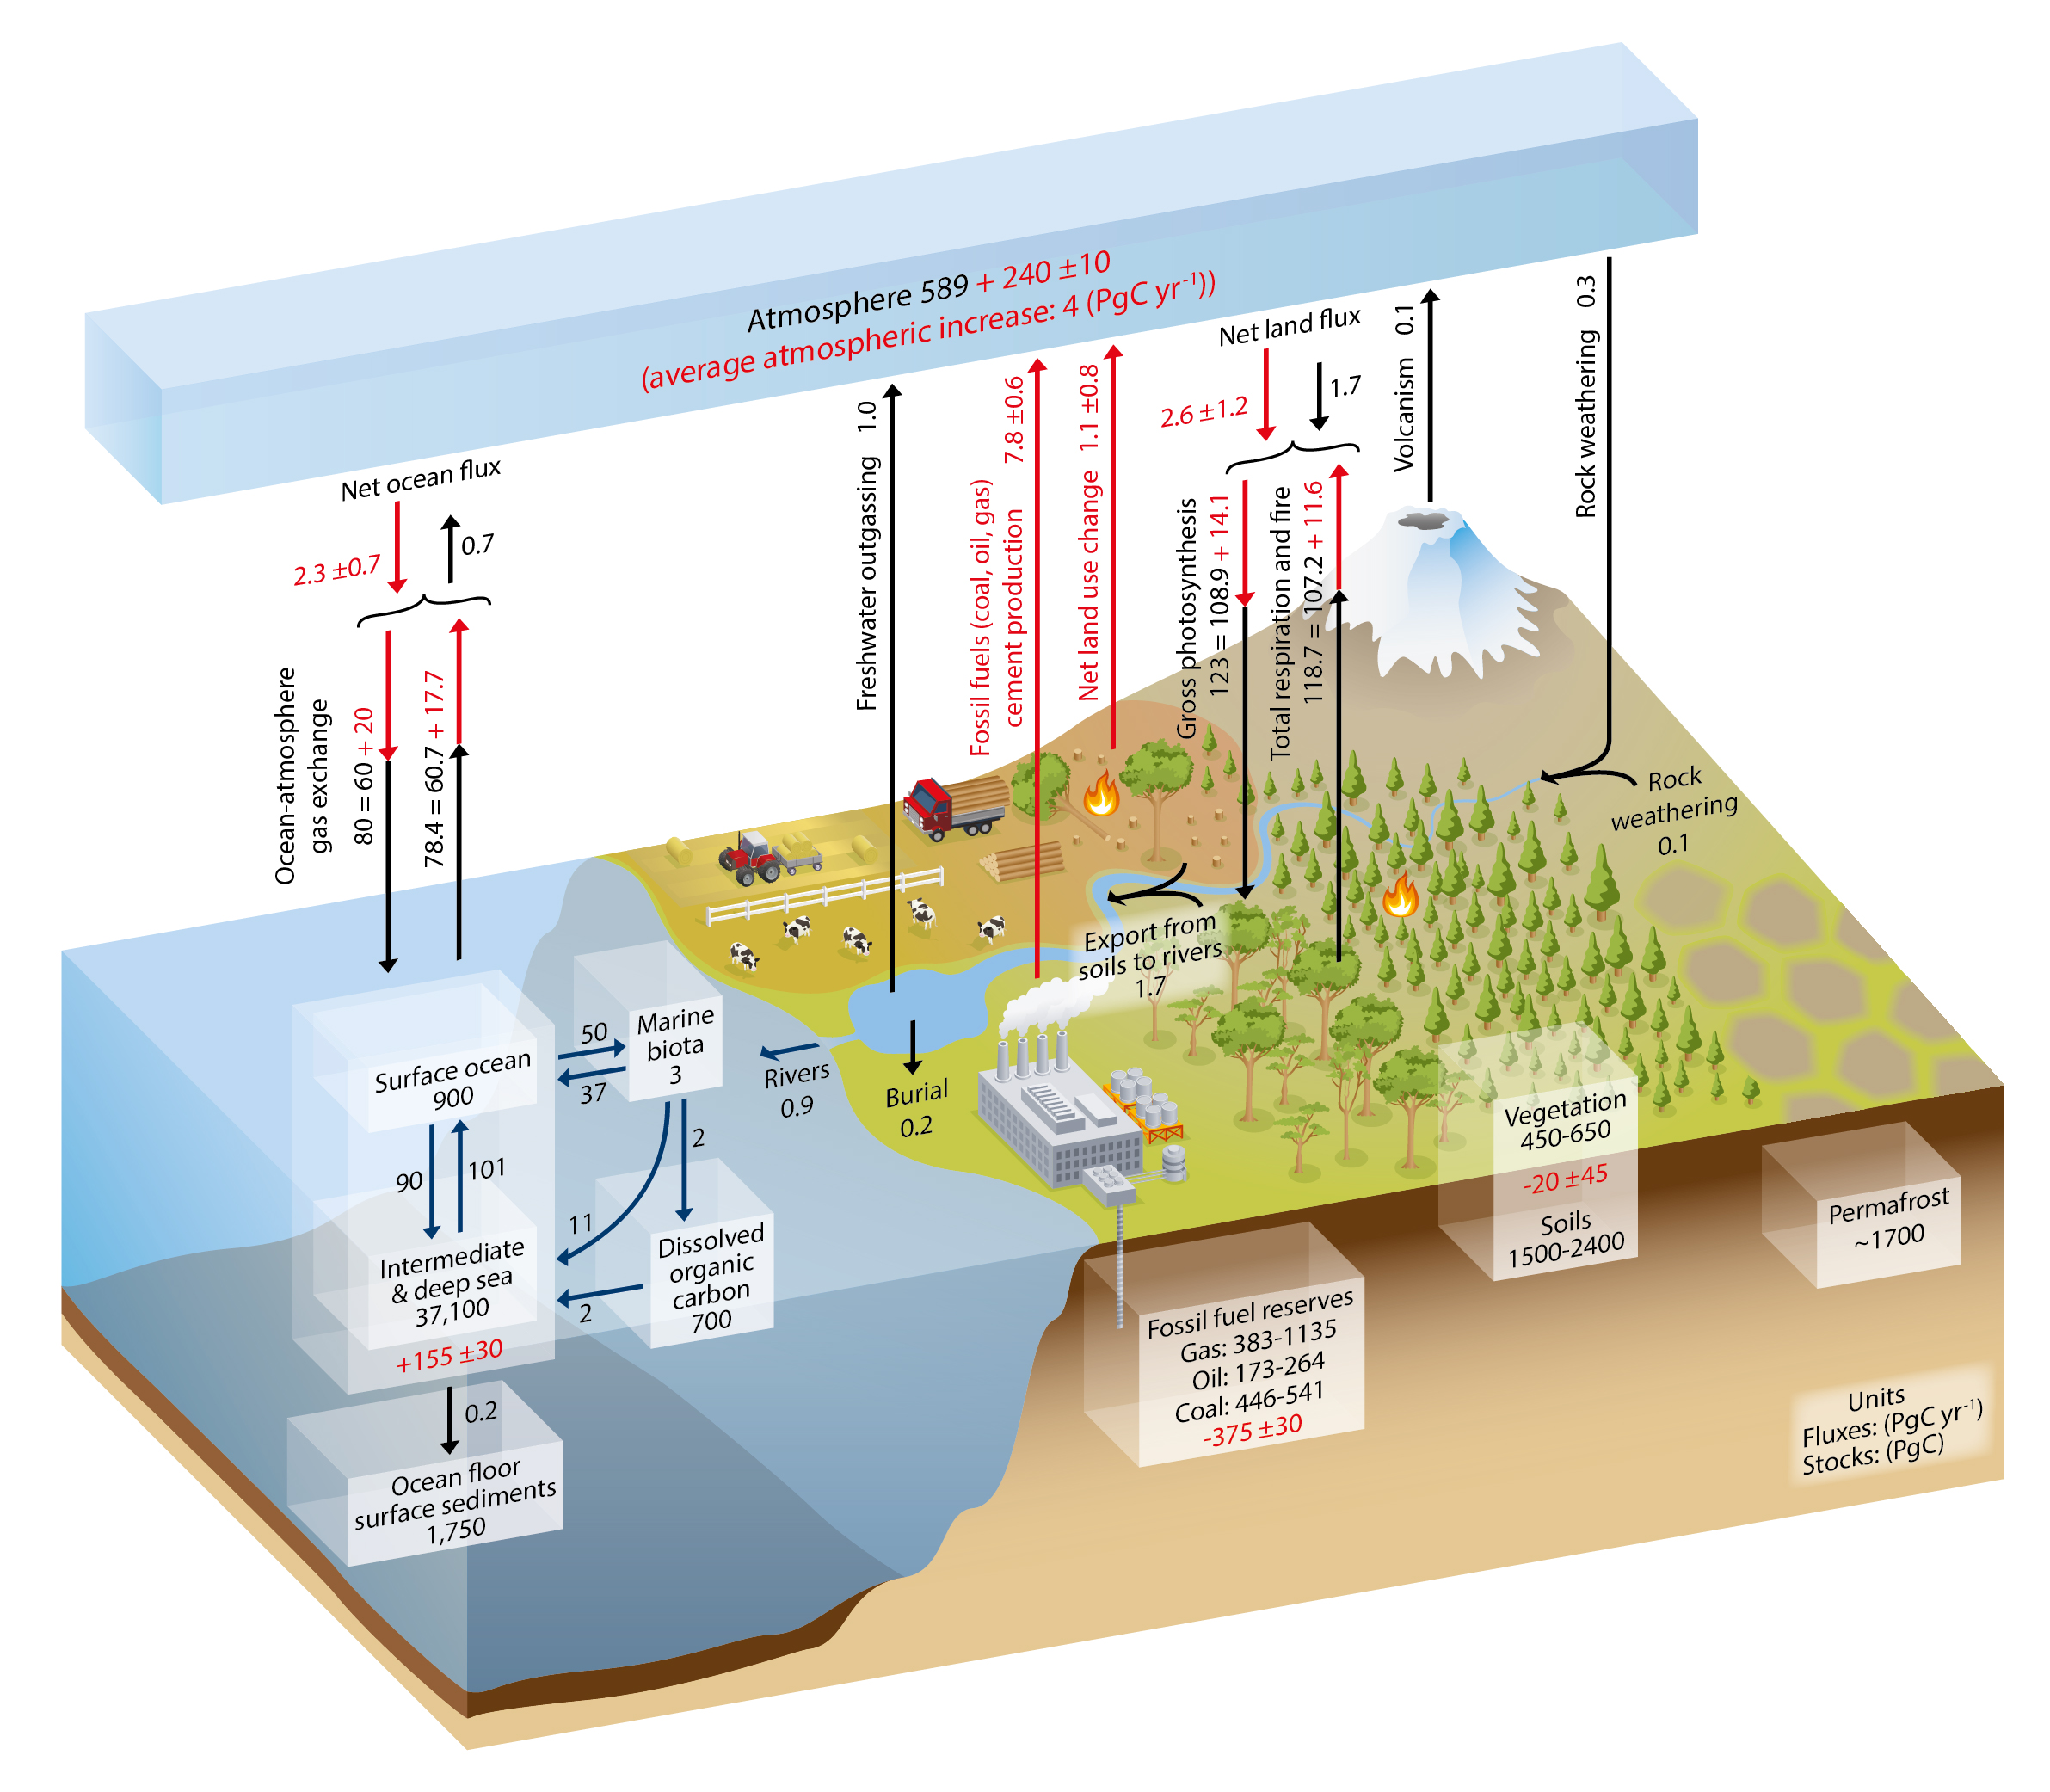
\includegraphics[width=0.9\textwidth]{chapter/chapter1/ipcc_fig6_1.jpg}
    \caption{Global carbon cycle simplified schematic \citep{ciais2014carbon}. Black numbers and arrows represent reservoir mass and exchange fluxes estimated for the time prior to the industrial era (\(\sim\)~1750). Red numbers and arrows represent annual fluxes averaged over the 2000-2009 time period. Red numbers in the reservoirs indicate the cumulative change of carbon over the industrial period (1750-2011).}
    \label{chap1:fig:ipcc_fig6.1}
\end{figure}

As atmospheric CO\(_{2}\) levels have risen, natural sinks of CO\(_{2}\) (fluxes out of the atmosphere) have intensified with both the land surface and oceans absorbing more CO\(_{2}\) from the atmosphere than in pre-industrial times. This can be see in figure~\ref{chap1:fig:ipcc_fig6.1}, with the the net ocean flux of CO\(_{2}\) to the atmosphere decreasing from an estimated +0.7~Pg~C~yr\(^{-1}\) to -2.3~Pg~C~yr\(^{-1}\), and the land surface flux of CO\(_{2}\) to the atmosphere decreasing from -1.7~Pg~C~yr\(^{-1}\) to -2.6~Pg~C~yr\(^{-1}\). More recent estimates from \citet{le2015global} indicate these sinks have further intensified with the ocean sink estimated to be 2.9 \(\pm 0.5\)~Pg~C~yr\(^{-1}\) and the land surface sink 4.1 \(\pm 0.9\)~Pg~C~yr\(^{-1}\) for the year 2014. The intensification of the land carbon sink is thought to be partly due to a combination of forest regrowth as well as rising CO\(_{2}\) and increased nitrogen deposition having a fertilisation effect \citep{ciais2014carbon}. It has also been shown that the land surface sink has been enhanced by an increase in diffuse photosynthetically active radiation as a result of increased cloud cover associated with increased anthropogenic emissions \citep{Mercadodiffuseradiation2009}. 

The partitioning of global carbon fluxes between emissions and sinks is important to better model the carbon cycle. However, current estimates are subject to high levels of uncertainty, which are reflected by the errors shown in Figure~\ref{chap1:fig:ipcc_fig6.1}. Current best estimates of global CO\(_{2}\) emissions and their partitioning between atmospheric growth rate and sinks are shown in Figure~\ref{chap1:fig:ipcc_fig6.8}. It is vitally important to understand the future response of sinks of CO\(_{2}\) (land surface and oceans) to climate change. If either the oceans or land surface were to stop absorbing the same percentage of CO\(_{2}\), we would see even more dramatic increases in atmospheric CO\(_{2}\) levels and thus a much greater rate of global warming. There is a high level of confidence that ocean carbon uptake will continue under all future emission scenarios \citep{ciais2014carbon}. There is much less confidence for the land surface and \citet{1748-9326-7-2-024002} have shown that global warming is particularly sensitive to land surface carbon cycle processes, highlighting the need to improve understanding of land surface carbon uptake. Some estimates show the land surface changing from a sink of CO\(_{2}\) to a source of CO\(_{2}\) under certain future emission scenarios \citep{sitch2008evaluation, cox2000, scholze2006climate}. In the latest IPCC report land surface carbon uptake is still considered the least understood process in the global carbon cycle \citep{ciais2014carbon}.

\begin{figure}[ht]
    \centering
    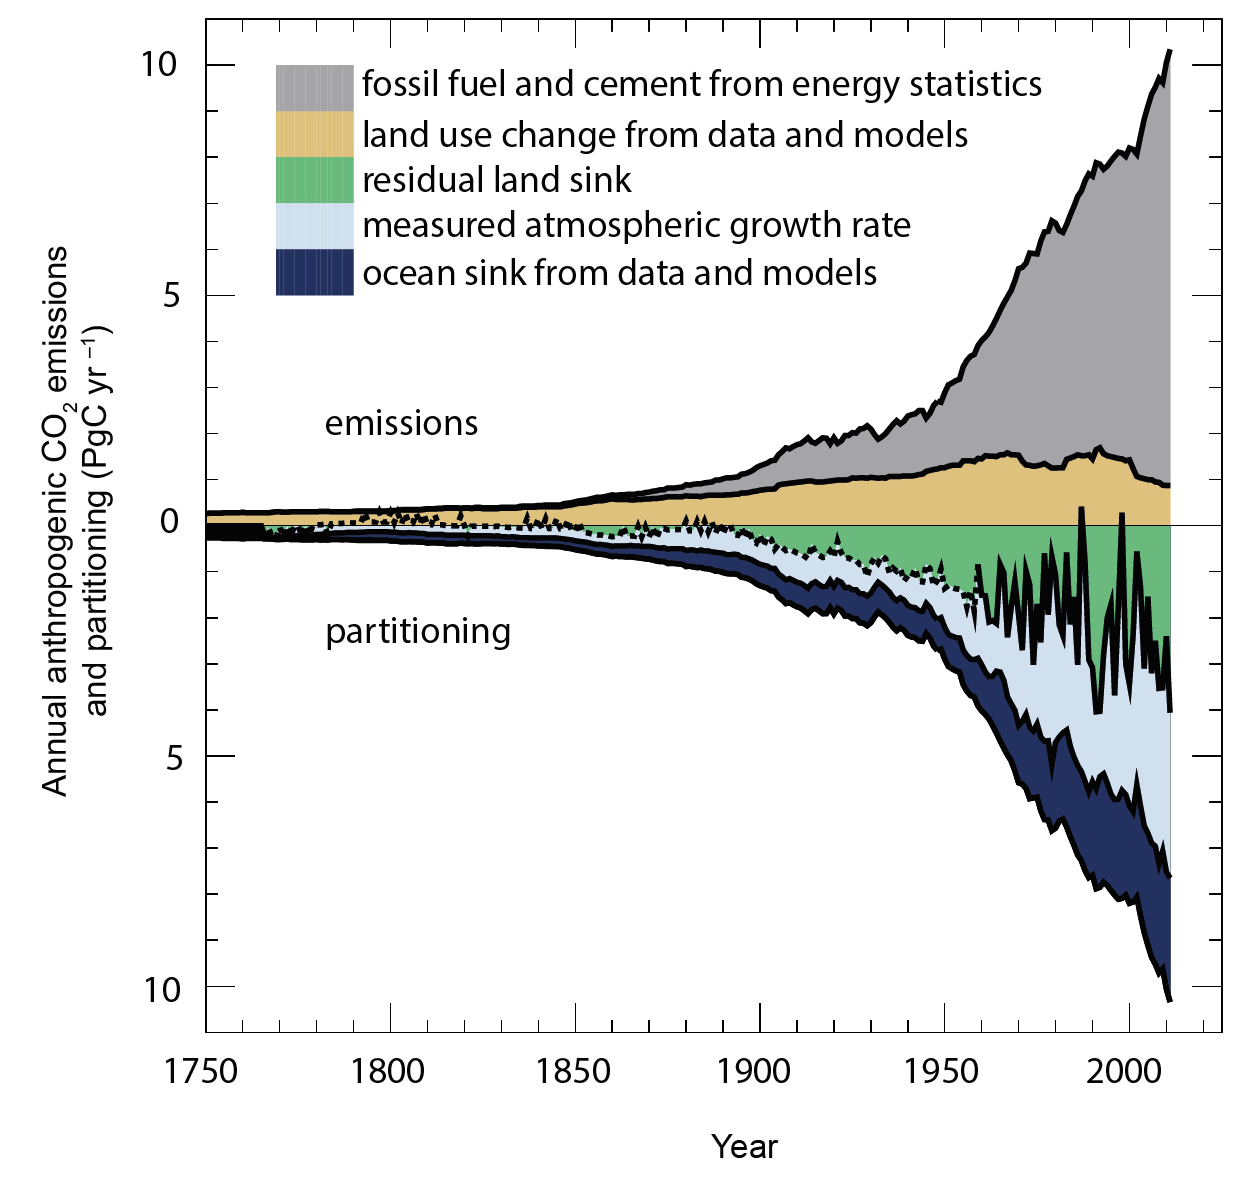
\includegraphics[width=0.9\textwidth]{chapter/chapter1/ipcc_fig6_8.jpg}
    \caption{Annual anthropogenic CO\(_{2}\) emissions and their partitioning among the atmosphere, land and ocean from 1750 to 2011  \citep{ciais2014carbon}.}
    \label{chap1:fig:ipcc_fig6.8}
\end{figure}

Currently land surface carbon uptake is estimated by taking the residual of all other calculated sources and sinks of carbon, so that
\begin{equation}
S_{LAND} = E_{FF} + E_{LUC} - (G_{ATM} + S_{OCEAN})
\end{equation}  
where \(S_{LAND}\) is the global residual land sink of CO\(_{2}\), \(E_{FF}\) is the CO\(_{2}\) emissions from fossil fuels, \(E_{LUC}\) is the CO\(_{2}\) emissions from land use change (mainly deforestation), \(G_{ATM}\) is the atmospheric CO\(_{2}\) growth rate and \(S_{OCEAN}\) is the mean ocean CO\(_{2}\) sink \citep{le2015global}. Figure~\ref{chap1:fig:ipcc_fig6.8} shows the growth in the estimated residual land sink as emissions increase. The high variability shown in this sink is largely due to the fact that it contains the residual errors of the four other terms. However, the land sink also displays some variability due to its sensitivity to year to year variations in precipitation, surface temperature, radiation and volcanic eruptions. Figure~\ref{chap1:fig:ipcc_fig6.8} shows that in 1986 and 1997 the land sink drops to zero, both of these years were among the strongest El Ni\~no's in recent history. In 1997 tropical droughts, often associated with El Ni\~no, were particularly severe leading to wildfires that released vast amounts of stored carbon \citep{schimel2013climate}.

%{\color{red} Include ecosystem flux description and figure here}
Terrestrial ecosystems are made up of autotrophs (organisms capable of photosynthesis) and heterotrophs (organisms that feed on organic carbon). The Gross Primary Productivity (GPP) of an ecosystem is the total amount of carbon removed from the atmosphere by photosynthesis. The Total Ecosystem Respiration (TER) is made up of autotrophic respiration (e.g. from plants) and heterotrophic respiration (e.g. from soil and litter organisms). The total carbon uptake or Net Ecosystem Exchange (NEE) of CO\(_2\) is then equal to -GPP+RT. A representation of these fluxes for a forest ecosystem are shown in Figure~\ref{chap1:fig:eco_fluxes}. 

\begin{figure}[ht]
    \centering
    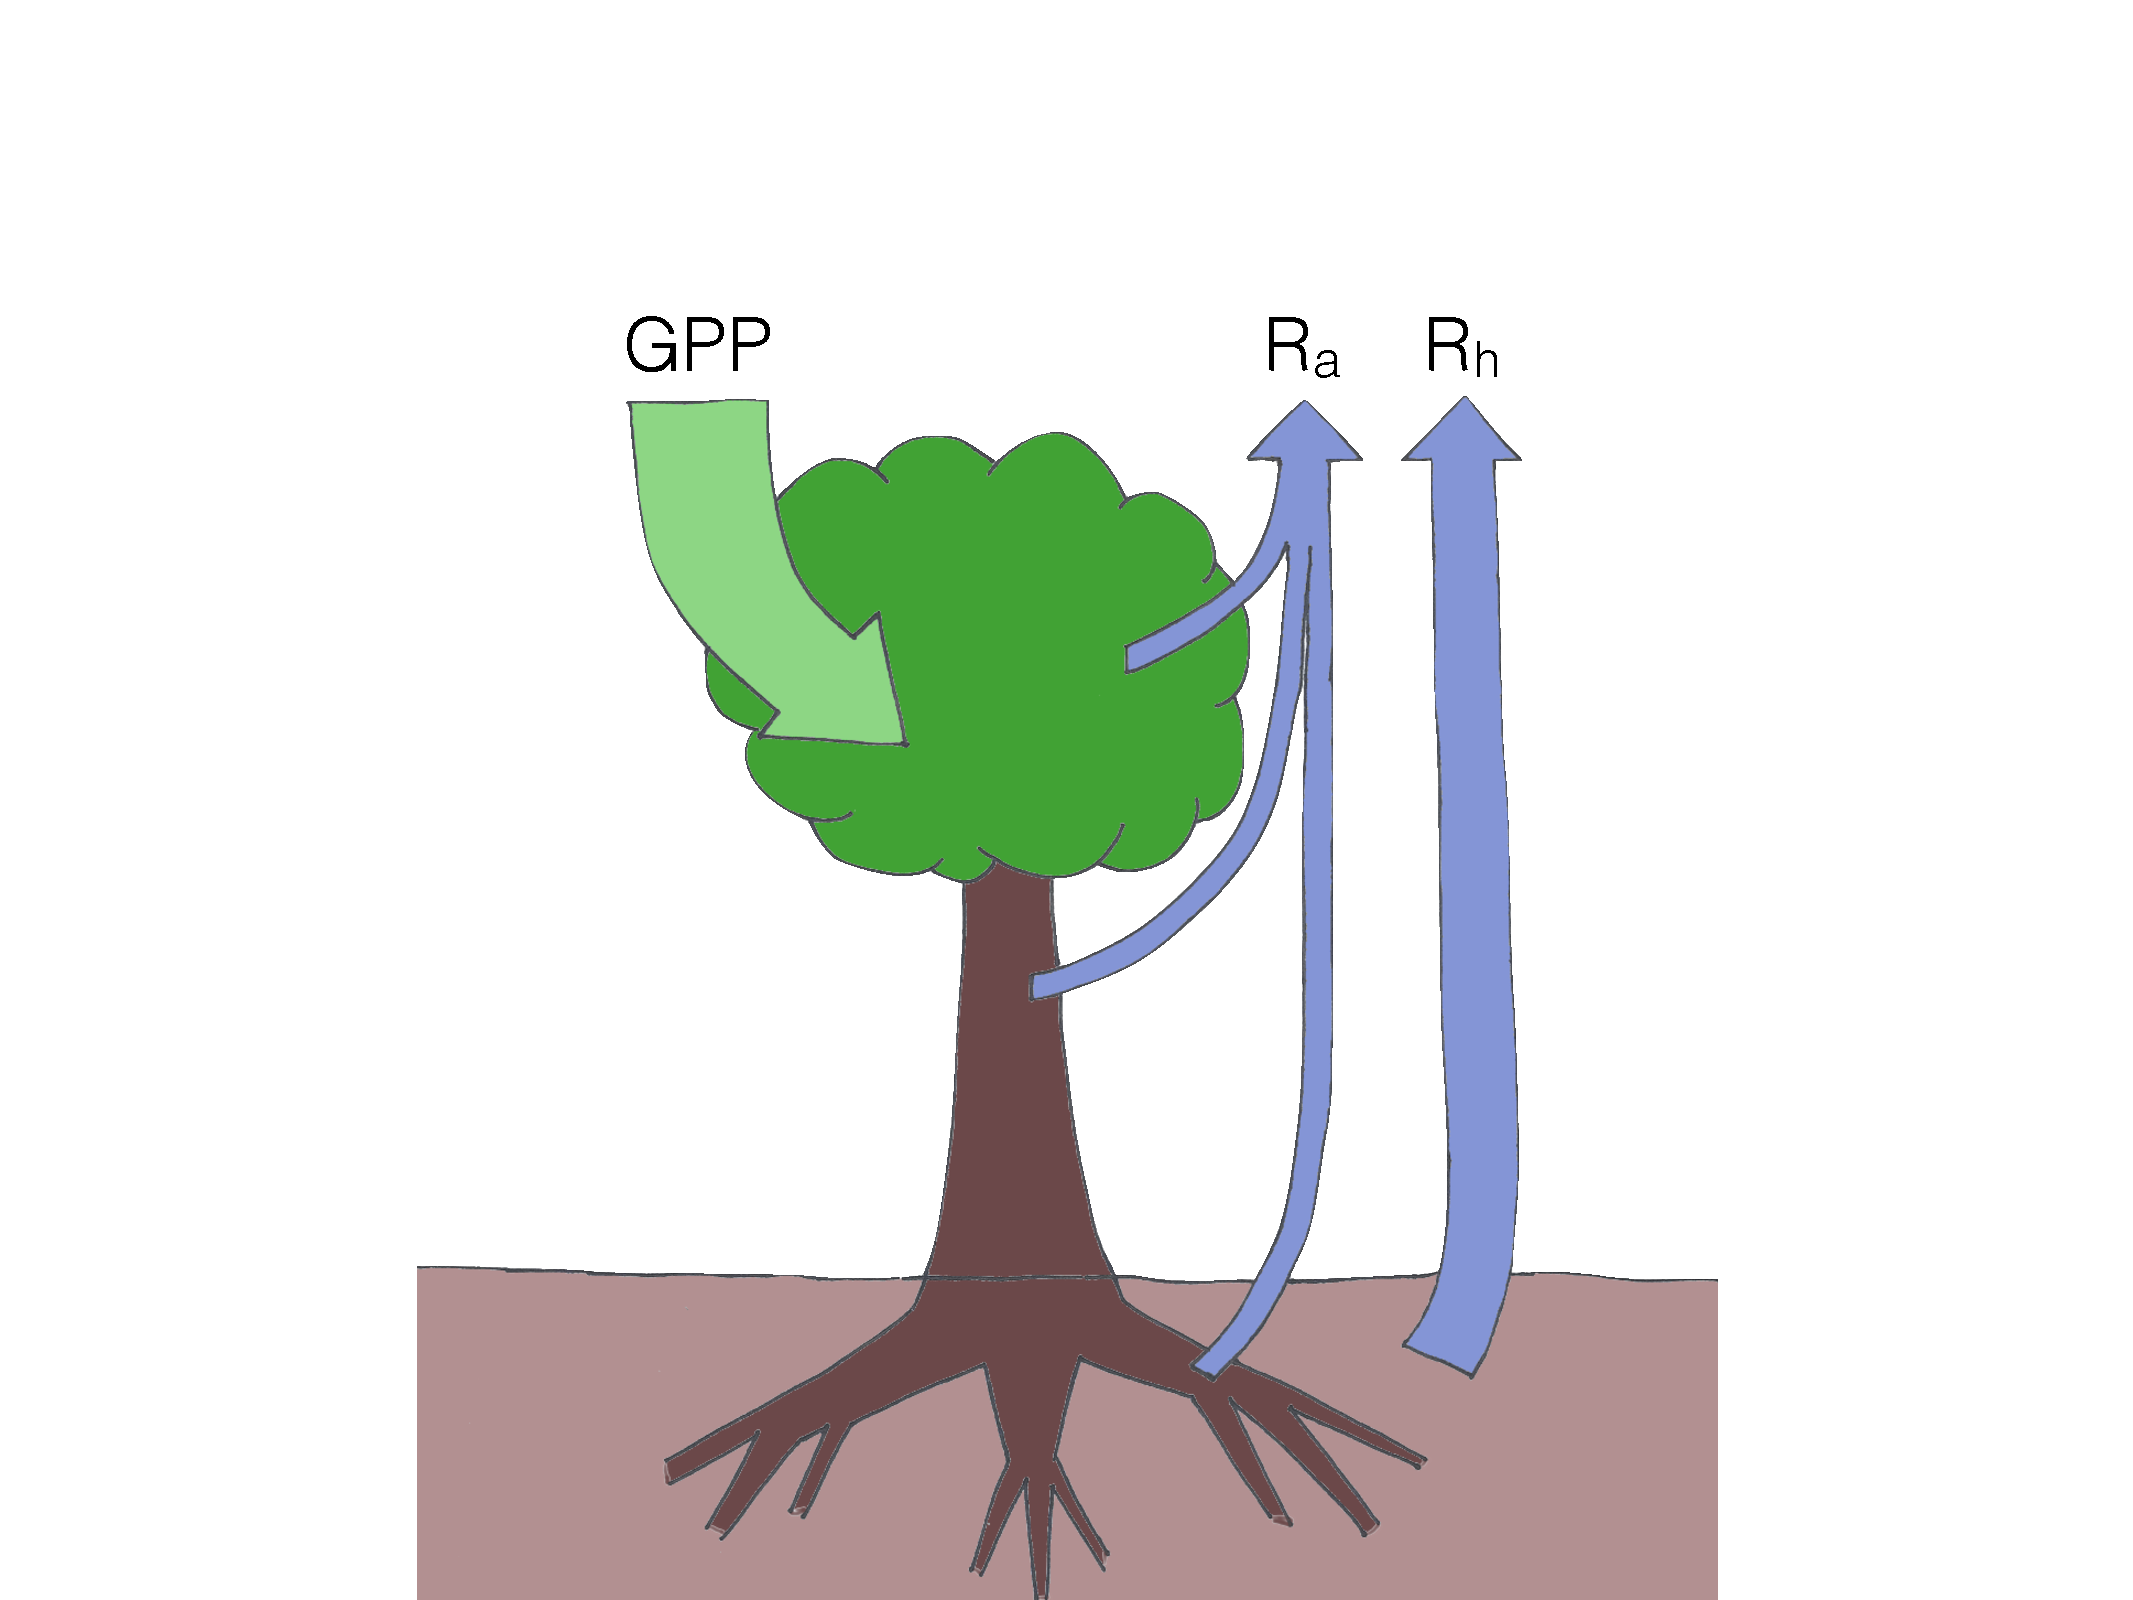
\includegraphics[width=0.5\textwidth]{chapter/chapter1/flux.pdf}
    \caption{Fluxes of carbon through a forest ecosystem. Gross Primary Productivity (GPP) represents total photosynthesis, R\(_{\text{a}}\) is autotrophic respiration from foliage, wood and roots, R\(_{\text{h}}\) is heterotrophic respiration from soil and litter. Total ecosystem respiration of carbon to the atmosphere (RT) is equal to R\(_{\text{a}}\) + R\(_{\text{h}}\). The Net Ecosystem Exchange (NEE) of CO\(_{2}\) is equal to -GPP + RT.}
    \label{chap1:fig:eco_fluxes}
\end{figure}

Disturbance of terrestrial ecosystems from fire, felling and insect outbreak can have significant impacts on carbon dynamics. Land use change is the second largest anthropogenic source of CO\(_{2}\). However, It is not well understood how much CO\(_{2}\) is removed from the atmosphere by regrowth of previously disturbed ecosystems (either by felling or fire), although it is thought that regrowth of forests in partcular could be stronger carbon sinks than their predecessors, due to more rapid biomass accumulation under succession \citep{pan2011large}. Better understanding the response of the land surface to disturbance will help constrain future carbon budgets. 

%Good paper to highlight the fact that the percentage of CO\(_{2}\) absorbed by the land surface has remained approximately constant with rising atmospheric CO\(_{2}\) levels??? Maybe just use IPCC fig 6.8?

%In figure 6.1 and 6.8: Partitioning of fluxes important and hard (shown by error on estimates in fig 6.1). Land surface carbon uptake least understood mechanism in the global carbon cycle, ref IPCC. Will uptake remain the same under climate change.

%Human emissions of CO\(_{2}\) have perturbed the global C cycle and caused a large continual increase in atmospheric CO\(_{2}\) levels.

%Look at papers recommended on Flux Course, some good ones to reference???

%IPCC figure 6.1 and 6.8: Partitioning of fluxes important and hard (shown by error on estimates in fig 6.1). Land surface carbon uptake least understood mechanism in the global carbon cycle, ref IPCC. Will uptake remain the same under climate change.

%\citet{1748-9326-7-2-024002} Have shown that global warming is highly sensitive to land carbon cycle processes and highlighted the need to improve understanding of land surface carbon uptake and its response to climate change. 

\section{Observations of terrestrial carbon balance}

There are an increasing number of available observations relevant to understanding the carbon balance of forests and the terrestrial biosphere. These observations include a range of variables, perhaps two of the most common are the Net Ecosystem Exchange (NEE) of CO\(_{2}\) and Leaf Area Index (LAI), which is the area of leaves per unit area ground. These variables can be directly measured at site level and can also be estimated from satellite remote sensing. Both NEE and LAI are important variables for understanding the carbon balance of ecosystems, with NEE giving us a direct estimate of the carbon uptake of an ecosystem and LAI being a main driver for the amount of GPP an ecosystem can perform.

%para on flux network and site level data:
At site level, flux towers measuring ecosystem-atmosphere fluxes of CO\(_{2}\), water and energy using the micrometeorological technique of eddy covariance provide one of the most valuable sources of information. Direct observations of ecosystem CO\(_{2}\) uptake are made at a fine temporal resolution, with observations every half-hour. A global flux network (FLUXNET), was established in 1997 \citep{baldocchi2001fluxnet}, to consolidate the information from a growing number of flux tower sites. Currently there are 517 active FLUXNET sites which are shown in Figure~\ref{chap1:fig:fluxnet_2015}, as can be seen these sites are not uniformly distributed so it is not possible to use FLUXNET sites alone to produce global estimates of terrestrial CO\(_{2}\) balance. However, these sites do provide an invaluable resource for model and satellite calibration. In turn this can be used to produce estimates on a global scale. At many flux tower sites and forest stands other diverse observations relevant to terrestrial carbon budgets are also being made. These include observations of soil and litter respiration, woody biomass and LAI. However, because they are labour intensive these observations are made much less frequently.     

\begin{figure}[ht]
\centering
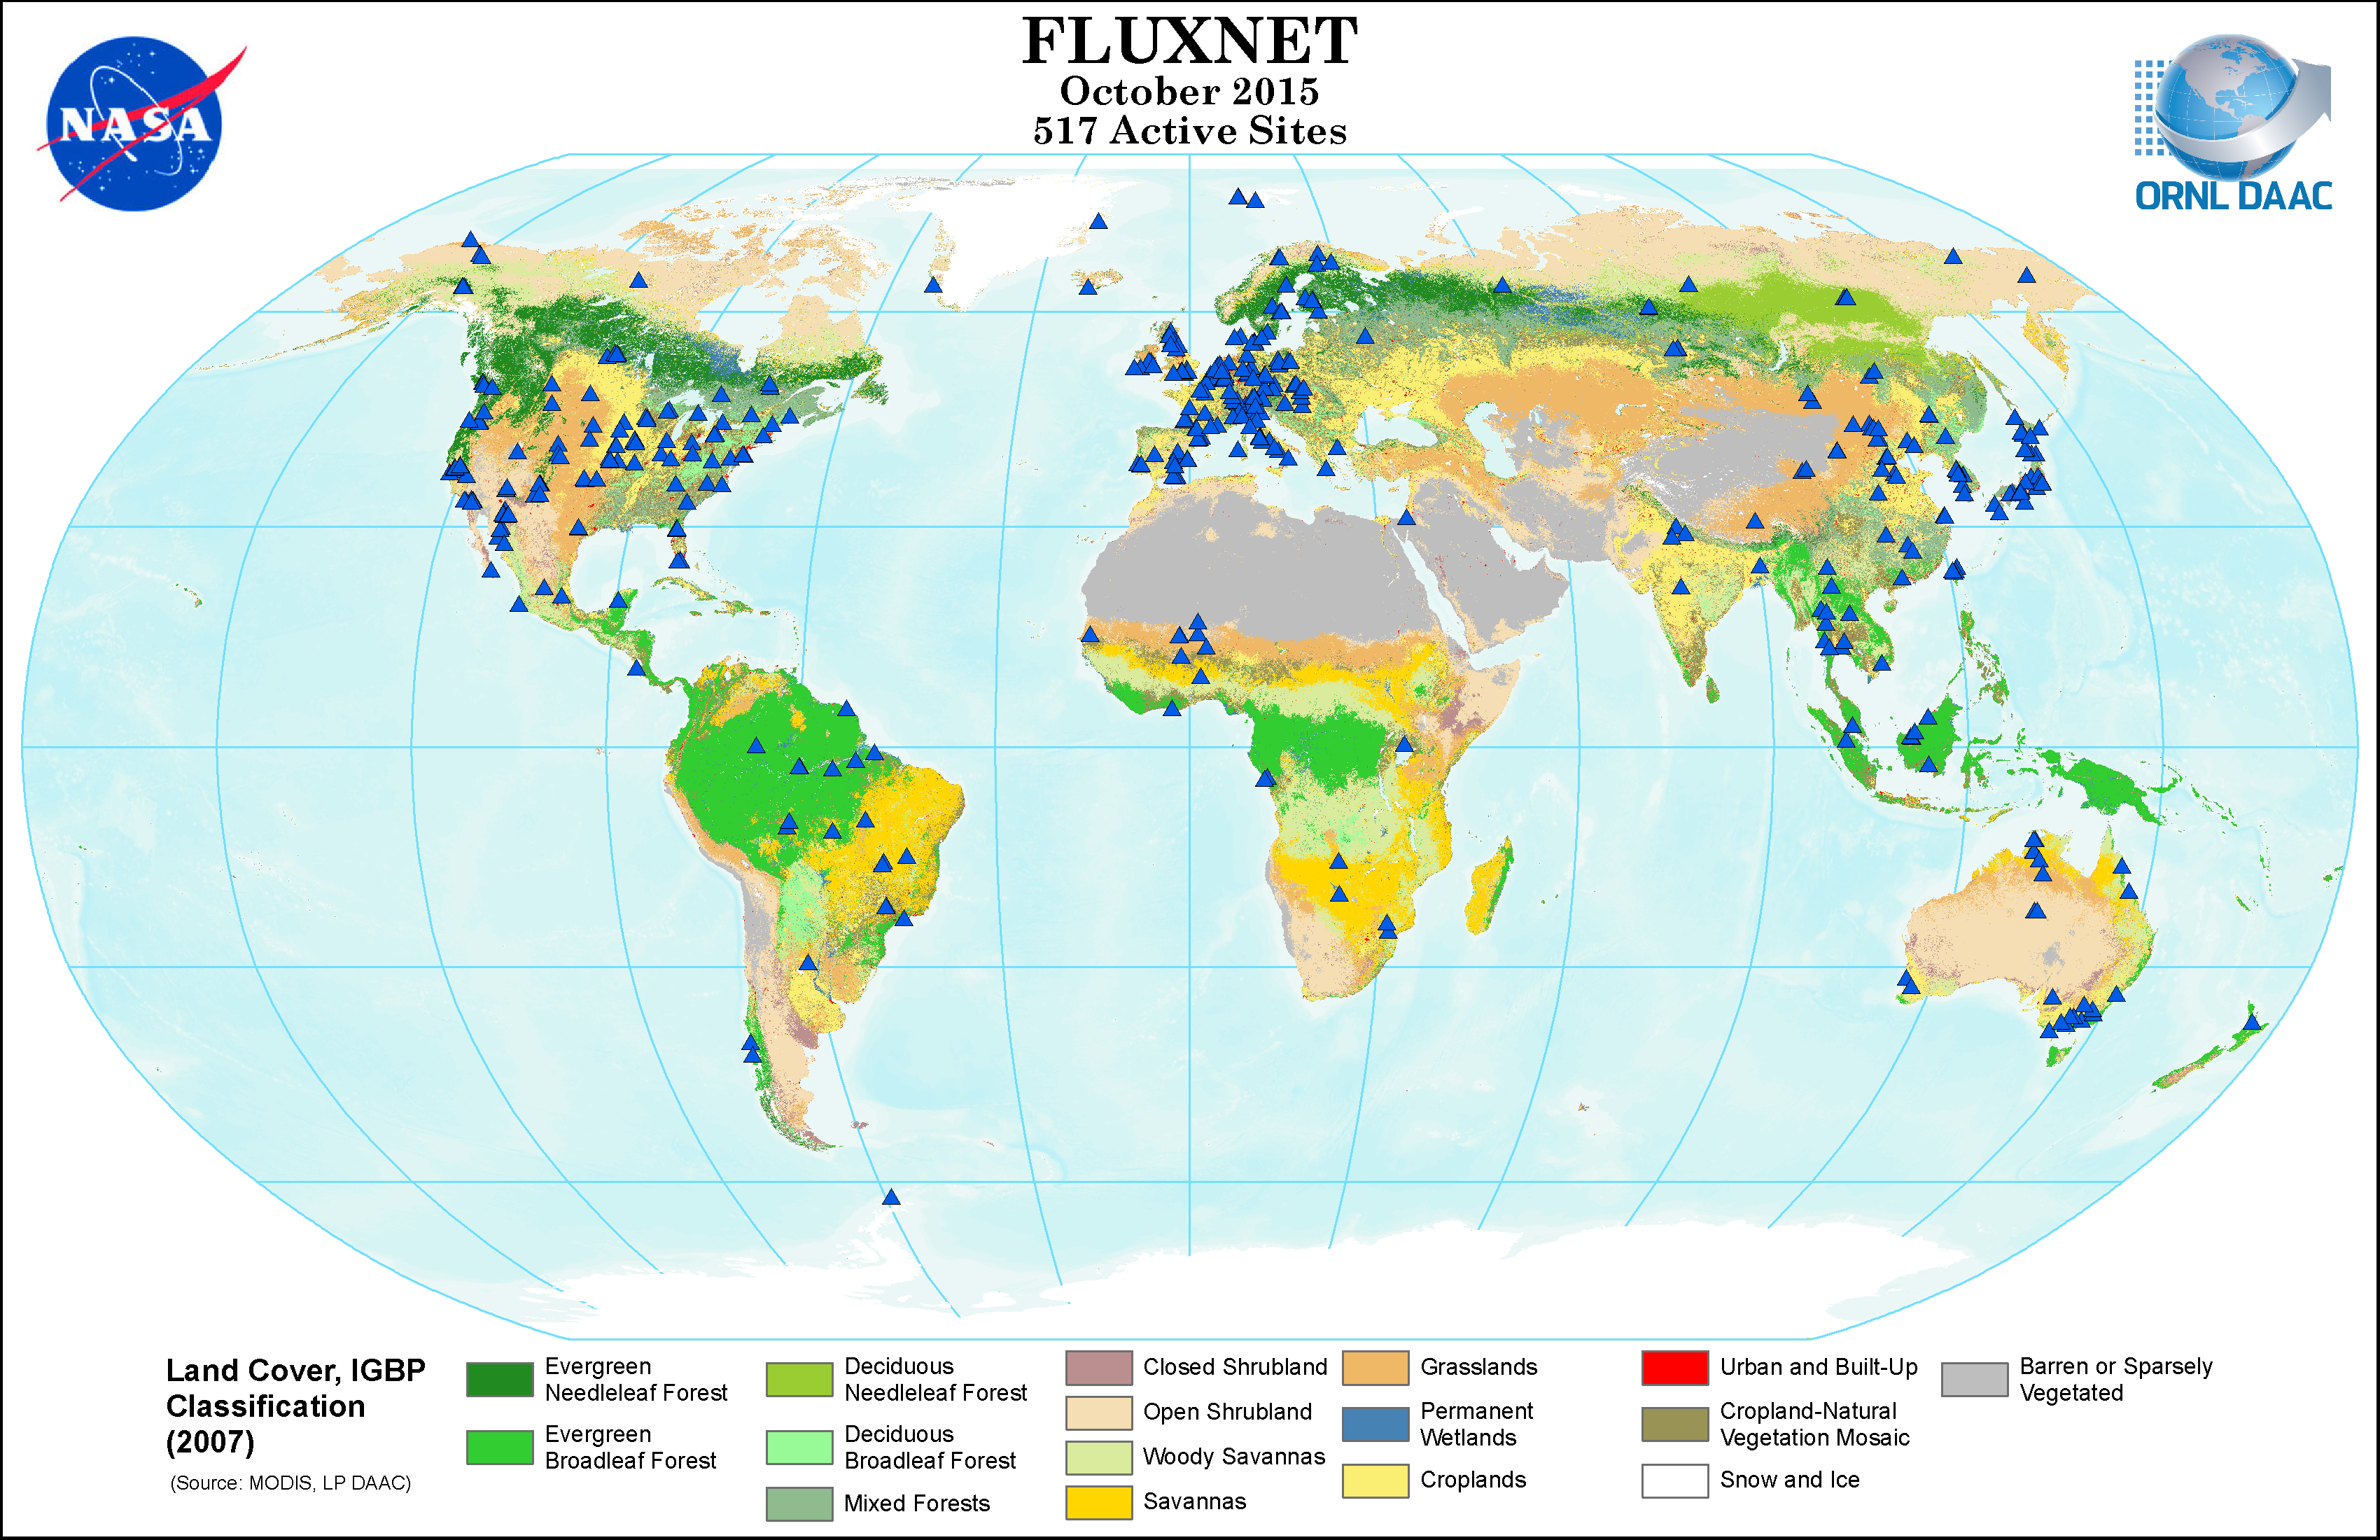
\includegraphics[width=0.9\textwidth]{chapter/chapter1/FluxNetworkMODIS_IGBP_10-2015.png}
\caption{FLUXNET sites and land cover (MODIS IGBP classification) \citep{fluxnetsite2013}.}
\label{chap1:fig:fluxnet_2015}
\end{figure}

%para on satellite data
The Moderate Resolution Imaging Spectroradiometer (MODIS) on the TERRA and AQUA satellites produces global estimates of LAI and Gross Primary Productivity (GPP) for terrestrial ecosystems \citep{running2004continuous}. However, MODIS actually measures reflected sunlight, this is then converted to vegetation indices, such as the Normalised Difference Vegetation Index (NDVI). These indices are correlated with the fraction of absorbed visible sunlight to estimate LAI or used in simple algorithms to estimate GPP \citep{yuan2007deriving}. It is therefore important to understand the limitations when interpreting satellite products as they do not represent direct observations. For LAI it has been shown that remotely sensed estimates saturate when measuring ecosystems with a LAI above 3 \citep{myneni2002global}. Terrestrial fluxes of carbon estimated from satellite measurements are subject to large errors in representativity, as satellites view a scene almost instantaneously and then derive daily mean fluxes \citep{baldocchi2008turner}. 
%Baldocchi paper: Many observations of forest carbon flux made worldwide.

\section{The role of models}

Observations can only tell us about the current and past state of a system. In order to produce future predictions and better understand current terrestrial carbon dynamics we must use mathematical models. Figure~\ref{chap1:fig:ipcc_fig6.16} show a comparison of the residual land sink (described in section~\ref{chap1:sec:global_c_cycle}) with the global terrestrial CO\(_{2}\) sink estimated from different process based global carbon cycle models. We see that although there is a high variability between modelled estimates there is good agreement between the multi-model mean and the residual land sink. 

\begin{figure}[ht]
    \centering
    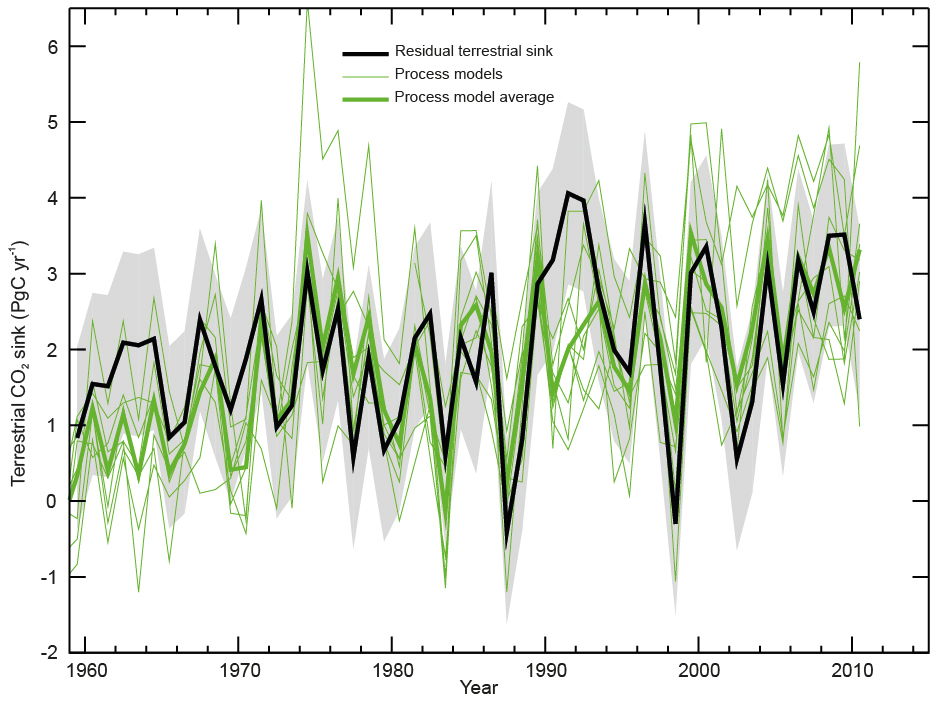
\includegraphics[width=0.9\textwidth]{chapter/chapter1/ipcc_fig6_16.jpg}
    \caption{Comparison of the residual land sink (black line) with the global terrestrial CO\(_{2}\) sink estimated from different process based global carbon cycle models \citep{ciais2014carbon}. Grey shading represents uncertainty in residual land sink.}
    \label{chap1:fig:ipcc_fig6.16}
\end{figure}

Representative Concentration Pathways (RCPs) of CO\(_{2}\) concentrations and emissions have been developed \citep{moss2010next} to drive climate models to produce future predictions. Under these pathways land surface carbon uptake is highly uncertain with little agreement between different process based models. Some predict the land surface to become a source of CO\(_{2}\) and others predict a further intensification of the residual land sink \citep{jones2013twenty}. This large uncertainty for land surface models is partly due to poor model parameterisations and missing processes within models. One of the main processes many current global models do not account for is the effect of disturbance on terrestrial ecosystem carbon dynamics.

It has been shown that many terrestrial carbon cycle models simulating the seasonal cycle of land-atmosphere CO\(_{2}\) exchange perform poorly when compared to FLUXNET sites in North America \citep{schwalm2010model}. Here a difference between observations and model predictions of 10 times the observational uncertainty was found, highlighting the need for continued model development. In order to improve global models of terrestrial carbon balance it is important to use site-level-research to hone the processes and parameterisations of the models where we have diverse sets of direct observations with which to judge modified-model performance. 
%IPCC figure 6.16 and section 6.3.2.6.6: Contribution of models to understanding the terrestrial carbon cycle. Reference every DALEC paper.


\section{Data assimilation}

%{\color{red} Observations are sparse, current model predictions are poor, data assimilation provides a way to combine both sources of information to improve current estimates.}

As discussed above, the level of uncertainty in terrestrial carbon balance predictions arise from significant gaps in the direct observations available and from a lack of clarity and authoritative parameterisation of the constituent processes in current models. The technique of data assimilation provides a method for combining and comparing the output of predictive models with incomplete observations to find the best estimate for the state and parameters of a system. Data assimilation has had many successful applications. Perhaps the most important application has been in numerical weather prediction where data assimilation has contributed to forecast accuracy being increased at longer lead times, with the result that the four day forecast in 2014 now has the same level of accuracy as the one day forecast in 1979 \citep{bauer2015quiet}. Obviously, this improved forecasting is not solely due to data assimilation but also increased quality and resolution of observations along with improvements in model structure, however the introduction and evolution of data assimilation has been a key part of the improvement \citep{dee2011era}.

More recently data assimilation has been used to improve our knowledge of ecological systems. For the carbon balance of forests it has been used to combine many different observations with functional ecology models \citep{zobitz2011primer, fox2009reflex, richardson2010estimating, Quaife2008, Zobitz2014, Niu2014}. Global land surface models have also been implemented with data assimilation, mainly using data from satellite and atmospheric $\text{CO}_{2}$ observations \citep{Kaminski2013, scholze2007propagating}. In a few cases site level data has also been assimilated \citep{Verbeeck2011, Bacour2015}. In comparison with numerical weather prediction, the use of data assimilation in these areas is relatively new and underdeveloped. The further application of data assimilation to models of ecosystem carbon balance will help to improve model parameterisations and future predictions. The development of improved data assimilation techniques will also help to  identify missing model processes and changes in model parameters and behaviour over time. In particular, understanding the change in model parameters over time will be of use in improving models predictions of the effect of disturbance in terrestrial ecosystems.
  
%Role of DA in NWP improving forecast skill. 



\chapter{Thesis aims and outline}
\label{chap:aims}
%Thesis aims and outline

The primary aim of this thesis is the development of data assimilation techniques for the terrestrial carbon cycle, in order to aid progress in this field of research. We focus on implementing novel data assimilation methods with a simple model of ecosystem carbon balance in order to address three key areas:

\begin{enumerate}
\item \textit{Investigating the information content in distinct carbon balance observations for data assimilation}

It is important to understand which observations provide most information to data assimilation schemes. We investigate the different relative levels of information for observations relevant to ecosystem carbon balance through novel applications of information content metrics.

\item \textit{Improving the representation of prior and observational errors in carbon cycle data assimilation}

Currently the specification of both prior and observational errors for the carbon cycle has been simplistic. We seek to improve this representation by investigating the role of correlations between errors for both prior estimates and observations. We judge the effect of including these error correlations on data assimilation results.
  
\item \textit{Using data assimilation to understand the effect of disturbance on forest carbon dynamics}

The effect of disturbance (e.g. fire, felling, insect outbreak) on ecosystem carbon dynamics is one of the least understood components of the global carbon cycle. We investigate the effect of selective felling on forest carbon uptake using novel data assimilation techniques.
\end{enumerate}

From this point onwards the thesis is structured as follows:

\begin{itemize}
\item \textbf{Chapter~\ref{chap:litrev}} introduces the concept of data assimilation and relevant methods. In particular applications of data assimilation to the terrestrial carbon cycle are discussed. We highlight some of the current issues faced and areas for future development.  

\item \textbf{Chapter~\ref{chap:data}} provides an explanation of the Data Assimilation Linked Ecosystem Carbon (DALEC and DALEC2) models used throughout the thesis. The fieldwork campaign conducted during this PhD project is outlined along with additional flux tower data from the Alice Holt research site (Hampshire, UK).

\item \textbf{Chapter~\ref{chap:info_con}} explores the first aim of the thesis. The DALEC and DALEC2 model are are used in a set of information content experiments, with novel applications of information content metrics, in order to better understand the relative levels of information from different observations and how information content might vary in time and with different characterisations of errors.

\item \textbf{Chapter~\ref{chap:error_corrs}} addresses the second aim of the thesis. The role of prior and observation error correlations are investigated in a set of data assimilation experiments to understand their contribution to improving a model forecast of forest carbon uptake.

\item \textbf{Chapter~\ref{chap:disturbance}} 
\end{itemize}
     
%Figure Example:

%\begin{figure}[htbp]
%\centering
%\includegraphics[trim=5pc 20pc 5pc 20pc, clip=true, width=0.8\textwidth]{chapter/chapter2/ch2fig1}
%\caption{\small Annual anomalies of global land-surface air temperature ($^\circ$C), 1850 to 2005 from several datasets. The smooth curves show decadal variations. Figure 3.1 from Climate Change 2007: The Physical Science Basis. Contribution of Working Group I to the Fourth Assessment Report of the Intergovernmental Panel on Climate Change.}
%\label{ch2fig1}
%\end{figure}


\chapter{Current state of data assimilation for the carbon cycle}
\label{chap:litrev}
%Chapter 3


\section{Data assimilation methods}

Data assimilation provides techniques for combining observations and prior knowledge of a system in an optimal way to find an improved estimate of the system. The prior knowledge of a system often takes the form of a numerical model and an initial guess of the model state/parameters. Many statistical methods have been developed for data assimilation. These methods can largely be categorised as either sequential or variational. Sequential algorithms solve the system of equations needed to find an optimal solution explicitly at each observation time. Variational methods solve the equations needed for an optimal solution implicitly by minimising a cost function for all available observations over some time window. This thesis is mainly concerned with the variational technique of four-dimensional variational data assimilation (4D-Var). 

In numerical weather prediction data assimilation has been predominately used for state estimation whilst keeping parameters fixed. This is because numerical weather prediction is mainly dependent on the initial state with model physics being well understood. Ecosystem carbon cycle models are more dependent on finding the correct set of parameters to describe the ecosystem of interest \citep{luo2015predictability}. We therefore discuss data assimilation for joint state and parameter estimation. In the next sections (\ref{sec:intro_da} to \ref{sec:mcmc_seq}) we give a general introduction to data assimilation, then expand this to 4D-Var and finally we briefly discuss other data assimilation methods not directly used in this thesis but applicable to subsequent discussion. 

\subsection{Introduction to data assimilation} \label{sec:intro_da}

We consider a system that can be described by a numerical model with a true model state \(\textbf{z}^{t} \in \mathbb{R}^{n}\) and true parameters \(\textbf{p}^{t} \in \mathbb{R}^{q}\). We then define the true augmented state as
\begin{equation}
\textbf{x}^{t} =
\begin{pmatrix}
\textbf{p}^{t} \\
\textbf{z}^{t}
\end{pmatrix}
\in \mathbb{R}^{q+n}.
\end{equation}
The initial guess to this model augmented state \(\textbf{x}^{b} \in \mathbb{R}^{q+n}\) (often referred to as the prior or background) and observations of the system \(\textbf{y} \in \mathbb{R}^{m}\) will only be approximations to the true system state, such that
\begin{equation}
\textbf{x}^{b} = \textbf{x}^{t} + \bm{\epsilon}^{b}, \label{eqn:xb}
\end{equation} 
\begin{equation}
\textbf{y} = h(\textbf{x}^{t}) + \bm{\epsilon}^{o}, \label{eqn:y}
\end{equation} 
where \( \bm{\epsilon}^{b}\) and \( \bm{\epsilon}^{o}\) are the prior and observation errors respectively, and \(h: \mathbb{R}^{q+n}\rightarrow \mathbb{R}^{m}\) is the observation operator (can be linear or non-linear) mapping the augmented state to the observations. The errors in the prior and observations are assumed to be unbiased and mutually independent with known covariance matrices \(\textbf{B} = \mathbb{E}[\bm{\epsilon}^{b}(\bm{\epsilon}^{b})^{T}]\) and \(\textbf{R} = \mathbb{E}[\bm{\epsilon}^{o}(\bm{\epsilon}^{o})^{T}]\).

The best estimate to \(\textbf{x}^{t}\) satisfying both equation~\eqref{eqn:xb} and \eqref{eqn:y} is often called the analysis or the posterior estimate, here denoted \(\textbf{x}^{a}\). It is possible to derive this analysis by applying Bayesian methods to probability density functions. Bayes' theorem, first discussed in \citet{bayes1763} but formalised by \citet{laplace1781memoire}, states that the posterior probability of event A given that event B occurs, is proportional to the prior probability of A multiplied by the probability of event B given that event A occurs, this can be expressed mathematically as
\begin{equation}
\mathbb{P}(A|B) \propto \mathbb{P}(A)\mathbb{P}(B|A). \label{eqn:bayes}
\end{equation}
For data assimilation event A represents the augmented state of the system \(\textbf{x}\) and event B the observations \(\textbf{y}\). Maximising the probability \(\mathbb{P}(A|B)\) is then equivalent to finding the augmented state that best represents the observations. 

If we make the assumption of Gaussian probability density functions with
\begin{equation}
\mathbb{P}^{b}(\textbf{x}) = \frac{1}{\sqrt{|2\pi\textbf{B}|}}\text{exp}\big(-\frac{1}{2}(\textbf{x}-\textbf{x}^{b})^{T}\textbf{B}^{-1}(\textbf{x}-\textbf{x}^{b})\big)
\end{equation}
and
\begin{equation}
\mathbb{P}^{o}(\textbf{y}|\textbf{x}) = \frac{1}{\sqrt{|2\pi\textbf{R}|}}\text{exp}\big(-\frac{1}{2}(\textbf{y}-h(\textbf{x}))^{T}\textbf{R}^{-1}(\textbf{y}-h(\textbf{x}))\big),
\end{equation}
where \(\mathbb{P}^{b}(\textbf{x})\) is the probability density function for the prior and \(\mathbb{P}^{o}(\textbf{y}|\textbf{x})\) the probability density function of the observations given the augmented state. Then from Bayes' theorem (equation~\eqref{eqn:bayes}) the posterior probability density function for the augmented state
\begin{equation}
\begin{split}
\mathbb{P}^{a}(\textbf{x}|\textbf{y}) &\propto \frac{1}{\sqrt{|2\pi\textbf{B}|}\sqrt{|2\pi\textbf{R}|}}\text{exp}\big(-\frac{1}{2}(\textbf{x}-\textbf{x}^{b})^{T}\textbf{B}^{-1}(\textbf{x}-\textbf{x}^{b})-\frac{1}{2}(\textbf{y}-h(\textbf{x}))^{T}\textbf{R}^{-1}(\textbf{y}-h(\textbf{x}))\big) \\
&\propto \text{exp}\big(-\frac{1}{2}(\textbf{x}-\textbf{x}^{b})^{T}\textbf{B}^{-1}(\textbf{x}-\textbf{x}^{b})-\frac{1}{2}(\textbf{y}-h(\textbf{x}))^{T}\textbf{R}^{-1}(\textbf{y}-h(\textbf{x}))\big), \label{eqn:p_x_y}
\end{split}
\end{equation} 
here we can ignore the constant multiplying the exponential function as it is independent of \textbf{x}. We want to maximise the probability of the augmented state \textbf{x} given the observations \textbf{y}, from equation~\eqref{eqn:p_x_y} we can see that to maximise \(\mathbb{P}^{a}(\textbf{x}|\textbf{y})\) we must maximise the terms in the exponent, this is equivalent to minimising the quadratic cost function 
\begin{equation}
J(\textbf{x}) = \frac{1}{2}(\textbf{x}-\textbf{x}^{b})^{T}\textbf{B}^{-1}(\textbf{x}-\textbf{x}^{b}) + \frac{1}{2}(\textbf{y}-h(\textbf{x}))^{T}\textbf{R}^{-1}(\textbf{y}-h(\textbf{x})). \label{eqn:3dvar}
\end{equation}
This is the cost function minimised in three-dimensional variational data assimilation (3D-Var), where the minimum is found using a descent algorithm evaluating equation~\eqref{eqn:3dvar} and its gradient \citep{courtier1998ecmwf}. We can approximate the minimum of \eqref{eqn:3dvar} by finding its gradient and setting it to zero to obtain the Best Linear Unbiased Estimate (BLUE) \citep{talagrand1997assimilation} where
\begin{equation}
\textbf{x}^{a} = \textbf{x}^{b} + \textbf{K}(\textbf{y} - h(\textbf{x}^{b})), \label{eqn:blue}
\end{equation}
\begin{equation}
\textbf{K} = \textbf{B}\textbf{H}^{T}(\textbf{H}\textbf{B}\textbf{H}^{T}+\textbf{R})^{-1},
\end{equation}
where \textbf{K} is the Kalman gain matrix specifying the weight of the analysis increment and \(\textbf{H}=\frac{\partial h(\textbf{x})}{\partial \textbf{x}}\) is the linearised observation operator. We can also approximate the analysis error covariance matrix as
\begin{equation}
\textbf{A} = (\textbf{H}^{T}\textbf{R}^{-1}\textbf{H}+\textbf{B}^{-1})^{-1}, \label{eqn:a_cov}
\end{equation}
if \( h \) is linear then \eqref{eqn:blue} and \eqref{eqn:a_cov} are exact solutions.
%(BLUE) introduce basic concept of DA for a linear Gaussian time-invariant system... will use this in Info Con chapter

%BLUE \(\rightarrow\) 3D-Var

\subsection{4D-Var}

%*Brief* but inclusive of all notation need for results chapter on information content
4D-Var extends 3D-Var to allow for the assimilation of observations distributed throughout some time interval \(t_{0}\) to \(t_{N}\). \citet{Sasaki70somebasic} proposed a method for combining a time series of observations with a numerical model, which was then further developed for use in numerical weather prediction \citep{dimet1986variational}. In 4D-Var we minimise the cost function,

\begin{equation}
J(\textbf{x}_0) = \frac{1}{2}(\textbf{x}_0-\textbf{x}^b)^{T}\textbf{B}^{-1}(\textbf{x}_0-\textbf{x}^b)+\frac{1}{2}\sum_{i=0}^{N}(\textbf{y}_i-\textbf{h}_i(\textbf{x}_i))^{T}\textbf{R}_{i}^{-1}(\textbf{y}_i-\textbf{h}_i(\textbf{x}_i)), \label{eqn:4dvar_cost}
\end{equation}

to obtain the analysis \(\textbf{x}^{a}_{0}\), valid at the initial time \(t_{0}\), subject to the strong constraint that the model states (\(\textbf{x}_0, \dots, \textbf{x}_N\)) must satisfy the model equations,

\begin{equation}
\textbf{x}_{i} = \textbf{m}_{i-1 \rightarrow i}(\textbf{x}_{i-1}), \label{eqn:nonlinmod}
\end{equation}

where \(\textbf{x}_{i}\) is the model augmented state at time \(t_i\), \(\textbf{m}_{i-1 \rightarrow i}\) is the possibly nonlinear augmented system model evolving \(\textbf{x}_{i-1}\) from time \(t_{i-1}\) to time \(t_i\), \(\textbf{y}_i\) is the vector of observations at time \(t_i\), and \(h_i\) is the observation operator at time \(t_i\). We can rewrite equation~\eqref{eqn:4dvar_cost} to avoid the sum notation as

\begin{equation}
J(\textbf{x}_0) = \frac{1}{2}(\textbf{x}_0-\textbf{x}^b)^{T}\textbf{B}^{-1}(\textbf{x}_0-\textbf{x}^b)+\frac{1}{2}(\hat{\textbf{y}}-\hat{\textbf{h}}(\textbf{x}_0))^{T}\hat{\textbf{R}}^{-1}(\hat{\textbf{y}}-\hat{\textbf{h}}(\textbf{x}_0)) \label{costfn}
\end{equation}


where,

\begin{equation}
\hat{\textbf{y}} =
\begin{pmatrix}
\textbf{y}_0 \\
\textbf{y}_1\\
\vdots \\
\textbf{y}_N
\end{pmatrix},
\hspace{1mm}
\hat{\textbf{h}}(\textbf{x}_0)=
\begin{pmatrix}
\textbf{h}_0(\textbf{x}_0) \\
\textbf{h}_1(\textbf{m}_{0\rightarrow 1}(\mathbf{x}_{0}))\\
\vdots \\
\textbf{h}_N(\textbf{m}_{0\rightarrow N}(\mathbf{x}_{0}))
\end{pmatrix}, \\
\hspace{1mm} \text{and} \hspace{3mm}
\hat{\mathbf{R}} =
\begin{pmatrix}
\mathbf{R}_{0, 0} & \mathbf{R}_{0, 1} & \dots & \mathbf{R}_{0, N} \\
\mathbf{R}_{1, 0} & \mathbf{R}_{1, 1} & \dots & \mathbf{R}_{1, N} \\
\vdots & \vdots & \ddots & \vdots \\
\mathbf{R}_{N, 0} & \mathbf{R}_{N, 1} & \dots & \mathbf{R}_{N, N}
\end{pmatrix}.
\end{equation}
For 4D-Var we approximate the analysis error covariance matrix as
\begin{equation}
\textbf{A} = (\hat{\textbf{H}}^{T}\hat{\textbf{R}}^{-1}\hat{\textbf{H}}+\textbf{B}^{-1})^{-1}, \label{eqn:a_cov_4dvar}
\end{equation}
where \(\hat{\textbf{H}}\) is that observability matrix given by
\begin{equation}
\hat{\mathbf{H}}=
\begin{pmatrix}
\mathbf{H}_0 \\
\mathbf{H}_1\mathbf{M}_0\\
\vdots \\
\mathbf{H}_N\mathbf{M}_{N,0}
\end{pmatrix}
\end{equation}
with $\textbf{H}_i = \frac{\partial \textbf{h}_i(\textbf{x}_i)}{\partial\textbf{x}_i}$ the linearised observation operator and $\mathbf{M}_{i,0}=\mathbf{M}_{i-1}\mathbf{M}_{i-2}\cdots\mathbf{M}_0$ the tangent linear model with $\mathbf{M}_i=\frac{\partial \textbf{m}_{i-1\rightarrow i}(\textbf{x}_{i})}{\partial \textbf{x}_{i}}$. The tangent linear model can be difficult to implement, however using techniques such as automatic differentiation \citep{renaud1997automatic} can reduce the time taken to implement the derivative of a model. 

\subsection{Sequential and Markov chain Monte Carlo approaches} \label{sec:mcmc_seq}

Markov chain Monte Carlo (MCMC) methods refer to a suite of related algorithms (Metropolis-Hastings, simulated annealing and Gibbs sampling), with one of the first MCMC methods being the Metropolis algorithm \citep{metropolis1953equation}. These methods sample a cost function measuring the model-data miss-match, usually similar to the negation of the second term in the 4D-Var cost function shown in equation~\eqref{costfn}. As these methods use the negation of the cost function in equation~\eqref{costfn} they seek to find a global optimum for this cost function, rather than a minimum. This is achieved by iteratively sampling the cost function, with each iteration of the parameter and state values being uniquely determined by the previously sampled parameter and state values. The output of the MCMC methods is a set of accepted parameter and state values from which analysis or posterior error covariances can be calculated. These methods are easy to implement and do not require the derivative of the model code. However, they come with high computational cost as they often require in the order of \(10^{6}\) model evaluations \citep{zobitz2011primer}, meaning these methods become infeasible for global implementations of more complex models. 

Whereas variational and MCMC techniques assimilate all available observations over some time window at once, sequential algorithms update the model trajectory at each observation time. These algorithms approximate the BLUE formula in equation~\eqref{eqn:blue} to update the model parameter and state values whenever an observation is available. This means that parameter values can change over time and state and parameter analysis trajectories will become discontinuous (unless using a sequential `smoother' method). The first sequential method was the Kalman Filter (KF) \citep{kalman1960}. The KF method requires the evolution of the error covariance matrix \textbf{B} through the time window as observations are assimilated. This becomes infeasible for large systems. The Ensemble Kalman Filter (EnKF) \citep{Evensen2003} was therefore developed to address this problem, the error covariance matrix for the state/parameters is approximated using an ensemble of state/parameter vectors, therefore the evolution of the error covariance matrix \textbf{B} is avoided. These methods are also easy to implement. However, dependent on the complexity of the model, the ensemble size can be limited by computational cost, meaning that covariances can be subject to noise. Techniques have been employed to avoid this \citep{Hamill2001}. The ensemble can also collapse on the same state/parameter values after assimilating a number of observations, this can be avoided by covariance inflation \citep{andersonandanderson1999}. 


\section{Applications to the carbon cycle}

For numerical weather prediction the physics of the atmosphere are well understood and, as such, parameterisations should not change over time. Therefore DA is used predominantly for state estimation. However this is not true for land surface carbon balance models where parameters are much less well understood. Indeed these parameters can change over time within a developing ecosystem or when an ecosystem is subject to a disturbance event. Therefore, the vast majority of current studies use DA to estimate both parameter and state variables.

The use of DA for the estimation of parameter and state variables of ecosystem carbon models has either been at site-level, with flux tower observations and other ancillary data relevant to ecosystem carbon balance, or for global implementations, where often the implied effect of the land surface on atmospheric CO\(_{2}\) observations has been considered. It is important that we improve DA techniques both at site-level and for global implementations.   

\subsection{Site-level applications}

%Chronological order?

%Many MCMC routines, at the global scale these will become increasing difficult to implement due to computational expense
\subsubsection{Early efforts}

Two of the first examples of combining site-level eddy covariance data with models of ecosystem carbon balance were using the Data Assimilation Linked Ecosystem Carbon (DALEC) and SImplified PhotosyNthesis and EvapoTranspiration (SIPNET) models in \citet{williams2005improved} and \citet{braswell2005estimating} respectively. These are both simple process based models of ecosystem carbon dynamics. In \citet{braswell2005estimating} MCMC techniques (based on the Metropolis algorithm) are used to combine half-daily observations of NEE with the SIPNET model. The DA technique is used to estimate initial model parameter and state values as well as the standard deviation in NEE flux observation (found to be approximately \(1~\text{g C m}^{-2}\)). It is shown that NEE has limited ability in constraining some model parameters as the model prediction of NEE is insensitive to these parameters at the time-scales shown in the study (10 years). \citet{williams2005improved} assimilate a more diverse set of daily carbon flux and stock observations from the Metolius ponderosa pine site (Oregon, USA) with the DALEC model. In this study, an EnKF is nested within a quasi-Newton optimisation scheme to find the initial set of parameter and state values that require least correction by the EnKF. The use of a variational or MCMC technique may have been more logical as the aim of the study was to estimate the initial state and parameter values of the model. \citet{williams2005improved} found large reductions in model prediction error after assimilation. They noted that rare measurements of carbon stocks had limited impact on assimilation results but suggested that longer time-series of these stock measurements will be important to constrain carbon pool turnover rates. They also assimilated modelled GPP from the more complex aggregated canopy model (ACM) \citep{williams1997predicting} and claimed that this was analogous to satellite derived GPP, as this more complex model was already calibrated for the Metolius forest. They suggested that, based on their results assimilating ACM modelled GPP, in future studies using satellite GPP products would be beneficial.  

\subsubsection{Data assimilation comparison projects} 

As data assimilation became more widespread with models and observations of ecosystem carbon dynamics \citet{trudinger2007optic} conducted the Optimisation InterComparison (OptIC) project to better understand the benefits and issues of different DA implementations. In this study participant researchers used a variety of distinct DA implementations to estimate the parameters of a highly simplified model of terrestrial carbon balance. No single DA method was found to perform better than others and the representation of the cost function was shown to be more important than the method. In different optimisation experiments the representation of error added to pseudo observations was varied (Gaussian, lognormal, temporally correlated distributions, etc.). It was stated that the main criterion for success was accurate specification of errors. In particular, none of the participant researchers made an effort to account for temporally correlated error, which resulted in biased results. \citet{williams2009improving} comment that temporal error correlations between flux measurements on the scale of a day and less are likely to be severe. They suggested that these could be included in the observation error covariance matrix, although they comment that this would be a difficult task. 

The REgional Flux Estimation eXperiment (REFLEX) was a similar study conducted using the DALEC model by \citet{fox2009reflex}. In this study 9 participants were asked to combine both synthetic and observed NEE and LAI data with the DALEC model. Again a variety of DA methods were used (although no variational methods), with no DA technique performing consistently better than others. Across all methods, the parameters linked directly to GPP and TER were best constrained, while those linked to slower processes (allocation and turnover of fine root and wood carbon pools) were poorly constrained. \citet{fox2009reflex} suggest that observations of slow large carbon pools would add useful constraint to DA schemes and compliment eddy covariance data. It is also discussed that future studies should investigate the importance of prior error estimates. The representation of prior and observational errors are still very basic in the majority of current DA schemes for ecosystem carbon balance. \citep{Dietze2013} also stress the need to improve the representation of uncertainty in DA schemes. As data assimilation with ecological applications becomes more prevalent it is important that tools for information management and data assimilation are made more accessible. The Predictive Ecosystem Analyser (PEcAn) is an effort to achieve this. PEcAn also allows for easier comparison of different implemented models \citep{Dietze2013} with the aim of improving the standard and reproducibility of experimental results.

\subsubsection{Use of Earth observation data}

Satellite observations of reflectance have also been used with these simple models to assess their impact on modelled estimates. \citet{Quaife2008} used earth observation data from the MODIS instrument on NASA's TERRA and AQUA satellites in an EnKF with the DALEC model at the Metolius forest (Oregon, USA). They found that, after assimilation of MODIS data, modelled LAI was over-predicted when compared to site-level estimates. Over-prediction of LAI led to an over-estimate in both GPP and TER. Despite this, the modelled NEE was improved after assimilation when compared to site flux tower observations and significant reductions in modelled flux uncertainties were achieved. 

Satellite data has also been used with the SIPNET model, \citet{zobitz2014joint} assimilated earth observation data with flux tower NEE on different timescales. Through a combination of assimilation studies and use of the Bayesian information criterion \citep{schwarz1978estimating} measure of information content they show that the best combination of observations is remotely sensed annually averaged fraction of absorbed photosynthetically active radiation with twice-daily observations of NEE. 

\subsubsection{Current challenges}    

The ecosystem carbon models of SIPNET and DALEC have both been used in many other experiments combining a variety of observations relevant to the carbon balance of terrestrial ecosystems \citep{Zobitz2008, Moore20081467, Sacks2007, Keenan2011}. One problem facing studies working with NEE flux observations alongside other ancillary site-level data is the overweighting of NEE flux data in the assimilation as in general other site-level measurements are made at longer time-scales so that the number of NEE flux observations in the any given assimilation can outnumber other available observations by anywhere from a factor of 10 to a factor of 1000 (dependent on the time-step of the model). In order to reduce the problem of overweighting flux observations \citet{richardson2010estimating} used a cost function taking the product of the observation-model missmatches, rather than the sum, to give an absolute rather than relative measure of the model fit to observations. This study used MCMC techniques to combine a diverse set of observations from the Howland forest flux site in Maine, USA with the DALEC model. They found in particular that woody biomass accumulation increment provided an orthogonal constraint to NEE data and reduced uncertainties in parameter estimates. In \citet{Keenan2012} the problem of overweighting NEE in assimilation results is addressed by calculating the model-observation mismatch and then dividing it by the number of data points for each distinct data stream. This problem could also be treated by better specifying the observation error covariance matrix in the DA scheme. \citet{Keenan2012} work with MCMC techniques and the Forest Biomass, Assimilation, Allocation and Respiration (F\"{o}BAAR) model . This study discusses the impact of complimentary datasets in addition to NEE, with \citet{Keenan2013} further investigating the information content in observations using a set of data denial experiments at the Harvard Forest in Massachusetts, USA. They found that data relating to the turnover of carbon pools provides the most information when combined with observations of NEE. This study uses true observations, it is important to develop new twin experiments and other novel methods to better understand the impact that new observations could have on carbon cycle DA results. This will also allow for a more considered approach when planning measurement campaigns. It has also been suggested that effort should be made to define improved observation operators and the specification of their errors \citet{rayner2010current, williams2009improving}.

As ecosystem carbon cycle DA is predominantly a parameter estimation problem equifinality is an ever-present issue, with available data often not being able to constrain all of the optimised model parameters. \citet{Wu01012009} found that only 6 out of 16 model parameters were identifiable using a conventional MCMC technique to assimilate observations of NEE with a flux-based ecosystem model. In \citet{Bloom2015} a set of ecological ``common sense" dynamical constraints are implemented in a MCMC DA scheme, these are constraints on things such as carbon pool turnover rates and parameter inequalities. These additional constraints act to ensure the retrieved parameter and state values from DA are physically reasonable. Another option for reducing the problem of equifinality would be to better specify the background and observation error covariance matrices so that there is more constraint on data assimilation results. This would be particularly true for the background error covariance matrix where off-diagonal elements would act to enforce balances between different parameter/state values. It is also important that we continue to produce new distinct sets of observations in order to reduce equifinality further and better understand where model structure can be improved \citep{Carvalhais2010}.    



\subsection{Global implementations}

At a similar time to site-level DA implementations with flux tower records, observations of atmospheric CO\(_{2}\) concentration were being used with atmospheric transport models and variational DA methods to perform global inversions and estimate parameters relating to land surface carbon dynamics. An example of this is in \citet{rayner2005two} where 4D-Var is implemented with the Biosphere Energy Transport HYdrology (BETHY) model \citep{knorr2001uncertainties} in a Carbon Cycle Data Assimilation System (CCDAS) to assimilate both satellite observations and atmospheric CO\(_{2}\) concentrations in a stepwise manner on a global scale. It has been shown that, if possible, it is beneficial to assimilate all data streams concurrently rather than in series \citep{macbean2016consistent}, but this may not be practical in some scenarios. In the CCDAS automatic differentiation is used to find the Jacobian and Hessian of the cost function, the inverse Hessian of the cost function is then used to find an estimate to posterior parameter errors \citep{rayner2005two}, it is found that uncertainty in long-term soil carbon storage is the largest contributor to uncertainty in net CO\(_{2}\) flux. \citet{scholze2007propagating} show how this estimate to posterior parameter uncertainties from the cost function Hessian can be propagated through time for future modelled predictions. A review of the CCDAS implementation with BETHY can be found in \citet{Kaminski2013}. 

The ORganising Carbon and Hydrology In Dynamic Ecosystems Environment (ORCHIDEE) model \citep{Krinner2005} is a dynamic global vegetation model that has been used in many data assimilation experiments. ORCHIDEE has been used with both sequential \citep{Demarty2007} and variational methods \citep{Bacour2015}. The 4D-Var data assimilation routine for ORCHIDEE outlined in \citet{Kuppel2012} also uses automatic differentiation to find the adjoint of the ORCHIDEE model used in the calculation of the derivative of the cost function. An adjoint has also recently been developed for the Joint UK Land Environment Simulator (JULES) model to allow for the implementation of variational data assimilation \citep{raoult2016land}. Variational techniques have been preferred in these large scale applications due to computational efficiency, with automatic differentiation techniques reducing the time it takes to implement the adjoint of a model. Current variational methods have made the approximation of diagonal background and observation error covariance matrices. %Maybe include Beer 2010?  

Although in these global implementations variational methods have been prevalent due to computational efficiency, \citet{bloom2016decadal} implemented an MCMC technique (with prior constraints from \citet{Bloom2015}) to find a global a \(1^\text{o} \times 1^\text{o}\) DALEC2 map. Using MCMC techniques in this global implementation is possible as DALEC2 is a simple model which requires little computational cost to run. In this study MODIS LAI and soil carbon observations from the harmonised world soil database were assimilated. Using the ecological dynamical constraints from \citet{Bloom2015} in this global implementation could be an issue as not all ecosystems will adhere to these constraints (especially if subjected to severe disturbances such as fire or insect outbreak). \citet{bloom2016decadal} used the retrieved global DALEC2 map to gain insight into ecosystem functioning and suggested that conventional land cover maps cannot adequately describe the spatial variability of carbon states and processes. The results from this study could be used as a set of prior model estimates for variational methods which may prove more feasible in the long term. 

\subsection{Issues faced in carbon cycle data assimilation}

There are many opportunities for further development in the field of carbon cycle data assimilation. Here we discuss three major challenges:

\begin{itemize}

\item Equifinality: Many different combinations of parameters and state values are able to recreate assimilated observations. As discussed, data assimilation for the carbon cycle is both a parameter and state estimation problem, with available data not not allowing for all parameters to be identifiable \citep{Luo2009}. The majority of observations in many experiments are NEE flux measurements, these measurements represent the difference between two large fluxes (GPP and TER), therefore both GPP and TER can be grossly misspecified by a model but still achieve the observed NEE, contributing to the problem of equifinality. It is important that new methods and observations are produced to reduce this issue.

\item Understanding the Information content in current and potential observations: In order to reduce the problem of equifinality it is important to combine as many distinct data streams as possible, it is of great importance that we understand the information content in potential new data streams so that we can focus efforts on campaigns that will add the most information possible to DA schemes. In particular understanding what measurements best compliment eddy covariance data \citep{rayner2010current, williams2009improving}.

\item Representation of prior and observational errors: Current DA schemes take a very simple approach to defining errors and many of the studies reviewed here comment on the need to better characterise uncertainties. Improving the representation of prior errors in DA schemes will also help reduce the problem of equifinality by adding extra constraint and imposing balances on assimilation results. It is important that more efforts are made to fully characterise all sources of uncertainty \citep{Keenan2011, raupach2005model}. \citet{Dietze2013} comment that tools for information management and DA need to be more accessible and reproducible, which could also aid the improved characterisation of uncertainties.
\end{itemize}

\section{Summary} 

Many efforts and much progress is being made in the field of carbon cycle DA. Currently there are areas that need addressing; the specification of errors, the information content in available and possible new data streams and continued application of DA to new problems involving the carbon cycle are all important areas for progress. 

In this thesis we choose to work with the 4D-Var data assimilation method as this allows us to use measures of information content that require the derivative of the model code, allows us to specify different covariance structures in both the background and observation error covariance matrices and, although this PhD is more concerned with site-level implementations, is also applicable to larger scale DA implementations for the carbon cycle. 

%\begin{itemize}
%\item Importance of forest ecosystems to the carbon cycle and negating human induced climate change. The increasing number of available observations relevant to understanding the carbon balance of forests.

%\item Many efforts made to combine observations with models to improve our understanding of forest ecosystems, currently not clear which observations provide the most information. Different types of data assimilation.

%\item In NWP many efforts made to understand the information content in different sets of observations. Use data assimilation scheme to assess the impact of different observations.

%\item Currently in forest carbon model data assimilation schemes correlations between observation errors and background estimate errors have been ignored. It has been shown in NWP that this can lead to lose of information and unrealistic estimates.

%\item Some more stuff!
%\end{itemize} 


\chapter{Model and data}
\label{chap:data}
%Chapter 4

\section{Introduction}

As part of this PhD an extended period of time has been spent at the Alice Holt Research Station (Hampshire, UK) working with Forest Research (The research arm of the UK Forestry Commission). After initially completing one year of an ongoing field campaign to measure stem respiration using an infra-red gas analyser, a measurement campaign was designed to produce a set of observations for use in this PhD project. This involved the establishment and sampling of three transects throughout the Straits Inclosure (part of the Alice Holt forest). The establishment of these transect and measurements are outlined in this chapter.


\section{Alice Holt research site}

The Alice Holt Forest is a research forest area managed by the UK Forestry Commission located in Hampshire, SE England. Forest Research have been operating a $\text{CO}_{2}$ flux measurement tower in a portion of the forest, the Straits Inclosure, continuously since 1998. The Straits Inclosure is a $90~\text{ha}$ area of deciduous broadleaved plantation woodland located on a surface water gley soil and was initially planted with oak in the 1820s \citep{schlich1905working} and then replanted in the 1930s. The majority of the canopy trees are oak (\textit{Quercus robur} L.), with an understory of hazel (\textit{Corylus avellana} L.) and hawthorn (\textit{Crataegus monogyna} Jacq.) \citep{pitman2001leaf}, but there is a small area of conifers (\textit{Pinus nigra} ssp. \textit{laricio} (Maire) and \textit{P. sylvestris} L.) within the tower measurement footprint area depending on wind direction. An aerial photograph of the site is shown in Figure~\ref{fig:ah_aerial_photo}. The Straits Inclosure is a flat area at an altitude of approximately 80m, surrounded by mixed lowland woods and both arable and pasture agricultural land. In \citet{wilkinson2012inter} an analysis of stand-scale $30$ minute average net $\text{CO}_{2}$ fluxes (NEE) from 1998-2011 for the Straits Inclosure found a mean annual NEE of \(-486~\text{g C m}^{-2}~\text{yr}^{-1}\) and demonstrated the forest was a substantial sink of carbon. This study also includes further details about the research site. 

As part of the management regime, the Straits Inclosure is subject to thinning, whereby a proportion of trees are removed from the canopy in order to reduce competition and improve the quality of the final tree crop. At the Straits an intermediate thinning method is used with a portion of both subdominant and dominant trees being removed from the stand \citep{kerr2011thinning}. The whole of the stand was thinned in 1995. Subsequently the eastern side of the Straits was thinned in 2007 and then the western side in 2014. The flux tower at the site is situated on the boundary between these two sides. This allows for the use of a footprint model to split the flux record and thus analyse the effect of this disturbance on carbon fluxes at the site. In \citet{wilkinson2015effects} a statistical analysis of the eddy covariance flux record found that there was no significant effect on the net carbon uptake of the eastern side after thinning in 2007. In this thesis we focus on the effect of disturbance on the western side after thinning in 2014 in chapter REF. We therefore refer to the western side as ``thinned'' forest and the eastern side as ``unthinned'' forest.   


\begin{figure}[ht]
    \centering
    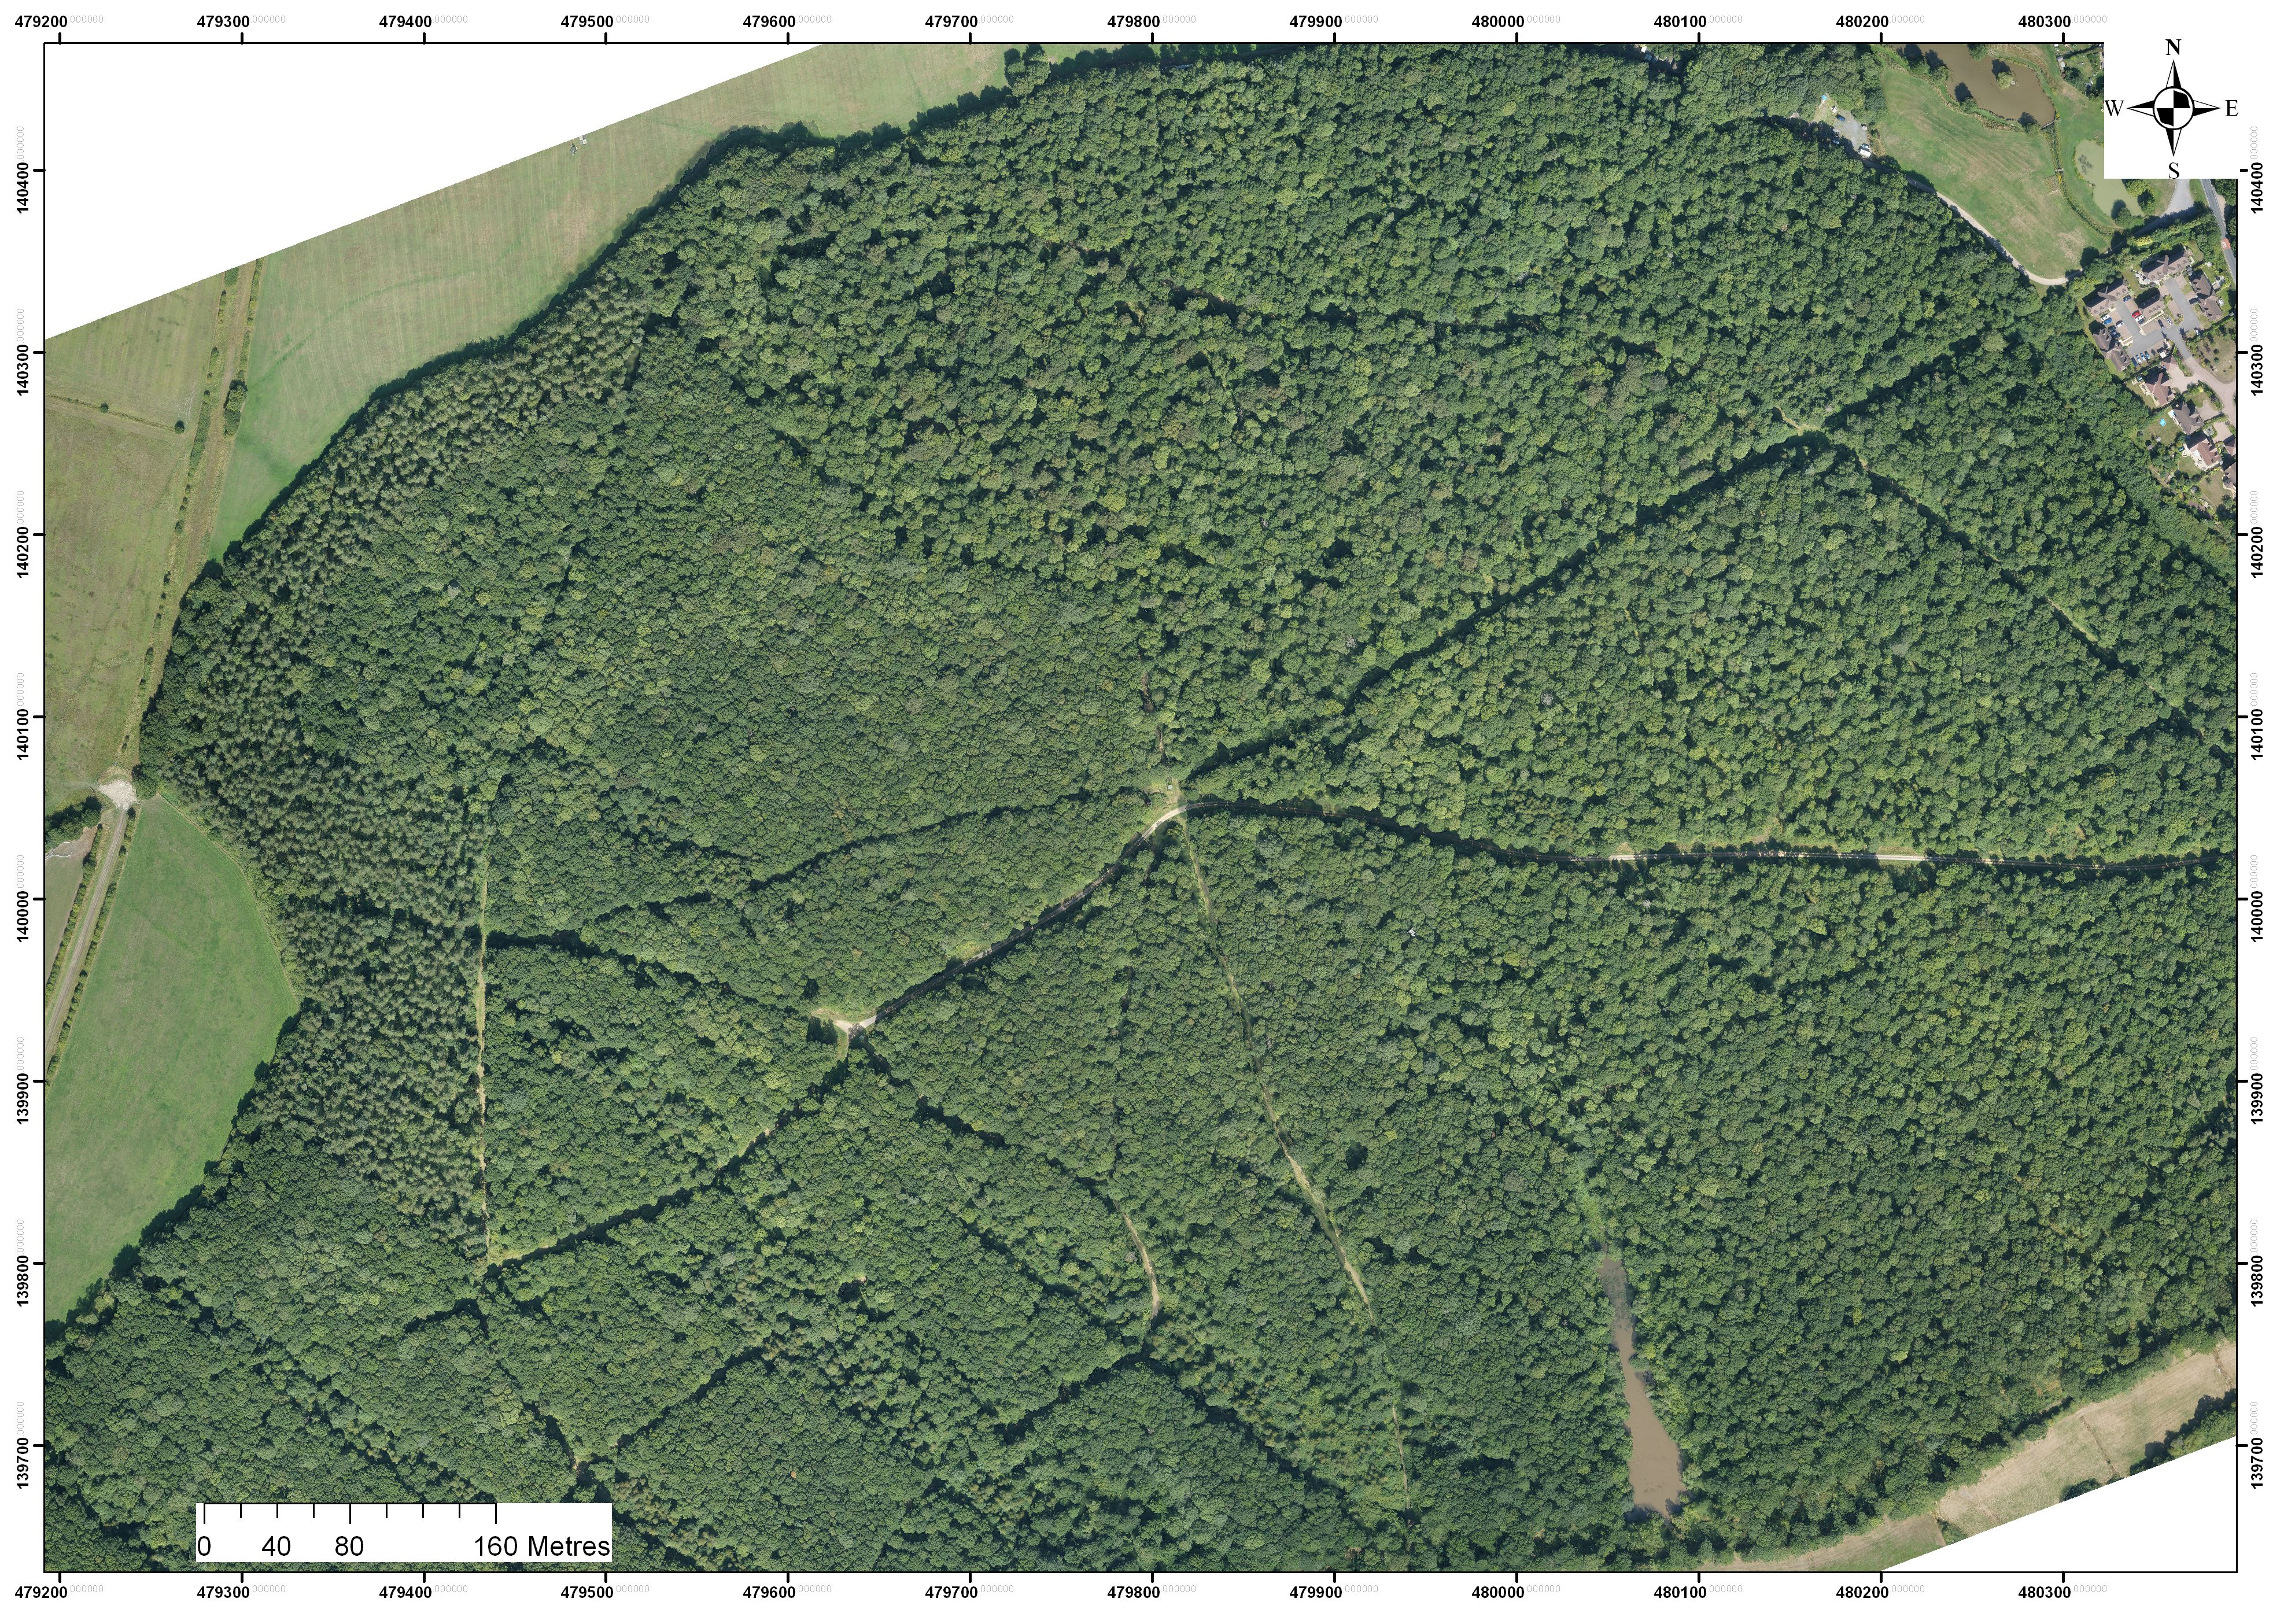
\includegraphics[width=0.8\textwidth]{chapter/chapter4/AP1_2013.jpg}
    \caption{The Straits Inclosure research site in 2013.} \label{fig:ah_aerial_photo}
\end{figure}

\section{Establishment of sampling points}

For this fieldwork transects were designed to join up existing mensuration plots where measurements of woody biomass are made by Forest Research. This allowed for comparison with historic observations. In total 435 sampling points were marked at 10m intervals, these are shown in Figure~\ref{fig:transects}. Python was used to calculated the exact latitude and longitude of each sampling point for the 3 transects, these locations were then entered into a GPS unit. When establishing the transects fluorescent spray paint was used to mark trees closest to each sampling point as shown on the GPS (see Figure~\ref{fig:pink_tree}). As parts of the forest site were extremely dense with vegetation a pair of loppers were used to clear a path in some areas to allow for the construction of relatively straight transects. Having all transect points numbered and corresponding to a latitude and longitude value allowed for comparison between methods and the splitting of observations between different distinct sections of the forest site. 


\begin{figure}[ht]
    \centering
    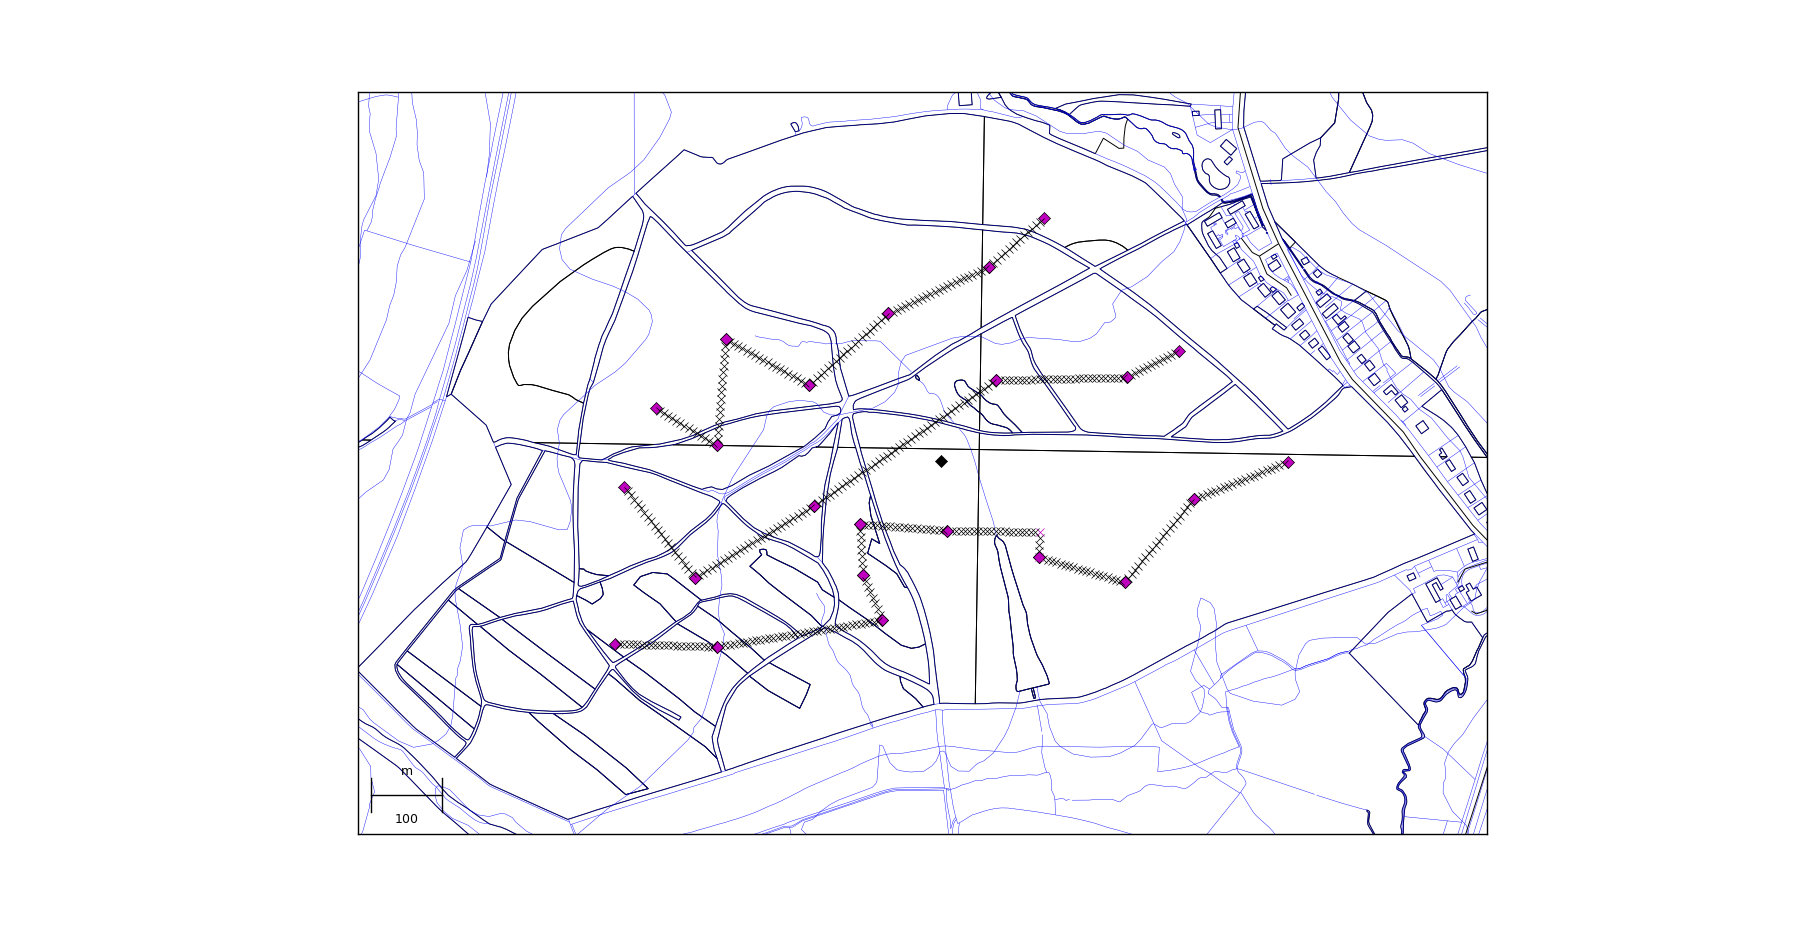
\includegraphics[width=\textwidth]{chapter/chapter4/straitsmap_threet_10m.png}
    \caption{Sampling transects. Black crosses: sampling points at 10m intervals, pink diamonds: Forest Research mensuration plots, black diamond: Forest Research flux tower.} \label{fig:transects}
\end{figure}

\begin{figure}[ht]
    \centering
    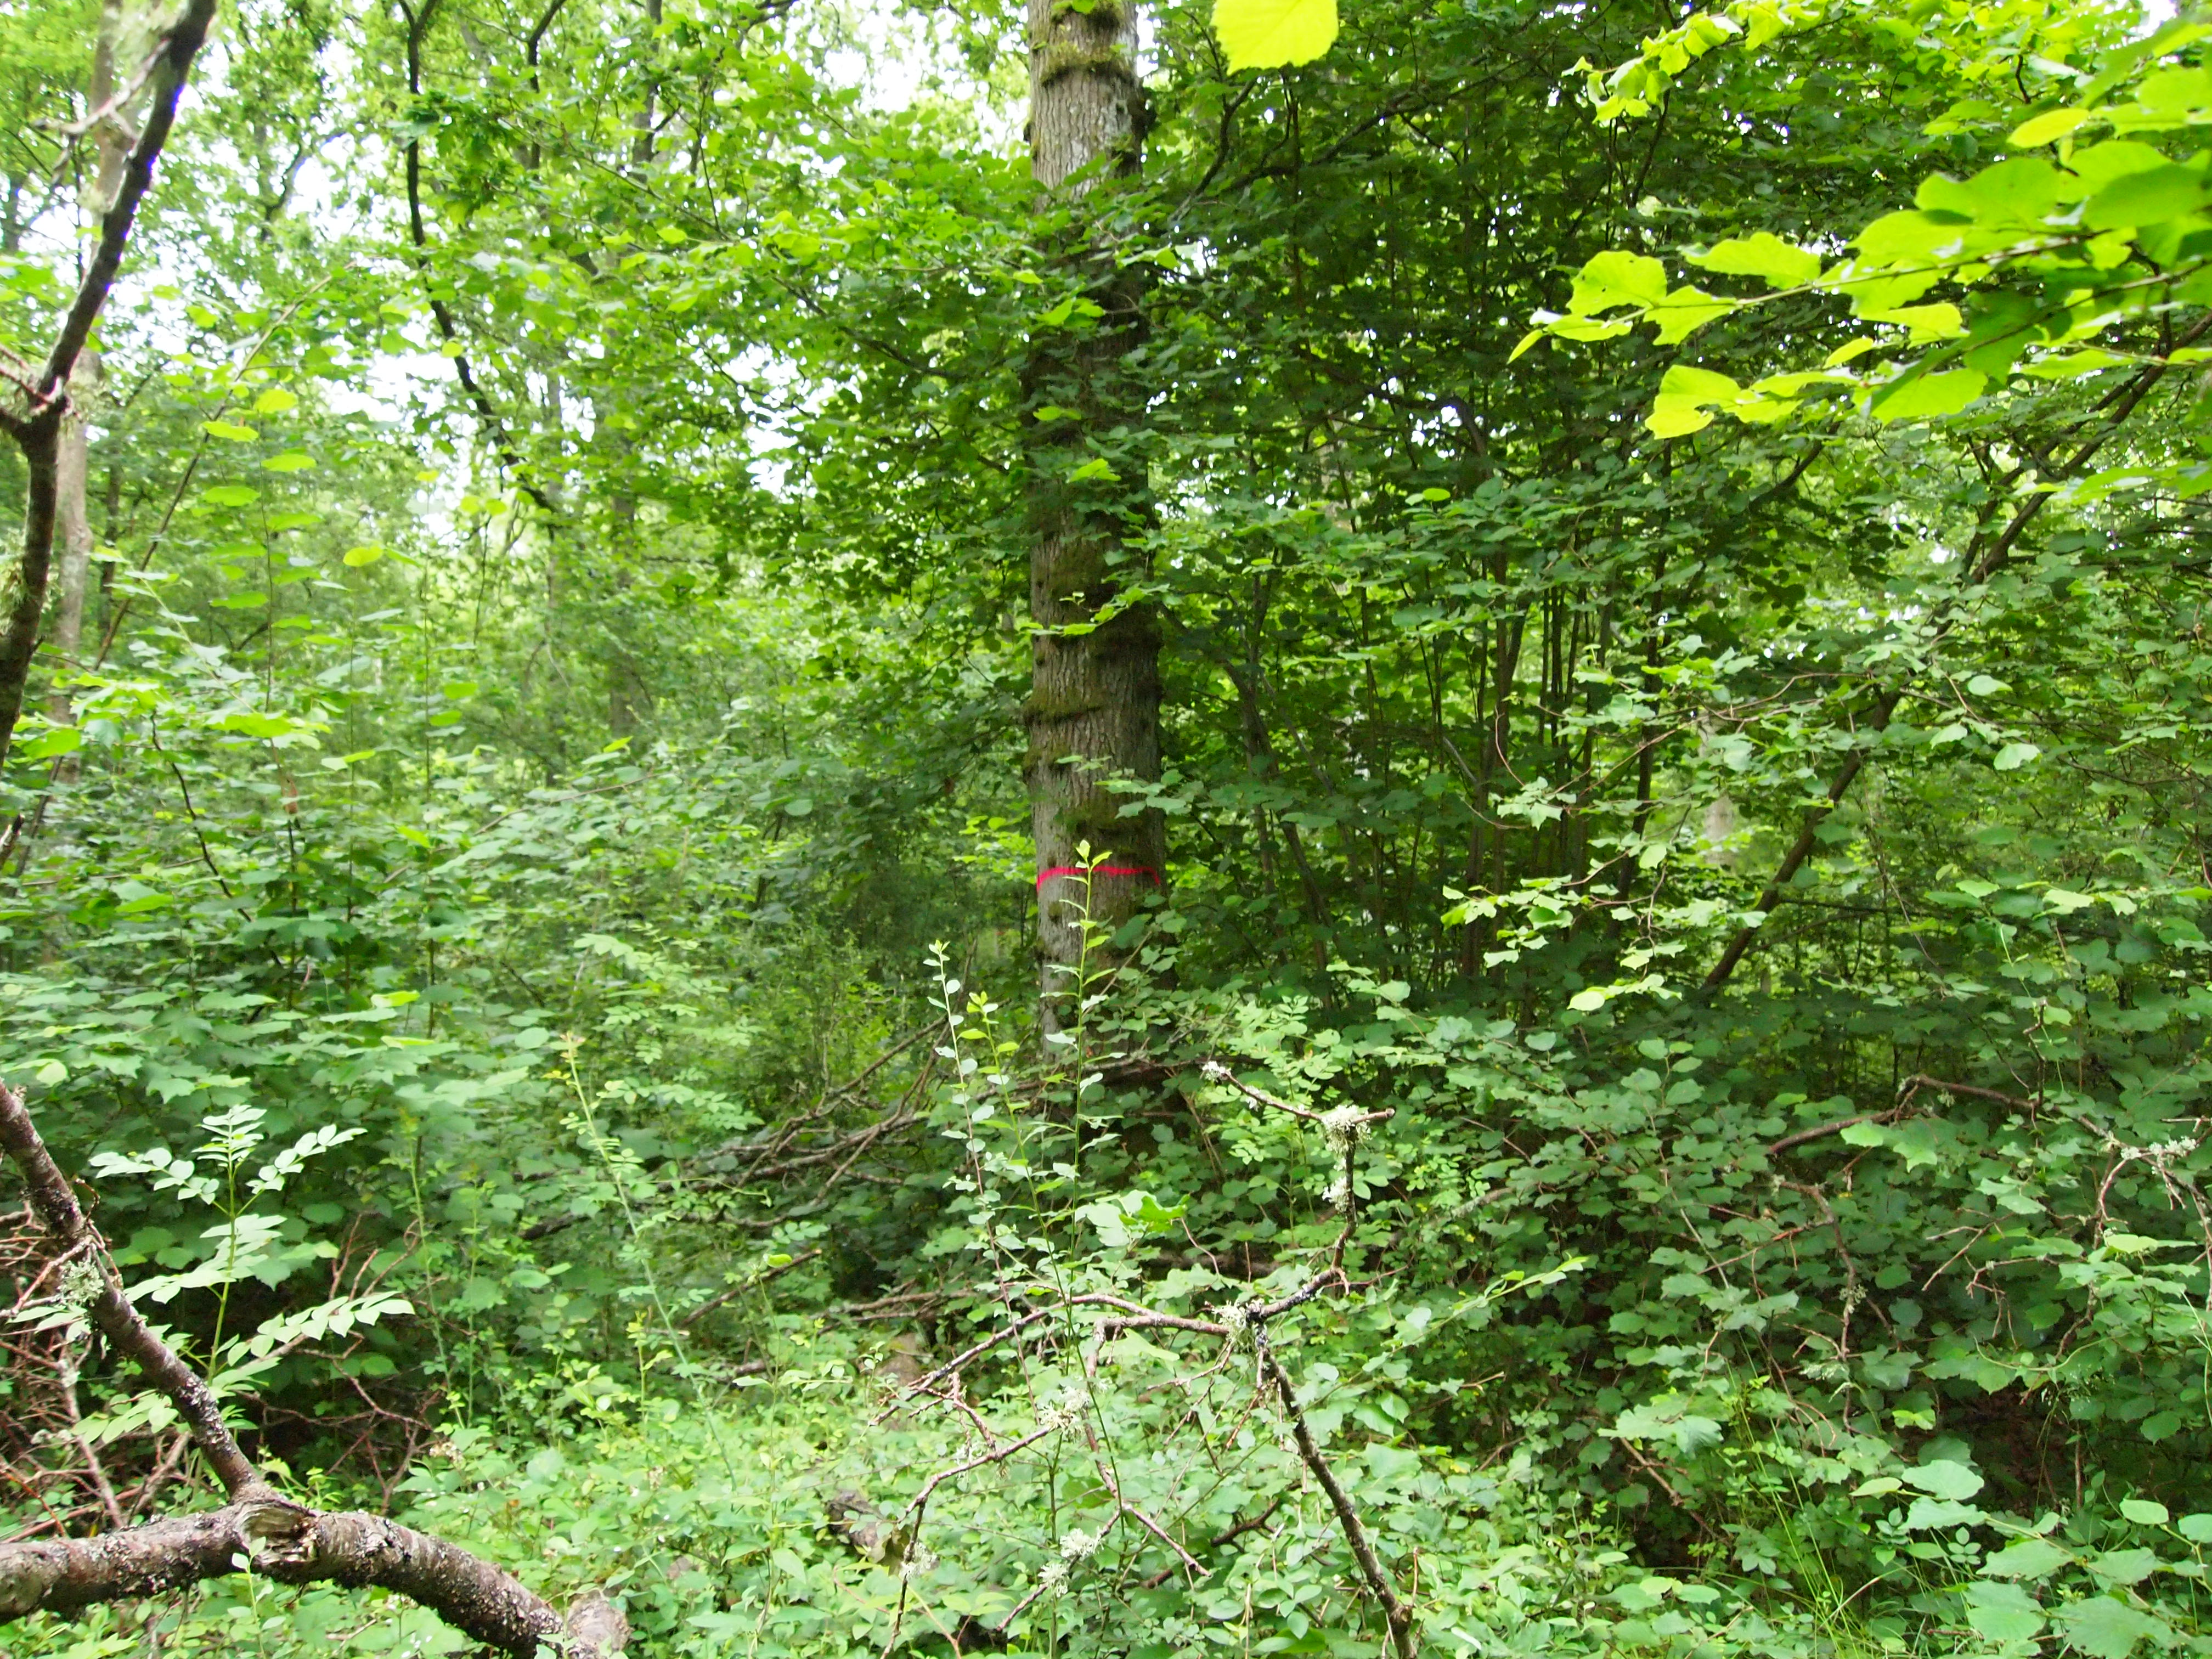
\includegraphics[width=0.8\textwidth]{chapter/chapter4/291E.jpg}
    \caption{Sampling point 291, showing fluorescent spray paint used to mark sampling points.} \label{fig:pink_tree}
\end{figure}

\section{Leaf area index observations}

Leaf Area Index (LAI) is an important variable in relation to the amount of CO\(_2\) an ecosystem can remove from the atmosphere through photosynthesis. LAI is defined as the area of leaves per unit area of ground. Three different methods were used to find estimates for peak LAI (July - September) for the year 2015 along the three transects at different sampling intervals.

\subsection{Ceptometer}

A Decagon LP-80 ceptometer and an additional Photosynthetically Active Radiation (PAR) sensor were used to measure LAI. Here we measure below canopy PAR using the ceptometer while logging above canopy PAR using a data logger and PAR sensor positioned outside the canopy. We can then calculate LAI using the above and below canopy readings and a set of equations relying on some assumptions \citep{fassnacht1994comparison}. The ceptometer represents the quickest method for estimating LAI, we therefore took readings with the ceptometer at every sampling point over two walks of the transects, giving us 870 observations in total.

In order to be sure that the PAR readings from the ceptometer and external PAR sensor were consistent we had to calibrate the PAR sensor against the ceptometer. This was done by leaving both the PAR sensor and ceptometer out logging next to each other every 10 seconds for a day in the Alice Holt Research Station met square. We can then calibrate he output of the PAR sensor with that of the ceptometer as shown in Figure~\ref{fig:par_calib}. 

\begin{figure}[ht]
    \centering
    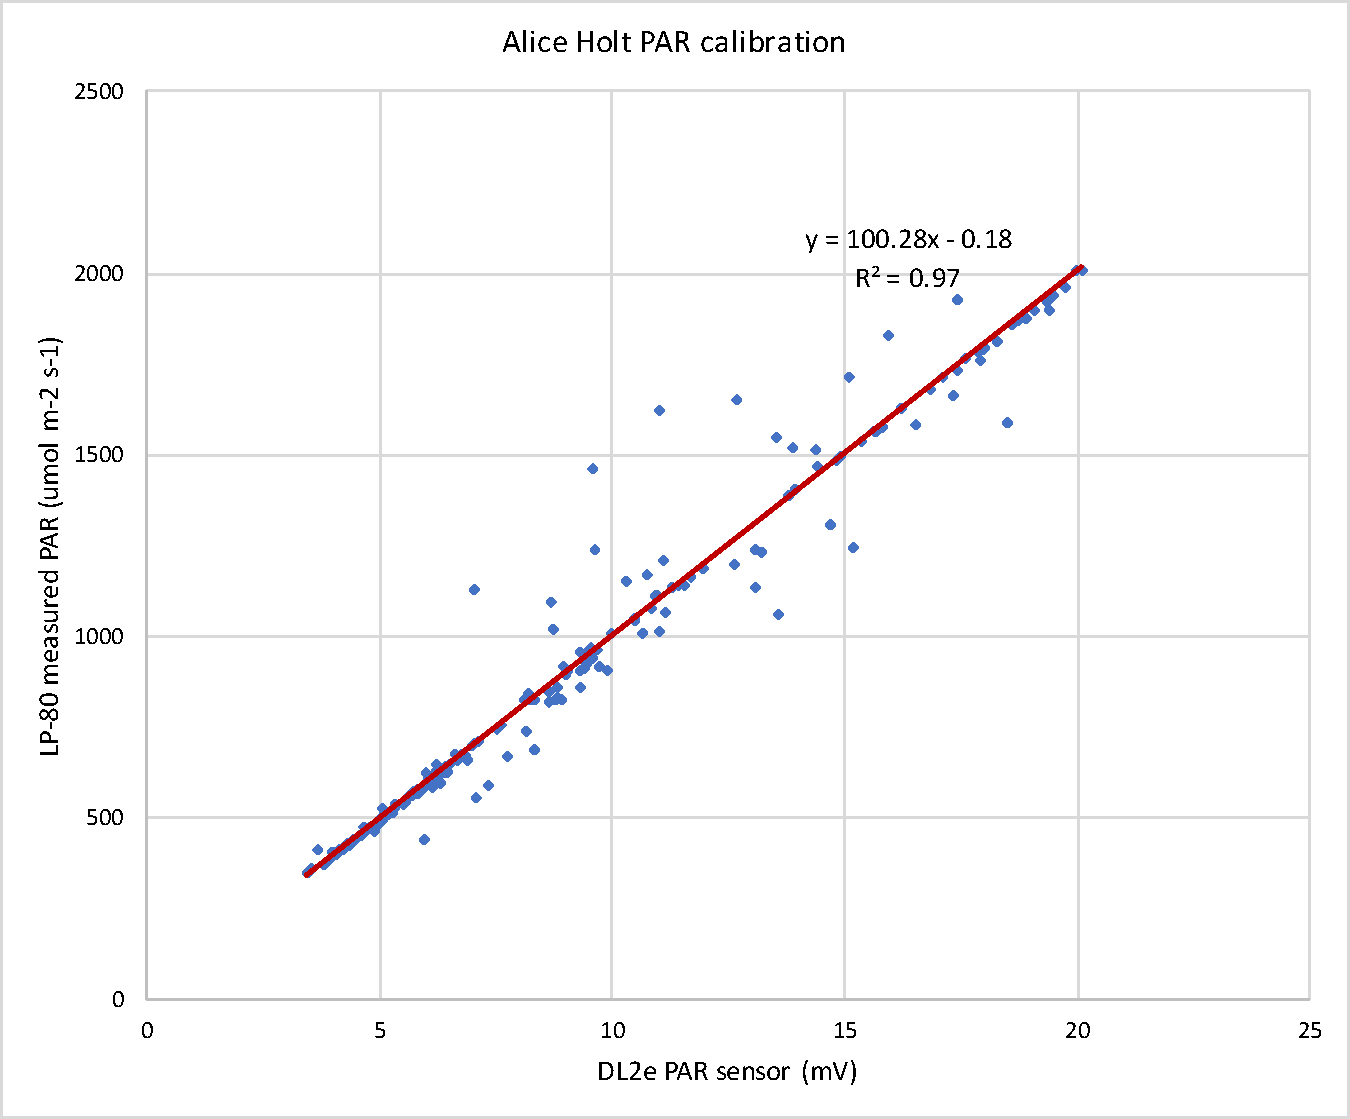
\includegraphics[width=0.8\textwidth]{chapter/chapter4/AH_PAR.pdf}
    \caption{Calibration of above canopy Photosynthetically Active Radiation (PAR) sensor (measuring in mV) with LP-80 ceptometer measured PAR (\(\mu \text{mol}~\text{m}^{-2}~\text{s}^{-1} \)).} \label{fig:par_calib}
\end{figure}

Once the PAR sensor was calibrate measurements could be made along the transects. The PAR sensor positioned outside of the canopy was logged every 5 seconds using a Delta-T DL2e data logger, at the start of every set of measurements the clock on the data logger and ceptometer were synchronised to ensure comparison of measurements made at the same time. After sampling the transects we had a set of above canopy and below canopy PAR readings corresponding to each sampling point for both walks of the transects. We use the same calculation for LAI as given in the Decagon LP-80 manual. This is using a simple model of radiation transmission and scattering tested against the more complex model of \citet{norman1975photosynthesis}. The equation used to calculate LAI from the above and below canopy PAR readings is,
\begin{equation}
LAI = \frac{((1-\frac{1}{2K})f_b - 1)\text{ln}\tau}{A(1-0.47f_b)},
\end{equation} 
where \(K\) is the extinction coefficient, \(f_b\) is the beam fraction, \(\tau = \frac{\text{below canopy PAR}}{\text{above canopy PAR}}\) and \(A = 0.283 + 0.785a - 0.159 a^2\) (where a is the leaf absorptivity, assumed to be 0.9 by Decagon). We assume a spherical leaf angle distribution parameter, \(\chi = 1\), this means the extinction coefficient simplifies to \(K=\frac{1}{2\text{cos}\theta}\), where \(\theta\) is the solar zenith angle. We took the mean of the two LAI observations at each point to give as an estimate to the peak LAI for the year 2015. We can see the LAI estimate for the Straits Inclosure in Figure~\ref{fig:cept_lai}. 

\begin{figure}[ht]
    \centering
    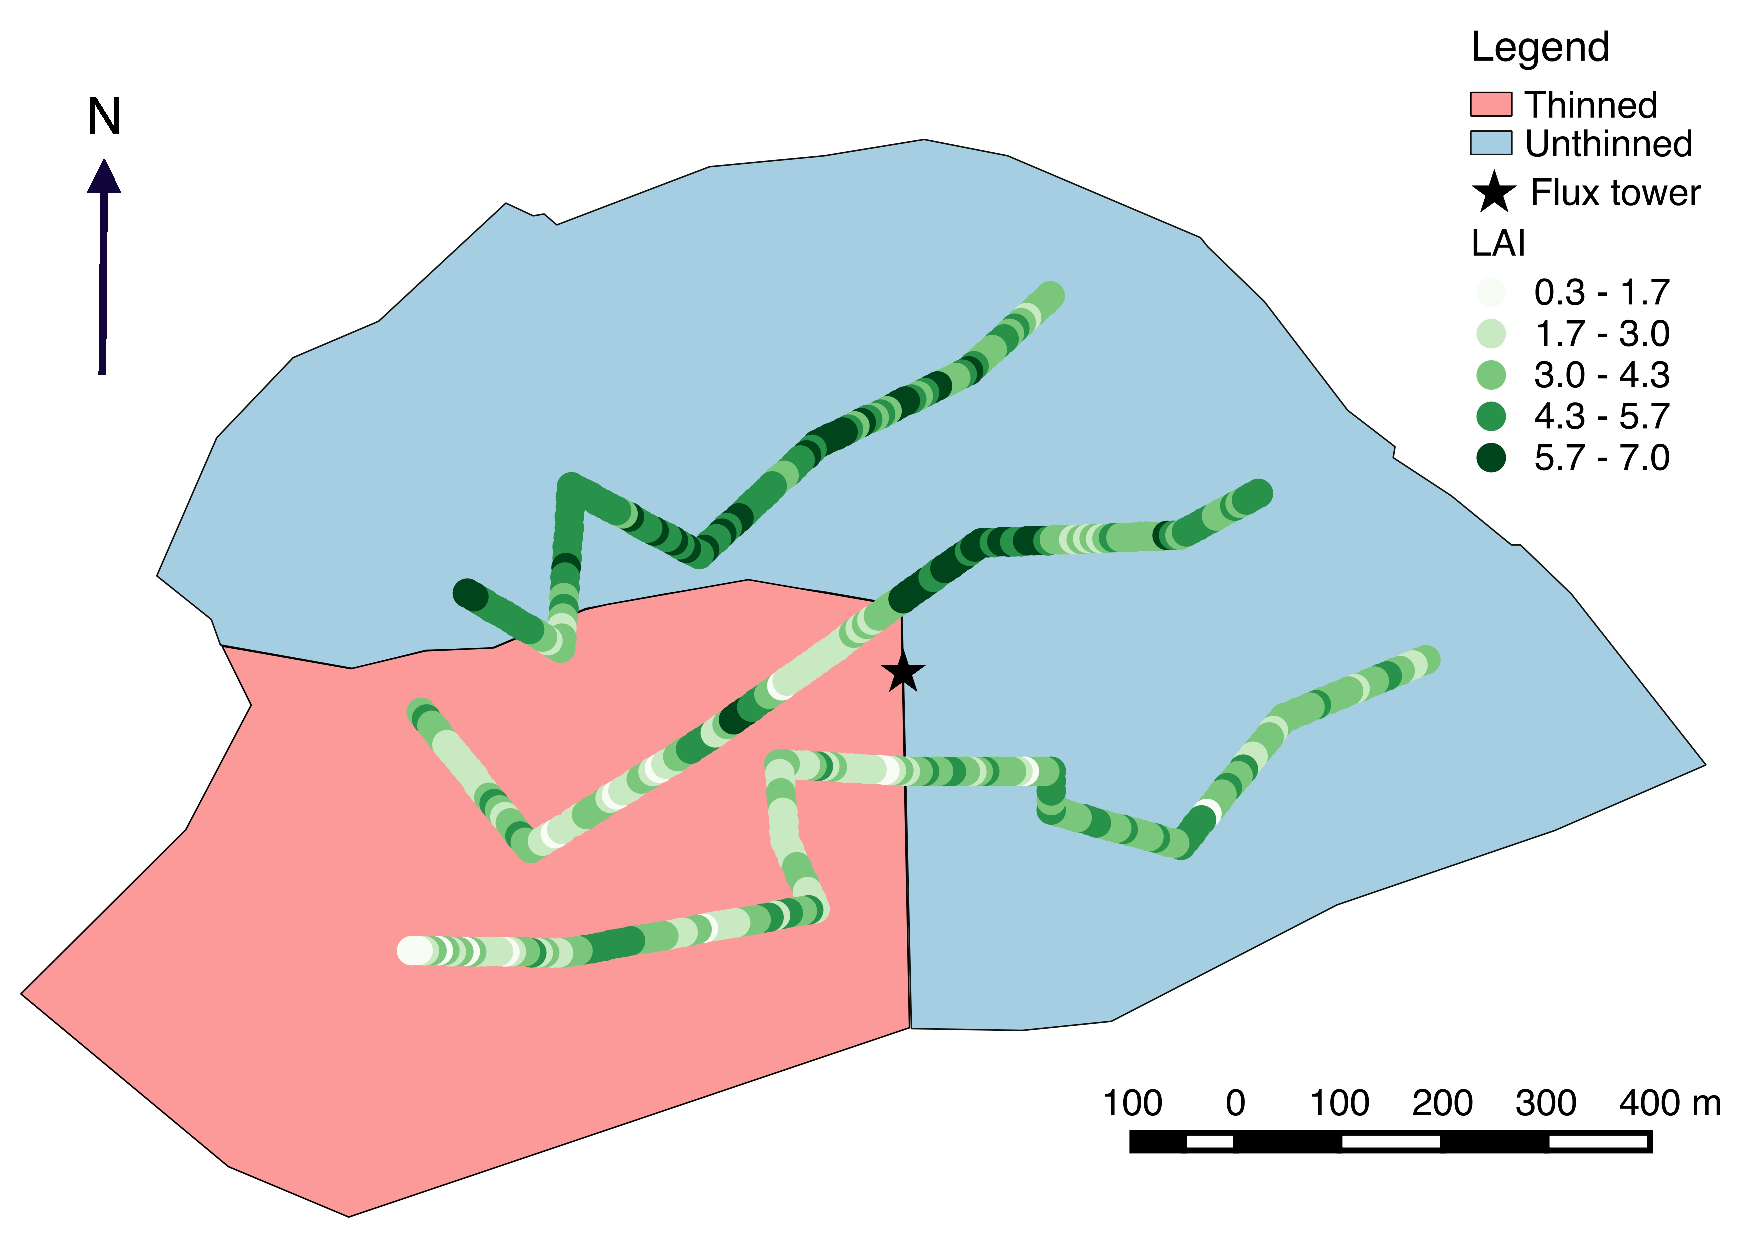
\includegraphics[width=0.8\textwidth]{chapter/chapter4/lai_cept.pdf}
    \caption{Ceptometer derived LAI for Alice Holt.} \label{fig:cept_lai}
\end{figure}

\subsection{Hemispherical photographs} \label{sec:hemi_photos}

The next method used to measure LAI was hemispherical photography. Hemispherical photographs show a complete view of the sky in all directions, from these images we use the HemiView software \citep{rich1999hemiview} which calculates the proportion of visible sky as a function of sky direction (gap fraction) which it then uses to calculate LAI \citep{Jonckheere2004}. Hemispherical photographs were taken every 50m along the transects, giving a total of 89 images. It is important to that hemispherical photographs are taken in overcast conditions so that the sun does not obscure areas of leaf area. It is important to note that we did not remove tree trunks and branches from our calculation of LAI with HemiView so that we are actually calculating plant area index. The impacts of this assumption are discussed in section~\ref{sec:lai_comp}. In Figure~\ref{fig:hemiphotos} we show an example of two hemispherical photographs taken in different areas of the Straits Inclosure.

\begin{figure}[ht]
\centering
\begin{subfigure}{.5\textwidth}
  \centering
  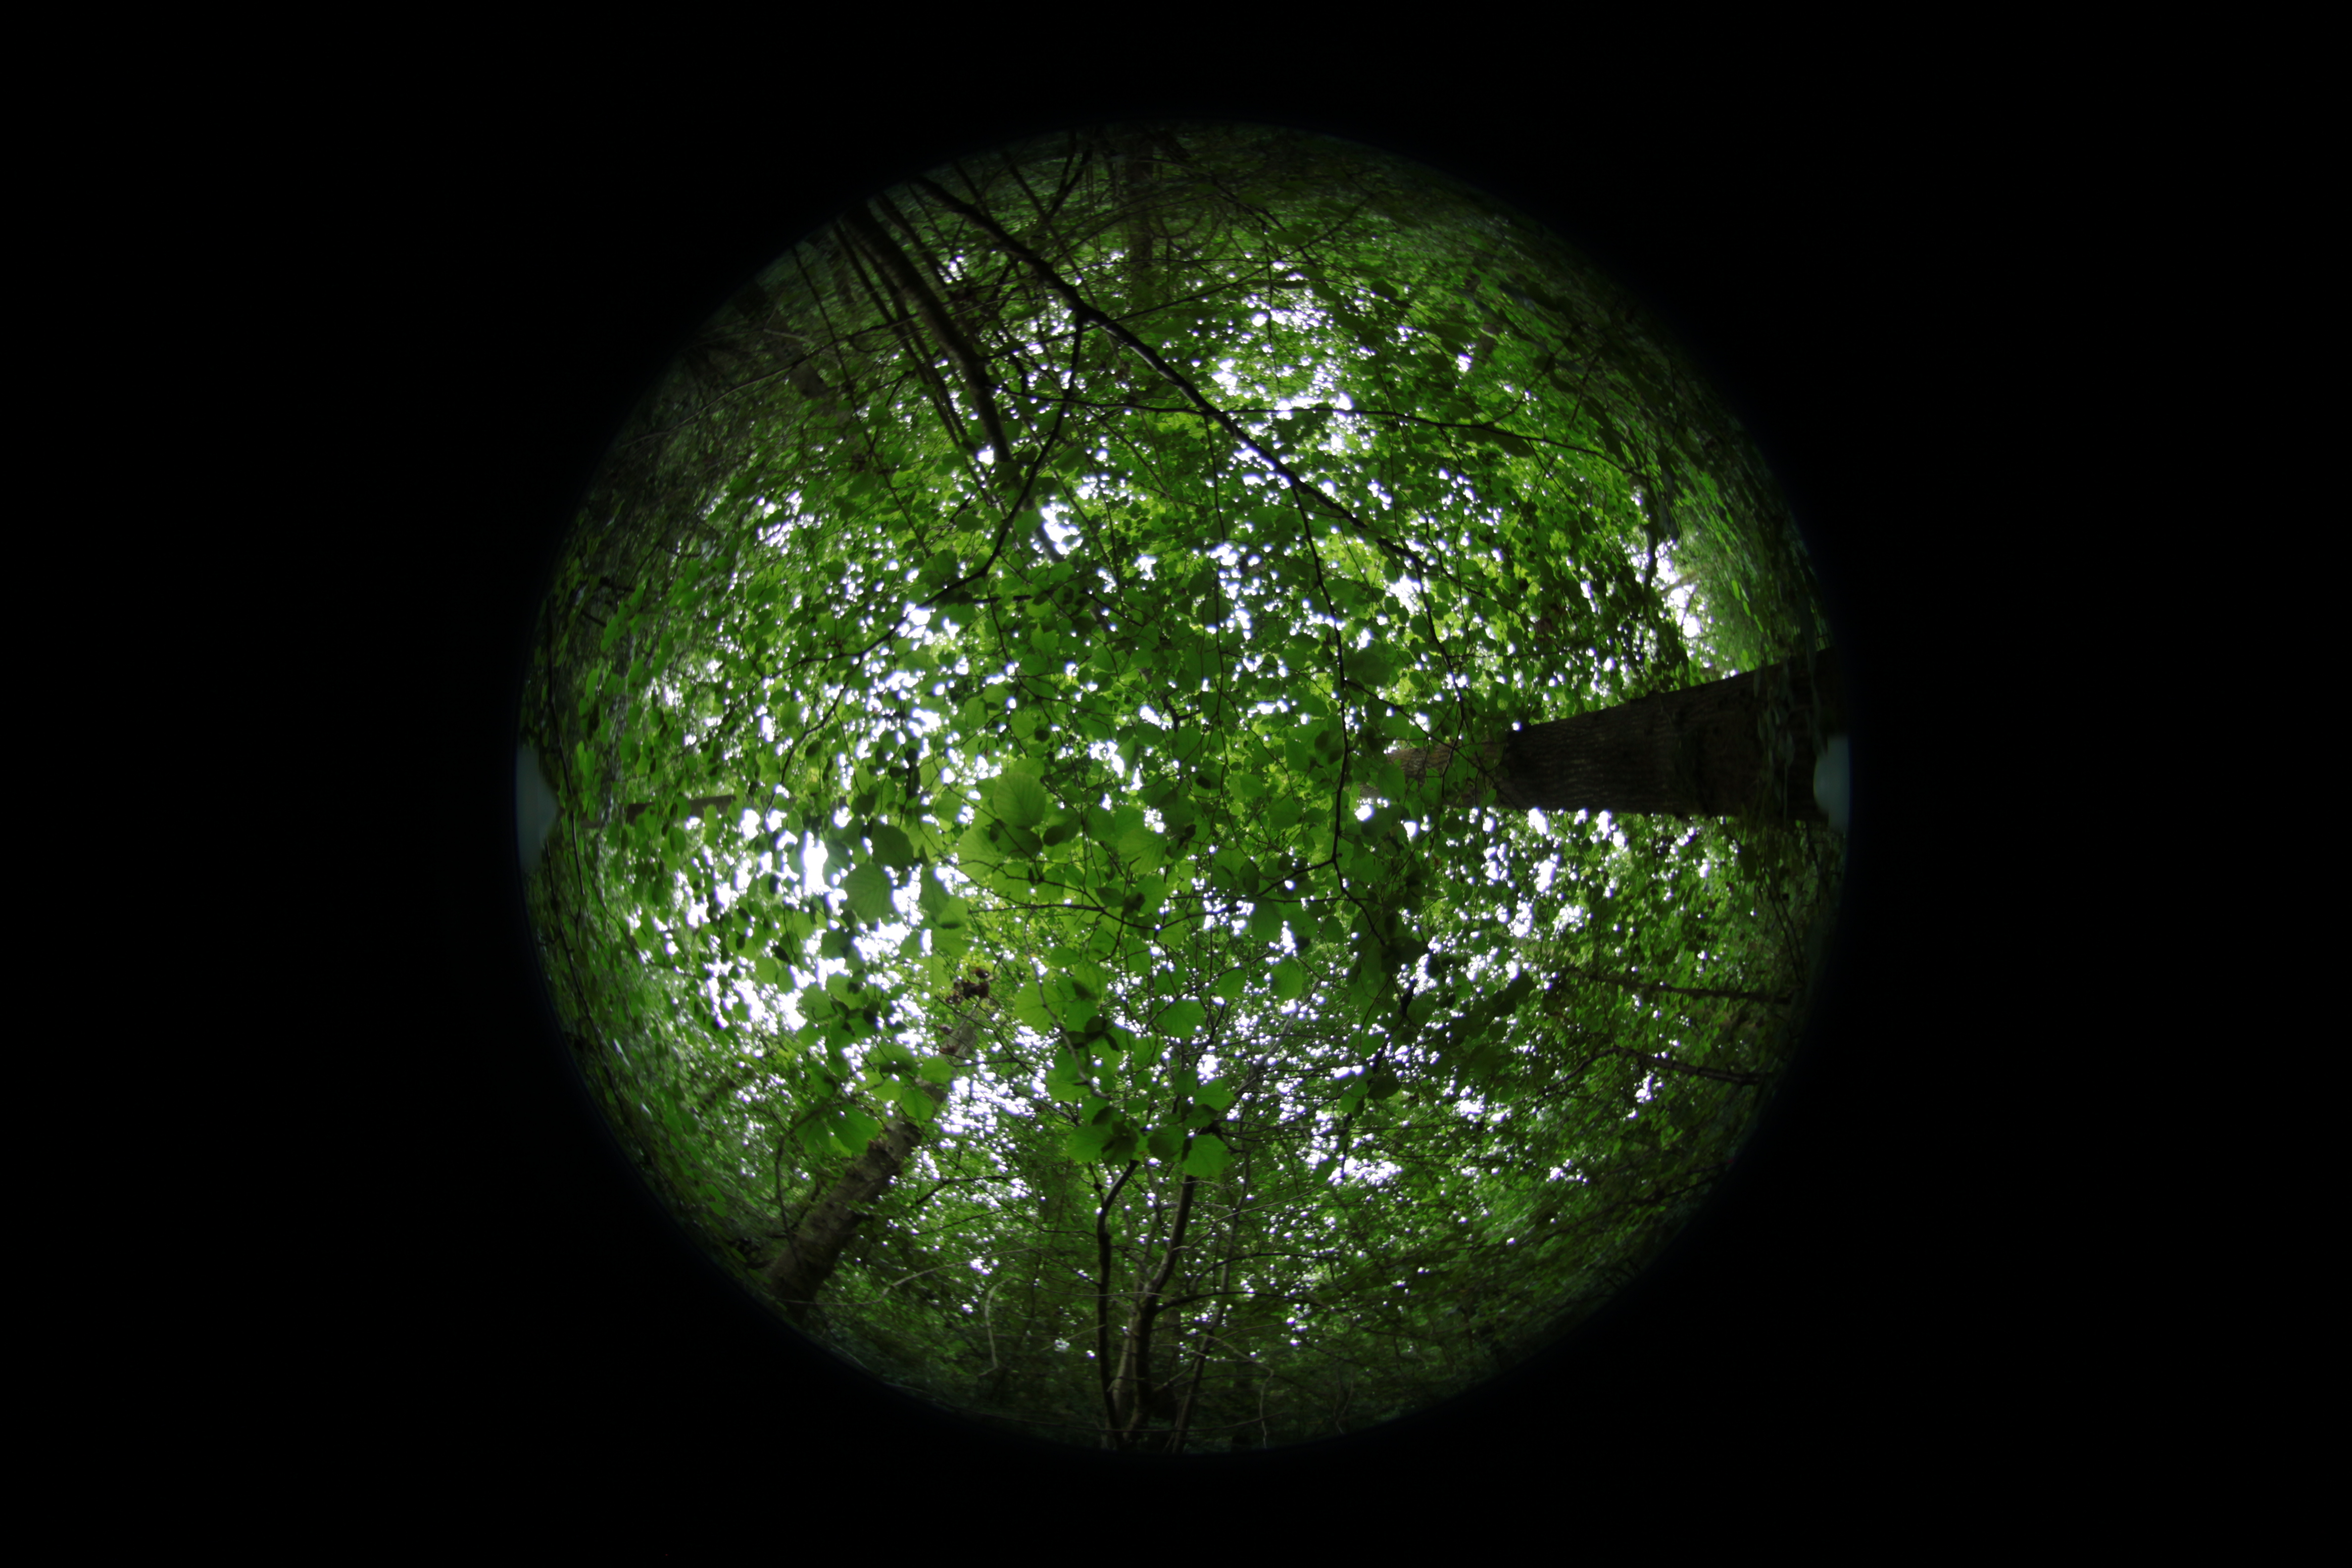
\includegraphics[width=.9\linewidth]{chapter/chapter4/043exp2.jpg}
  \caption{Unthinned forest}
  \label{fig:sub1}
\end{subfigure}%
\begin{subfigure}{.5\textwidth}
  \centering
  \includegraphics[width=.9\linewidth]{chapter/chapter4/252exp1.jpg}
  \caption{Thinned forest}
  \label{fig:sub2}
\end{subfigure}
\caption{Hemispherical photographs from the Alice Holt flux site showing the difference between the thinned and unthinned sides of the forest.}
\label{fig:hemiphotos}
\end{figure}

\subsection{Litter traps}

Finally litter traps were used to find estimates to LAI and leaf mass per area. Here we placed litter traps under the canopy to catch leaf litter as it falls into a bag attached to the bottom of the trap. The bags were changed every week during the litter fall period and the litter sorted into species. Every week the litter was dried in an oven at $70^{\text{o}}\text{C}$ and weighed. This gave us the dry-weight of the leaf litter for the 2015 season. Towards the end of the season we scanned a subsample for each species of 100 leaves to find an area, we then dried and weighed each subsample, a relationship between dry-weight and leaf area was then be built (leaf mass per area) and used to infer the total LAI for each trap once the whole seasons litter has been collected. This method of LAI calculation is the most time consuming.  

A total of six litter traps were established at points along the transects (positions shown in Figure~\ref{fig:lit_traps}) allowing for comparison with the other methods. The 6 litter traps are not enough to describe the LAI for the research site \citep{kimmins1973some}. We use these litter traps as a point of comparison and validation for the ceptometer and hemispherical photograph estimates of LAI made at the same locations and also for estimates to leaf mass per area. From our litter trap observations we find a leaf mass per area of 29~g~C~m\(^{-2}\) free soluble carbohydrates for both sides of the forest.

\begin{figure}[ht]
    \centering
    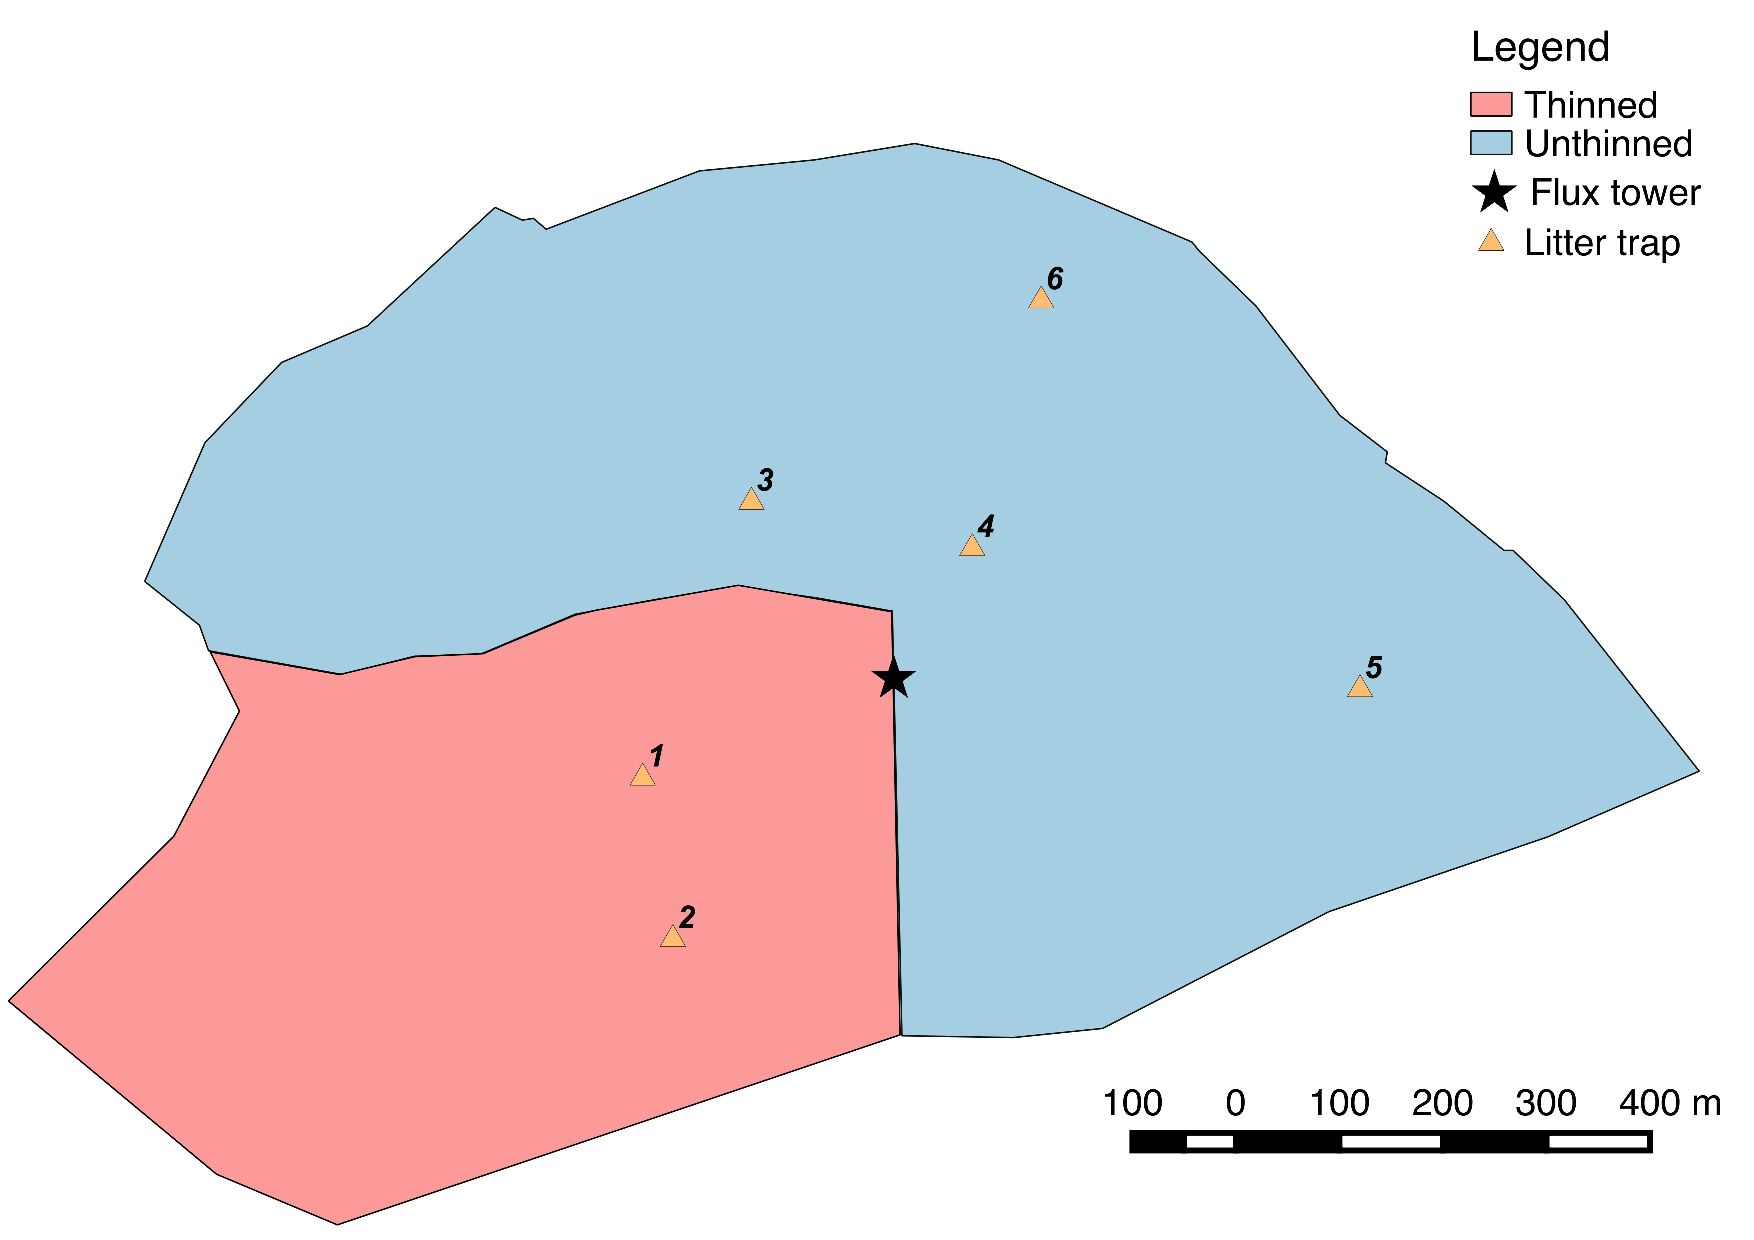
\includegraphics[width=0.8\textwidth]{chapter/chapter4/litter_trap.pdf}
    \caption{Litter trap locations for Alice Holt.} \label{fig:lit_traps}
\end{figure}


\subsection{Comparison of methods} \label{sec:lai_comp}

In Figure~\ref{fig:lai_comp07} and \ref{fig:lai_comp14} we show a comparison of the different methods of estimating LAI for the unthinned and thinned forest respectively. We can see that in all cases LAI derived from the litter traps is always greater than LAI estimated from optical methods, this is expected from previous comparisons \citep{breda2003ground}.
 
Although the ceptometer is the fastest method for measuring LAI it is also the most variable, being extremely sensitive to the solar zenith angle and clear sky conditions. If the sun is low in the sky the radiation will pass through much more photosynthetically active material than if the sun is directly above head, causing spikes in the LAI value. We can see that the LAI estimates from the hemispherical photographs are much less variable than the ceptometer. As discussed in section~\ref{sec:hemi_photos} the hemispherical estimate is actually of plant area index, as we have not removed trunks and branches from the gap fraction calculation. However, this does not appear to have a great impact on results as hemispherical photograph derived LAI is still the lowest estimate of all three. 

\begin{figure}[ht]
    \centering
    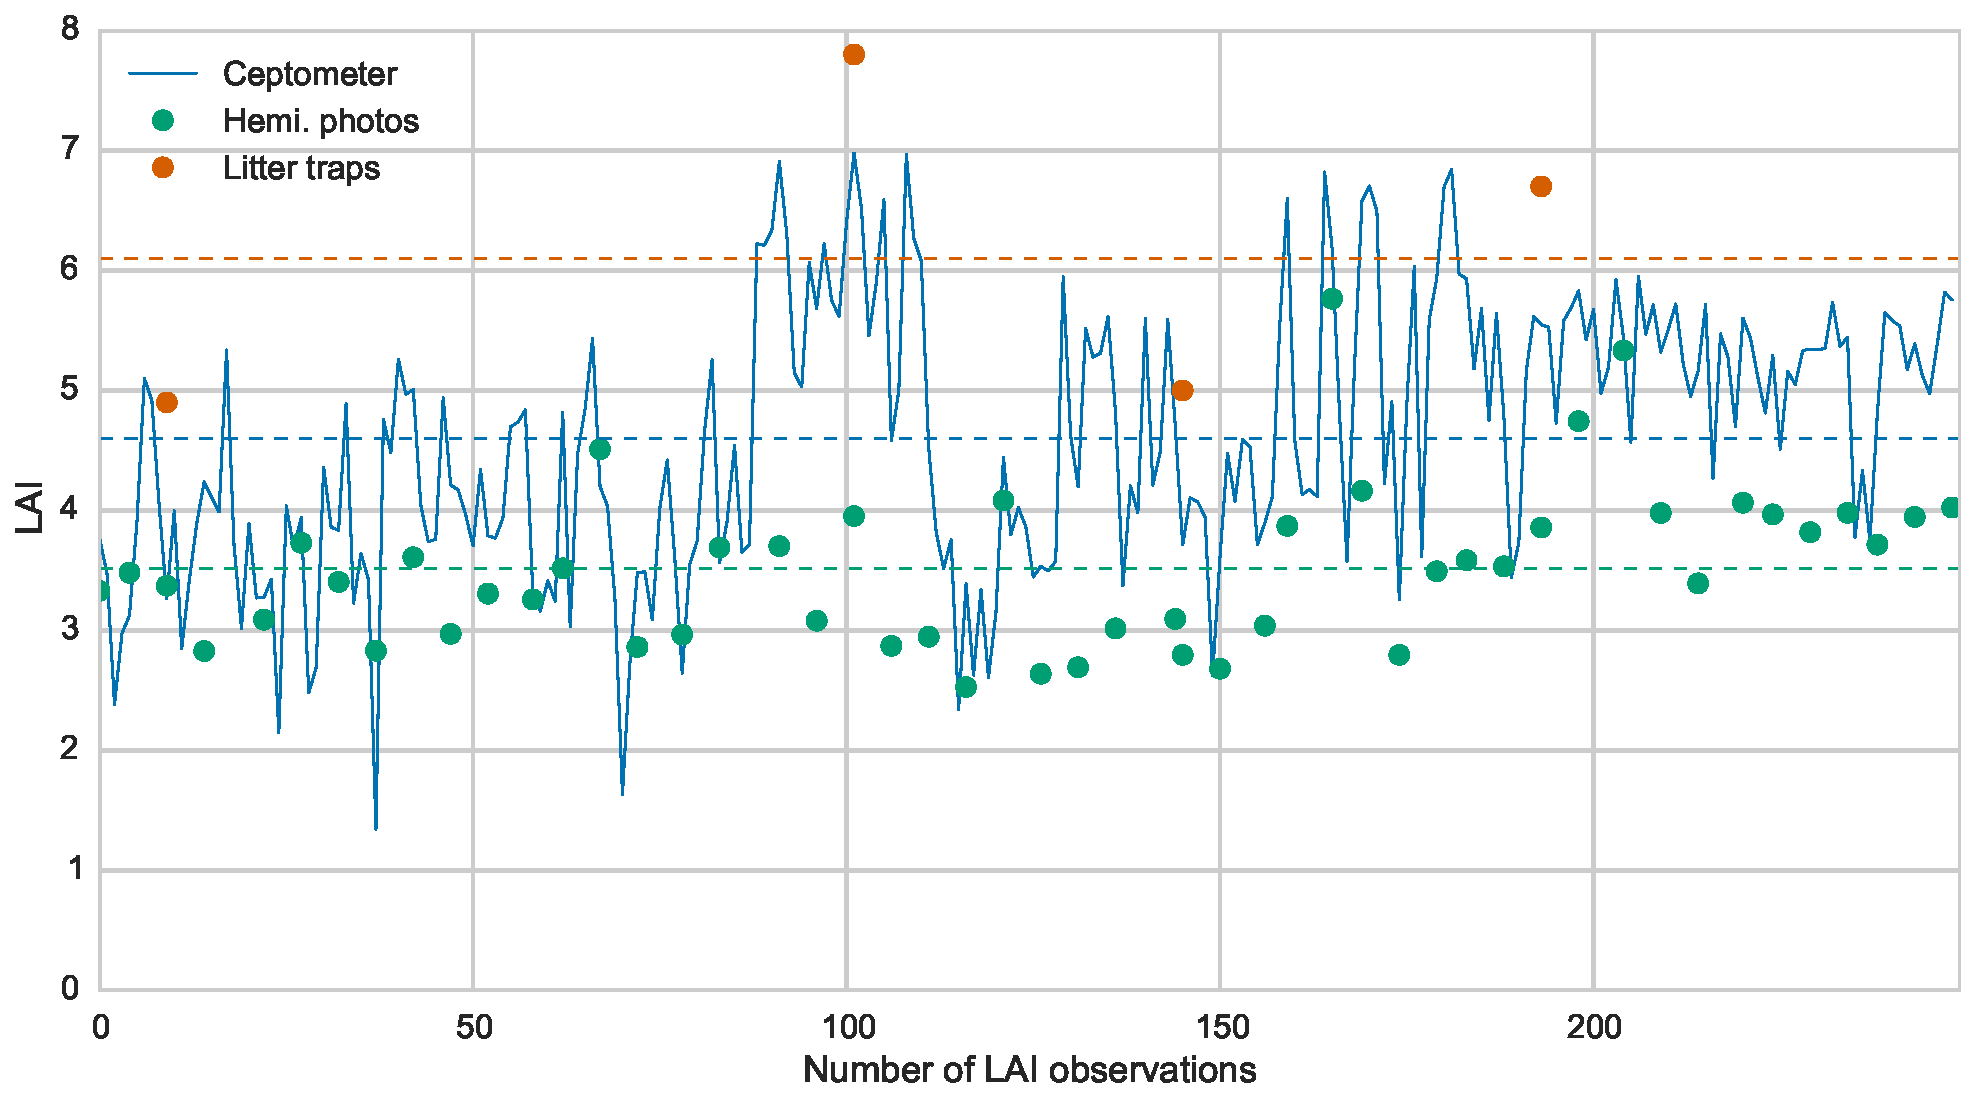
\includegraphics[width=0.8\textwidth]{chapter/chapter4/thinned07.pdf}
    \caption{LAI comparison for unthinned forest. Dots and solid line represent observations made at different points along transects, dotted lines represent the mean of the observations.} \label{fig:lai_comp07}
\end{figure}

\begin{figure}[ht]
    \centering
    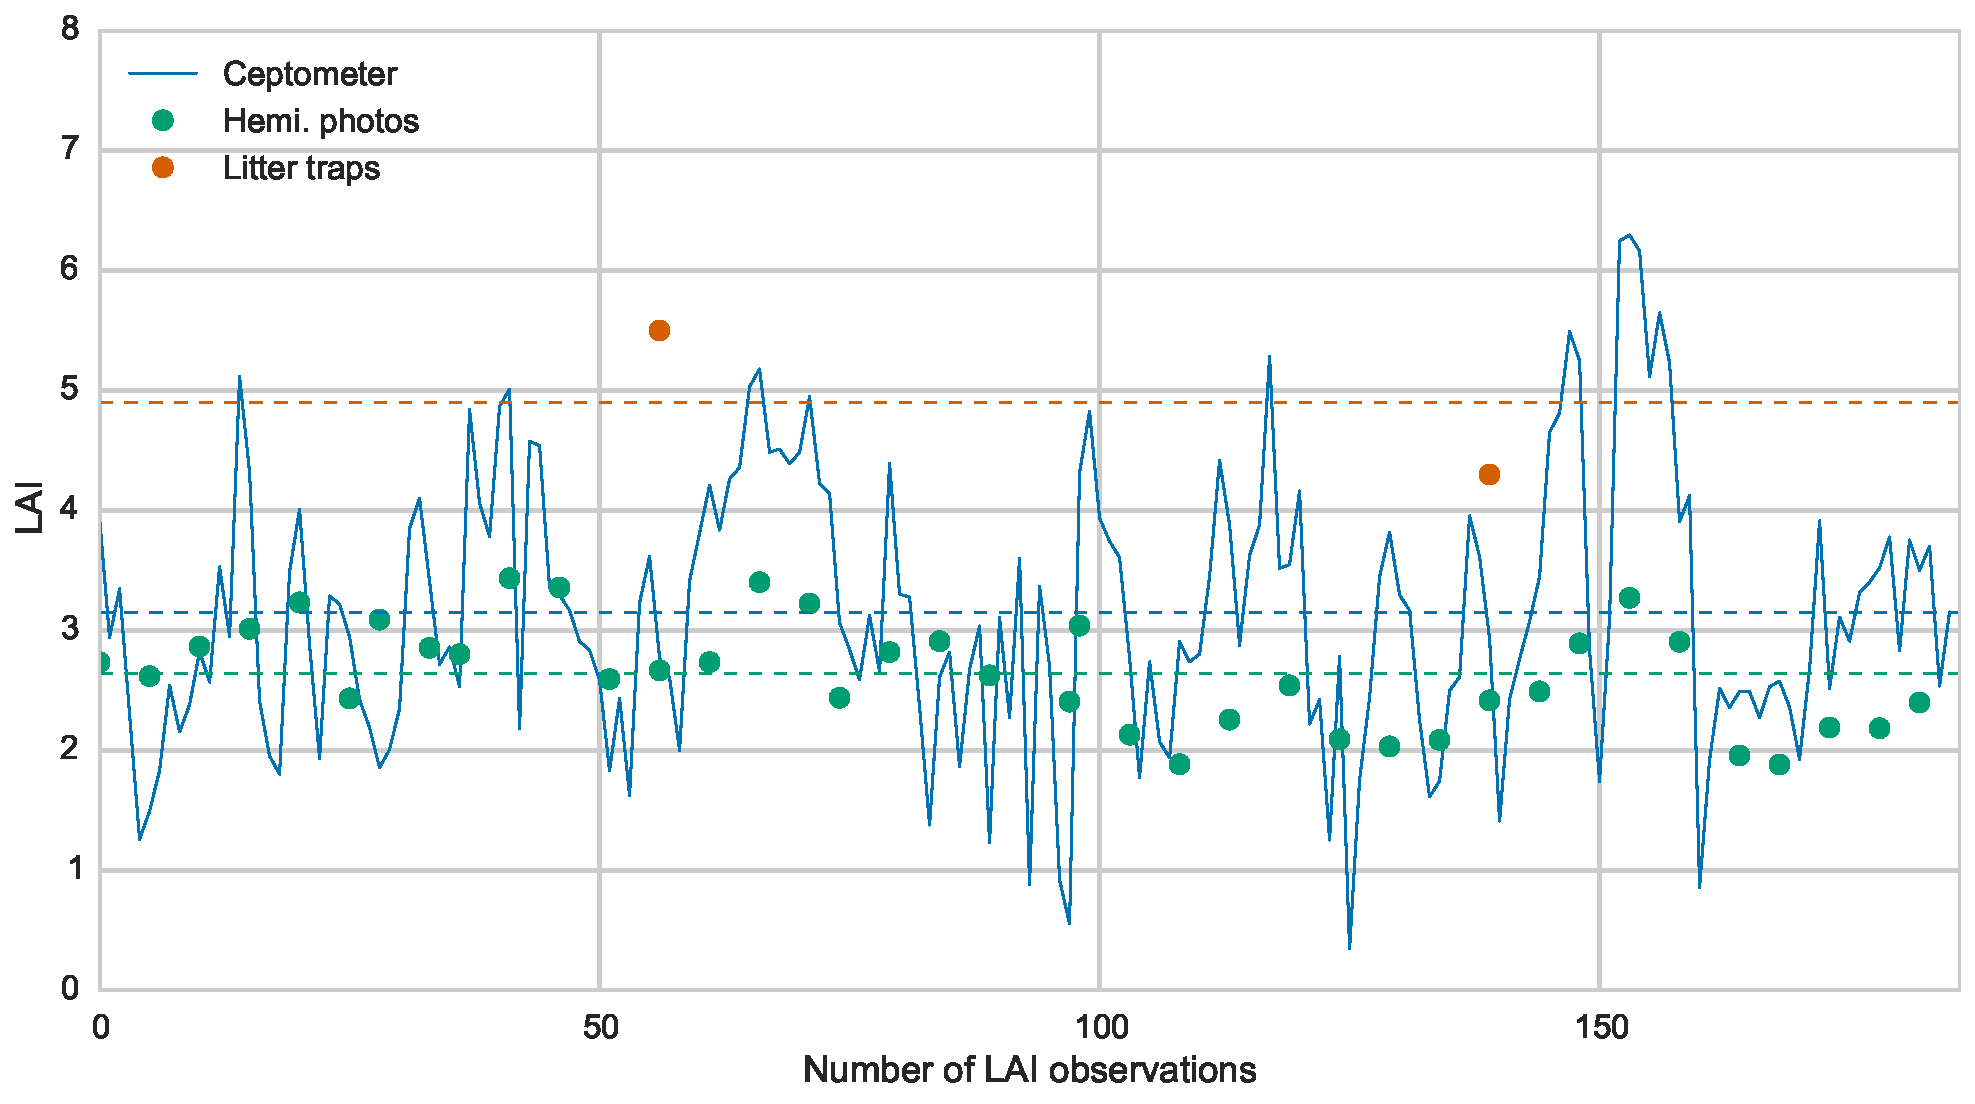
\includegraphics[width=0.8\textwidth]{chapter/chapter4/thinned14.pdf}
    \caption{LAI comparison for thinned forest. Dots and solid line represent observations made at different points along transects, dotted lines represent the mean of the observations.} \label{fig:lai_comp14}
\end{figure}

\section{Point-centred quater observations}

We used the method of Point-Centred Quarters (PCQ) \citep{dahdouh2006empirical} to determine an estimate of the woody biomass for both unthinned and thinned forest in the Straits Inclosure. The PCQ method is conducted at each sampling point as follows:
\begin{itemize}
\item Using a compass, map 4 regions from the central sampling point
\item Measure the distance from the central sampling point to the nearest tree in each quarter
\item Measure the Diameter at Breast Height (DBH) for each tree (shown in Figure~\ref{fig:dbh_me}) and record the species 
\end{itemize}
There were 114 points samples along the three transects, from these measurements we derived estimates to tree density and mean DBH for both thinned and unthinned sides of the forest. We then used allometric relationships between DBH and total above ground biomass and coarse root biomass, found in work carried out by Forest Research and in \citet{mckay2003woodfuel}. These relationships were as follows,
\begin{equation}
\text{above ground dry-mass} = 0.0678\times \overline{\text{DBH}}^{2.619}
\end{equation}
and
\begin{equation}
\text{below ground coarse root dry-mass} = 0.149\times \overline{\text{DBH}}^{2.12}.
\end{equation}

This gave us an estimate to the dry-mass in kilograms for the average tree in our sampling area. Assuming that half of all dry-mass is carbon we can find an estimate of total woody and coarse root carbon in g~C~m\(^{-2}\) using the equation,
\begin{multline}
\text{total woody and coarse root carbon} =  \\1000\times0.5\times(\text{above ground dry-mass} + \text{below ground coarse root dry-mass})\times \text{tree density}.
\end{multline}

Forest Research have carried out their own mensuration studies at the site, these have been conducted at the mensuration points shown in Figure~\ref{fig:transects}. As these plots are included in our transects this means that hopefully our measurements will be comparable with those from Forest Research.  

\begin{figure}[ht]
    \centering
    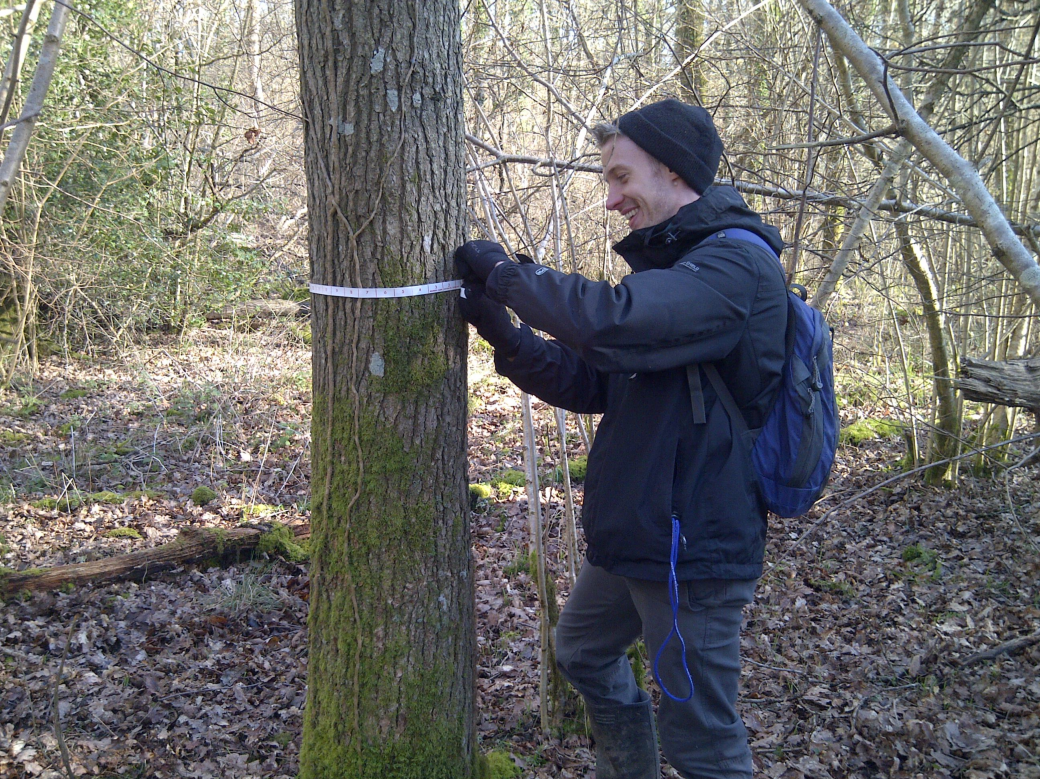
\includegraphics[width=0.8\textwidth]{chapter/chapter4/dbh_me.pdf}
    \caption{Taking diameter at breast height measurements at Alice Holt.} \label{fig:dbh_me}
\end{figure}

\section{Flux tower observations and data processing}

Forest Research provided half-hourly raw flux tower data for the Straits Inclosure from January 1999 to December 2015. These consist of the NEE fluxes and meteorological driving data of temperature, irradiance and atmospheric CO\(_{2}\) concentration for use in the DALEC model. The view from the top of the flux tower in the Straits Inclosure can be seen in Figure~\ref{fig:flux_me}. Forest Research provided this data in the form of multiple excel spreadsheets corresponding to the flux tower measurement record for each year. To prepare this data for use with data assimilation we first had to convert these 16 excel files to one Python readable data file (here we chose NetCDF), this was the further processed. To process the NEE data we first performed \(u^*\) filtering, where any half-hourly flux observation corresponding to a friction velocity of \(0.2~\text{m s}^{-1}\) (this value represents the point at which flux measurements become unreliable and was found by Forest Research) or less were removed from the data set. We then subjected the observations of NEE to quality control procedures similar to those described by \citet{papale2006towards}. For each year of the NEE dataset this procedure involved calculating the standard deviation of both the positive and negative half-hourly observations and then removing any values that were \(\pm 3\) standard deviations away from the yearly positive/negative mean. This was also repeated on a month by month basis. Gap-filling procedures were not applied to the half-hourly NEE dataset so that only true observations were considered for assimilation. To match the time-step of the DALEC model we computed daily NEE observations by taking the mean over the 48 measurements made each day, selecting only days where there was no missing data.  
 

\begin{figure}[ht]
    \centering
    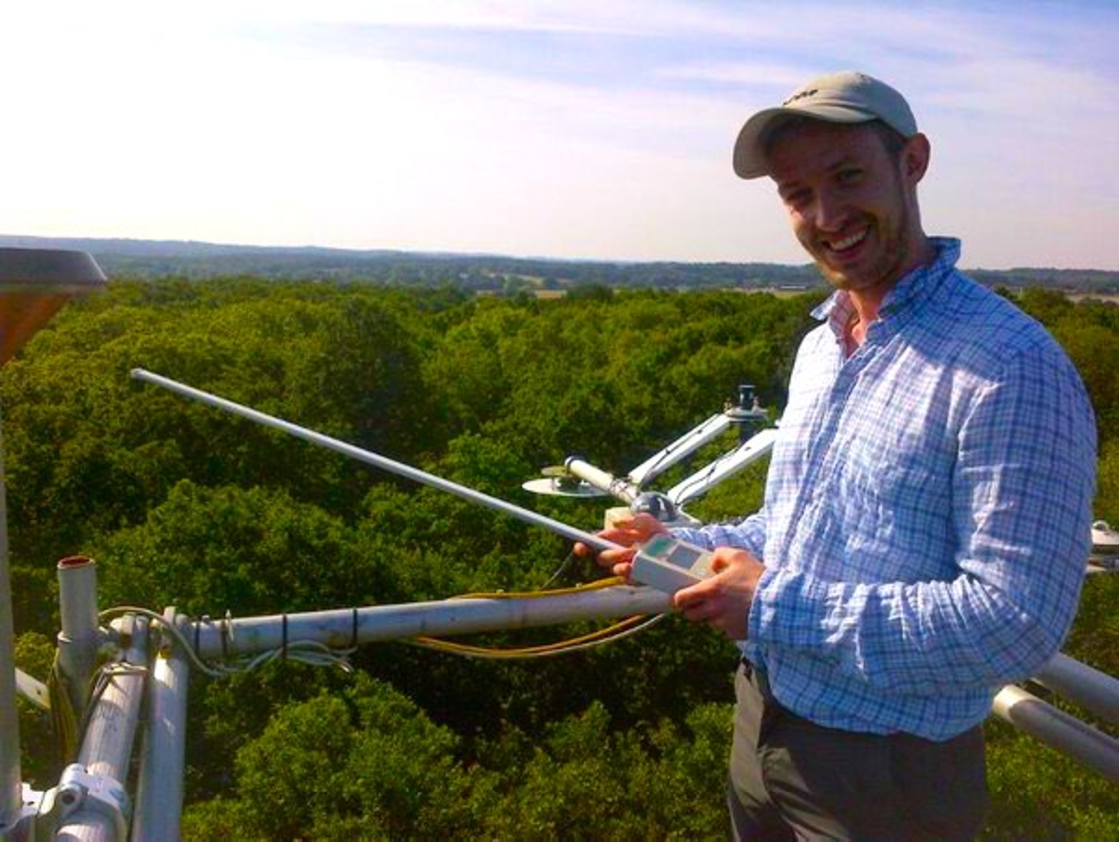
\includegraphics[width=0.8\textwidth]{chapter/chapter4/top_of_flux.pdf}
    \caption{At the top of the Alice Holt flux tower.} \label{fig:flux_me}
\end{figure}



\chapter{Information content in observations relevant to forest carbon balance}
\label{chap:info_con}
%Chapter 5

\section{Introduction}
In data assimilation it is important to understand if the observations available to us provide us with enough information to find a meaningful description of our studied system. Measurements of forest carbon balance are now routinely made in forests across the world using micrometeorological techniques, with many other relevant observations such as leaf area index and standing biomass also available \citep{baldocchi2008turner}. Many efforts have been made to combine this data with models of forest carbon balance using data assimilation techniques in order to improve modelled estimates \citep{zobitz2011primer, fox2009reflex, richardson2010estimating, Quaife2008, Zobitz2014, Niu2014}. Currently, however, the relative levels of information from different data types is not well understood. 

In numerical weather prediction many measures of observation information content have been defined \citep{Cardinali2004, rodgers2000inverse, fisher2003estimation}. These measures can be used to identify how information content might vary both temporally and spatially, when observations are made at different times or in different locations. It is not necessary to have made a physical observation in order to estimate its information content. It is enough to have an accurate estimate to the observation error at the specified time and location. It is therefore possible to use these measures to define target observations or design new observing systems \citep{palmer1998singular, eyre1990information}. Often we are required to know the derivative of our model in order to implement these measures. This can prove difficult to implement. However, techniques such as automatic-differentiation \citep{renaud1997automatic} can reduce the time taken to find the derivative of a model.  

In this chapter we aim to analyse the information content in the observations used for assimilation with the DALEC1 and DALEC2 models of ecosystem carbon balance. We begin by considering the observability of our system given a set of observations. Observability is a mathematical concept from control theory. Applied to data assimilation a system is defined as observable if for a given set of observations we can uniquely define the initial state for our model. This allows us to determine if from current observations used in carbon balance data assimilation, we have enough information to find a unique model state. In practice we include a background term in our assimilation ({\color{red}ref. DA section}) to ensure we can always find a locally unique solution. However, it is informative to show that observations alone provide us with enough information to find a unique solution.

We then consider different information content measures applied to our system in order to show how the information content varies for the different observation types available to us for DALEC1. We then extend these results to the DALEC2 model and investigate how the same set of observations can have a different level of information depending on the type of ecosystem being observed. Using these measures also allows us to consider the effect of including error correlations in our data assimilation algorithm, as explored in section ({\color{red}ref. 1st results chapter}), on the information content in the observations.

\section{Background material}

\subsection{Metolius forest site} \label{sec:oregon}
In this chapter we use meteorological driving data taken from the Metolious forest site, a temperate coniferous forest in Oregon, Northwestern US. The site has been studied extensively \citep{law2001carbon}, and has also been the subject of data assimilation studies \citep{williams2005improved, Quaife2008}. The site has a semi-arid climate with a dominant canopy of ponderosa pine (\textit{Pinus ponderosa}) and an understory of bitterbush (\textit{Purshia tridentata}) and manzanita (\textit{Arctostaphylos patula}) \citep{law2001estimation}. The forest stand was felled in 1978, having previously been a mature forest. It was then allowed to regrow naturally, with some areas of older growth forest still being left post-felling \citep{williams2005improved}.

\subsection{Observability}

Observability is a mathematical concept from control theory. A system is said to be observable if it is possible to determine the state by measuring only the output. The following definition is taken from \citet{barnett1985introduction}: for the linear time varying system defined as,
\begin{align}
\dot{\textbf{x}} &= \textbf{A}(t)\textbf{x}(t) +\textbf{B}(t)\textbf{u}(t) \\
\textbf{y} &= \textbf{C}(t)\textbf{x}(t)
\end{align}
where $\textbf{A}$ is $n \times n$, $\textbf{B}$ is $n \times m$ and $\textbf{C}$ is $r \times n$ is \textit{completely observable} if for any $t_0$ and any initial state $\textbf{x}(t_0) = \textbf{x}_0$ there exists a finite time $t_i > t_0$ such that knowledge of $\textbf{u}(t)$ and $\textbf{y}(t)$ for $t_0 \leq t \leq t_i$ suffices to uniquely determine $\textbf{x}_0$. There is no loss of generality in assuming $\textbf{u}(t)$ is identically zero throughout the whole interval; this is the case for data assimilation. So that in data assimilation our system is \textit{completely observable} if knowledge of the observations $\textbf{y}(t)$ allows us to uniquely determine the initial state $\textbf{x}_0$.

\begin{theorem} \label{thm:observable}
When $\textbf{A}$, $\textbf{B}$ and $\textbf{C}$ are time-invariant the system is completely observable if and only if the $nr \times n$ observability matrix
\begin{equation}
\mathbf{V}=
\begin{pmatrix}
\mathbf{C} \\
\mathbf{C}\mathbf{A}\\
\mathbf{C}\mathbf{A}^{2}\\
\vdots \\
\mathbf{C}\mathbf{A}^{n-1}
\end{pmatrix}
\end{equation}
has rank $n$.
\end{theorem}

This result can be applied to the data assimilation problem \citep{johnson2005singular}, where for 4D-Var the observability matrix corresponds to
\begin{equation}
\hat{\mathbf{H}}=
\begin{pmatrix}
\mathbf{H}_0 \\
\mathbf{H}_1\mathbf{M}_0\\
\vdots \\
\mathbf{H}_N\mathbf{M}_{N,0}
\end{pmatrix} \label{eqn: hmat}
\end{equation}
as defined in section ({\color{red} ref. DA section}). In Appendix B of \citet{zou1992incomplete} it is shown that for the linear data assimilation problem it is possible to obtain a unique analysis state over a specific assimilation window with no background term if the rank of $\hat{\textbf{H}}$ is equal to $n$, the size of $\textbf{x}_0$. For the non-linear data assimilation problem the rank of $\hat{\textbf{H}}$ being equal to $n$ ensures a locally unique analysis can be found without including a background term. In practice the cost function for 4D-Var data assimilation typically contains a background term which regularises the problem and means that we always have a unique solution.

\subsection{Information content measures} \label{sec:IC}%%%%%%%%%%%%%%%%%%%%%% 

In data assimilation we combine prior estimates with observations to improve our knowledge of the state of a system. In this process some observations will have a greater impact on our results than others. Many measures exist for understanding observation impact on the assimilation results.

Information content measures have been used to quantify the different levels of information provided by observations in the development of satellite instruments \citep{stewart2008correlated, engelen2004information} and in operational data assimilation schemes \citep{fisher2003estimation, singh2013practical}. In \citet{Fowler2013} it is discussed that in these operational schemes information content measures have been used for
\begin{itemize}
\item Removing observations with a lesser impact in order to improve the efficiency of the assimilation process \citep{rabier2002channel, singh2013practical, rodgers1998information}.
\item Diagnosing erroneous observations and assumed statistics \citep{desroziers2009posteriori}.
\item Improving data assimilation results by adding observations which theoretically have a high impact. This can mean defining target observations \citep{palmer1998singular} or even designing new observing systems \citep{wahba1985design, eyre1990information}. 
\end{itemize}

For the following measures the data assimilation problem is assumed to be Gaussian with a linear function mapping the state to  observation space (\textbf{H}), following the derivation from \citet{kalnay2003atmospheric} we have,
\begin{equation}
\textbf{x}_{a} = \textbf{x}_{b} + \textbf{K}(\textbf{y} - \textbf{H}\textbf{x}_{b}), \label{eqn:analysis}
\end{equation}
where $\textbf{K}$ is the Kalman gain matrix,
\begin{equation}
\textbf{K} = (\textbf{H}^{T}\textbf{R}^{-1}\textbf{H} + \textbf{B}^{-1})^{-1}\textbf{H}^{T}\textbf{R}^{-1}.
\end{equation}
In order to consider observations over a 4D-Var time window we rewrite equation~\eqref{eqn:analysis} as,
\begin{equation}
\textbf{x}_{a} = \textbf{x}_{b} + \hat{\textbf{K}}(\hat{\textbf{y}} - \hat{\textbf{H}}\textbf{x}_{b}),
\end{equation}
using the defined matrices in section ({\color{red} ref DA section}), with $\hat{\textbf{K}} = (\hat{\textbf{H}}^{T}\hat{\textbf{R}}^{-1}\hat{\textbf{H}} + \textbf{B}^{-1})^{-1}\hat{\textbf{H}}^{T}\hat{\textbf{R}}^{-1}.$ 

Making the assumption of a linear and Gaussian data assimilation problem is clearly a limitation. These measures are therefore limited to a period where the forecast model remains reasonably linear. The implications of assuming Gaussian error statistics are discussed in \citet{Fowler2013}.

%\citep{fisher2003estimation} **Reference about SIC and DFS being used in operational atmospheric DA.

%\citep{singh2013practical} **Ref about using fischer mat, dfs and SIC for data pruning to produce similar results.

\subsubsection{Sensitivity of analysis to observations} \label{sec:inf_mat}

The influence matrix measures the sensitivity of the analysis in observation space to the observations \citep{Cardinali2004} and is defined by,
\begin{equation}
\textbf{S} = \frac{\partial \textbf{H}\textbf{x}_{a}}{\partial \textbf{y}}. \label{eqn:inf_mat}
\end{equation}
From equation~\eqref{eqn:analysis} we see that,
\begin{equation}
\begin{split}
\textbf{S} &= \frac{\partial \textbf{H}(\textbf{x}_{b} + \textbf{K}(\textbf{y} - \textbf{H}\textbf{x}_{b}))}{\partial \textbf{y}} \\
	       &= \textbf{K}^{T}\textbf{H}^{T},
\end{split}
\end{equation}
here $\textbf{S}$ will be a $p \times p$ matrix, where $p$ is the number of observations. The diagonal elements of $\textbf{S}$ are $\textbf{S}_{i,i} = \frac{\partial (\textbf{H}\textbf{x}_{a})_{i}}{\partial \textbf{y}_{i}}$ and represent the `self-sensitivity' of the $i^{th}$ modelled observation to the $i^{th}$ observation. The off-diagonal elements of $\textbf{S}$ represent the `cross-sensitivity' and are given by $\textbf{S}_{i,j} = \frac{\partial (\textbf{H}\textbf{x}_{a})_{i}}{\partial \textbf{y}_{j}}$. If we wish to consider the influence matrix for observations over a 4D-Var time window we can re-write equation~\eqref{eqn:inf_mat} as,
\begin{equation}
\textbf{S} = \frac{\partial \hat{\textbf{H}}\textbf{x}_{a}}{\partial \hat{\textbf{y}}} = \hat{\textbf{K}}^{T}\hat{\textbf{H}}^{T}. \label{eqn:4dinf_mat}
\end{equation}
The Kalman gain matrix $\hat{\textbf{K}}$ can be re-written as,
\begin{equation}
\hat{\textbf{K}} = \textbf{A}\hat{\textbf{H}}^{T}\hat{\textbf{R}}^{-1}, \label{eqn:analysis_kgain}
\end{equation}
where $\textbf{A}$ is the analysis error covariance,
\begin{equation}
\textbf{A} = (\hat{\textbf{H}}^{T}\hat{\textbf{R}}^{-1}\hat{\textbf{H}} + \textbf{B}^{-1})^{-1}.
\end{equation}
Inserting equation~\eqref{eqn:analysis_kgain} into \eqref{eqn:4dinf_mat} we find,
 \begin{equation}
 \textbf{S} = \hat{\textbf{R}}^{-1}\hat{\textbf{H}}\textbf{A}\hat{\textbf{H}}^{T}.
 \end{equation}
We can therefore see the sensitivity of the analysis to observations is inversely proportional to the observation error and proportional to the analysis error. This means that the most influential observations are those with the smallest error variance providing information about regions of state space with the largest prior error \citep{Cardinali2004}. It is possible to identify the observations that have the greatest influence over the length of the window by summing the absolute values of the columns of the influence matrix.

\subsubsection{Degrees of freedom for signal} \label{DFSintro}%%%%%%%%%%%%%%%%%%%%%%

The degrees of freedom for signal ($dfs$) indicates the number of elements of the state that have been measured by the observations. If we consider a state vector $\textbf{x}$ with $n$ elements (or $n$ degrees of freedom) then the maximum value the $dfs$ could obtain would be $n$, in this case all elements of the state would have been measured. Conversely if $dfs = 0$ then no elements of the state would have been measured by our observations \citep{Fowler2013}.

For a symmetric positive definite prior and posterior error covariance matrices $\bf{B}$ and $\bf{A}$, we can define the degrees of freedom for signal by means of a transform $\textbf{L}$ that reduces the prior error covariance matrix, $\textbf{B}$ to the $n \times n$ identity \citep{fisher2003estimation}. Each diagonal element of the transformed matrix $\textbf{B}$ then corresponds to a single degree of freedom with the trace being equal to $n$, the total degrees of freedom. 

The transform $\textbf{L}$ can also be represented by $\textbf{Q}^{T}\textbf{L}$, where $\textbf{Q}$ is an orthogonal matrix. So that $\textbf{Q}^{T}\textbf{L}\textbf{B}\textbf{L}^{T}\textbf{Q} = \textbf{Q}^{T}\textbf{Q} = \textbf{I}_{n \times n}$. By defining $\textbf{Q}$ to be the matrix of the eigenvectors of $\textbf{L}\textbf{A}\textbf{L}^{T}$, we reduce $\textbf{B}$ to the identity and $\textbf{L}\textbf{A}\textbf{L}^{T}$ to the diagonal matrix of its eigenvalues, $\bm{\Lambda}$. The eigenvalues $\lambda_{i}$ of $\textbf{L}\textbf{A}\textbf{L}^{T}$ can be interpreted as the fractional reduction in uncertainty for the $n$ state members. If an eigenvalue is close to zero the corresponding state member has been well observed, if it is close to one the corresponding state member has not been constrained by the assimilated observations \citep{stewart2008correlated}. We then define the degrees of freedom for signal as,
\begin{equation}
\begin{split}
dfs & = \text{trace}(\textbf{Q}^{T}\textbf{L}\textbf{B}\textbf{L}^{T}\textbf{Q} - \textbf{Q}^{T}\textbf{L}\textbf{A}\textbf{L}^{T}\textbf{Q}) \\
       & = \text{trace}(\mathbf{I}_{n\times n} - \bm{\Lambda}) \\
       & = n - \text{trace}(\bm{\Lambda}) \\
       & = n - \text{trace}(\textbf{L}\textbf{A}\textbf{L}^{T}) \\
       & = n - \text{trace}(\mathbf{B}^{-1}\mathbf{A}). \label{eqn:dfs}
\end{split}
\end{equation}
In \citet{rodgers2000inverse} it is shown that the $dfs$ can also be calculated as the trace of the influence matrix $\textbf{S}$ (defined in section~\ref{sec:inf_mat}) with,
\begin{equation}
dfs = \text{trace}(\textbf{S}) = \sum_{i} \lambda_{i},
\end{equation}
where $\lambda_{i}$ is the $i^{th}$ eigenvalue of $\textbf{S}$.

\subsubsection{Shannon information content}%%%%%%%%%%%%%%%%%%%%%%

Shannon Information Content (SIC) is a measure of the reduction in entropy (uncertainty) given a set of observations. When a measurement is made, the entropy or uncertainty in our state decreases. The SIC of an observation is a measure of the factor by which the uncertainty decreases \citep{cover1991elements}. We can define this using the prior, $p(\textbf{x})$, and posterior, $p(\textbf{x}|\textbf{y})$, distributions. From \citet{rodgers2000inverse}, for the Gaussian case SIC unsprisingly becomes a function of the prior and posterior error covariance matrices with,
\begin{equation}
\text{SIC}=\frac{1}{2}\text{ln}\frac{\begin{vmatrix} \bf{B} \end{vmatrix}}{\begin{vmatrix} \bf{A} \end{vmatrix}}. \label{eqn:sic}
\end{equation}
The SIC can also be defined in terms of the eigenvalues of the influence matrix $\textbf{S}$ with,
\begin{equation}
\text{SIC} = -\frac{1}{2} \sum_{i} ln | 1 - \lambda_{i} |
\end{equation}
where $\lambda_{i}$ is the $i^{th}$ eigenvalue of $\textbf{S}$. In \citet{eyre1990information} using SIC is shown to be beneficial over solely measuring the change in error variances before and after assimilation as the SIC also uses information about the change in error covariances. This is also true for the $dfs$.   

\section{Results}

\subsection{DALEC1 observability} \label{sec:D1observability}

DALEC1 is the original version of the DALEC2 model introduced in section ({\color{red}ref. D2 section}). At the start of the PhD project work was undertaken with DALEC1 before the DALEC2 model was released. The version of DALEC1 used was an evergreen only model; further details of the model can be found in section ({\color{red}ref. D1 section}) and \citet{williams2005improved}. 

We initially consider observability of the DALEC1 state estimation system. DALEC1 is a smaller model and allows us to understand the concept of observability before moving onto work with the more complicated DALEC2 joint state and parameter estimation system. DALEC1 was implemented in a 4D-Var data assimilation scheme for state estimation, with the tangent linear model being computed analytically. Using this analytic implementation of the tangent linear model we can compute the observability of the model for differing sets of observations. We have the tangent linear model,
\begin{multline}
\mathbf{M}_{i} = \frac{\partial \textbf{m}_{i-1\rightarrow i}(\textbf{x}_{i})}{\partial \textbf{x}_{i}} = 
\\ \begin{pmatrix}  
(1-\theta_{fol})+f_{fol}(1-f_{auto})\zeta^i & 0 & 0 & 0 & 0 \\
f_{roo}(1-f_{fol})(1-f_{auto})\zeta^i & (1-\theta_{roo}) & 0 & 0 & 0 \\
(1-f_{roo})(1-f_{fol})(1-f_{auto})\zeta^i & 0 & (1-\theta_{woo}) & 0 & 0 \\
\theta_{fol} & \theta_{roo} & 0 & (1-(\theta_{min}+\theta_{lit})\chi^{i-1}) & 0 \\
0 & 0 & \theta_{woo} & \theta_{min}\chi^{i-1} & (1-\theta_{som}\chi^{i-1}) \\
\end{pmatrix}, \label{eqn:linmod}
\end{multline}
where \(\textbf{x}_{i}=(C_{fol}^{i}, C_{roo}^{i}, C_{woo}^{i}, C_{lit}^{i}, C_{som}^{i})^{T}\), \(\zeta^i = \partial GPP^{i}(C_{fol}^{i-1}, \Psi)/\partial C_{fol}^{i-1}\) and \(\chi^{i-1}=e^{\Theta T^{i-1}}\) with the parameters and symbols having the same meaning as in section ({\color{red}ref. D2 section}). 

We can use the linearised model with the linearised observation operator $\textbf{H}_{i}$ to form the matrix in equation~\eqref{eqn: hmat} and compute the observability for a specific set of observations over a finite window. We will need at least 5 observations of any type for the system to be observable as the state $\textbf{x}_0$ is of size 5 in the DALEC1 state estimation case. We first consider the observability for 5 observations of LAI. For DALEC1 LAI takes the form
\begin{equation}
LAI^{i} = \frac{C_{fol}^{i}}{c_{lma}}.
\end{equation}
We then have the linearised observation operator
\begin{equation}
\textbf{H}_{i} = \frac{\partial LAI^{i}}{\partial \textbf{x}_{i}} =
\begin{pmatrix}
\frac{1}{c_{lma}} & 0 & 0 & 0 & 0
\end{pmatrix}.
\end{equation}
Using the linearised observation operator and the linear model from equation~\eqref{eqn:linmod} we can compute $\hat{\textbf{H}}$ for 5 observations of LAI on consecutive time steps
\begin{multline}
\hat{\mathbf{H}} =
\begin{pmatrix}
\mathbf{H}_0 \\
\mathbf{H}_1\mathbf{M}_0 \\
\vdots \\
\mathbf{H}_{4}\mathbf{M}_{3,0}
\end{pmatrix}
= \begin{pmatrix}
\frac{1}{c_{lma}} & 0 & 0 & 0 & 0 \\
\frac{1}{c_{lma}}((1-\theta_{fol})+f_{fol}(1-f_{auto})\zeta^0) & 0 & 0 & 0 & 0 \\
\frac{1}{c_{lma}}\prod_{i=0}^{1}((1-\theta_{fol})+f_{fol}(1-f_{auto})\zeta^i) & 0 & 0 & 0 & 0 \\
\frac{1}{c_{lma}}\prod_{i=0}^{2}((1-\theta_{fol})+f_{fol}(1-f_{auto})\zeta^i) & 0 & 0 & 0 & 0 \\
\frac{1}{c_{lma}}\prod_{i=0}^{3}((1-\theta_{fol})+f_{fol}(1-f_{auto})\zeta^i) & 0 & 0 & 0 & 0
\end{pmatrix},
\end{multline}
so that no matter how many observations of LAI we add, our system will not be observable as the rows of $\hat{\textbf{H}}$ are all linearly dependant, so that $\hat{\textbf{H}}$ in this case has rank 1. We can repeat this for different observations to see for which observation types our system is observable. 

\begin{figure}[ht]
    \centering
    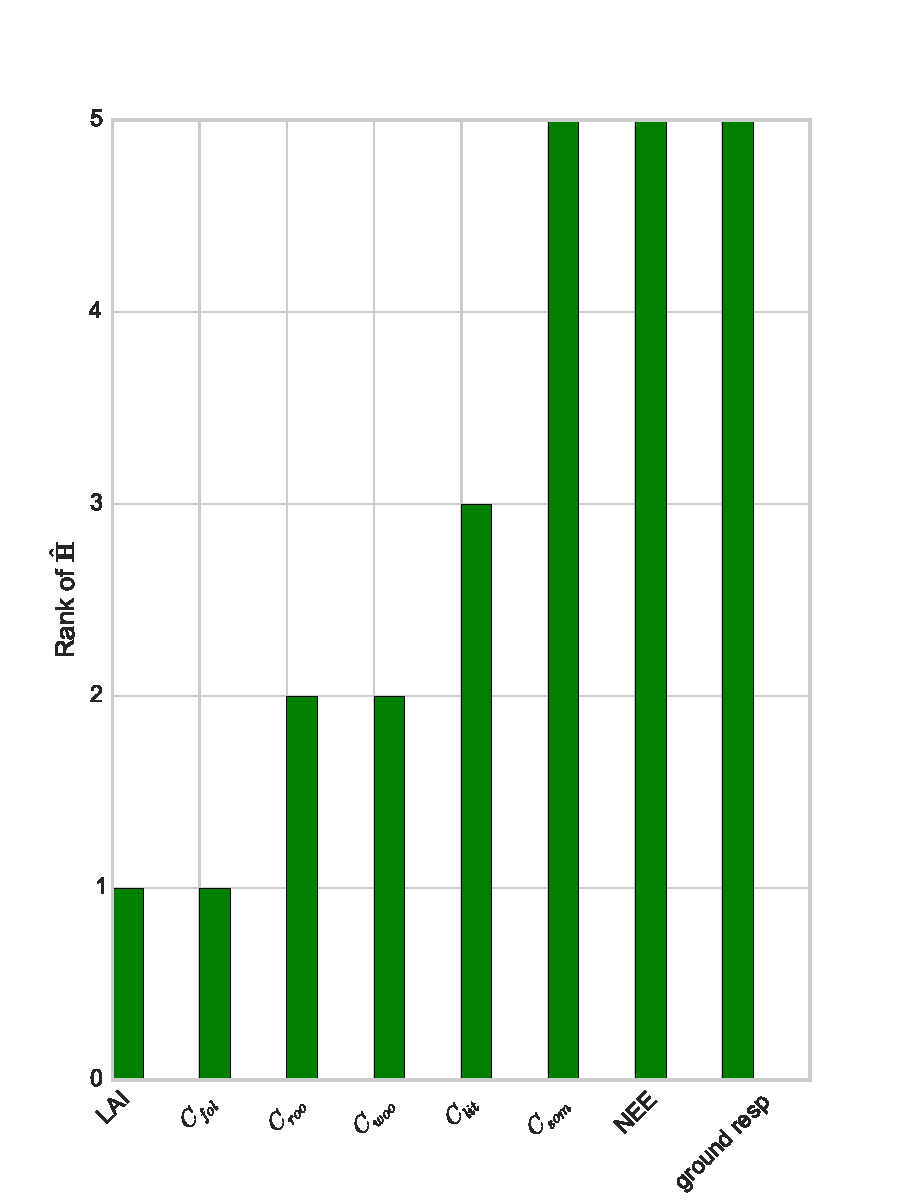
\includegraphics[width=0.5\textwidth]{chapter/chapter5/dalec1_obsrank.pdf}
    \caption{Rank of the observability matrix $\hat{\textbf{H}}$ for 5 observations of different types. The ranks shown here are computed analytically using SymPy \citep{Joyner:2012:OSC:2110170.2110185}.}
    \label{fig:D1_observability}
\end{figure}

From figure~\ref{fig:D1_observability} we can see that our system is observable for 5 observations of the soil and organic matter carbon pool $C_{som}$. In figure~\ref{fig:D1_observability} we have shown results for the rank of  $\hat{\textbf{H}}$ when we have 5 observations in each case; this has also been tested with increasing numbers of observations being added to the system with the results from figure~\ref{fig:D1_observability} remaining unchanged. 

The system being observable for observations of $C_{som}$ physically makes sense as all the carbon in the system that is not respired to the atmosphere eventually ends up in the soil and organic matter carbon pool, $C_{som}$, so that by taking observations of this pool we observe all the others. In a similar way $\hat{\textbf{H}}$ is also full rank for observations of NEE and ground respiration. We can see from the form of these observations in DALEC1 that they both contain indirect observations of $C_{som}$ with NEE taking the form
\begin{equation}
NEE^{i}=-(1-f_{auto})GPP^{i}(C_{fol}^{i-1}, \Psi) + \theta_{lit}C_{lit} e^{\Theta T^{i}} + \theta_{som}C_{som} e^{\Theta T^{i}} \label{eqn: D1_nee}
\end{equation}
with a corresponding linearised observation operator
\begin{equation}
\textbf{H}_{i} = \frac{\partial NEE^{i}}{\partial \textbf{x}_{i}} =
\begin{pmatrix}
-(1-f_{auto})\zeta^i & 0 & 0 & \theta_{lit} e^{\Theta T^{i}} & \theta_{som} e^{\Theta T^{i}}
\end{pmatrix},
\end{equation}
and for ground respiration
\begin{equation}
G_{resp}^{i}=\frac{1}{3}f_{auto}GPP^{i}(C_{fol}^{i-1}, \Psi) + \theta_{lit}C_{lit} e^{\Theta T^{i}} + \theta_{som}C_{som} e^{\Theta T^{i}} \label{neeeqn}
\end{equation}
(here we have assumed the fraction of total autotrophic respiration from below ground to be $\frac{1}{3}$) with a corresponding linearised observation operator
\begin{equation}
\textbf{H}_{i} = \frac{\partial G_{resp}^{i}}{\partial \textbf{x}_{i}} =
\begin{pmatrix}
\frac{1}{3}f_{auto}\zeta^i & 0 & 0 & \theta_{lit} e^{\Theta T^{i}} & \theta_{som} e^{\Theta T^{i}}
\end{pmatrix}.
\end{equation}
At flux tower sites NEE is the most observed quantity, these results give us confidence that we can construct a unique solution when working with flux tower data. We will further explore the concept of observability for the joint parameter and state estimation case with DALEC2 in section~\ref{sec: D2_observability}. 

%\FloatBarrier
\subsection{DALEC2 observability} \label{sec: D2_observability}

For DALEC2 we perform joint parameter and state estimation and have an augmented state of size $n = 23$. The augmented state is made up of the 6 carbon pool state members and 17 model parameters as described in section~({\color{red}ref. D2 section}). As we are also estimating the parameters of DALEC2 the concept of observability for our system is closely linked to the concept of identifiability \citep{navon1998practical}. A system is identifiable if given observations of the state variables and knowledge of the model dynamics it is possible to obtain a unique deterministic set of model parameter values \citep{ljung1998system}. If a model parameter is not observable it will not be identifiable \citep{Jacquez1985}. It is therefore useful to compute the observability of the DALEC2 joint parameter and state estimation system.

We compute observability in the same way as in section~\ref{sec:D1observability} by finding the rank of $\hat{\textbf{H}}$ for a given set of observations. For the state and parameter estimation case we cannot compute the observability of the system analytically, it is therefore important to check that the numerical calculation of the rank of $\hat{\textbf{H}}$ for DALEC1 is equal to the rank when calculated analytically. This will give us confidence that our implementation of the numeric rank is correct for DALEC2 when applied to a well-conditioned problem as the implementation is the same in both cases. We have tested our numeric implementation for the state estimation case with DALEC1 and find the same results for the rank of $\hat{\textbf{H}}$ as for the analytic case, as shown in table~\ref{table: a_n_h_D1}. We calculate the rank of the $\hat{\textbf{H}}$ matrix using a singular value decomposition (SVD) which can have issues if the condition number of $\hat{\textbf{H}}$ is large \citep{Paige1981}. This is a problem we encounter in the DALEC2 case when trying to calculate the rank of $\hat{\textbf{H}}$ directly.  

\begin{table}[ht] 
\begin{center}
	\begin{tabular}{| l | l | l | l}
	\hline
	Observation & Rank of $\hat{\textbf{H}}$ (numeric) & Rank of $\hat{\textbf{H}}$ (analytic) \\ \hline
	LAI & 1 & 1 \\ \hline
	$C_{fol}$ & 1 & 1  \\ \hline
	$C_{roo}$ & 2 & 2 \\ \hline
	$C_{woo}$ & 2 & 2 \\ \hline
	$C_{lit}$ & 3 & 3 \\ \hline
	$C_{som}$ & 5 & 5 \\ \hline
	NEE & 5 & 5 \\ \hline
	$G_{resp}$ & 5 & 5 \\  
	\hline
	\end{tabular}
	\caption{Rank of $\hat{\textbf{H}}$ for 5 observations of different types for both numeric and analytic implementations with DALEC1.}
	\label{table: a_n_h_D1}
\end{center} 
\end{table}


\begin{figure}[ht]
    \centering
    \begin{subfigure}[b]{0.4\textwidth}
        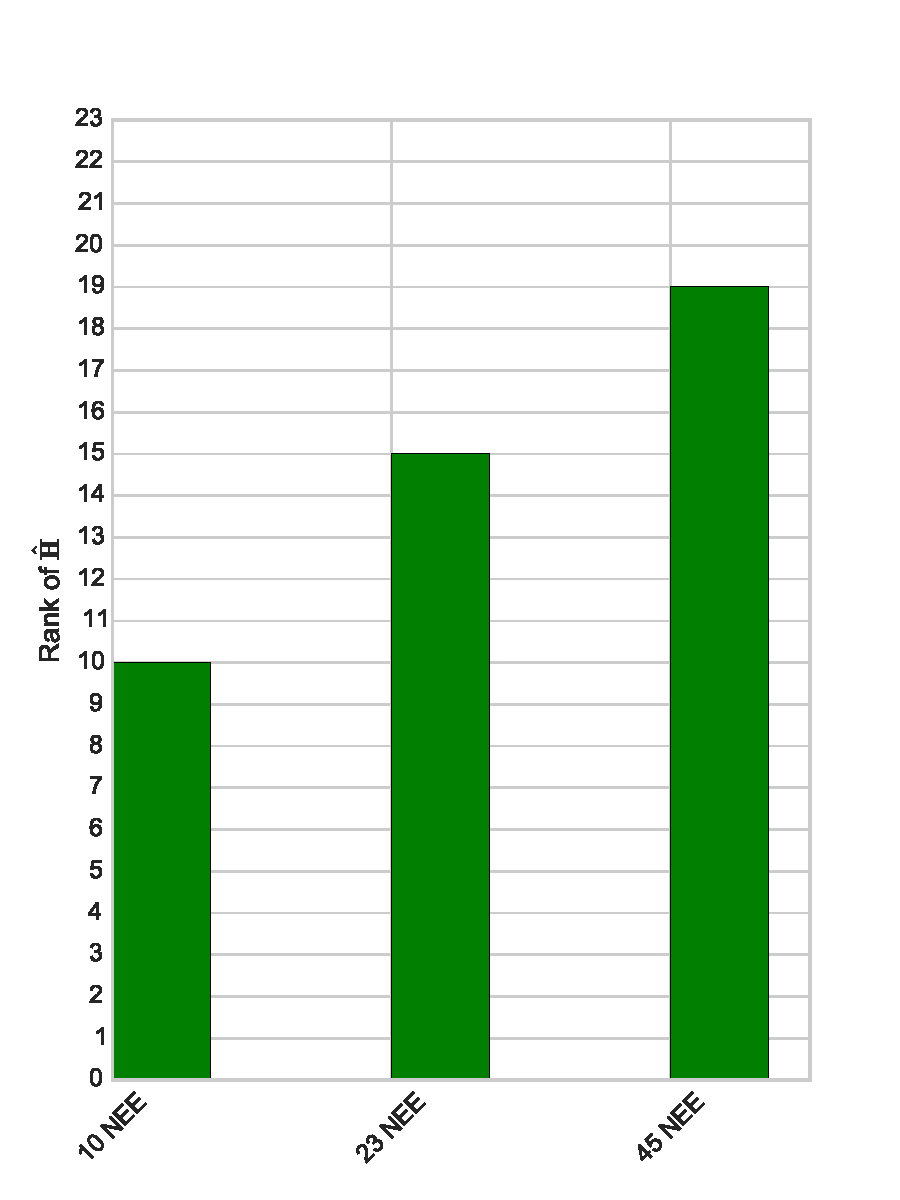
\includegraphics[width=\textwidth]{chapter/chapter5/dalec2_obsrank.pdf}
        \caption{Rank of $\hat{\textbf{H}}$}
        \label{fig:D2_observabilityrank}
    \end{subfigure}%
    \begin{subfigure}[b]{0.4\textwidth}
        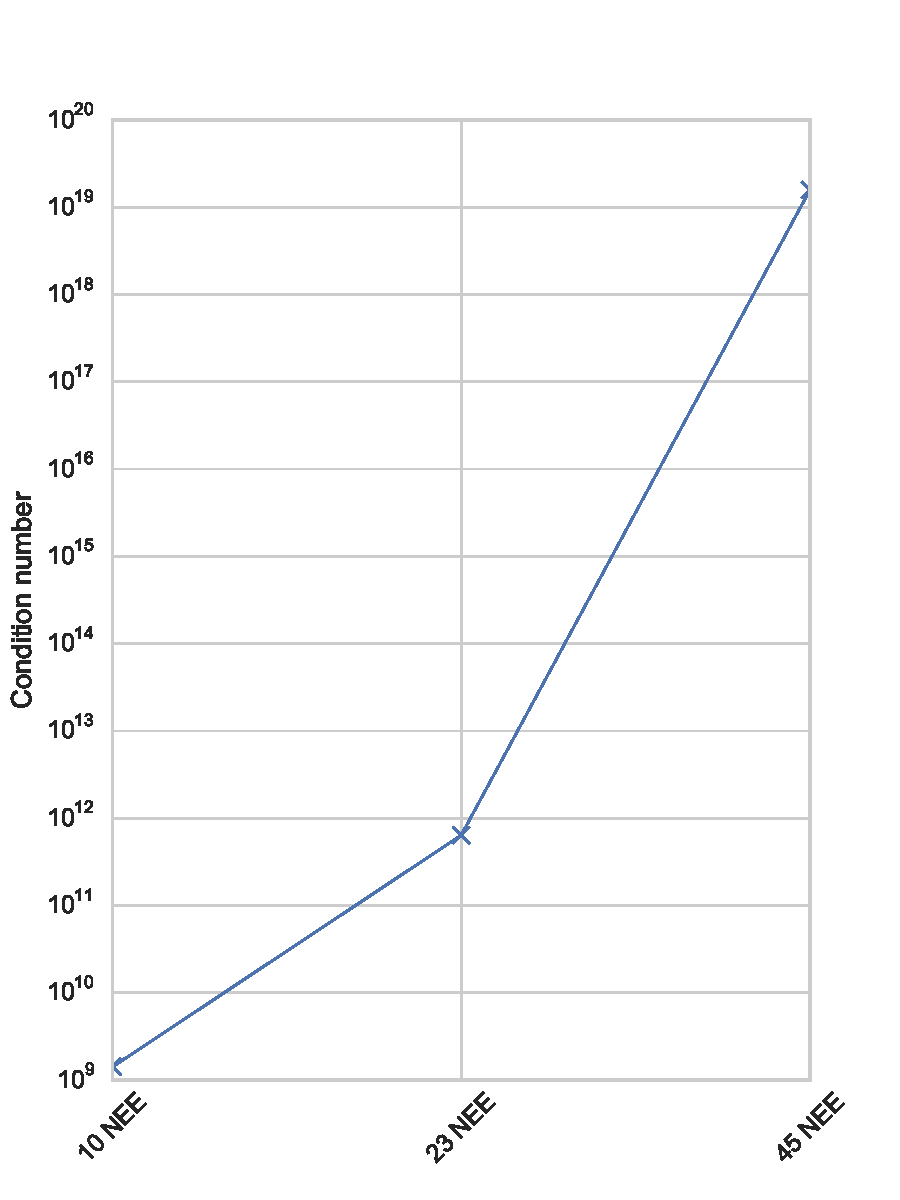
\includegraphics[width=\textwidth]{chapter/chapter5/dalec2_obsrankcond.pdf}
        \caption{Condition number of $\hat{\textbf{H}}$}
        \label{fig:D2_observabilitycond}
    \end{subfigure}
    \caption{Observability of DALEC2 for $\hat{\textbf{H}}$ with an increasing number of NEE observations displayed alongside the condition number for the $\hat{\textbf{H}}$ matrices.}
    \label{fig:D2_observability}
\end{figure}

Figure~\ref{fig:D2_observability} highlights the problems we have calculating the rank of the $\hat{\textbf{H}}$ matrix for the DALEC2 joint parameter and state estimation case. In figure~\ref{fig:D2_observabilityrank} we see that for 23 observations of NEE our system is unobservable as we have a rank deficient $\hat{\textbf{H}}$. However, we cannot trust the rank calculation of $\hat{\textbf{H}}$ in this case. Figure~\ref{fig:D2_observabilitycond} shows that for 23 observations of NEE, $\hat{\textbf{H}}$ has a condition number in the order of $10^{19}$. The condition number of a matrix corresponds to the ratio of the largest to the smallest singular values. A condition number of this size means that we have very small singular values. In the calculation of the rank of a matrix using an SVD we define the rank to be the number of singular values greater than the threshold \texttt{ tol = max(S) * max(n, m) * eps } \citep{press2007numerical}, where \texttt{S} is the vector of singular values, \texttt{n} and \texttt{m} are the rows and columns of the matrix whose rank we wish to calculate and \texttt{eps} is the machine accuracy for the datatype of \texttt{S} (In this case a double-precision float with \texttt{eps = 2.22e-16}). For 23 observations of NEE, $\hat{\textbf{H}}$ is classed as being rank deficient as \texttt{tol = 1.02e-10} and the three smallest singular values of $\hat{\textbf{H}}$ are \texttt{[1.39e-11, 7.84e-15, 1.46e-15]} but here we are working past the accuracy of the computer and so cannot have confidence that $\hat{\textbf{H}}$ is rank deficient in this case.

\begin{figure}[ht]
    \centering
    \begin{subfigure}[b]{0.4\textwidth}
        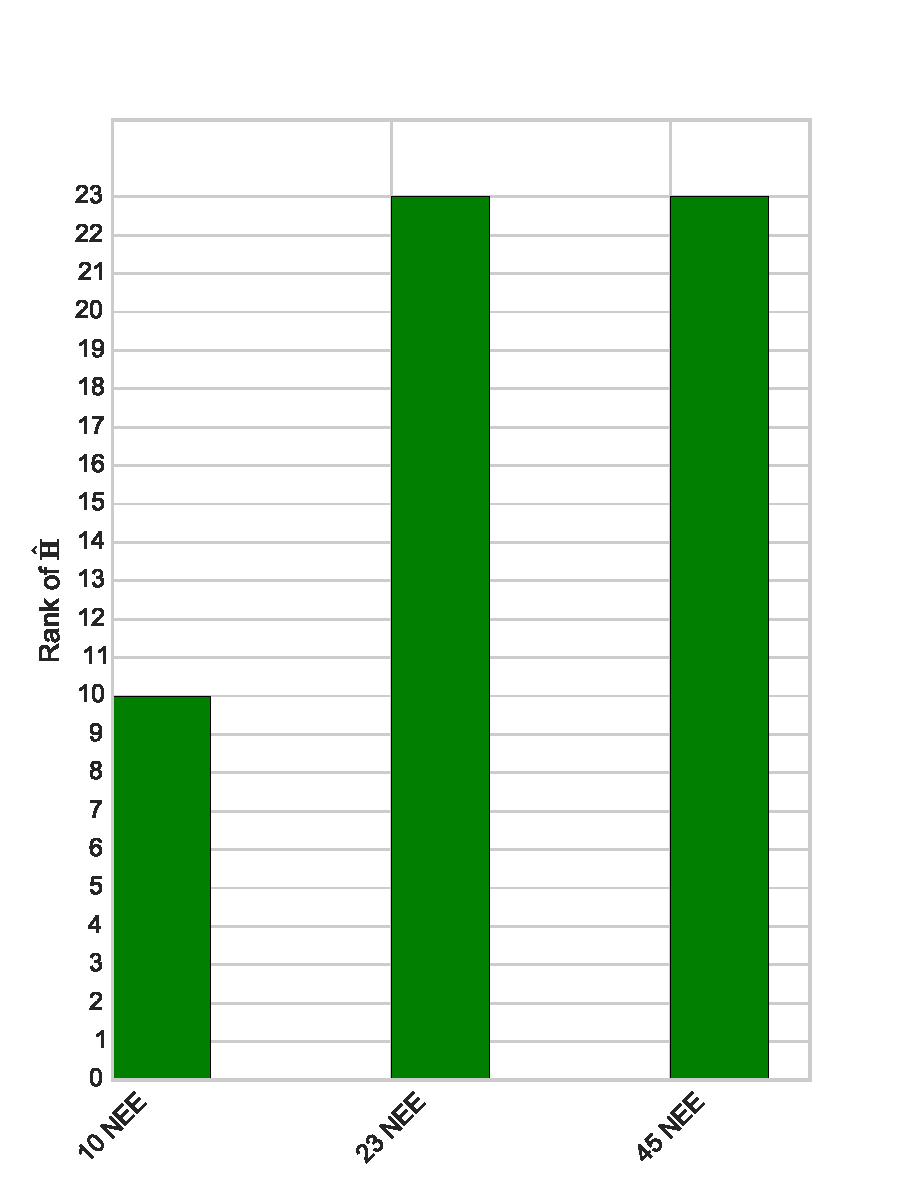
\includegraphics[width=\textwidth]{chapter/chapter5/dalec2_obsrankcvt.pdf}
        \caption{Rank of $\hat{\textbf{R}}^{-1/2}\hat{\textbf{H}}\textbf{D}^{1/2}$}
        \label{fig:D2_observailityrankcvt}
    \end{subfigure}
    \begin{subfigure}[b]{0.4\textwidth}
        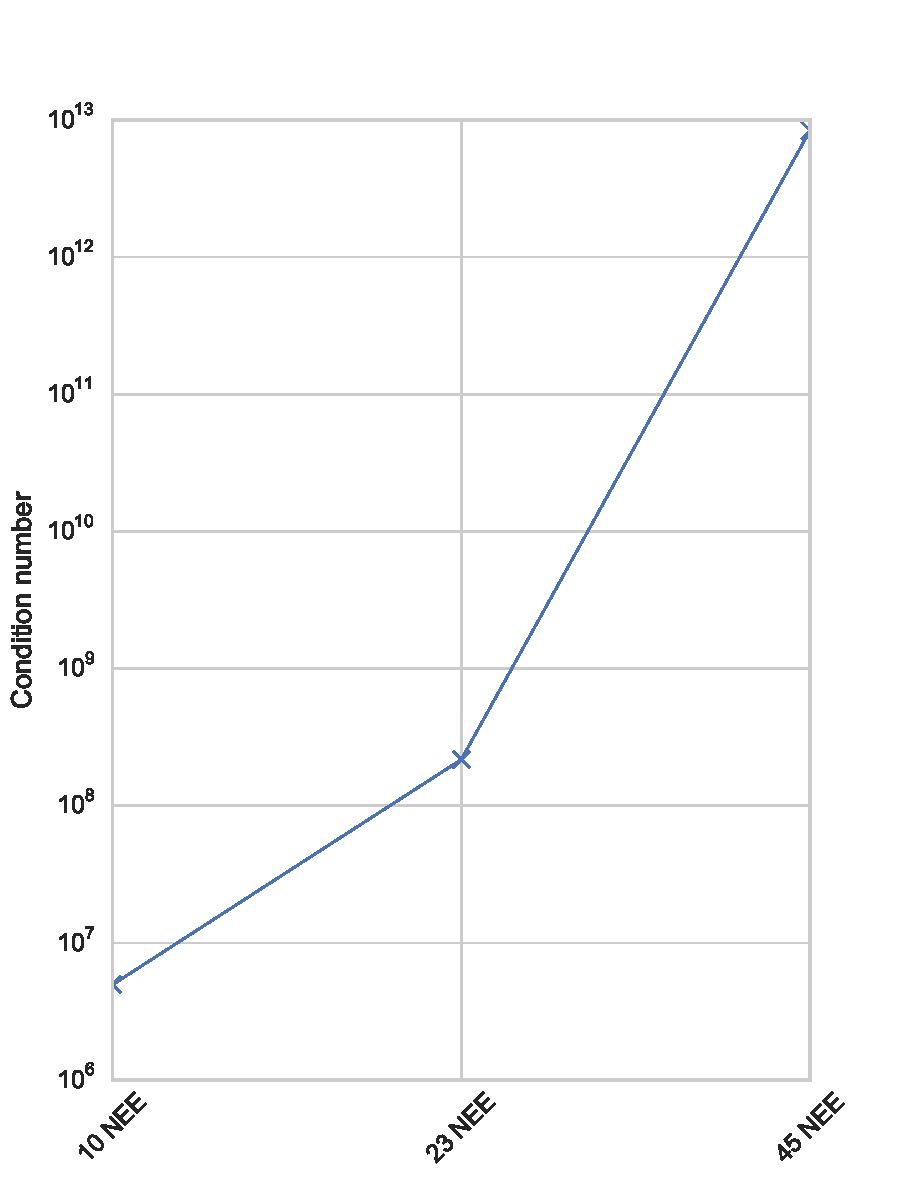
\includegraphics[width=\textwidth]{chapter/chapter5/dalec2_obsrankcvtcond.pdf}
        \caption{Condition number of $\hat{\textbf{R}}^{-1/2}\hat{\textbf{H}}\textbf{D}^{1/2}$}
        \label{fig:D2_observabilitycondcvt}
    \end{subfigure}
    \caption{Observability of the CVT DALEC2 for $\hat{\textbf{R}}^{-1/2}\hat{\textbf{H}}\textbf{D}^{1/2}$ with an increasing number of NEE observations displayed alongside the condition number for the $\hat{\textbf{R}}^{-1/2}\hat{\textbf{H}}\textbf{D}^{1/2}$ matrices.}
    \label{fig:D2_cvtobservability}
\end{figure}

In order to address the problem of ill-conditioning of the $\hat{\textbf{H}}$ matrix we can instead calculate the rank of the control variable transform observability matrix, $\hat{\textbf{R}}^{-1/2}\hat{\textbf{H}}\textbf{D}^{1/2}$, where the symbols have the same meaning as in section ({\color{red}ref DA CVT section, $\textbf{D} = diag\{\textbf{B}\}$}). The rank of $\hat{\textbf{R}}^{-1/2}\hat{\textbf{H}}\textbf{D}^{1/2}$ and $\hat{\textbf{H}}$ are the same since $\hat{\textbf{R}}$ and $\textbf{D}$ are both full rank matrices. The results using this new better conditioned matrix are shown in Figure~\ref{fig:D2_cvtobservability}. From Figure~\ref{fig:D2_observabilitycondcvt} we can see this matrix is much better conditioned than $\hat{\textbf{H}}$, and for 23 observations of NEE we now have an observable system. Although the condition numbers here are still large we can have more confidence in these results as we are working within the precision of the computer.

\subsubsection{Observability for observations randomly distributed through time}

In the previous experiments we have considered increasing numbers of NEE observations taken on adjacent days. It is also useful to consider the observability of the system when we have a number of observations randomly distributed throughout a time window. This is more consistent with what we expect from the real data we have to work with.  

\begin{figure}[ht]
    \centering
    \begin{subfigure}[b]{0.4\textwidth}
        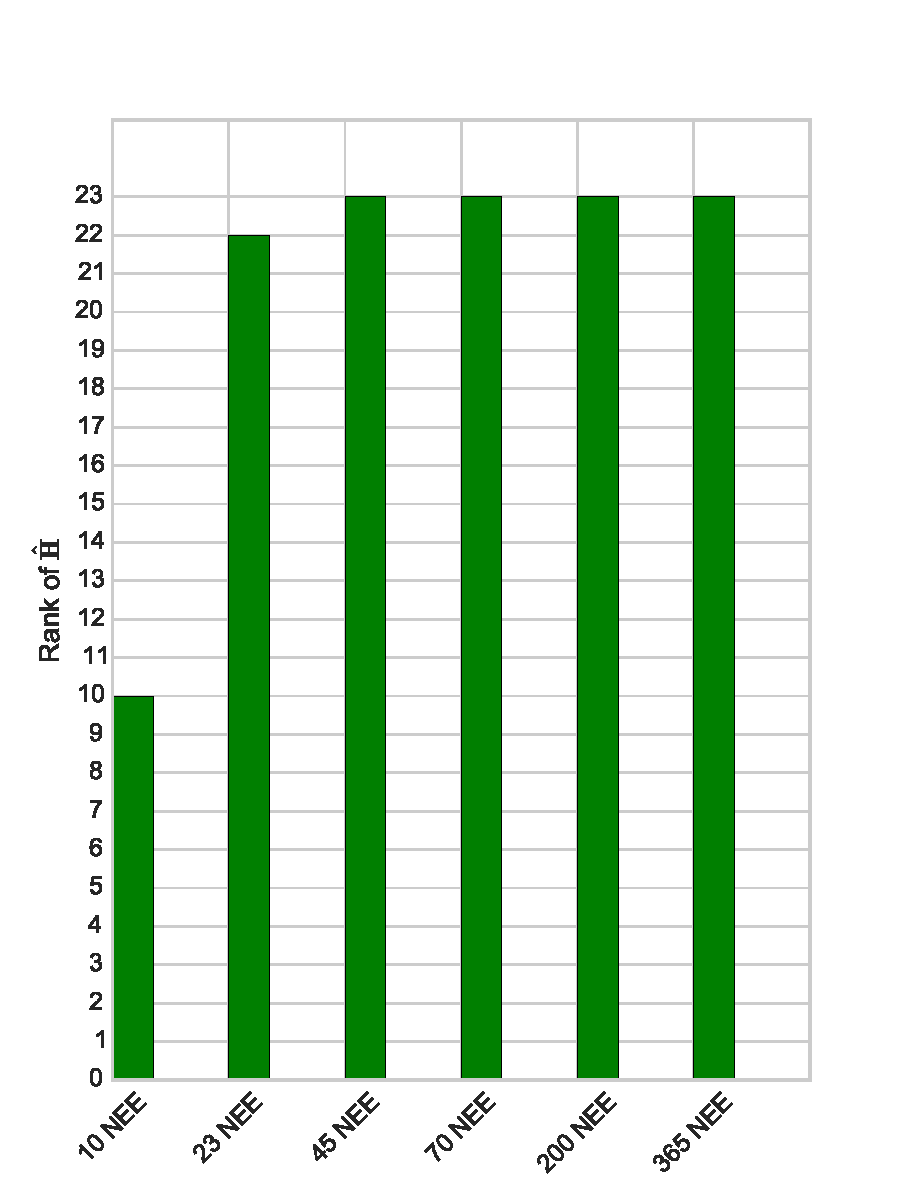
\includegraphics[width=\textwidth]{chapter/chapter5/dalec2_obsrankwind.pdf}
        \caption{Rank of $\hat{\textbf{H}}$}
        \label{fig:D2_observailityrankwind}
    \end{subfigure}
    \begin{subfigure}[b]{0.4\textwidth}
        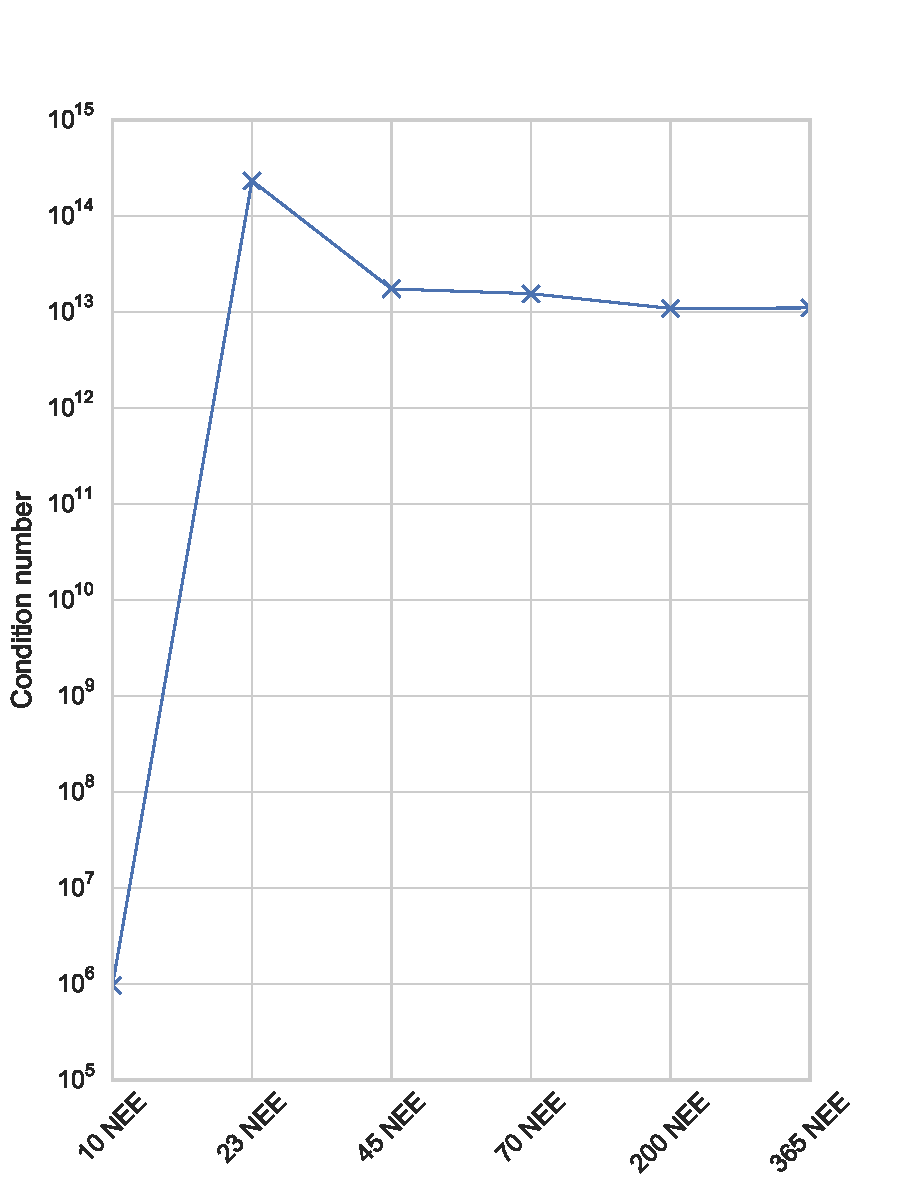
\includegraphics[width=\textwidth]{chapter/chapter5/dalec2_obsrankcondwind.pdf}
        \caption{Condition number of $\hat{\textbf{H}}$}
        \label{fig:D2_observabilitycondwind}
    \end{subfigure}
    \caption{Observability of DALEC2 for a $\hat{\textbf{H}}$ with an increasing number of NEE observations randomly distributed through a 1 year assimilation window (left). Condition number for the $\hat{\textbf{H}}$ matrices (right).}
    \label{fig:D2_observabilitywind}
\end{figure}

Figure~\ref{fig:D2_observabilitywind} shows the observability for an increasing number of observations distributed through a 1 year assimilation window. I this case we are using the matrix $\hat{\textbf{H}}$ and not the CVT observability matrix. In figure~\ref{fig:D2_observabilitywind} we see that having the observations randomly distributed throughout a 1 year assimilation window has improved the conditioning of $\hat{\textbf{H}}$ in comparison to figure~\ref{fig:D2_observability}. This is due to the observations being randomly distributed rather than adjacent. The rows of $\hat{\textbf{H}}$ are more distinct when being evolved to different times in the year by the tangent linear model rather than evolved to adjacent days only. However, we still have a rank deficient $\hat{\textbf{H}}$ for the 23 NEE observation case. From figure~\ref{fig:D2_observabilitycondwind} we see that this is the case where the condition number peaks. As we add more randomly distributed observations the condition number of $\hat{\textbf{H}}$ is reduced by an order of $10^{2}$ and we have a full rank $\hat{\textbf{H}}$. 

In figure~\ref{fig:D2_cvtobservabilitywind} we again see that using the CVT observability matrix has much improved the conditioning of the problem in comparison to figure~\ref{fig:D2_observabilitywind}. We now see that the DALEC2 system is observable when we have 23 observations of NEE randomly distributed throughout the 1 year assimilation window. We have more confidence that this is the case as the condition numbers for the CVT observability matrix are almost half the values of those for $\hat{\textbf{H}}$. We again see a similar pattern in figure~\ref{fig:D2_cvtobservabilitywind} for the condition numbers with a peak for 23 NEE observations and then a reduction of order $10^{2}$ when more observations are added. 

We have tested the observability of the system for observations of NEE when we have different driving data, linearising around different states and with different distributions of observations throughout our assimilation window and in every case we have an observable system given an adequate number of NEE observations (at least 23). We can therefore have confidence that for the available data, typically 60-80 observations of daily NEE for any year's window, we can construct a unique solution with the observations alone.

\begin{figure}[ht]
    \centering
    \begin{subfigure}[b]{0.4\textwidth}
        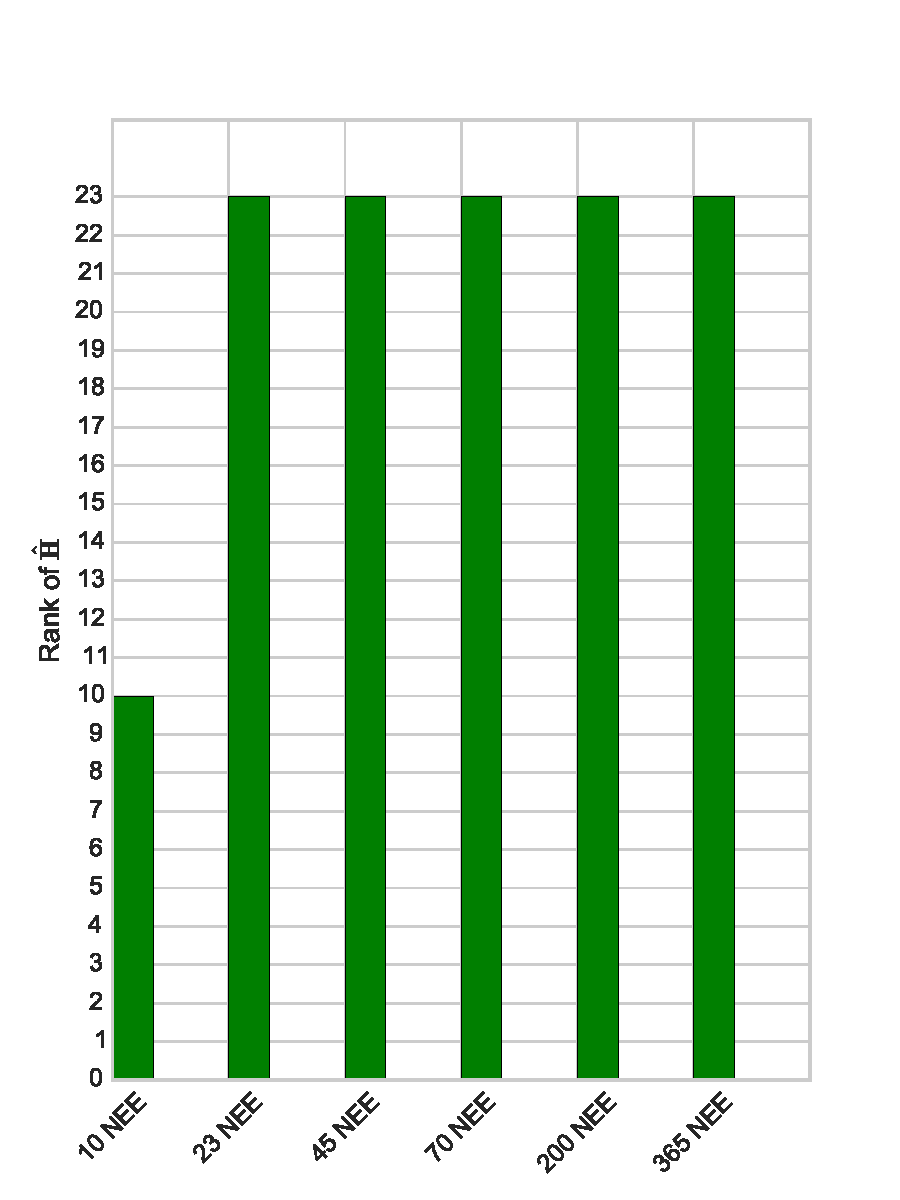
\includegraphics[width=\textwidth]{chapter/chapter5/dalec2_obsrankcvtwind.pdf}
        \caption{Rank of $\hat{\textbf{R}}^{-1/2}\hat{\textbf{H}}\textbf{D}^{1/2}$}
        \label{fig:D2_observailityrankcvtwind}
    \end{subfigure}
    \begin{subfigure}[b]{0.4\textwidth}
        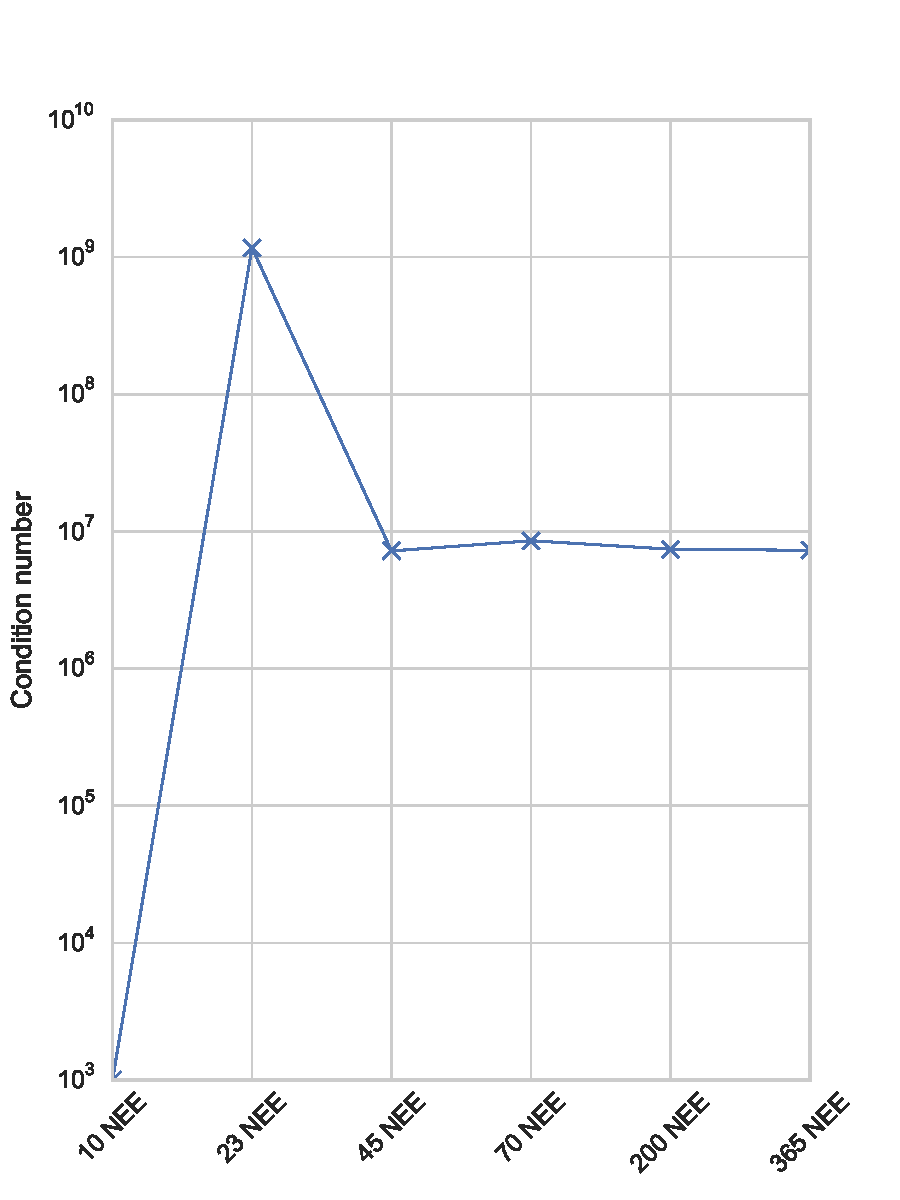
\includegraphics[width=\textwidth]{chapter/chapter5/dalec2_obsrankcondcvtwind.pdf}
        \caption{Condition number of $\hat{\textbf{R}}^{-1/2}\hat{\textbf{H}}\textbf{D}^{1/2}$}
        \label{fig:D2_observabilitycondcvtwind}
    \end{subfigure}
    \caption{Observability of the CVT DALEC2 system for $\hat{\textbf{R}}^{-1/2}\hat{\textbf{H}}\textbf{D}^{1/2}$ with an increasing number of NEE observations randomly distributed through a 1 year assimilation window (left). Condition number for the $\hat{\textbf{R}}^{-1/2}\hat{\textbf{H}}\textbf{D}^{1/2}$ matrices (right).}
    \label{fig:D2_cvtobservabilitywind}
\end{figure}


\subsection{DALEC1 information content} \label{sec:D1_IC} %%%%%%%%%%%%%%%%%%% 
\subsubsection{Information content for a single observation} \label{sec:info_con_single_time}

For the DALEC1 state estimation we can calculate the analytic representation of the information content measures discussed in section~\ref{sec:IC}. This will allow us to understand how the information content changes for differing numbers of observations, different observation types and the effect of including observation error correlations in the assimilation scheme, before moving onto work with the larger DALEC2 joint parameter and state estimation case. For these experiments the elements of the state vector have corresponding background standard deviations $ \sigma_{cfol, b}, \sigma_{croo, b}, \sigma_{cwoo, b}, \sigma_{clit, b}, \sigma_{csom, b}$. We then have
\begin{equation}
\textbf{B} = \begin{pmatrix} 
\sigma_{cfol,b}^{2} & 0 & 0 & 0 & 0 \\
0 & \sigma_{croo,b}^{2} & 0 & 0 & 0 \\
0 & 0 & \sigma_{cwoo,b}^{2} & 0 & 0 \\
0 & 0 & 0 & \sigma_{clit,b}^{2} & 0 \\
0 & 0 & 0 & 0 & \sigma_{csom,b}^{2} \\
\end{pmatrix}. \label{eqn:BmatD1}
\end{equation}   

We begin by considering the Shannon Information Content (SIC) and degrees of freedom for signal (\(dfs\)) for a single observation of LAI. We have the linearised observation operator
\begin{equation}
\textbf{H}_{i} = \frac{\partial LAI^{i}}{\partial \textbf{x}_{i}} = \frac{\partial}{\partial \textbf{x}_{i}} \bigg( \frac{C_{fol}^{i}}{c_{lma}} \bigg) =
\begin{pmatrix}
\frac{1}{c_{lma}} & 0 & 0 & 0 & 0
\end{pmatrix}.
\end{equation}
As we have a single observation at one time, our observation error covariance matrix, $\bf{R}$, is just the variance of our observation of LAI at time $t_0$ ($\sigma_{LAI,o}^{2}$). Therefore,
\begin{equation}
\mathbf{R}_i=\sigma_{LAI,o}^{2}.
\end{equation}
We then have from equation ({\color{red}ref. A matrix eqn}),
\begin{equation}
\begin{array} {lcl}
\mathbf{A} &=& (\mathbf{J}'')^{-1} \\
&=& (\mathbf{B}^{-1}+\hat{\mathbf{H}}^{T}\hat{\mathbf{R}}^{-1}\hat{\mathbf{H}})^{-1} \\
&=& (\mathbf{B}^{-1}+\mathbf{H}_0^{T}\mathbf{R}_0^{-1}\mathbf{H}_0)^{-1} \\
&=& \begin{pmatrix} 
\frac{c_{lma}^2 \sigma_{LAI,o}^2 \sigma_{cfol,b}^2}{\sigma_{cfol,b}^2 + c_{lma}^2 \sigma_{LAI,o}^2} & 0 & 0 & 0 & 0 \\
0 & \sigma_{croo,b}^{2} & 0 & 0 & 0 \\
0 & 0 & \sigma_{cwoo,b}^{2} & 0 & 0 \\
0 & 0 & 0 & \sigma_{clit,b}^{2} & 0 \\
0 & 0 & 0 & 0 & \sigma_{csom,b}^{2} \\
\end{pmatrix}.
\end{array}
\end{equation} 
We can now derive the SIC and $dfs$ using equation \eqref{eqn:sic} and \eqref{eqn:dfs} as,
\begin{equation}
\text{SIC} = \frac{1}{2}\text{ln}\frac{\begin{vmatrix} \mathbf{B} \end{vmatrix}}{\begin{vmatrix} \mathbf{A} \end{vmatrix}} = \frac{1}{2}\text{ln}\frac{(c_{lma}^2 \sigma_{LAI,o}^{2}+\sigma_{cfol,b}^{2})}{c_{lma}^2 \sigma_{LAI,o}^{2}}
=\frac{1}{2}\text{ln} \bigg(1+\frac{\sigma_{cfol,b}^{2}}{c_{lma}^2 \sigma_{LAI,o}^{2}}\bigg) \label{eqn:siclai}
\end{equation}
and 
\begin{equation}
dfs = n - tr(\textbf{B}^{-1}\textbf{A}) = 5 - \bigg(\frac{c_{lma}^2 \sigma_{LAI,o}^{2}}{(c_{lma}^2 \sigma_{LAI,o}^{2}+\sigma_{cfol,b}^{2})} + 4 \bigg) = 1 -\frac{c_{lma}^2 \sigma_{LAI,o}^{2}}{(c_{lma}^2 \sigma_{LAI,o}^{2}+\sigma_{cfol,b}^{2})}. \label{eqn:dfslai}
\end{equation}
We see that in general for a direct observation of any of the carbon pools $C$ we have
\begin{equation}
\text{SIC} =\frac{1}{2}\text{ln} \bigg(1+\frac{\sigma_{c,b}^{2}}{\sigma_{c,o}^{2}}\bigg) \label{eqn:sicC}
\end{equation}
and 
\begin{equation}
dfs = 1 -\frac{\sigma_{c,o}^{2}}{(\sigma_{c,o}^{2}+\sigma_{c,b}^{2})}, \label{eqn:dfsC}
\end{equation}
where $\sigma_{c,o}$ and $\sigma_{c,b}$ are the observation and background standard deviations respectively, corresponding to any of the 5 carbon pools.
We see the SIC for a single observation of one of the carbon pools is dependent on the ratio between the observation and background variances. The carbon pool observation which will give us the highest SIC is the observation with the largest ratio $\frac{\sigma_{c,b}^{2}}{\sigma_{c,o}^{2}}$. This is also the case for $dfs$. Assuming a fixed background standard deviation, the carbon pool observation which will give us the highest information content is the pool which we can measure most accurately, as expected. From equations~\eqref{eqn:siclai} and \eqref{eqn:dfslai} for an observation of LAI the information content is also dependent on $c_{lma}$ the parameter describing leaf mass area.

Next we consider the information content in a single observation of NEE. We have
\begin{equation}
\textbf{H}_{i} = \frac{\partial NEE^{i}}{\partial \textbf{x}_{i}} =
\begin{pmatrix}
-(1-f_{auto})\zeta^i & 0 & 0 & \theta_{lit} e^{\Theta T^{i}} & \theta_{som} e^{\Theta T^{i}}
\end{pmatrix}
\end{equation}
and
\begin{equation}
\mathbf{R}_i = \sigma_{NEE,o}^{2}.
\end{equation}
We then find
\begin{equation}
\text{SIC} = \frac{1}{2}\text{ln}\Bigg(1 + \frac{(f_{auto}-1)^{2}(\zeta^{i})^{2}\sigma_{cfol,b}^{2} + (e^{\Theta T^{i}})^2(\theta_{som}^2\sigma_{csom,b}^2+\theta_{lit}^2\sigma_{clit,b}^2)}{\sigma_{NEE,o}^{2}}\Bigg) \label{eqn:sicnee}
\end{equation}
and
\begin{equation}
dfs = 1 - \frac{\sigma_{NEE,o}^{2}}{(f_{auto}-1)^{2}(\zeta^{i})^{2}\sigma_{cfol,b}^{2}+(e^{\Theta T^{i}})^2(\theta_{som}^2\sigma_{csom,b}^2+\theta_{lit}^2\sigma_{clit,b}^2) +\sigma_{NEE,o}^{2}}. \label{eqn:dfsnee}
\end{equation}
We see that Equations~\eqref{eqn:sicnee} and \eqref{eqn:dfsnee} have a similar form to Equations~\eqref{eqn:sicC} and \eqref{eqn:dfsC}. The information content is again dependent on the ratio between the observation and background variances. The information content for the observations of NEE is also dependent on the magnitude of the first derivative of GPP with respect to \(C_{fol}\) and the magnitude of the exponential function of temperature controlling the rate of heterotrophic respiration, \(e^{\Theta T^{i}}\). Both the first derivative of GPP and  \(e^{\Theta T^{i}}\) will be of greater magnitude when we have higher mean daily temperatures. This means that observations of NEE made at times with higher temperatures will have higher information content and more of an impact on data assimilation results.
\begin{figure}[ht]
    \centering
    \begin{subfigure}[b]{0.45\textwidth}
        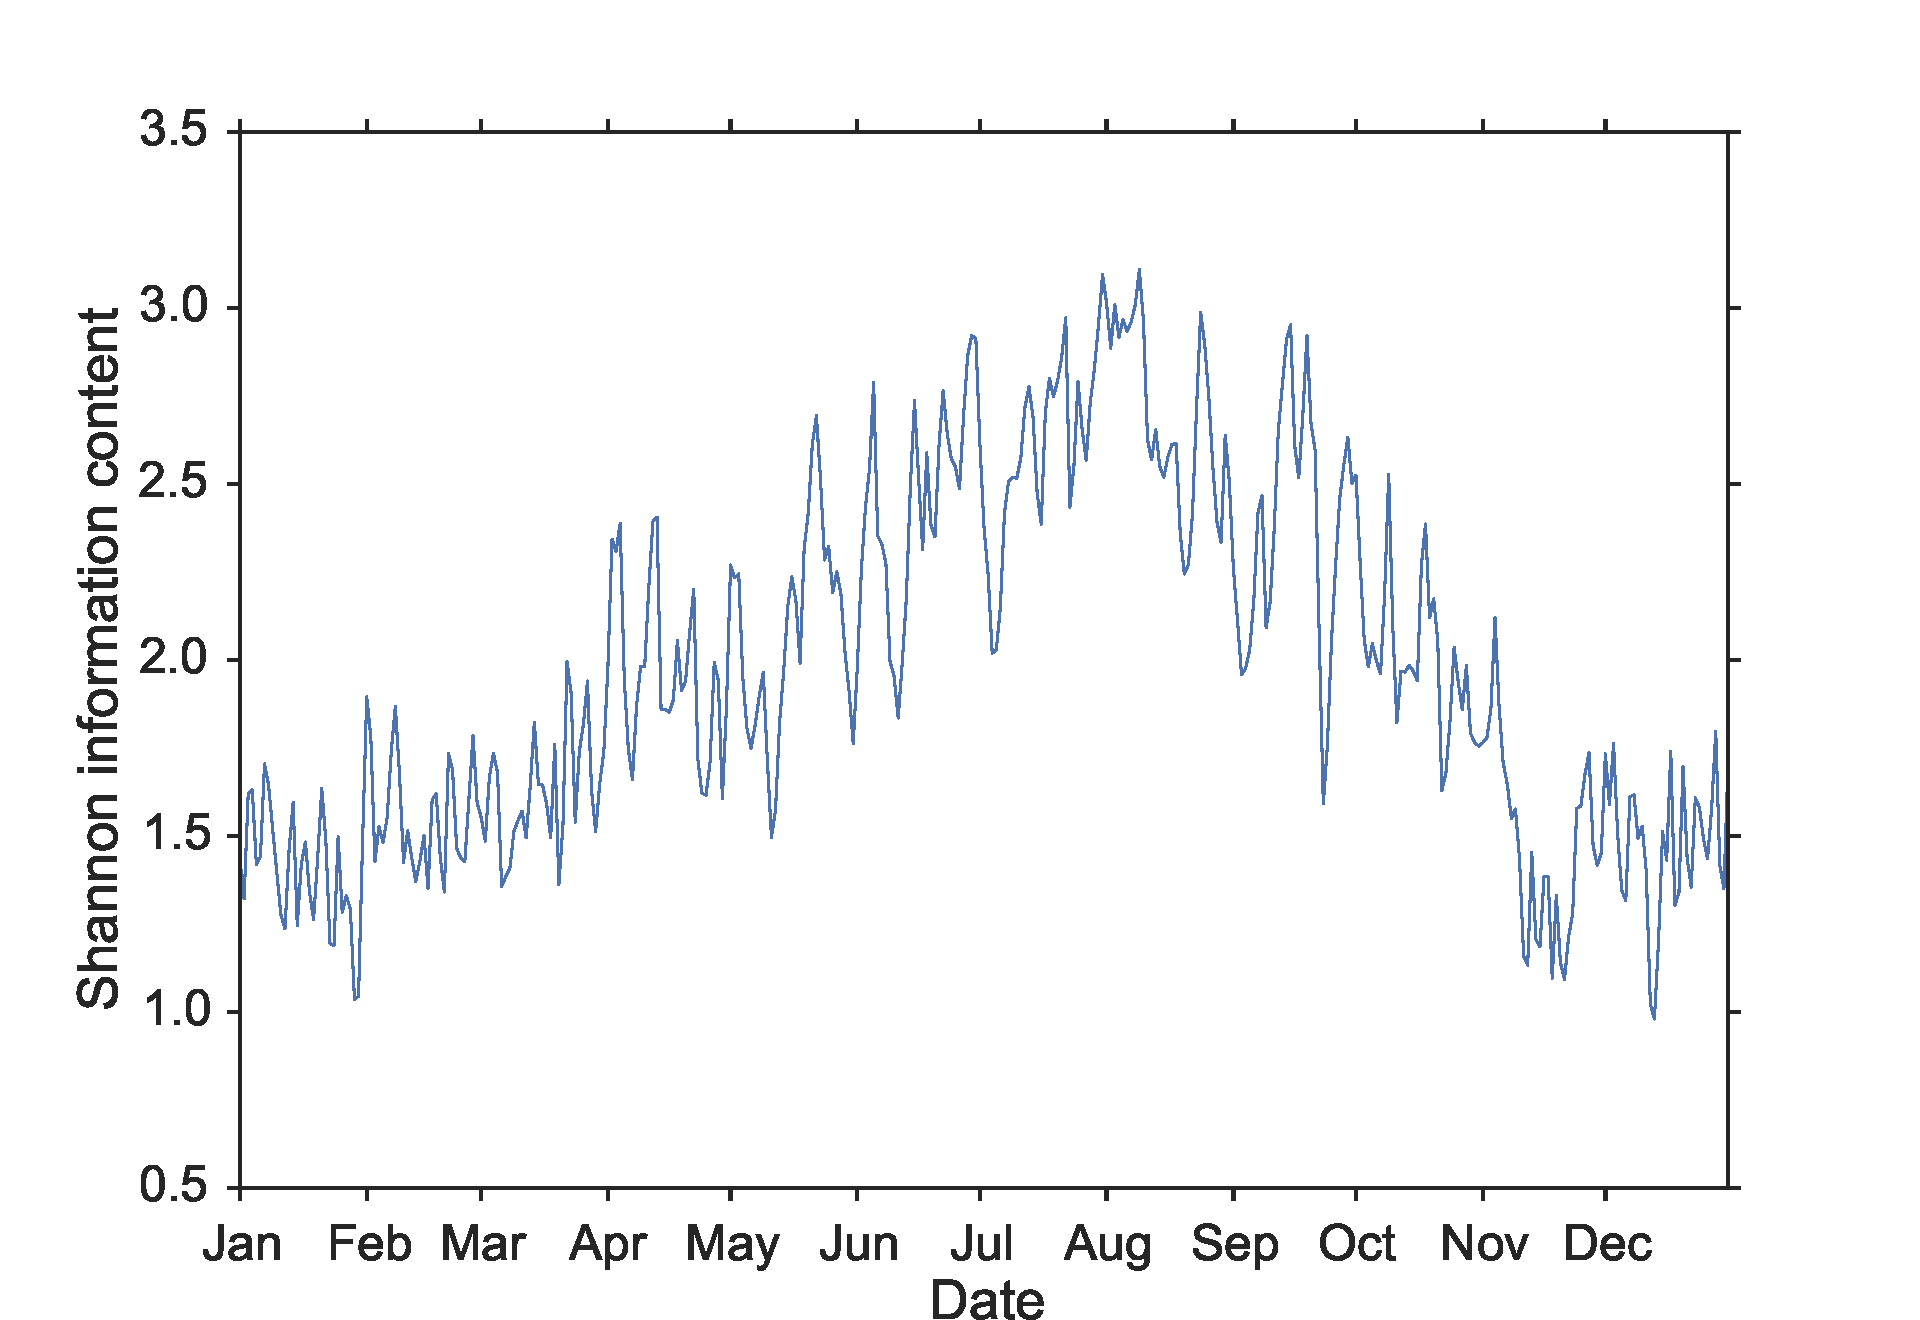
\includegraphics[width=\textwidth]{chapter/chapter5/oregon2007SICnee.pdf}
        \caption{SIC for single NEE observation}
        \label{fig:sic_nee_oregon2007}
    \end{subfigure}%
    \begin{subfigure}[b]{0.45\textwidth}
        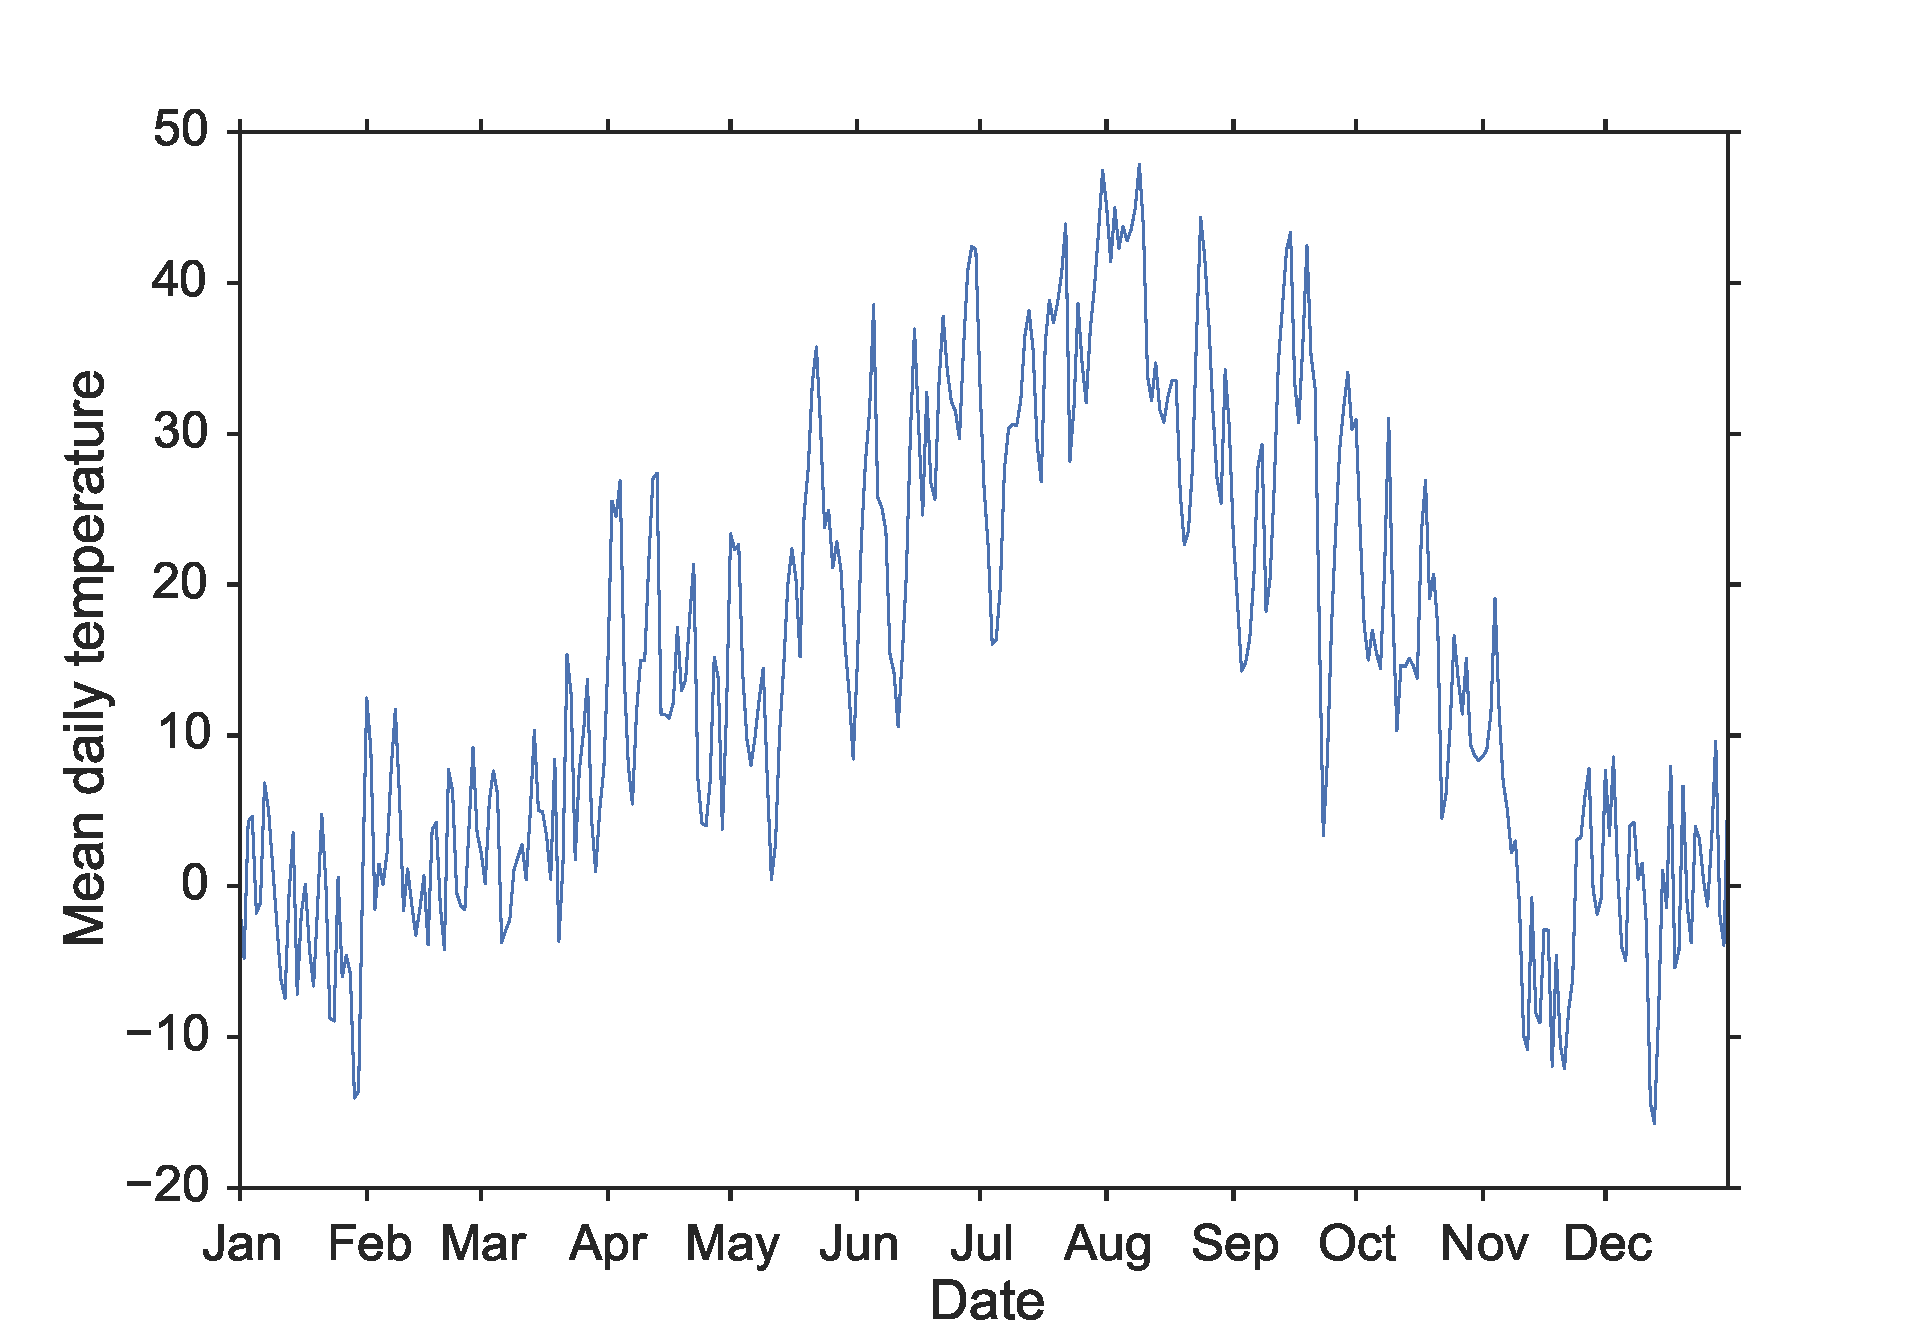
\includegraphics[width=\textwidth]{chapter/chapter5/oregon2007temp.pdf}
        \caption{Mean daily temperature for year's data}
        \label{fig:temp_nee_oregon2007}
    \end{subfigure}
    \caption{SIC for a single NEE observation changing throughout a year's window using driving data from a forest of ponderosa pine in Oregon taken in 2007 (left). Mean daily temperature for the same site and period (right).}
    \label{fig:neeSIC_temp_comp}
\end{figure}

In Figure~\ref{fig:neeSIC_temp_comp} we show how closely SIC is related to mean daily temperature for NEE observations throughout a year's window using daily driving data from a forest of ponderosa pine in Oregon (as described in section~\ref{sec:oregon}). Higher information content in summer observations of NEE makes physical sense. In summertime fluxes of carbon through the forest ecosystem are of greater magnitude than in winter, with more photosynthesis and respiration occurring. This gives us more information about the fluxes of carbon through our system in summertime observations of NEE. It is important to consider this result when planning for down time or routine maintenance at flux tower sites measuring NEE. The temperature dependence of information content will also hold true for other observations whose observation operators include the nonlinear temperature term controlling heterotrophic respiration. These observations include ground respiration, measured using soil respiration chambers, and total ecosystem respiration, estimated from nighttime NEE measurements.

In Figure~\ref{fig:sic_nee_oregon2007} we have assumed constant prior and observation standard deviations. This is an accurate assumption for our prior errors. However, it has been shown that NEE errors are heteroscedastic \citep{Richardson200838} and therefore scale with the magnitude of the flux. This would reduce the magnitude of the results shown in Figure~\ref{fig:sic_nee_oregon2007}, as our standard deviation in observations of summer NEE would be larger, reducing the information content.

For Figure~\ref{fig:sic_nee_oregon2007} we have used a numerical implementation in Python to calculate the SIC varying for 365 days of driving data. It is important to test our numerical implementation for correctness. In table~\ref{table:correctness_test} we show the SIC and \(dfs\) calculated both analytically and numerically. From this table we can see that both analytic and numerical implementations give us the same result to 15 or more significant figures. This gives us a degree of confidence that our implementation is also correct for DALEC2. In this table we have assumed constant prior and observation standard deviations for the carbon pools.

\begin{table}[ht] 
%\begin{center}
\centering
	\begin{tabular}{| l | l | l | l | l |}
	\hline
	Obs. & SIC analytic value & SIC numeric value & \(dfs\) analytic value & \(dfs\) numeric value \\ \hline
	NEE & 0.0209343224569909 & 0.0209343224569913 & 0.0410042587324008 & 0.0410042587324008 \\ \hline
	\(C_{fol}\) & 0.8047189562170501 & 0.8047189562170515 & 0.7999999999999998 & 0.7999999999999998 \\ \hline
	\(C_{roo}\) & 0.1838623900626585 & 0.1838623900626572 & 0.3076923076923075 & 0.3076923076923083 \\ \hline 	
	\(C_{woo}\)& 0.8047189562170501 & 0.8047189562170515 & 0.7999999999999998 & 0.7999999999999998 \\ \hline
	\(C_{lit}\) & 0.1838623900626585 & 0.1838623900626572 & 0.3076923076923075 & 0.3076923076923074 \\ \hline
	\(C_{som}\) & 0.1838623900626585 & 0.1838623900626572 & 0.3076923076923075 & 0.3076923076923074 \\
	\hline
	\end{tabular}
	\caption{Correctness tests showing numeric and analytic values of information content calculated using 2007 driving data and parameter values from an Oregon ponderosa pine forest.}
	\label{table:correctness_test}
%\end{center} 
\end{table}

\subsubsection{Information content for observations at a single time}

We next consider the SIC when we have more than one observation at a single time. Here we will investigate the representation of information content when assimilating an observation of NEE with an observation of a carbon pool state member. We begin with a single observation of NEE and an observation of \(C_{fol}\). We have the linearised observation operator,
\begin{equation}
\textbf{H}_{i} = \frac{\partial}{\partial \textbf{x}_{i}}\big(NEE^{i}, C_{fol}^{i} \big) =
 \begin{pmatrix}
-(1-f_{auto})\zeta^i & 0 & 0 & \theta_{lit} e^{\Theta T^{i}} & \theta_{som} e^{\Theta T^{i}}\\
1 & 0 & 0 & 0 & 0
\end{pmatrix}
\end{equation}
and observation error covariance matrix
\begin{equation}
\mathbf{R}_i = \begin{pmatrix}
\sigma_{NEE,o}^{2} & 0 \\
0 & \sigma_{cfol,o}^{2}
\end{pmatrix}.
\end{equation}
We then find,
\begin{equation}
\text{SIC} = \frac{1}{2}\text{ln} \Bigg( 1 + \frac{\sigma_{cfol,b}^{2}}{\sigma_{cfol,o}^{2}} + \frac{\xi^{i}}{\sigma_{NEE,o}^{2}} + \\
 \frac{\sigma_{cfol,b}^{2}(e^{\Theta T^{i}})^2(\theta_{som}^2\sigma_{csom,b}^2+\theta_{lit}^2\sigma_{clit,b}^2)}{\sigma_{NEE,o}^{2}\sigma_{cfol,o}^{2}} \Bigg) \label{eqn:sicneecfol}
 \end{equation}
 where, \( \xi^{i} = (f_{auto}-1)^{2}(\zeta^{i})^{2}\sigma_{cfol,b}^{2} + (e^{\Theta T^{i}})^2(\theta_{som}^2\sigma_{csom,b}^2+\theta_{lit}^2\sigma_{clit,b}^2) \). From equation~\eqref{eqn:sicneecfol} we can see that we have the first order terms for both NEE and \(C_{fol}\) as in equations~\eqref{eqn:sicC} and \eqref{eqn:sicnee}. We also have a second order term for the combination of these observations. We can repeat this for the other carbon pools and find for \(\textbf{H}_{i} = \frac{\partial}{\partial \textbf{x}_{i}}\big(NEE^{i}, C_{roo}^{i} \big) \),
\begin{equation}
\text{SIC} = \frac{1}{2}\text{ln} \Bigg( 1 + \frac{\sigma_{croo,b}^{2}}{\sigma_{croo,o}^{2}} + \frac{\xi^{i}}{\sigma_{NEE,o}^{2}} + \\
 \frac{\sigma_{croo,b}^{2}\big((f_{auto}-1)^{2}(\zeta^{i})^{2}\sigma_{cfol,b}^{2} + (e^{\Theta T^{i}})^2(\theta_{som}^2\sigma_{csom,b}^2+\theta_{lit}^2\sigma_{clit,b}^2)\big)}{\sigma_{NEE,o}^{2}\sigma_{croo,o}^{2}} \Bigg), \label{eqn:sicneecroo}
 \end{equation} 
for \(\textbf{H}_{i} = \frac{\partial}{\partial \textbf{x}_{i}}\big(NEE^{i}, C_{woo}^{i} \big) \),
\begin{equation}
\text{SIC} = \frac{1}{2}\text{ln} \Bigg( 1 + \frac{\sigma_{cwoo,b}^{2}}{\sigma_{cwoo,o}^{2}} + \frac{\xi^{i}}{\sigma_{NEE,o}^{2}} + \\
 \frac{\sigma_{cwoo,b}^{2}\big((f_{auto}-1)^{2}(\zeta^{i})^{2}\sigma_{cfol,b}^{2} + (e^{\Theta T^{i}})^2(\theta_{som}^2\sigma_{csom,b}^2+\theta_{lit}^2\sigma_{clit,b}^2)\big)}{\sigma_{NEE,o}^{2}\sigma_{cwoo,o}^{2}} \Bigg), \label{eqn:sicneecwoo}
 \end{equation}
 for \(\textbf{H}_{i} = \frac{\partial}{\partial \textbf{x}_{i}}\big(NEE^{i}, C_{lit}^{i} \big) \),
 \begin{equation}
\text{SIC} = \frac{1}{2}\text{ln} \Bigg( 1 + \frac{\sigma_{clit,b}^{2}}{\sigma_{clit,o}^{2}} + \frac{\xi^{i}}{\sigma_{NEE,o}^{2}} + \\
 \frac{\sigma_{clit,b}^{2}\big((f_{auto}-1)^{2}(\zeta^{i})^{2}\sigma_{cfol,b}^{2} + (e^{\Theta T^{i}})^2\theta_{som}^2\sigma_{csom,b}^2\big)}{\sigma_{NEE,o}^{2}\sigma_{clit,o}^{2}} \Bigg) \label{eqn:sicneeclit}
 \end{equation}
 and for \(\textbf{H}_{i} = \frac{\partial}{\partial \textbf{x}_{i}}\big(NEE^{i}, C_{som}^{i} \big) \),
 \begin{equation}
\text{SIC} = \frac{1}{2}\text{ln} \Bigg( 1 + \frac{\sigma_{csom,b}^{2}}{\sigma_{csom,o}^{2}} + \frac{\xi^{i}}{\sigma_{NEE,o}^{2}} + \\
 \frac{\sigma_{csom,b}^{2}\big((f_{auto}-1)^{2}(\zeta^{i})^{2}\sigma_{cfol,b}^{2} + (e^{\Theta T^{i}})^2\theta_{lit}^2\sigma_{clit,b}^2\big)}{\sigma_{NEE,o}^{2}\sigma_{csom,o}^{2}} \Bigg). \label{eqn:sicneecsom}
 \end{equation}
Assuming constant prior and observation standard deviations across our carbon pool observations we see that the information content will be largest in equations~\eqref{eqn:sicneecroo} and \eqref{eqn:sicneecwoo}. For both \(\textbf{H}_{i} = \frac{\partial}{\partial \textbf{x}_{i}}\big(NEE^{i}, C_{roo}^{i} \big) \) and \(\textbf{H}_{i} = \frac{\partial}{\partial \textbf{x}_{i}}\big(NEE^{i}, C_{woo}^{i} \big) \) we have an extra term in the numerator for our second order term corresponding to the combination of the two observations. If we consider the linearised observation operator for both these cases,
\begin{equation}
\textbf{H}_{i} = \frac{\partial}{\partial \textbf{x}_{i}}\big(NEE^{i}, C_{roo}^{i} \big) =
 \begin{pmatrix}
-(1-f_{auto})\zeta^i & 0 & 0 & \theta_{lit} e^{\Theta T^{i}} & \theta_{som} e^{\Theta T^{i}}\\
0 & 1 & 0 & 0 & 0
\end{pmatrix}
\end{equation}
and
\begin{equation}
\textbf{H}_{i} = \frac{\partial}{\partial \textbf{x}_{i}}\big(NEE^{i}, C_{woo}^{i} \big) =
 \begin{pmatrix}
-(1-f_{auto})\zeta^i & 0 & 0 & \theta_{lit} e^{\Theta T^{i}} & \theta_{som} e^{\Theta T^{i}}\\
0 & 0 & 1 & 0 & 0
\end{pmatrix},
\end{equation}
we can see that these observations provide an orthogonal constraint to the observation of NEE. Neither of these pools are observed with a single observation of NEE. The information content being greater when assimilating \(C_{roo}\) or \(C_{woo}\) alongside NEE is therefore expected. 

In practice we cannot assume constant prior and observation errors across the different carbon pools. Root carbon is hard to measure accurately \citep{brown2002measuring}. However, woody biomass (\(C_{woo}\)) is regularly measured using mensuration \citep{husch2002forest} or point-centred quarter methods \citep{dahdouh2006empirical} at forest sites. Advancements in Light Detection And Ranging (LiDAR) scanning \citep{Lefsky199983} mean that we have increasingly more accurate observations of woody biomass. The European Space Agency BIOMASS mission \citep{le2011biomass} will also provide a much more abundant source of woody biomass measurements in the future. If we consider NEE to be the main observation currently used in ecosystem data assimilation, then the increasing number of available woody biomass measurements will benefit assimilation schemes greatly.

\subsubsection{Information content in successive observations} \label{sec:D1_succ_obs}

In section~\ref{sec:info_con_single_time} we investigate the information in observation for DALEC1 at a single time. In this section we will consider successive observations in time. It has been shown that the SIC in observations is additive with successive observations in time. The proof for this can be found in appendix A.1 of \citet{Fowler2012}. We can see this if we calculate the SIC for successive observations of foliar carbon, \(C_{fol}\). We have the linearised observation operator and observation error covariance matrix at time $t_i$,
\begin{equation}
\mathbf{H}_{i} = \frac{\partial C_{fol}^{i}}{\partial \textbf{x}_i} = \begin{pmatrix}
1 & 0 & 0 & 0 & 0
\end{pmatrix}
\hspace{5mm} \text{and} \hspace{5mm}
\mathbf{R}_i=\sigma_{cfol,o}^{2}.
\end{equation}
For two successive observations of \(C_{fol}\) we have,
\begin{equation}
\hat{\mathbf{H}}=
\begin{pmatrix}
\mathbf{H}_0 \\
\mathbf{H}_1\mathbf{M}_0\\
\end{pmatrix}
=
\begin{pmatrix}
1 & 0 & 0 & 0 & 0 \\
(1-\theta_{fol})+f_{fol}(1-f_{auto})\zeta^0 & 0 & 0 & 0 & 0\\
\end{pmatrix}
\end{equation}
and
\begin{equation}
\hat{\mathbf{R}}=
\begin{pmatrix}
\mathbf{R}_0 & 0  \\
0 & \mathbf{R}_1  \\
\end{pmatrix}
=
\begin{pmatrix}
\sigma_{cfol,o}^{2} & 0  \\
0 & \sigma_{cfol,o}^{2}  \\
\end{pmatrix}.
\end{equation}
We then have,
\begin{equation}
SIC = \frac{1}{2}\text{ln}\frac{\begin{vmatrix} \mathbf{B} \end{vmatrix}}{\begin{vmatrix} \mathbf{A} \end{vmatrix}} =\frac{1}{2}\text{ln} \bigg(1+\frac{\sigma_{cfol,b}^{2}}{\sigma_{cfol,o}^{2}}+\frac{\sigma_{cfol,b}^{2}\eta_0^{2}}{\sigma_{cfol,o}^{2}} \bigg), \label{eq:sic_2cfol}
\end{equation}
where $\eta_i=(1-\theta_{fol})+f_{fol}(1-f_{auto})\zeta^{i}$. We see this is similar to equation~\eqref{eqn:sicC} for the SIC of a single carbon pool observation but with an added term evolved by the linearised model. Here the second term is multiplied by \(\eta_{0}^2\) which is the square of the first element of the linearised model \(\mathbf{M}_0\). We can continue adding more observations at successive times. For three observations at successive times we have,
\begin{equation}
SIC =\frac{1}{2}\text{ln} \bigg(1+\frac{\sigma_{cfol,b}^{2}}{\sigma_{cfol,o}^{2}}+\frac{\sigma_{cfol,b}^{2}\eta_0^{2}}{\sigma_{cfol,o}^{2}}+\frac{\sigma_{cfol,b}^{2}\eta_0^{2}\eta_1^{2}}{\sigma_{cfol,o}^{2}} \bigg),
\end{equation}
for four,
\begin{equation}
SIC =\frac{1}{2}\text{ln} \bigg(1+\frac{\sigma_{cfol,b}^{2}}{\sigma_{cfol,o}^{2}}+\frac{\sigma_{cfol,b}^{2}\eta_0^{2}}{\sigma_{cfol,o}^{2}}+\frac{\sigma_{cfol,b}^{2}\eta_0^{2}\eta_1^{2}}{\sigma_{cfol,o}^{2}}+\frac{\sigma_{cfol,b}^{2}\eta_0^{2}\eta_1^{2}\eta_2^{2}}{\sigma_{cfol,o}^{2}} \bigg).
\end{equation}
Using a simple proof by induction we find that for \(n\) successive observations we have,
\begin{equation}
SIC\text{ for }n\text{ successive observations of }C_{fol} = \frac{1}{2}\text{ln}\bigg(1+\frac{\sigma_{cfol,b}^{2}}{\sigma_{cfol,o}^{2}}\big(1+\sum_{k=0}^{n-2}\prod_{i=0}^{k}\eta_i^{2}\big)\bigg)
\end{equation}
This demonstrates that SIC is additive for successive observations in time. In Figure~\ref{fig:ic_succ_cf} we have plotted the SIC and \(dfs\) for increasing numbers of observations of \(C_{fol}\), using a year of meteorological driving data from a pine stand in Oregon. We see that as successive observations are added the information content tends to a limit where we are adding no new information with extra observations of \(C_{fol}\). For \(dfs\) this limit is one as we are only observing a single degree of freedom so cannot constrain more than a single element of the state. For SIC we add a decreasing amount of information as observations are made further away from the initial state. We find similar results for all other carbon pools. This suggests making observations of any individual carbon pool for a forest site too often is not cost effective as after just a few observations the information you are adding to your system begins to decrease. 

\begin{figure}[ht]
    \centering
    \begin{subfigure}[b]{0.45\textwidth}
        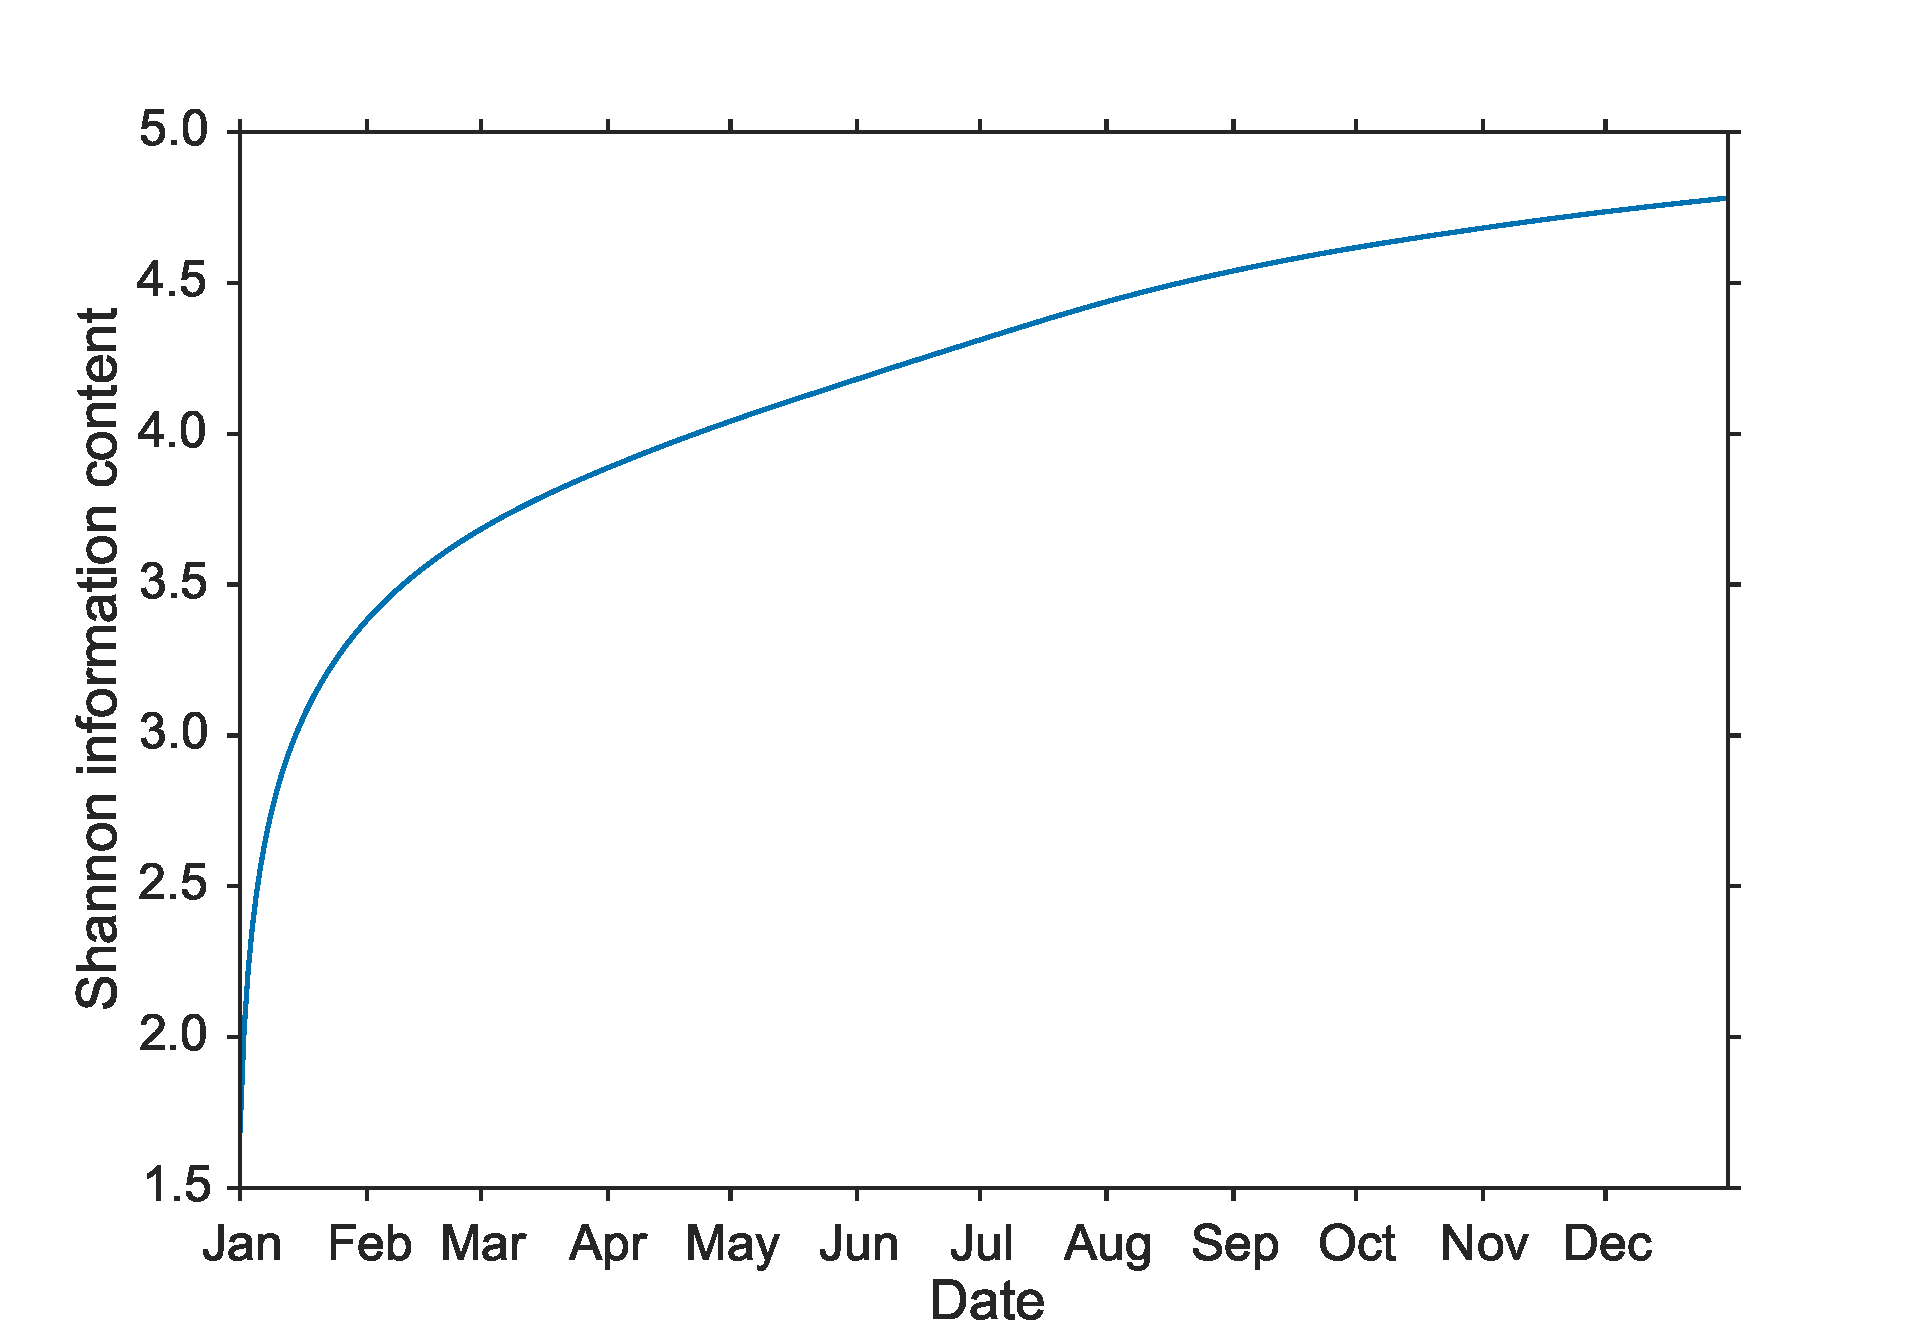
\includegraphics[width=\textwidth]{chapter/chapter5/sic_succ_cf.pdf}
        \caption{SIC for successive \(C_{fol}\) observations}
        \label{fig:sic_succ_cf}
    \end{subfigure}%
    \begin{subfigure}[b]{0.45\textwidth}
        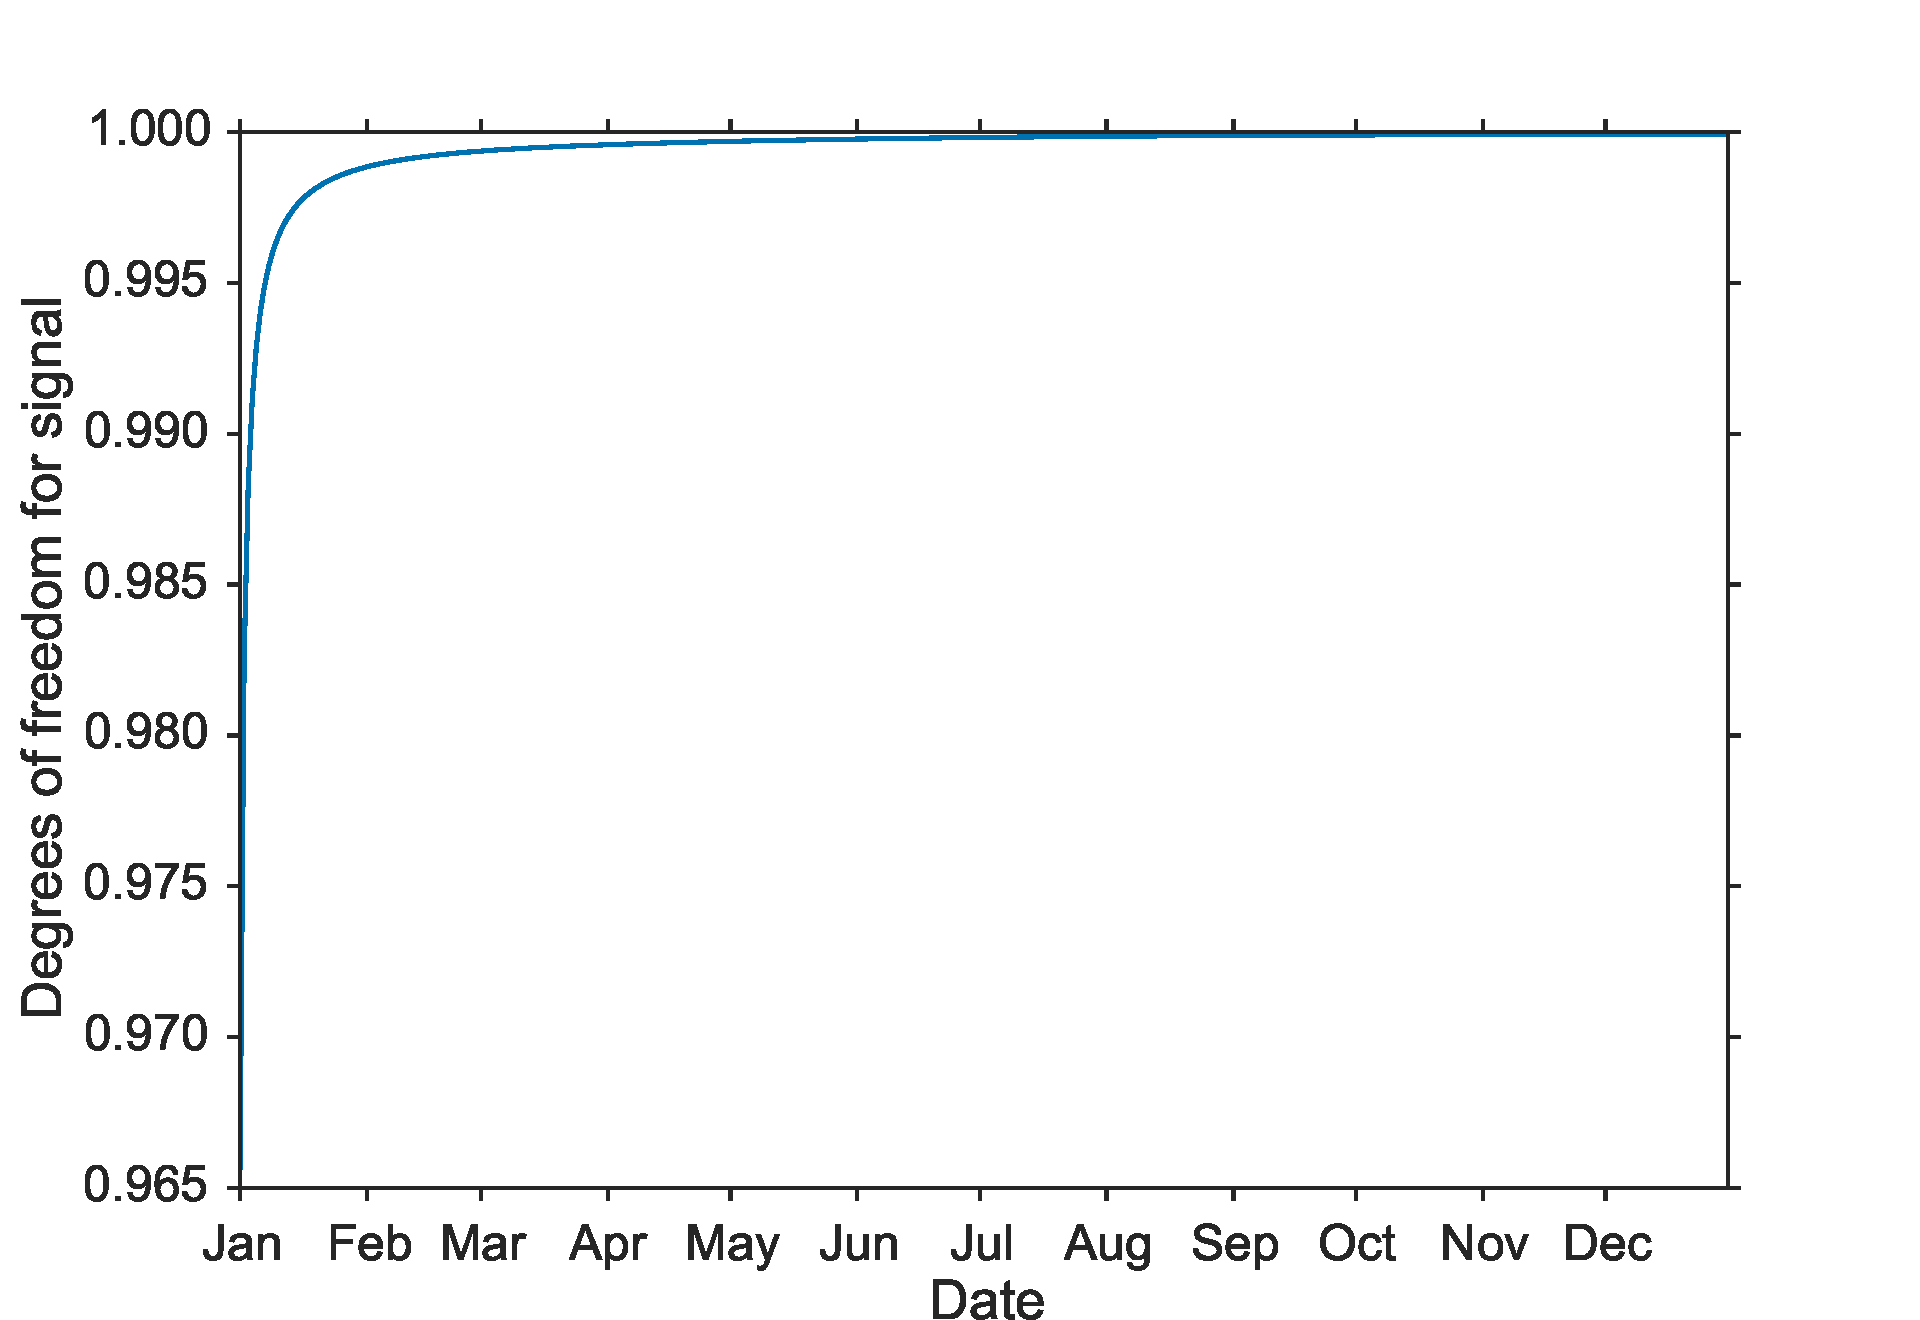
\includegraphics[width=\textwidth]{chapter/chapter5/dfs_succ_cf.pdf}
        \caption{\(dfs\) for successive \(C_{fol}\) observations}
        \label{fig:dfs_succ_cf}
    \end{subfigure}
    \caption{SIC and \(dfs\) for as successive \(C_{fol}\) observations are added throughout a year's window using driving data from a pine stand in Oregon taken in 2007.}
    \label{fig:ic_succ_cf}
\end{figure}

In section~\ref{sec:info_con_single_time} it was shown that observations of NEE made during the summer had significantly higher information content than those made during winter for an evergreen forest site. In figure~\ref{fig:ic_succ_nee} we show that 27 days of successive winter NEE observations (made from January \(1^{\text{st}}\) 2007) are required to give the same information content as a single summer observation of NEE (taken on \( 22^{\text{nd}} \) June 2007).

\begin{figure}[ht]
    \centering
    \begin{subfigure}[b]{0.45\textwidth}
        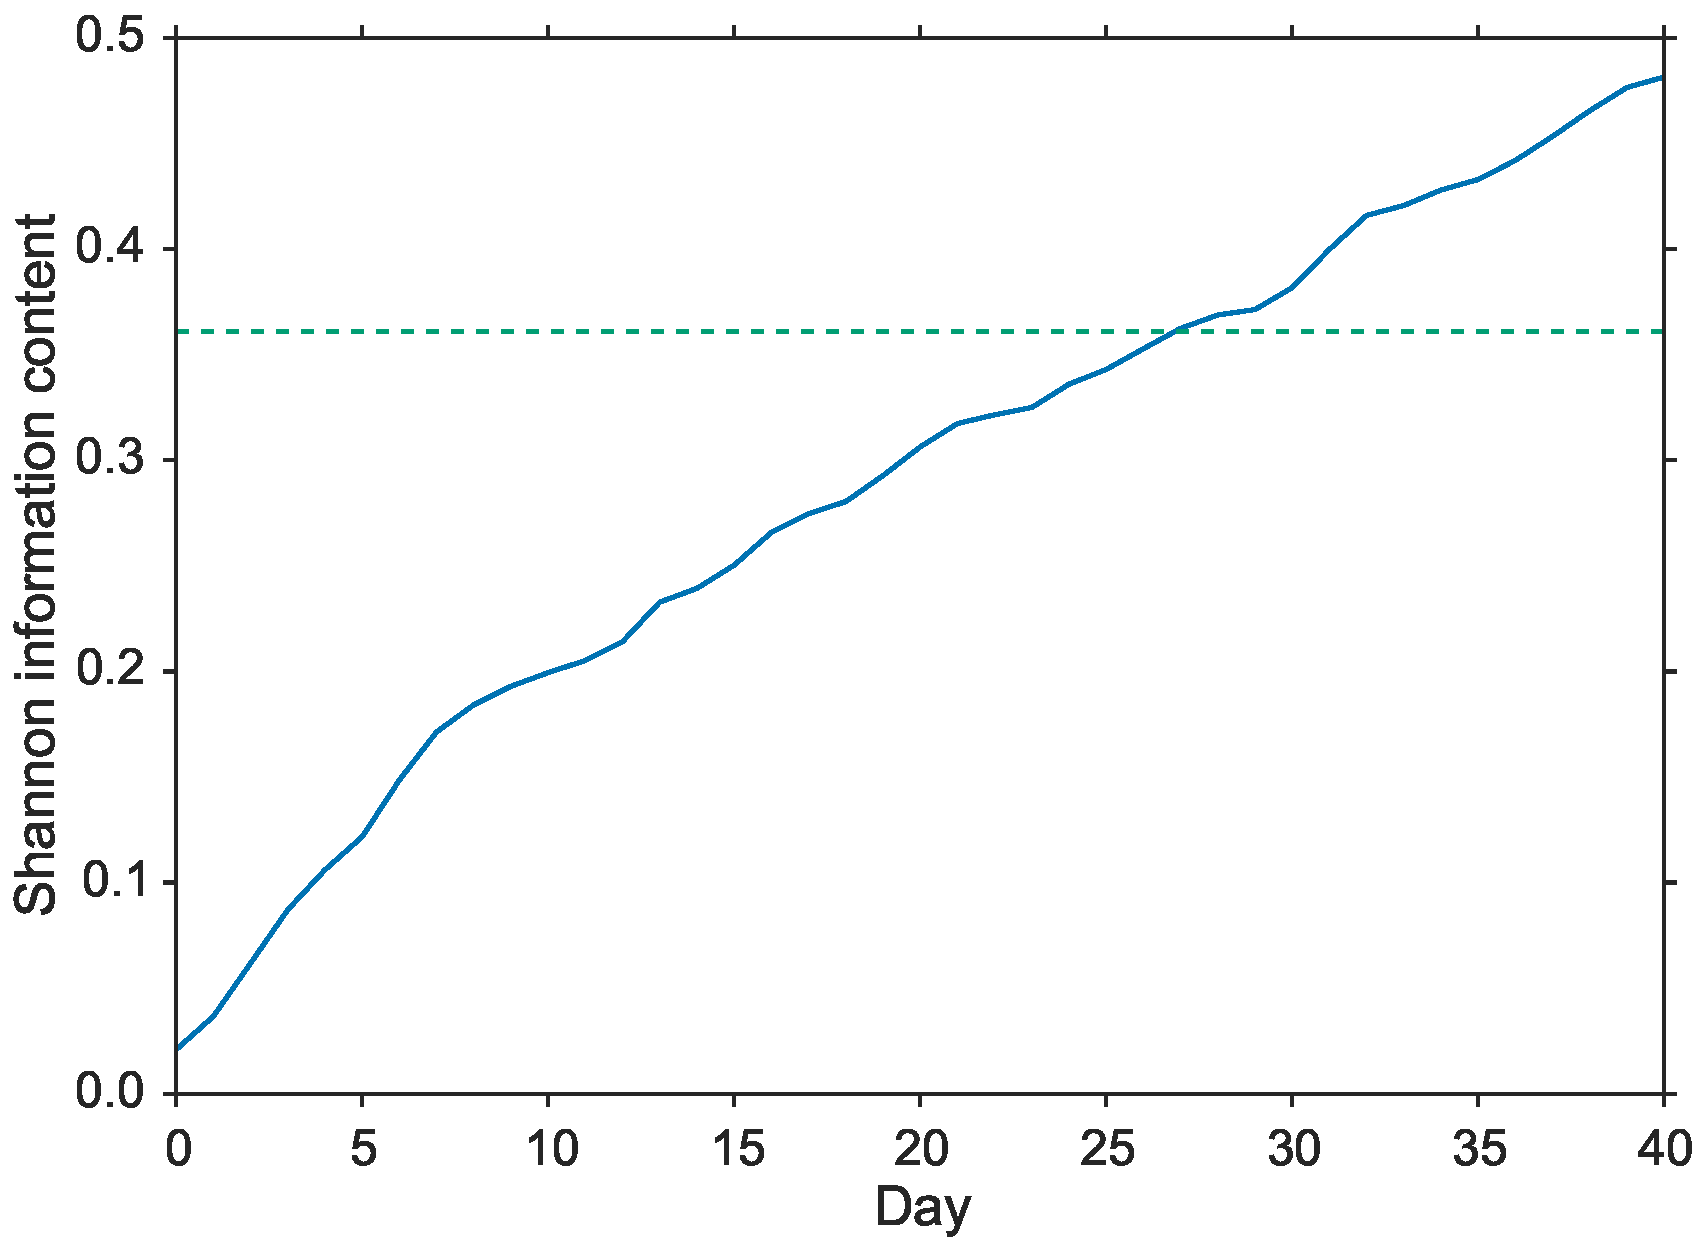
\includegraphics[width=\textwidth]{chapter/chapter5/sic_succ_nee.pdf}
        \caption{SIC for successive NEE observations}
        \label{fig:sic_succ_nee}
    \end{subfigure} \hspace{5mm}
    \begin{subfigure}[b]{0.45\textwidth}
        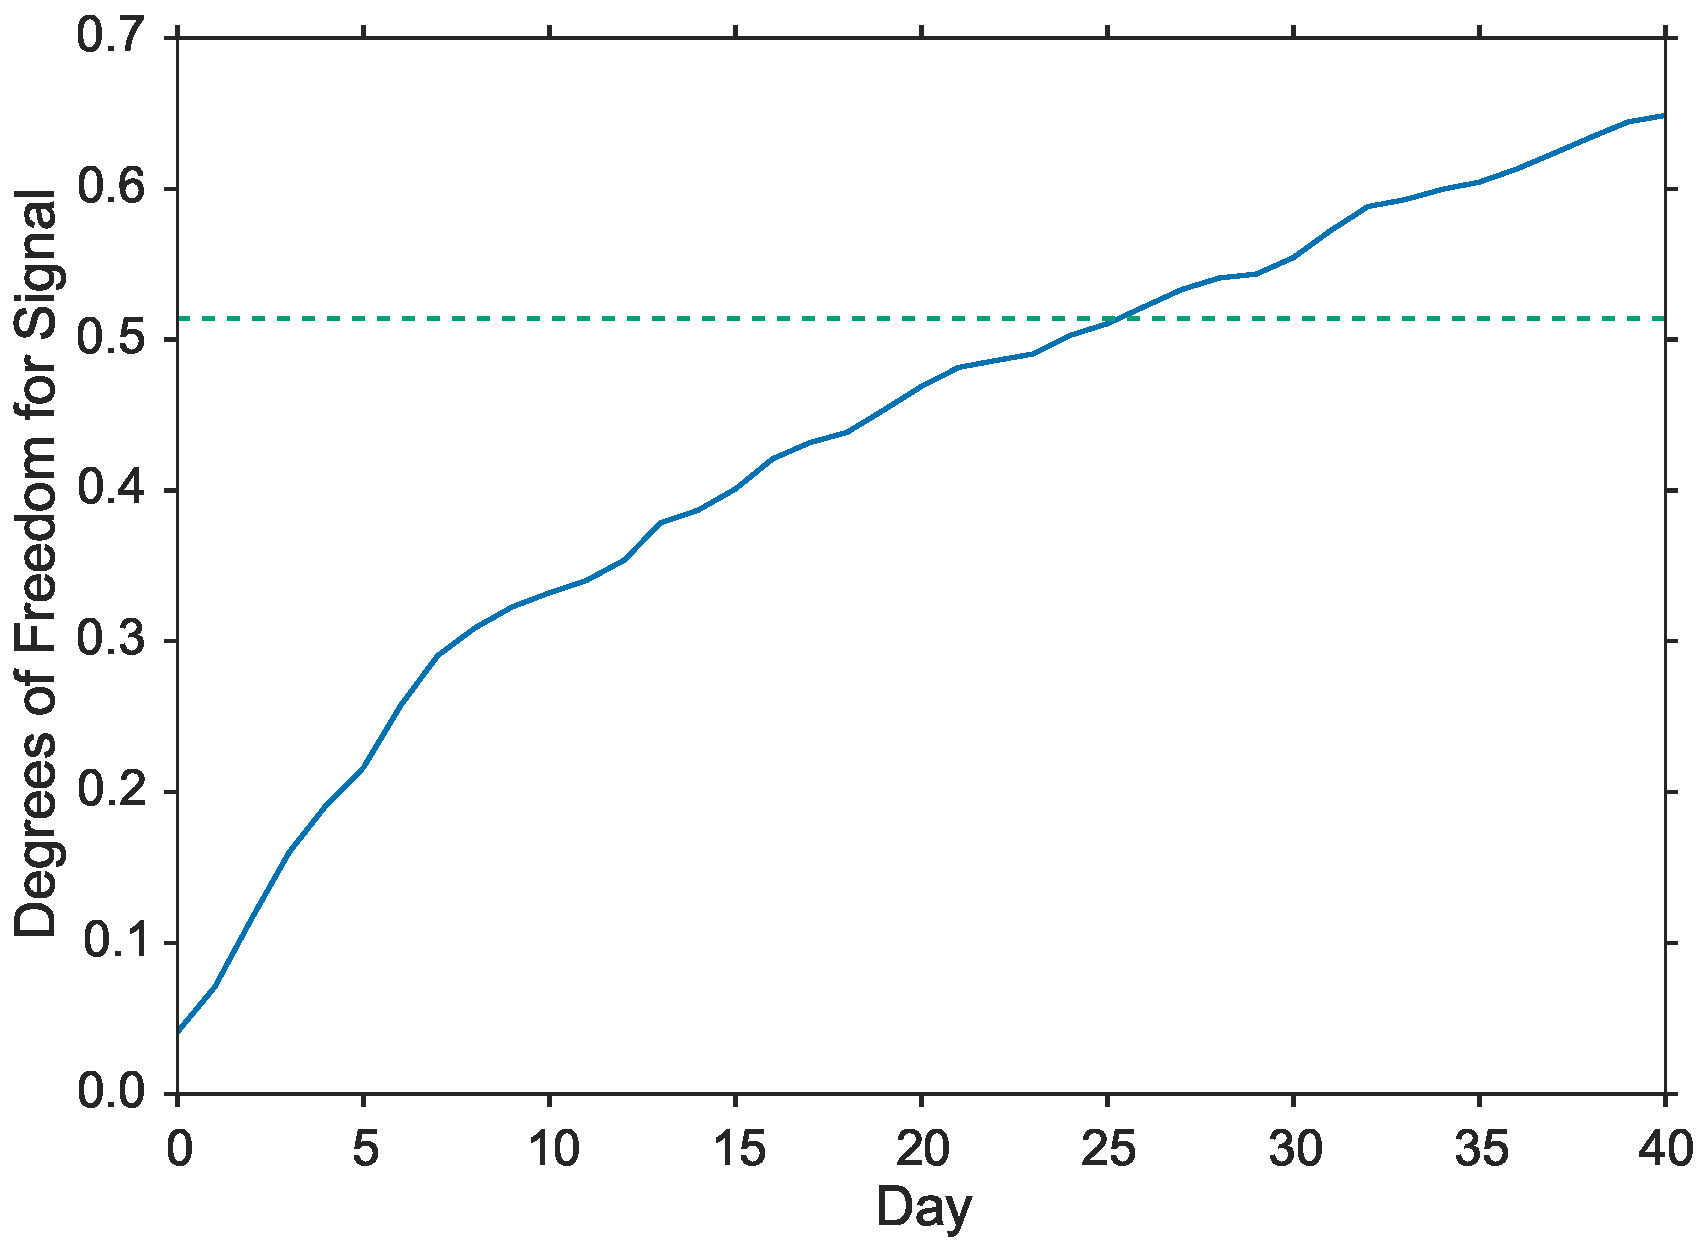
\includegraphics[width=\textwidth]{chapter/chapter5/dfs_succ_nee.pdf}
        \caption{\(dfs\) for successive NEE observations}
        \label{fig:dfs_succ_nee}
    \end{subfigure}
    \caption{Blue line: SIC and \(dfs\) for as successive NEE observations are added for 40 days from the \(1^{\text{st}}\) January 2007 using driving data from a pine stand in Oregon, green dotted line: SIC and \(dfs\) for a single summer observation of NEE made on \( 22^{\text{nd}} \) June 2007. }
    \label{fig:ic_succ_nee}
\end{figure}

\subsubsection{Effect of time correlations between observation errors on information content}

In chapter ({\color{red}ref. 1st results chapter}) we have investigated the effect of including correlations in time between observation errors on the results from data assimilation with DALEC2. We can see the effect on the analytic representation of information content for two successive observations of NEE when including an off-diagonal correlation term in the matrix \(\hat{\mathbf{R}}\). So that \(\hat{\mathbf{R}} = \hat{\mathbf{D}}\mathbf{C}\hat{\mathbf{D}}^{\text{T}}\), where \(\hat{\mathbf{D}}\) is the diagonal matrix of observation standard deviations and \(\mathbf{C}\) is a correlation matrix of the same shape. We then have
\begin{equation}
\hat{\mathbf{R}} =  \hat{\mathbf{D}}\mathbf{C}\hat{\mathbf{D}}^{\text{T}} =
\begin{pmatrix}
\sigma_{nee,o} & 0  \\
0 & \sigma_{nee,o}  \\
\end{pmatrix}
\begin{pmatrix}
1 & \rho  \\
\rho & 1  \\
\end{pmatrix}
\begin{pmatrix}
\sigma_{nee,o} & 0  \\
0 & \sigma_{nee,o}  \\
\end{pmatrix}
=
\begin{pmatrix}
\sigma_{nee,o}^{2} & \rho\sigma_{nee,o}^{2}  \\
\rho\sigma_{nee,o}^{2} & \sigma_{nee,o}^{2}  \\
\end{pmatrix},
\end{equation}
with \(0 \leq \rho < 1\).

We have not shown the analytic representation for the SIC here as it is too large. We instead use the symbolic Python package SymPy \citep{Joyner:2012:OSC:2110170.2110185} to plot the SIC for an increasing value of \(\rho\) in figure~\ref{fig:sic_corr_D1}.
\begin{figure}[ht]
	\centering
        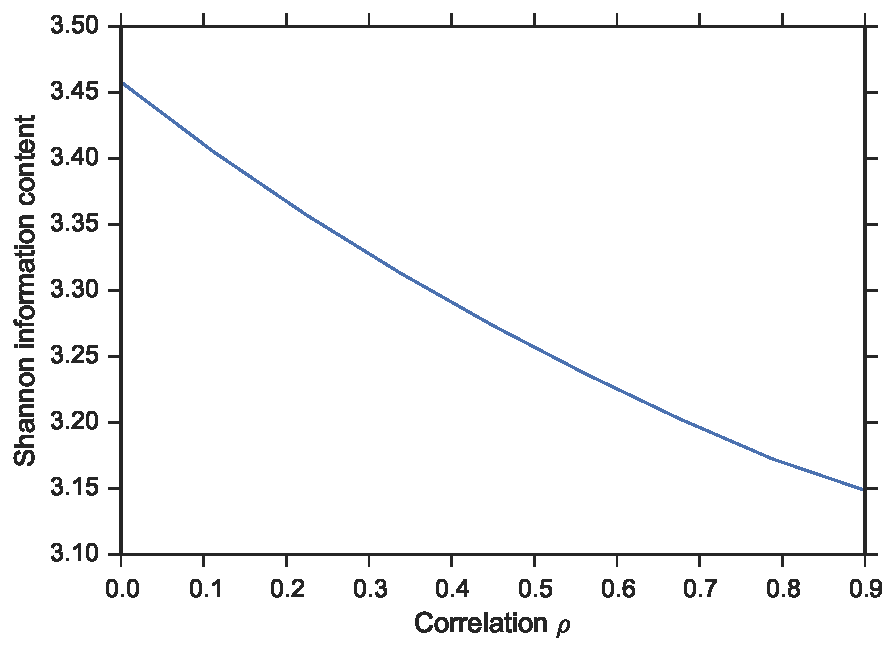
\includegraphics[width=0.5\textwidth]{chapter/chapter5/sic_corr_D1_nee.pdf}
    \caption{Shannon information content for two successive observations of NEE when a varying time correlation is included between observation errors.}
    \label{fig:sic_corr_D1}
\end{figure}
Figure~\ref{fig:sic_corr_D1} shows that as the size of time correlation \(\rho\) approaches 1 the information content in the two observations of NEE decreases. This decrease in information content makes sense as including the correlation in time is decreasing the amount of independent information we are assimilating. This result is also seen in \citet{jarvinen1999variational} where including a serial correlations between observation errors is shown to reduce the weight given to the mean of the observations in the assimilation (equivalent to inflating the variance of the observations). This also supports the results found in section ({\color{red}ref. 1st results chapter}) where we see that including correlations in time between observation errors reduces the fit to the assimilated observations in the analysis window.


\subsection{DALEC2 information content} \label{sec:D2_IC}%%%%%%%%%%%%%%%%%%%%%%%
\subsubsection{Information content in observations for DALEC2}
%SIC with D2 show same for single time, inf mat for evergreen and deciduous, difference in phenology has effect on info %content when model is involved successive obs less valuable than ones at start of the window. show col sums for inf mat.

In this section we repeat and extend some of the results we have found for information content with the DALEC1 state estimation case in section \ref{sec:D1_IC} to the DALEC2 joint parameter and state estimation case. This means we now have an augmented state of 23 elements (17 parameters and 6 state variables) as opposed to just the 5 state members for DALEC1. For this reason we no longer examine the analytic representations of information content but instead consider the information content calculated numerically for DALEC2. 

In section~\ref{sec:info_con_single_time} it was shown that for DALEC1 the information content for a single observation of NEE was dependent on temperature. From Figure~\ref{fig:neeSIC_temp_comp_D2} we can see that this is still the case for DALEC2. However the value of SIC is higher for DALEC2 in Figure~\ref{fig:neeSIC_temp_comp_D2} than for DALEC1 in Figure~\ref{fig:neeSIC_temp_comp} as the augmented state for the DALEC2 case also includes the parameters. This means that a single observation of NEE is giving us information about more elements of the state than for the DALEC1 state estimation case.

\begin{figure}[ht]
    \centering
    \begin{subfigure}[b]{0.45\textwidth}
        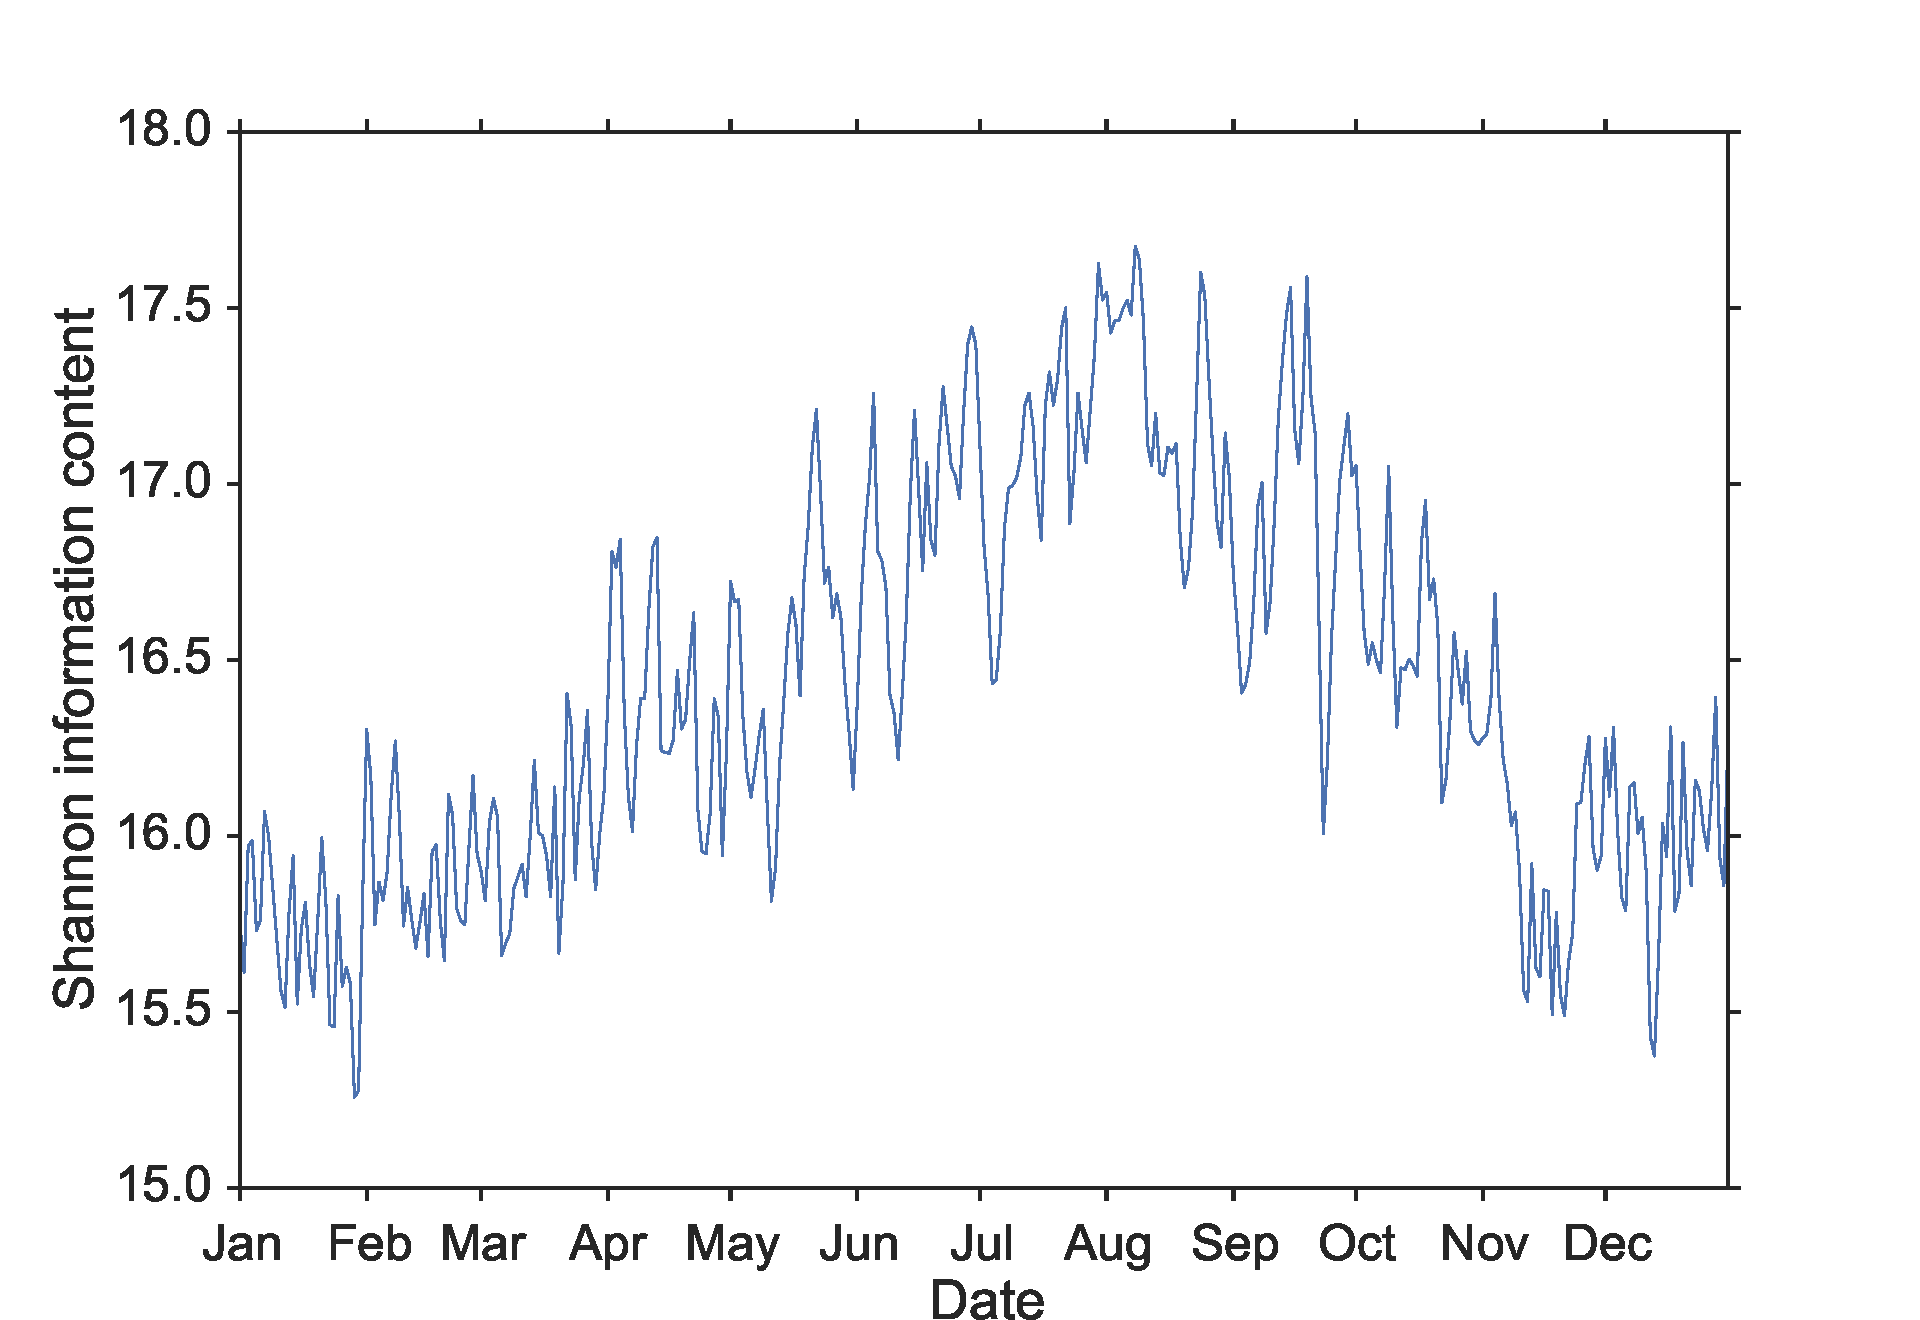
\includegraphics[width=\textwidth]{chapter/chapter5/oregon2007SICneeD2.pdf}
        \caption{SIC for single NEE observation}
        \label{fig:sic_nee_oregon2007_D2}
    \end{subfigure}%
    \begin{subfigure}[b]{0.45\textwidth}
        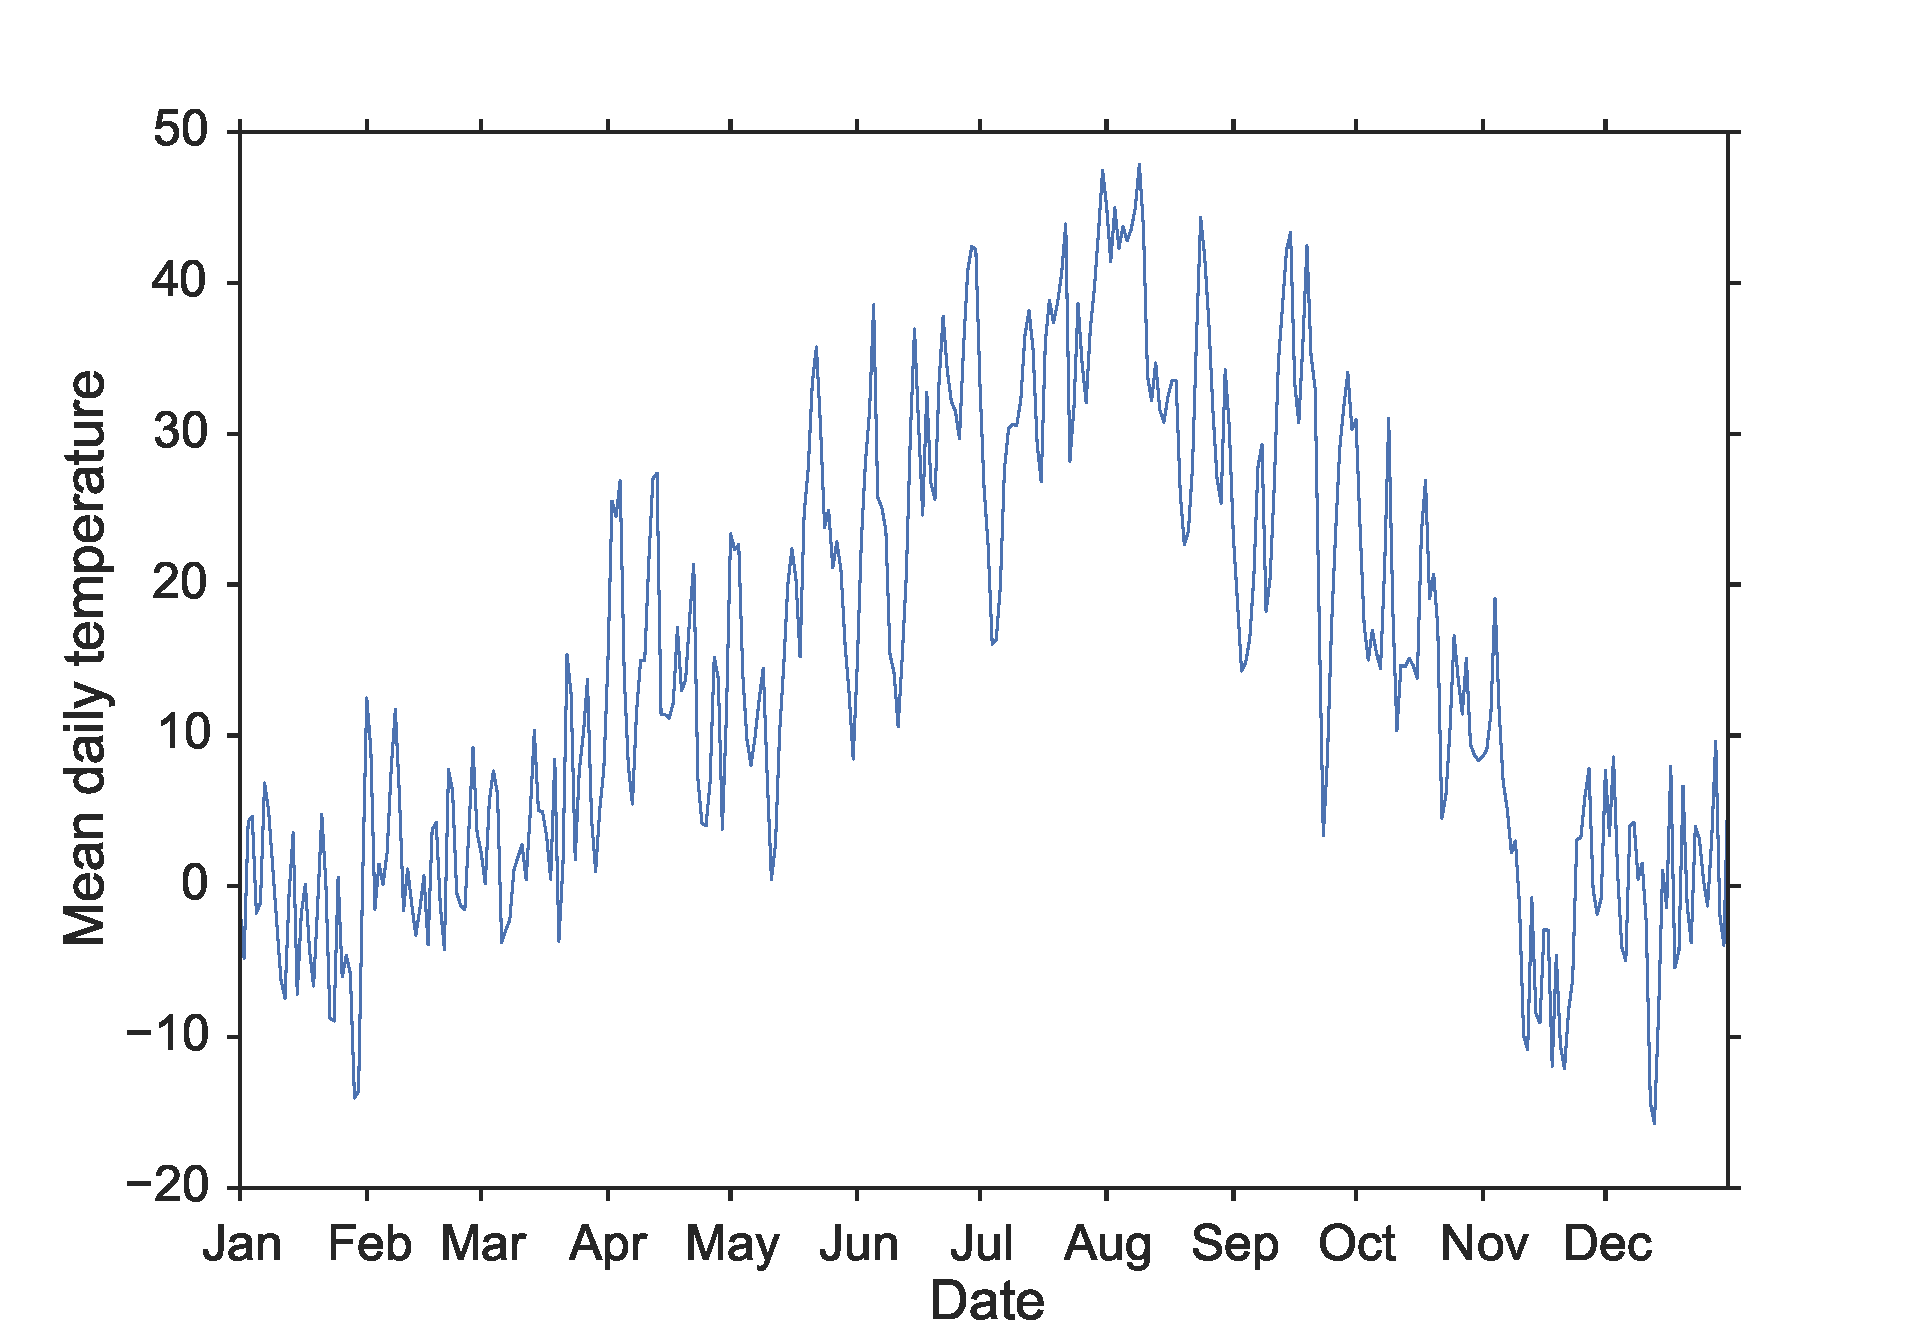
\includegraphics[width=\textwidth]{chapter/chapter5/oregon2007temp.pdf}
        \caption{Mean daily temperature for year's data}
        \label{fig:temp_nee_oregon2007_D2}
    \end{subfigure}
    \caption{SIC a single NEE observation changing throughout a year's window using driving data from a pine stand in Oregon taken in 2007 (left). Mean daily temperature for the same site and period (right).}
    \label{fig:neeSIC_temp_comp_D2}
\end{figure}

In figure~\ref{fig:neeSIC_temp_comp_D2} we have shown the information content varying for an evergreen forest site. As DALEC2 can also be parameterised and run for deciduous sites (with much work in this thesis being undertaken at Forest Research's deciduous study site, see section{\color{red}REF}) it is important to investigate the difference in information content between these cases. In order to visualise this difference, in figure~\ref{fig:inf_mats} we show the analysis sensitivity to observations or influence matrix \citep{Cardinali2004} as described in section~\ref{sec:inf_mat}, \(\textbf{S} = \textbf{K}^{T}\textbf{H}^{T}\), for a year's assimilation window with 365 observations of NEE. The influence matrix will depend on the initial augmented state we chose to linearise around, the driving data we use to run our model and the observations we specify for assimilation. In figure~\ref{fig:inf_mats} we use an initial augmented state optimised for the Alice Holt deciduous forest and an initial augmented state optimised for an evergreen site in Oregon, we then use the same yearly driving data for both states so that it is only the difference between the initial augmented states of the sites effecting the difference between the influence matrices.  

\begin{figure}[ht]
    \centering
    \begin{subfigure}[b]{0.46\textwidth}
        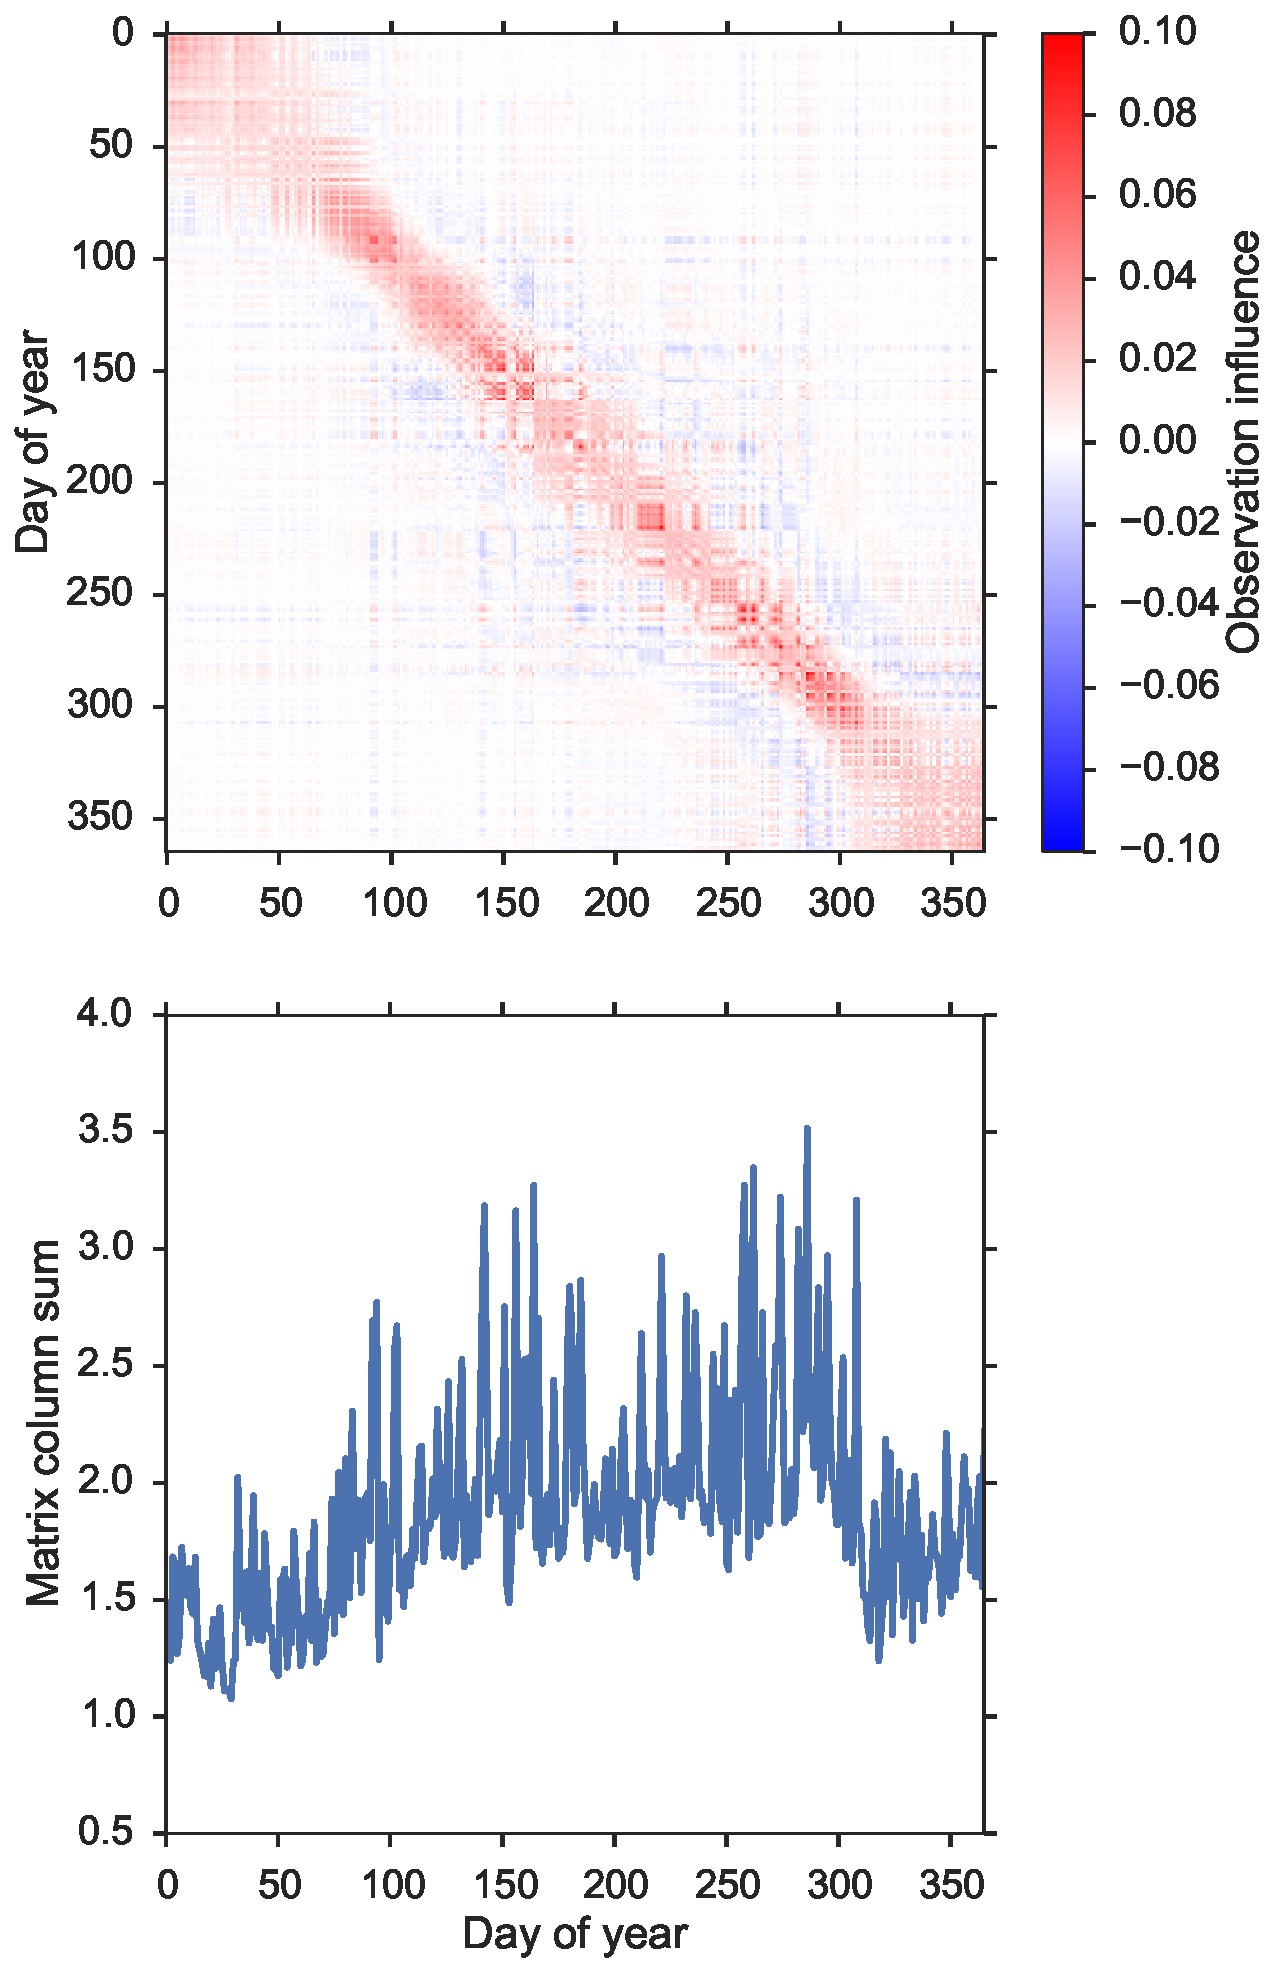
\includegraphics[width=\textwidth]{chapter/chapter5/inf_mat_sa.pdf}
        \caption{Alice Holt deciduous site}
        \label{fig:ah_inf_mat}
    \end{subfigure}%
    \begin{subfigure}[b]{0.46\textwidth}
        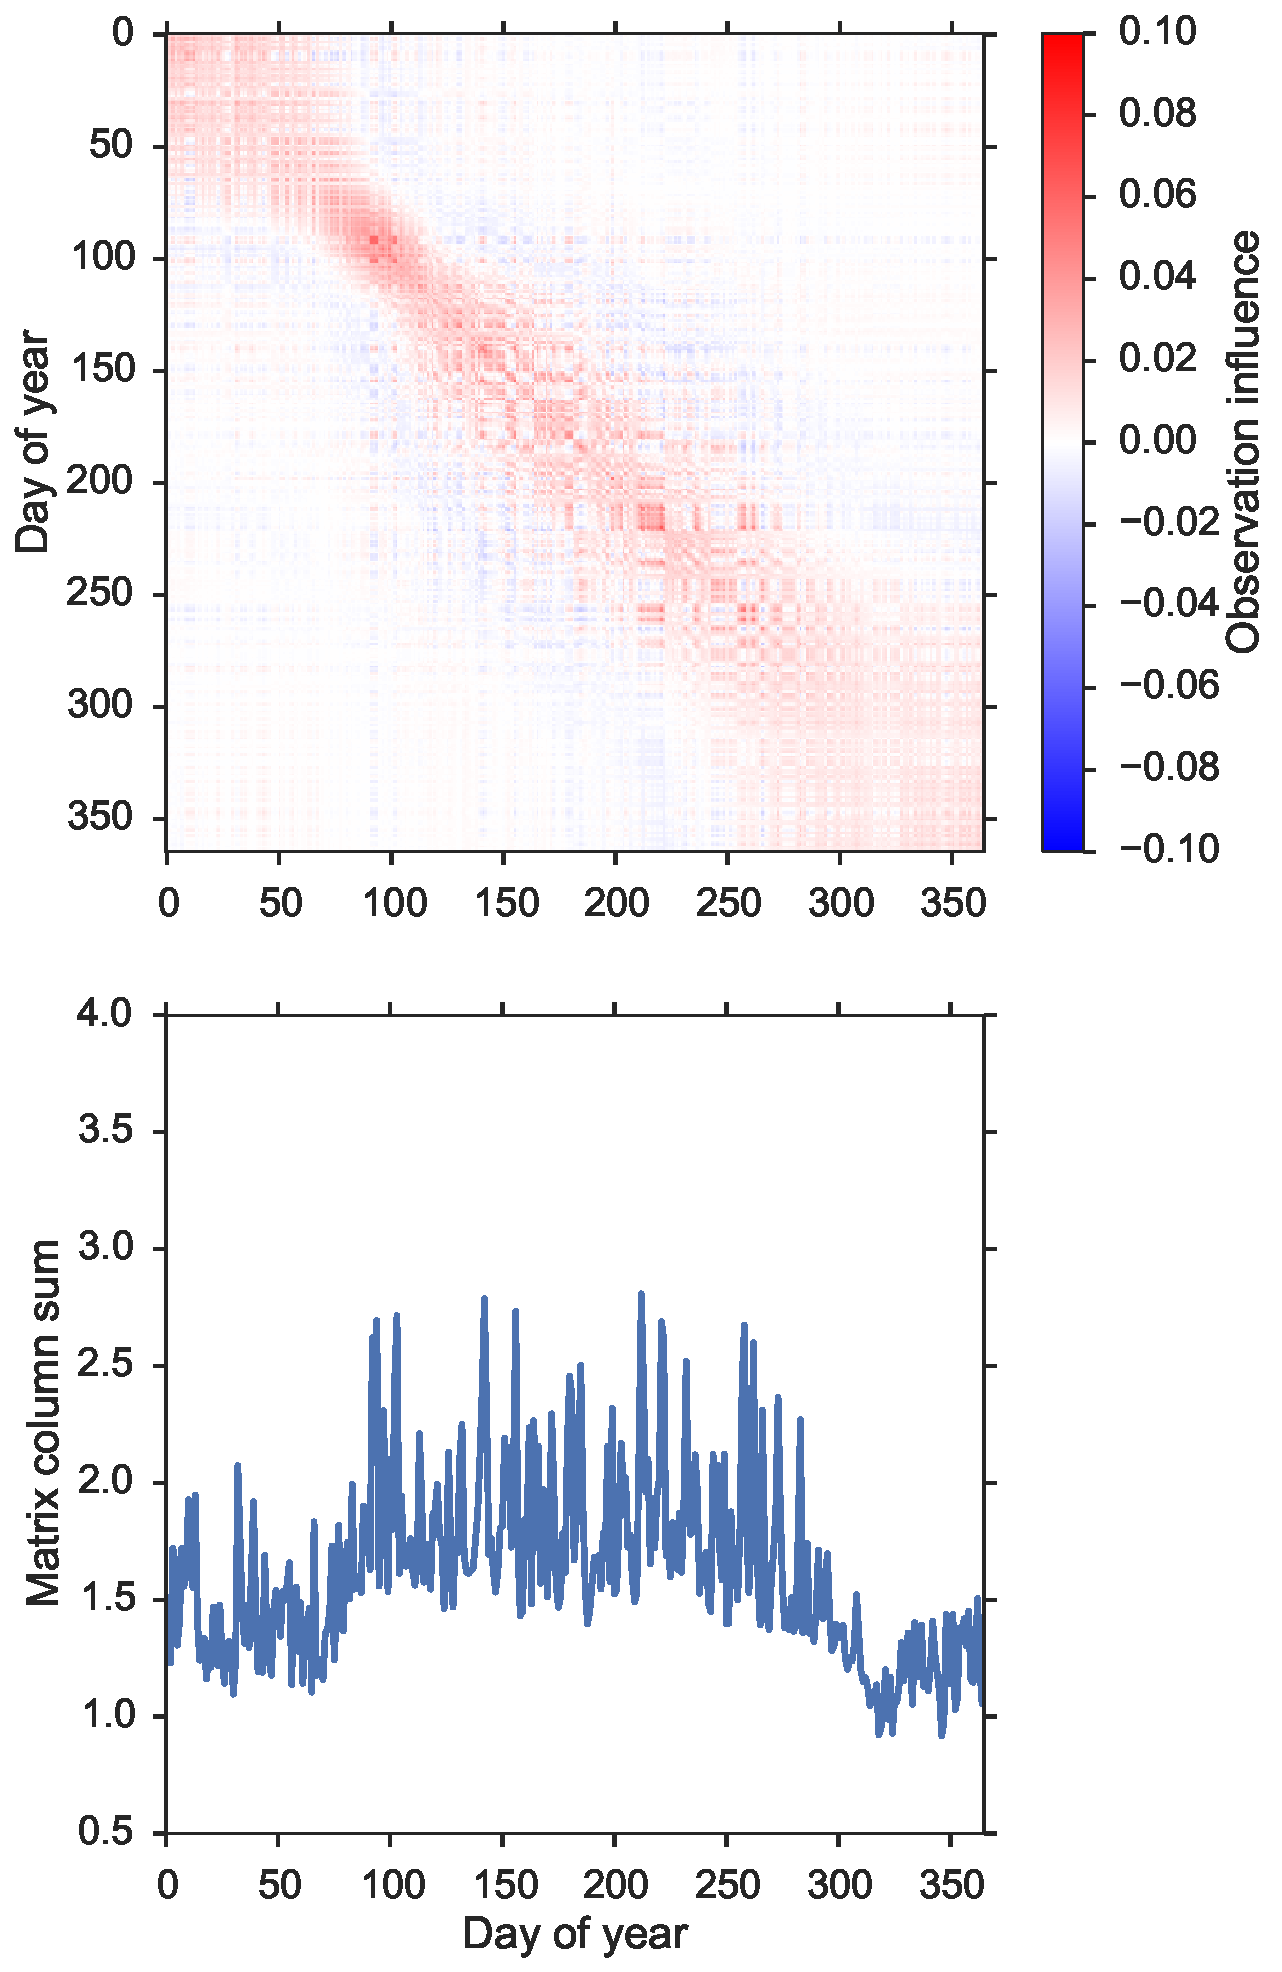
\includegraphics[width=\textwidth]{chapter/chapter5/inf_mat_so.pdf}
        \caption{Oregon evergreen site}
        \label{fig:oregon_inf_mat}
    \end{subfigure}
    \caption{Influence matrices and column absolute value sums as described in section~\ref{sec:inf_mat}, showing the sensitivity of the modelled observations to the assimilated observations for a year's assimilation window starting at the beginning of January with 365 observations of NEE.}
    \label{fig:inf_mats}
\end{figure}

From figure~\ref{fig:inf_mats} we can see that the influence of the assimilated observations of NEE is noticeably different between the deciduous and evergreen sites. However, in both cases at the beginning of the window there is a group of observations with similar influence. This makes sense as we are predicting the initial augmented state for DALEC2, so that observations closer to this initial state should have greater influence. 

For the deciduous site in figure~\ref{fig:ah_inf_mat} we have groups of observations with high influence from around day 125 to day 175 and from day 250 to day 300. We also have some high influence observations between these two groups. High influence observations between these two groups would be consistent with the results showing that NEE observations have higher information content with higher temperatures, as the period between day 175 and 250 contains days with higher mean temperatures. For the evergreen site in figure~\ref{fig:oregon_inf_mat}, although we have a group of observations at the beginning of the growing season with higher influence, we do not see a group of with the same high influence between day 250 to day 300 as with the deciduous case. We still see observations of high influence corresponding to times of higher temperatures for the evergreen case. 

\begin{figure}[ht]
    \centering
    \begin{subfigure}[b]{0.45\textwidth}
        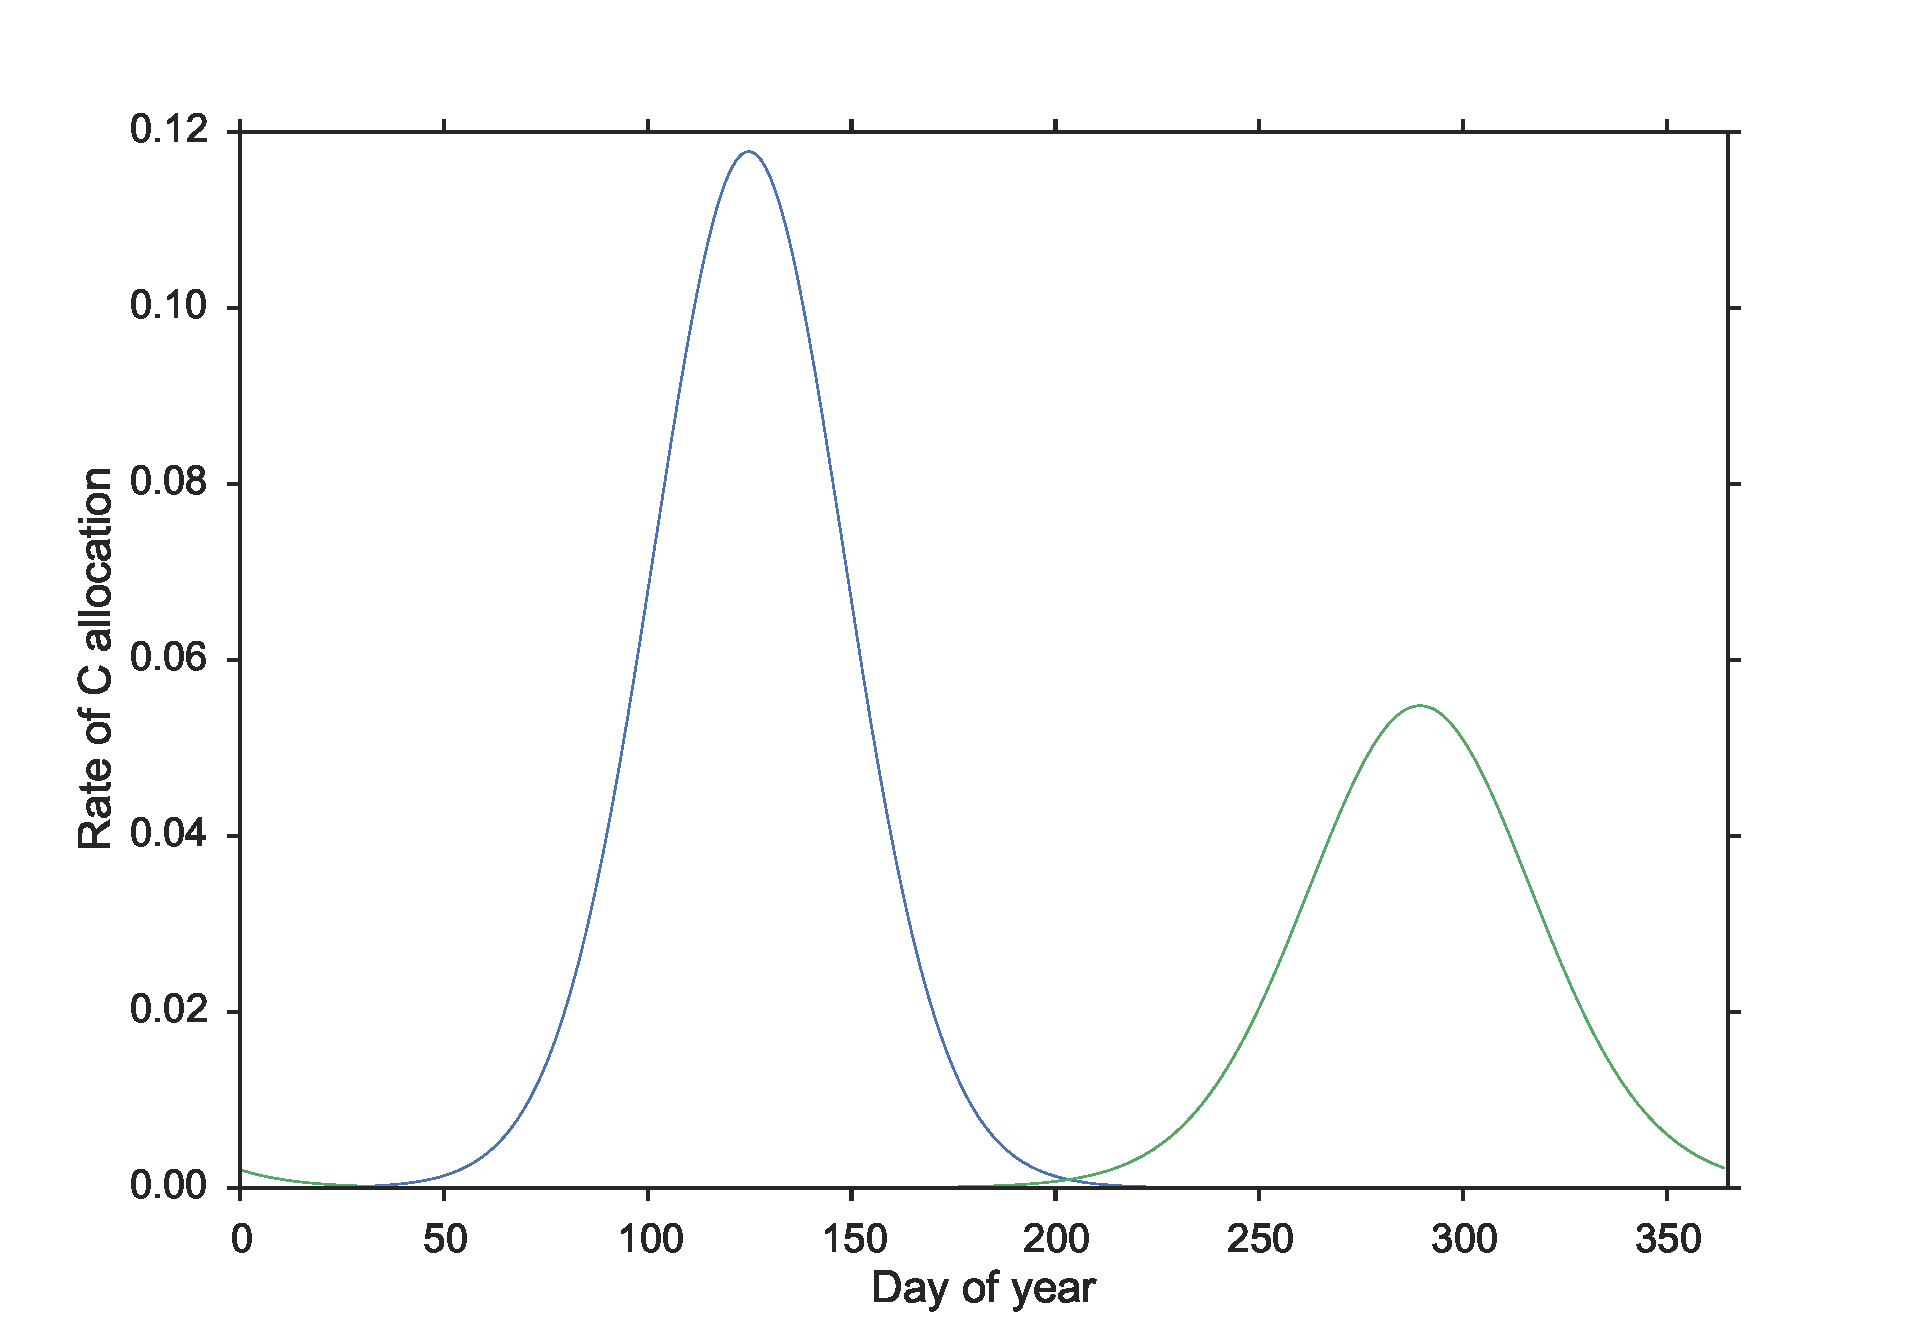
\includegraphics[width=\textwidth]{chapter/chapter5/ah_pheno.pdf}
        \caption{Alice Holt deciduous site}
        \label{fig:ah_pheno}
    \end{subfigure}%
    \begin{subfigure}[b]{0.45\textwidth}
        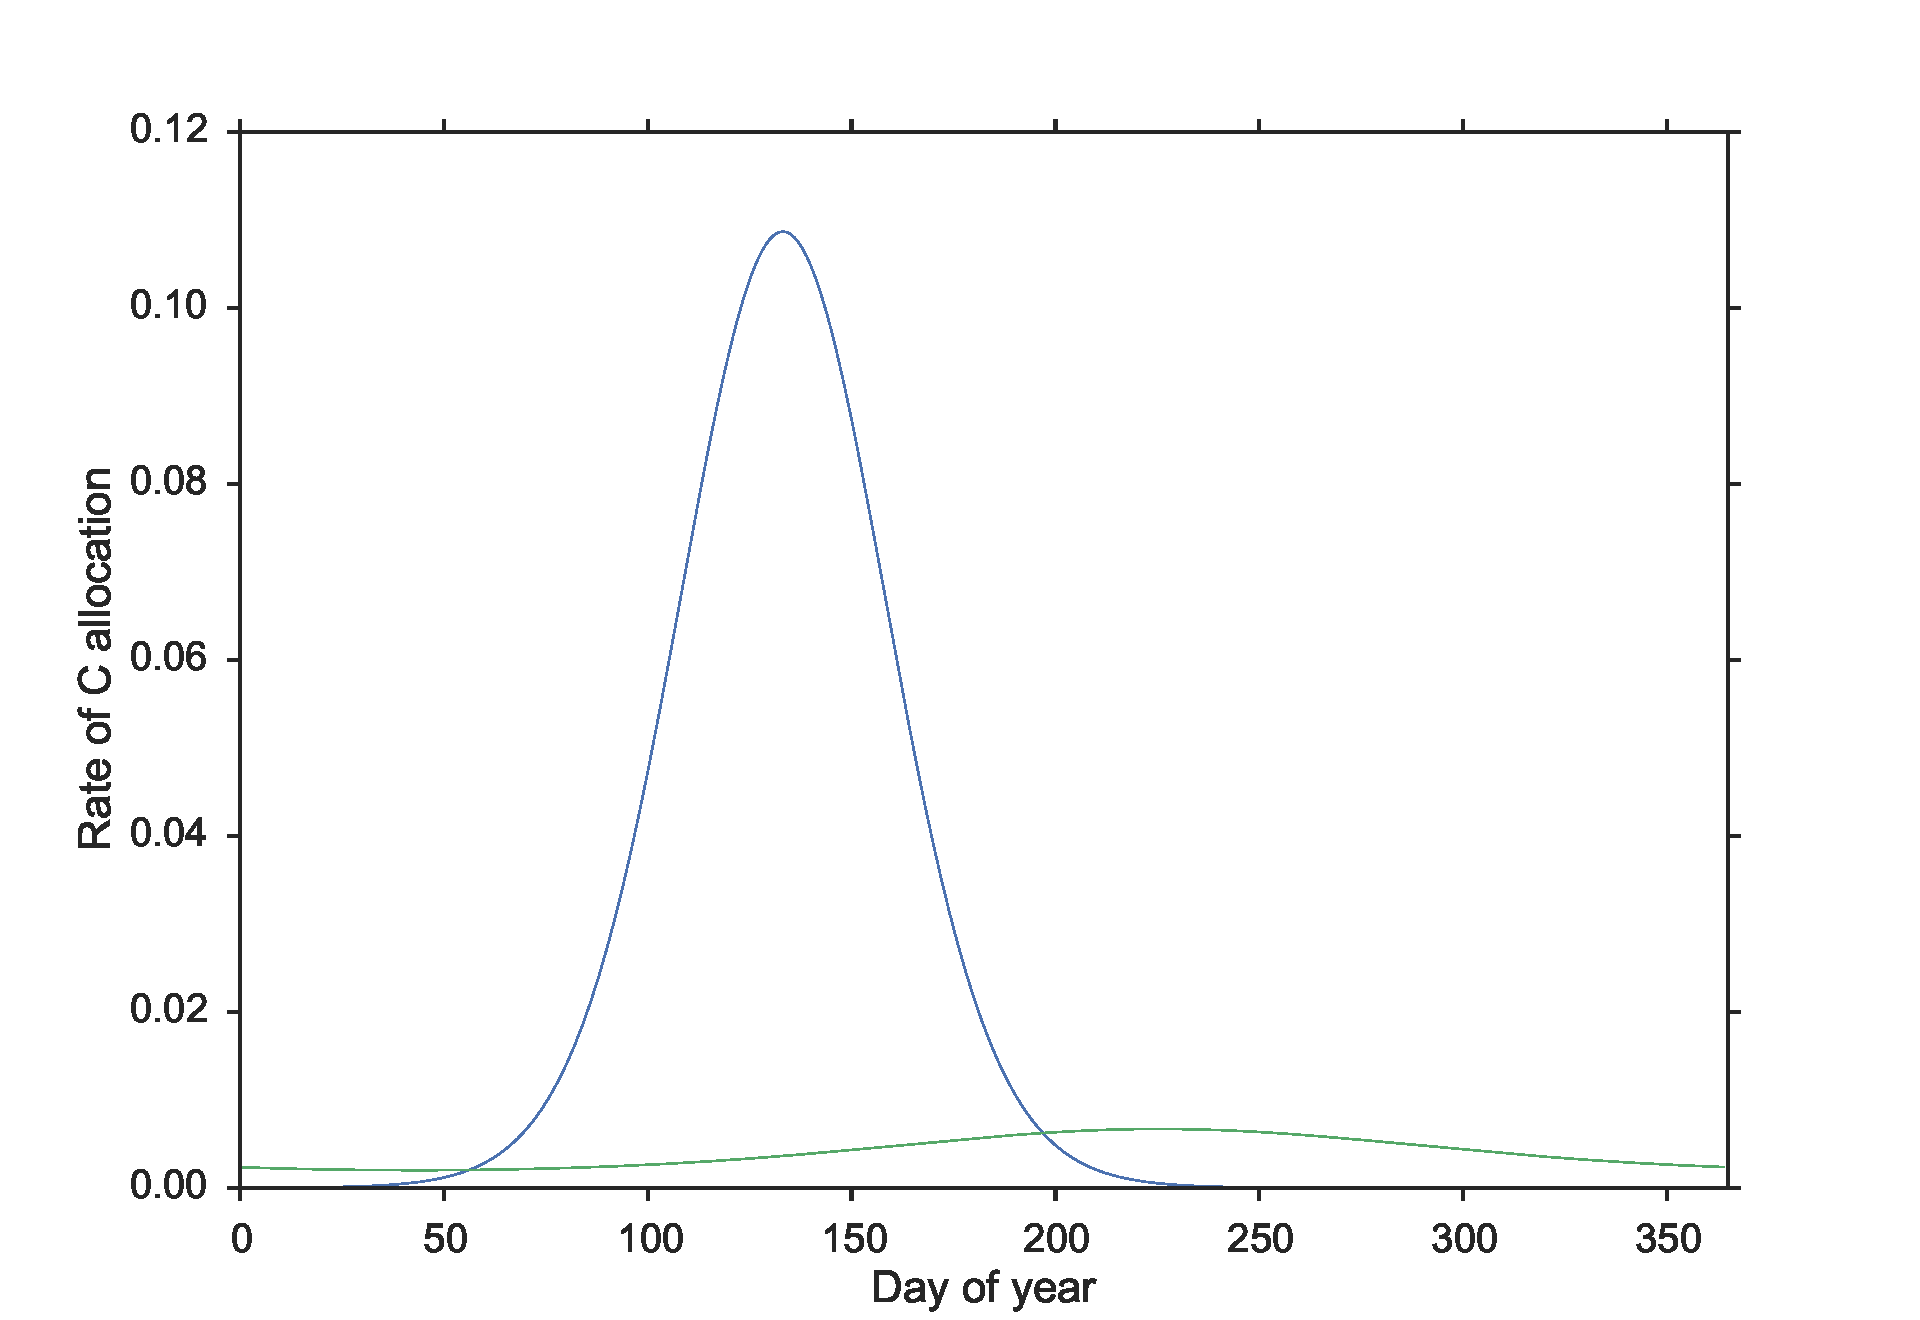
\includegraphics[width=\textwidth]{chapter/chapter5/oregon_pheno.pdf}
        \caption{Oregon evergreen site}
        \label{fig:oregon_pheno}
    \end{subfigure}
    \caption{Phenology of DALEC2 model for a deciduous and evergreen forest. Blue line: function controlling rate of leaf-on (\(\phi_{on}\)), green line: function controlling rate of leaf-off (\(\phi_{off}\)).}
    \label{fig:D2_pheno}
\end{figure}

In order to further investigate these groups of high influence observations we show the phenology functions controlling the rate of leaf-on and leaf-off for the DALEC2 model in figure~\ref{fig:D2_pheno}. The description of phenology is the main difference between the more simplistic, evergreen only, DALEC1 and DALEC2 which can be parameterised for both deciduous and evergreen sites. It is logical that this is what is causing the difference in information content between the models and between the different sites. In figure~\ref{fig:D2_pheno} we see that the function controlling leaf-off for the deciduous site has a far larger peak than that of the evergreen site. This is expected as the deciduous site will drop all of its leaves at the end of the season. In both cases the forest puts most effort into putting on new leaves at the start of the growing season. This highlights the fact that the NEE for a deciduous site is highly controlled by phenology, as the forest cannot photosynthesise without leaves. Therefore the observations of NEE that help to constrain the phenology of the site should have a higher influence, as seen in figure~\ref{fig:ah_inf_mat}. Conversely for an evergreen site NEE is driven less by phenology and more by the climatic driving data. Seeing a greater relationship between temperature and information content  for an evergreen site consequently makes sense and this can be seen in figure~\ref{fig:oregon_inf_mat}.



\subsubsection{Effect of time correlations on observation information content}

In section~\ref{sec:D1_succ_obs} it was shown that, for the analytic DALEC1 case, when assimilating two successive observations of NEE the SIC decreased when including a correlation in time between NEE observation errors. It was noted that this was consistent with results found in section ({\color{red}ref. 1st results chapter}) where including correlations between observation errors in time reduced the weight of the observations in the assimilation, in turn reducing the issue of overfitting to the assimilated observations. In figure~\ref{fig:sic_corr_D2} we repeat the experiment in section~\ref{sec:D1_succ_obs} but for DALEC2 with the year's worth of NEE observations assimilated in section ({\color{red}ref. 1st results chapter}), in order to verify that including a correlation in time reduces the information content in assimilated observations. 
\begin{figure}[ht]
	\centering
        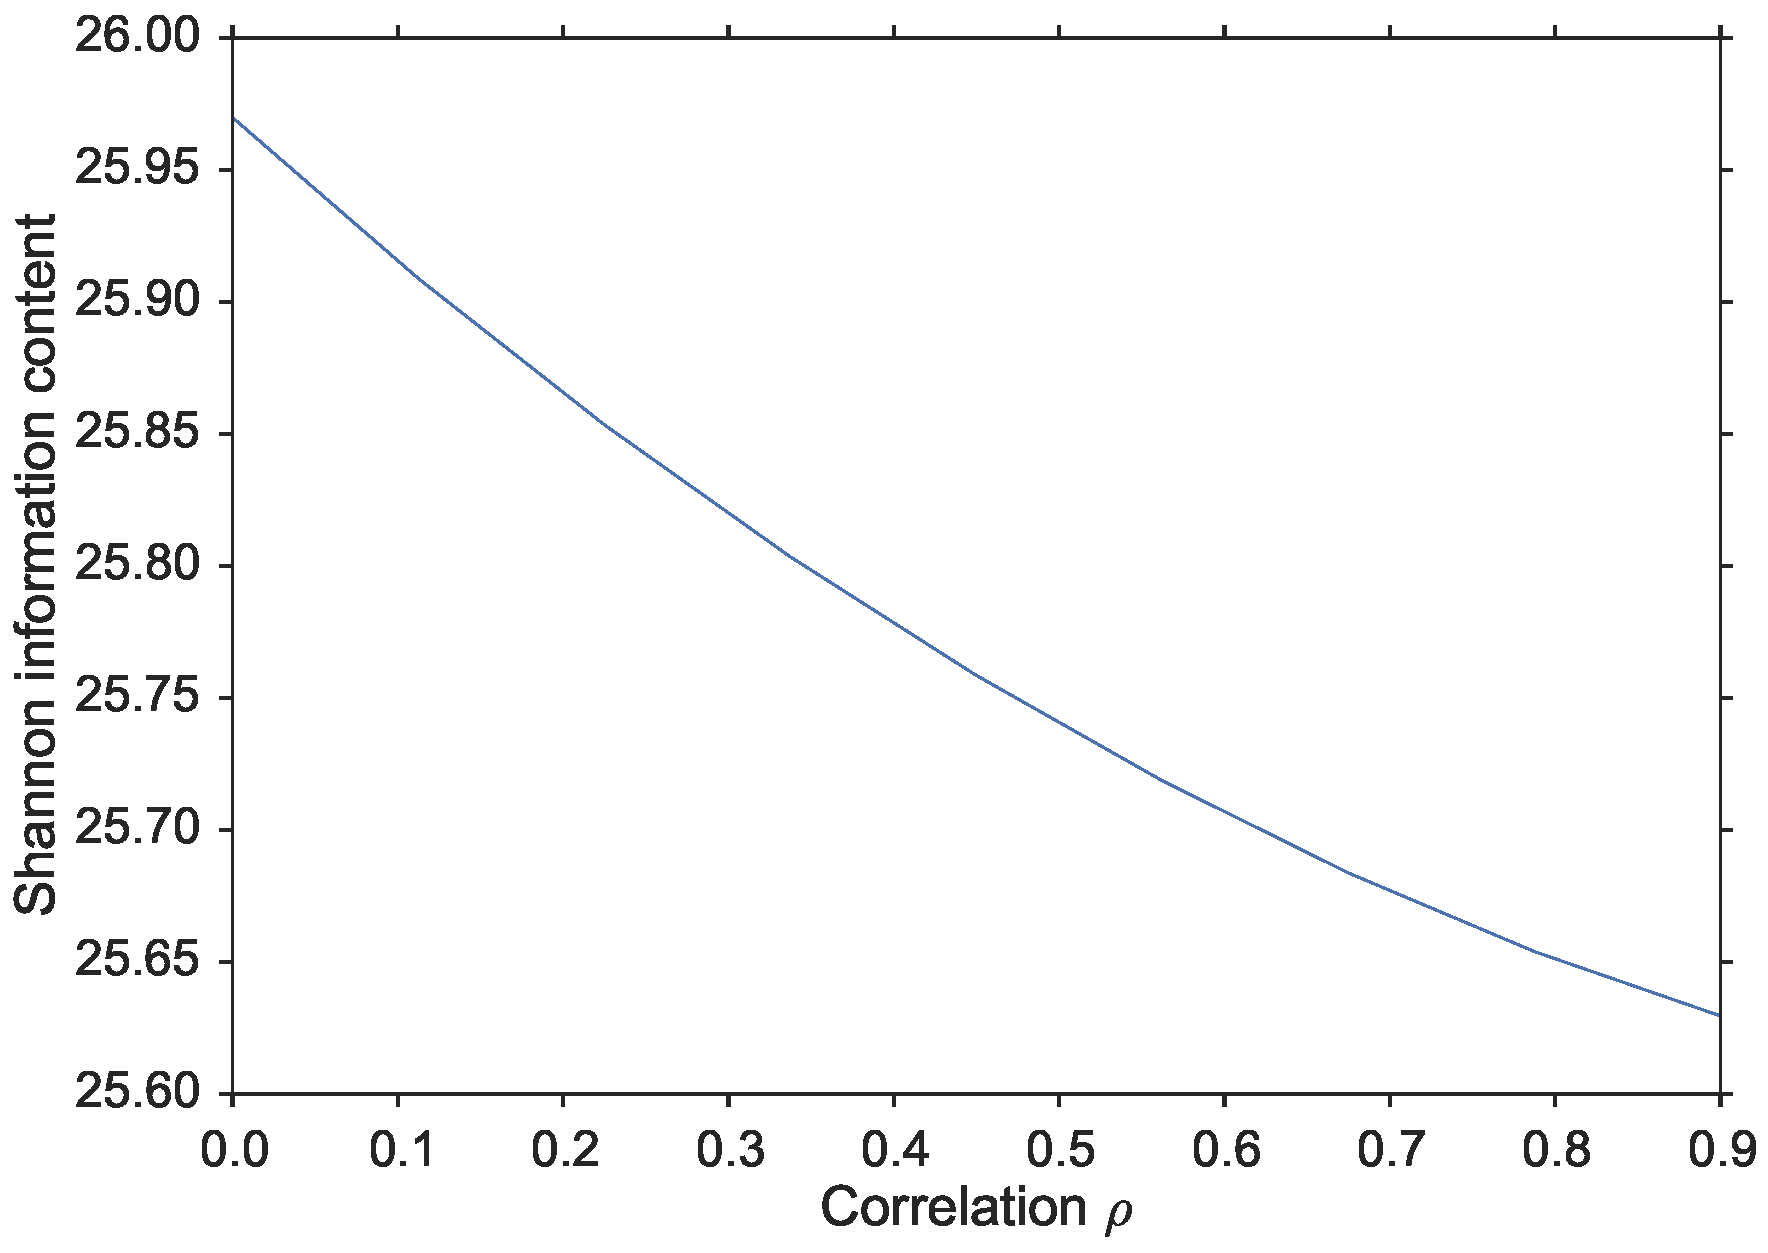
\includegraphics[width=0.5\textwidth]{chapter/chapter5/sic_corr_D2_nee.pdf}
    \caption{Shannon information content for 67 observations of NEE taken throughout a year's assimilation window when a varying time correlation is included between observation errors.}
    \label{fig:sic_corr_D2}
\end{figure}
From figure~\ref{fig:sic_corr_D2} we see that we have similar results as in figure~\ref{fig:sic_corr_D1} where the information content in our observations decreases as we increase the time correlation between the assimilated observation errors. However, in figure~\ref{fig:sic_corr_D2} we have a higher value of SIC as we are assimilating many more observations than in figure~\ref{fig:sic_corr_D1}. In figure~\ref{fig:sic_corr_D2} we have used the same correlation function as in section ({\color{red}ref. 1st results chapter}) to create a correlated matrix \(\hat{\textbf{R}}\) and then varied the magnitude of the included correlation, \(\rho\). The decreasing information content with an increasing correlation between observation errors in time supports the results in section~\ref{sec:D1_succ_obs} and section ({\color{red}ref. 1st results chapter}). This is also consistent with the results of  \citet{jarvinen1999variational} where including correlations between observation errors in time is shown to reduce the weight given to the mean of the observations in the assimilation (equivalent to inflating the variance of the observations).

%\subsubsection{Increasing available information by day/night sampling of NEE}

%In previous work we have averaged the 48 half-hourly measurements of NEE in a day to find a value for total daily NEE. This is because we are working with a model that has a daily time step and thus need to assimilate observations at the same temporal resolution. In REF Richardson et al... it is shown that the assimilation of NEE averaged half daily (so that we have observations of daytime NEE and nighttime NEE) can improve data assimilation results and the model partitioning between GPP and RT. This is because nighttime NEE is equal to RT as no photosynthesis occurs at night.

%In this section we will show how we can assimilation day and nighttime NEE without making any modifications to our model. We do this by creating two modified observation operators to relate our model state and parameters at time \(i\) to both daytime and nighttime NEE at time \(i\). We still use the DALEC2 model here but this technique is applicable to any other ecosystem carbon model. Here we show a set of twin experiments to illustrate how assimilating NEE twice daily can be beneficial over assimilating a single value of total daily NEE. The main benefit coming from the fact that we have a greater number of observations after processing the raw eddy covariance data. This is because we are averaging over fewer half-hourly observations so have a lower probability of gaps appearing in our averaging period. This means we throw away less observations than we would when averaging over the total 48 half-hourly observations of NEE in a day.

\section{Conclusions}

In this chapter we have investigated both the observability and information content given the observations available to us. In section~\ref{sec:D1observability} and section~\ref{sec: D2_observability} we have shown that for both DALEC1 and DALEC2 we have an observable system with the available observations, in this case NEE. An observable system in this case means that for data assimilation we can construct a locally unique solution from the observational information alone. 

In section~\ref{sec:D1_IC} we have seen that for the DALEC1 evergreen case the information content in observations of NEE is largely dependent on temperature, with higher temperatures meaning higher information content. This is important for informing planned maintenance or down time at flux tower sites measuring NEE. This dependance of information content on temperature is also seen for observations of ground respiration and total ecosystem respiration. When assimilating additional observations at the same time alongside NEE we have found that most information is added when the additional observation provides an orthogonal constraint to that of NEE. This is the case for root carbon (\(C_{roo}\)) and woody biomass carbon (\(C_{woo}\)), with the European Space Agency BIOMASS mission being launched soon this should add valuable information to current data assimilation schemes. When using DALEC1 and assimilating successive observations in time it was shown that as observations are added further away from the initial state their impact is decreased. For two successive observation of NEE it was also shown that including a correlation in time between observation errors decreases the information content in the assimilated observations. This is consistent with results found in ({\color{red} ref. 1st results chapter}) where including correlations in time between observation errors reduces overfitting to the assimilated observations.

In section~\ref{sec:D2_IC} we again see the temperature dependence of information content in observations of NEE for DALEC2. However, for DALEC2 we also have varying information content based on the type of ecosystem we are observing. For a deciduous forest site we see that as well as temperature the information content in observations of NEE is strongly dependent on the time of growing season. Observations made at the time of leaf-on and leaf-off have higher influence on the results of the assimilation. This makes physical sense as for a deciduous ecosystem NEE is highly controlled by phenology, as the forest cannot photosynthesise without leaves. Therefore the observations of NEE that help to constrain the phenology of the site should have a higher influence. For an evergreen forest site we see much less dependence on phenology and have a greater relationship between temperature and information content. We again see similar results as in section~\ref{sec:D1_IC} when including correlations in time between observation errors, with an increasing correlation, \(\rho\), reducing the information content in the assimilated observations.


\chapter{Investigating the role of prior and observation error correlations}
\label{chap:error_corrs}
%Chapter 6

\section{Abstract}
Efforts to implement variational data assimilation routines with functional ecology models and land surface models have been limited, with sequential and Markov chain Monte Carlo data assimilation methods being prevalent. When data assimilation has been used with models of carbon balance, prior or ``background" errors (in the initial state and parameter values) and observation errors have largely been treated as independent and uncorrelated. Correlations between background errors have long been known to be a key aspect of data assimilation in numerical weather prediction. More recently, it has been shown that accounting for correlated observation errors in the assimilation algorithm can considerably improve data assimilation results and forecasts. In this paper we implement a Four-Dimensional Variational data assimilation (4D-Var) scheme with a simple model of forest carbon balance, for joint parameter and state estimation and assimilate daily observations of Net Ecosystem $\text{CO}_{2}$ Exchange (NEE) taken at the Alice Holt forest $\text{CO}_2$ flux site in Hampshire, UK. We then investigate the effect of specifying correlations between parameter and state variables in background error statistics and the effect of specifying correlations in time between observation errors. The idea of including these correlations in time is new and has not been previously explored in carbon balance model data assimilation. In data assimilation, background and observation error statistics are often described by the background error covariance matrix and the observation error covariance matrix. We outline novel methods for creating correlated versions of these matrices, using a set of previously postulated dynamical constraints to include correlations in the background error statistics and a Gaussian correlation function to include time correlations in the observation error statistics. The methods used in this paper will allow the inclusion of time correlations between many different observation types in the assimilation algorithm, meaning that previously neglected information can be accounted for. In our experiments we assimilate a single year of NEE observations and then run a forecast for the next 14 years. We compare the results using our new correlated background and observation error covariance matrices and those using diagonal covariance matrices. We find that using the new correlated matrices reduces the root mean square error in the $14$ year forecast of daily NEE by $44\%$ decreasing from $4.22~\text{gCm}^{-2}\text{day}^{-1}$ to $2.38~\text{gCm}^{-2}\text{day}^{-1}$.     

\section{Introduction} \label{sec:intro}

%\subsection{Tree blurb}
The land surface and oceans are responsible for removing around half of all human emitted carbon-dioxide from the atmosphere and therefore mediate the effect of anthropogenic induced climate change. Terrestrial ecosystem carbon uptake is the least understood process in the global carbon cycle \citep{ciais2014carbon}. It is therefore vital that we improve understanding of the carbon uptake of terrestrial ecosystems and their response to climate change in order to better constrain predictions of future carbon budgets. Observations of the Net Ecosystem Exchange (NEE) of CO$_{2}$ between terrestrial ecosystems and the atmosphere are now routinely made at flux tower sites world-wide, at sub-hourly resolution and covering multiple years \citep{baldocchi2008turner}, providing a valuable resource for carbon balance model validation and data assimilation.

%\subsection{DA paragraph}
Data assimilation is the process of combining a mathematical model with observations in order to improve the estimate of the state of a system. Data assimilation has successfully been used in many applications to significantly improve model state and forecasts. Perhaps the most important application has been in numerical weather prediction where data assimilation has contributed to the forecast accuracy being increased at longer lead times, with the four day forecast in 2014 having the same level of accuracy as the one day forecast in 1979 \citep{bauer2015quiet}. This increase in forecast skill is obviously not solely due to data assimilation but also increased quality and resolution of observations along with improvements in model structure, however the introduction and evolution of data assimilation has played a large part \citep{dee2011era}. The current method implemented at many leading operational numerical weather prediction centres is known as Four-Dimensional Variational data assimilation (4D-Var) \citep{QJ:QJ2652, QJ:QJ2054}, which has been shown to be a significant improvement over its predecessor three-dimensional variational data assimilation \citep{lorenc2005does}. Variational assimilation techniques minimise a cost function to find the optimal state of a system given all available knowledge of errors in the model and observations. The minimisation routine typically requires the derivative of the model which can sometimes prove difficult to calculate. Using techniques such as automatic-differentiation \citep{renaud1997automatic} can reduce the time taken to implement the derivative of a model. 

In numerical weather prediction data assimilation has been predominately used for state estimation whilst keeping parameters fixed. This is because numerical weather prediction is mainly dependent on the initial state with model physics being well understood. Ecosystem carbon cycle models are more dependent on finding the correct set of parameters to describe the ecosystem of interest \citep{luo2015predictability}. This is possibly why Monte Carlo Markov chain (MCMC) data assimilation methods have been used more with ecosystem carbon cycle models. Smaller ecosystem models are much less computationally expensive to run than large numerical weather prediction models, meaning that MCMC methods (requiring many more model runs than variational assimilation methods) are more easily implemented. For larger scale and more complex ecosystem models variational methods represent a much more computationally efficient option for data assimilation. Variational data assimilation can be used for joint parameter and state estimation by augmenting the state vector with the parameters \citep{navon1998practical}. By including the parameters in the state vector we must also specify error statistics and error correlations for them. \citet{smith2009variational} show that the prescription of these error statistics and their correlations can have a significant impact on parameter-state estimates obtained from the assimilation.

%\subsection{DALEC and ecosystem models with data assimilation (draw out gaps):}
Many different observations relevant to the carbon balance of forests have now been combined with functional ecology models, using data assimilation, in order to improve our knowledge of ecological systems \citep{zobitz2011primer, fox2009reflex, richardson2010estimating, Quaife2008, Zobitz2014, Niu2014}. Two such models that have been used extensively with data assimilation are the Data Assimilation Linked Ecosystem Carbon (DALEC) model \citep{williams2005improved} and the Simplified Photosynthesis and Evapo-Transpiration (SIPNET) model \citep{braswell2005estimating}. Nearly all data assimilation routines built with these models have used sequential and Monte Carlo Markov chain (MCMC) data assimilation methods with the exception of a variational routine being implemented for DALEC by \citet{delahaies2013regularization}. There have been examples of global land surface models being implemented with variational methods such as the ORganizing Carbon and Hydrology In Dynamic EcosystEms model (ORCHIDEE) \citep{Krinner2005} and the Biosphere Energy Transfer HYdrology scheme (BETHY) in a Carbon Cycle Data Assimilation System (CCDAS) \citep{Kaminski2013}. These examples have mainly been used to assimilate data from satellite and atmospheric $\text{CO}_{2}$ observations with only a few cases where site level data has also been assimilated \citep{Verbeeck2011, Bacour2015}. 

Forest carbon balance model parameters are often determined in advance of using the model for forecasting by calibration of the model against observations \citep{richardson2010estimating, Bloom2015}. Here we take the alternative approach of concurrent state-parameter estimation. A key difference between the joint state-parameter estimation approach and a priori calibration is the way that the observational data is used. Pre-calibration approaches train the model against historical data and so become infeasible when there is a lack of sufficient observational information prior to the model forecast period. Joint state-parameter estimation methods have the advantage that observations could be used as they arrive in real time, by sequential assimilation cycling. This approach also gives the possibility of adapting to changes in the forest (e.g., tree thinning, fires etc.) that may change the parameter values over time. 

Background errors (describing our knowledge of error in prior model estimates before data assimilation) and observation errors have largely been treated as uncorrelated and independent in ecosystem model data assimilation schemes. In 3D and 4DVar schemes background and observation errors are represented by the error covariance matrices \textbf{B} and \textbf{R} respectively. The off-diagonal elements of these matrices indicate the correlations between errors in the parameter and state variables for \textbf{B} and the correlations between observation errors for \textbf{R}. In the assimilation, the off-diagonal terms in the \textbf{B} matrix act to spread information between the state and augmented parameter variables \citep{kalnay2003atmospheric}. This means that assimilating observations of one state variable can act to update different state and parameter variables in the assimilation when correlations are included in \textbf{B}. In 4D-Var the \textbf{B} matrix is propagated implicitly by the forecast model, so that even a propagated diagonal \textbf{B} matrix can develop correlations throughout an assimilation window. These correlations will only be in the propagated \textbf{B} matrix, with the \textbf{B} matrix valid at the initial time remaining unchanged. Including correlations in \textbf{B} has been shown to significantly improve data assimilation results in numerical weather prediction \citep{bannister2008review}. 

Including correlations between observation errors has only started to be explored recently in numerical weather prediction, with \textbf{R} still often treated as diagonal \citep{Stewart2013}. Including some correlation structure in \textbf{R} has been shown to improve forecast accuracy \citep{weston2014accounting}. Currently the correlations included in \textbf{R} have been mainly between observations made at the the same time rather than correlations between observations throughout time. When assimilating observations, data streams with many more observations can have a greater impact on the assimilation than those with fewer observations. In \citet{richardson2010estimating} this problem is discussed when assimilating large numbers of NEE observations along with smaller numbers of leaf area index and soil respiration observations. To address this problem Richardson et al. uses a cost function that calculates the product of the departures from the observations rather than a cost function which sums these departures, giving a relative rather than absolute measure of the goodness-of-fit to the observations. This problem is also encountered in \citet{Bacour2015} when assimilating daily eddy covariance data with weekly observations of the FrAction of Photosynthetically Active Radiation (FAPAR). In \citet{Bacour2015} the error in observations of FAPAR is divided by two in order to give these less frequent observations more weight in the assimilation algorithm. Specifying serial time correlations between observations represents another way of addressing this problem, whilst also adding valuable information to the data assimilation routine. Including serial correlations between observations of the same quantity decreases the impact of these observations \citep{jarvinen1999variational} therefore increasing the impact of less frequent observations. 

%\subsection{What does this paper do/results:}
In this paper we implement the new version of DALEC (DALEC2 \citep{Bloom2015}) in a 4D-Var data assimilation scheme for joint state and parameter estimation, assimilating daily NEE observations from the Alice Holt flux site in Hampshire, UK \citep{wilkinson2012inter}. This assimilation scheme is then subjected to rigorous testing to ensure correctness. A new method is outlined for including parameter and state correlations in the background ``prior" error covariance matrix. Currently parameter and state error statistics are largely treated as independent and uncorrelated when data assimilation has been used with models of carbon balance. We also introduce a novel method for including serial time correlations in the observation error covariance matrix. The idea of including time correlations between observation error statistics is new and has not been previously explored in carbon balance model data assimilation. These correlated matrices are then used in a series of experiments in order to examine the effect that including correlations in the assimilation scheme has on the results.


\section{Model and Data Assimilation Methods}

\subsection{Alice Holt research forest}

Alice Holt Forest is a research forest area managed by the UK Forestry Commission located in Hampshire, SE England. Forest Research has been operating a $\text{CO}_{2}$ flux measurement tower in a portion of the forest, the Straits Inclosure, since 1998 so it is one of the longer forest site $\text{CO}_2$ flux records, globally. The Straits Inclosure is a $90 \text{ha}$ area of managed deciduous broadleaved plantation woodland, presently approximately $80$ years old, on a surface water gley soil. The majority of the canopy trees are oak (\textit{Quercus robur} L.), with an understory of hazel (\textit{Corylus avellana} L.) and hawthorn (\textit{Crataegus monogyna} Jacq.); but there is a small area of conifers (\textit{Pinus nigra} J. F. Arnold) within the tower measurement footprint area in some weather conditions. Further details of the Straits Inclosure site and the measurement procedures are given in \citet{wilkinson2012inter}, together with analysis of stand-scale $30$ minute average net $\text{CO}_{2}$ fluxes (NEE) measured by standard eddy covariance methods from 1998-2011. The data used here span from January 1999 to December 2013, and consist of the NEE fluxes and meteorological driving data of temperatures, irradiance and atmospheric $\text{CO}_2$ concentration. The original NEE data were subjected to normal quality control procedures, including $u^{*}$ filtering to remove unreliable data when there were low turbulence night time conditions, as described in \citet{wilkinson2012inter}, but were not gap-filled. To compute daily NEE observations we take the sum over the 48 measurements made each day. We only select days where there is no missing data and over $90\% $ of $\text{CO}_2$ flux observations have a quality control flag associated with the best observations and no observations associated with the worst from the EddyPro flux processing software \citep{eddypro}.

\subsection{The DALEC2 model}

The DALEC2 model is a simple process-based model describing the carbon balance of a forest ecosystem \citep{Bloom2015} and is the new version of the original DALEC \citep{williams2005improved}. The model is constructed of six carbon pools (labile ($C_{lab}$), foliage ($C_f$), fine roots ($C_r$), woody stems and coarse roots ($C_w$), fresh leaf and fine root litter ($C_l$) and soil organic matter and coarse woody debris ($C_s$)) linked via fluxes. The aggregated canopy model (ACM) \citep{williams1997predicting} is used to calculate daily gross primary production ($GPP$) of the forest, taking meteorological driving data and the modelled leaf area index (a function of $C_f$) as arguments. Figure~\ref{fig:DALEC_mod} shows a schematic of how the carbon pools are linked in DALEC2.   

\begin{figure}[ht]
    \centering
    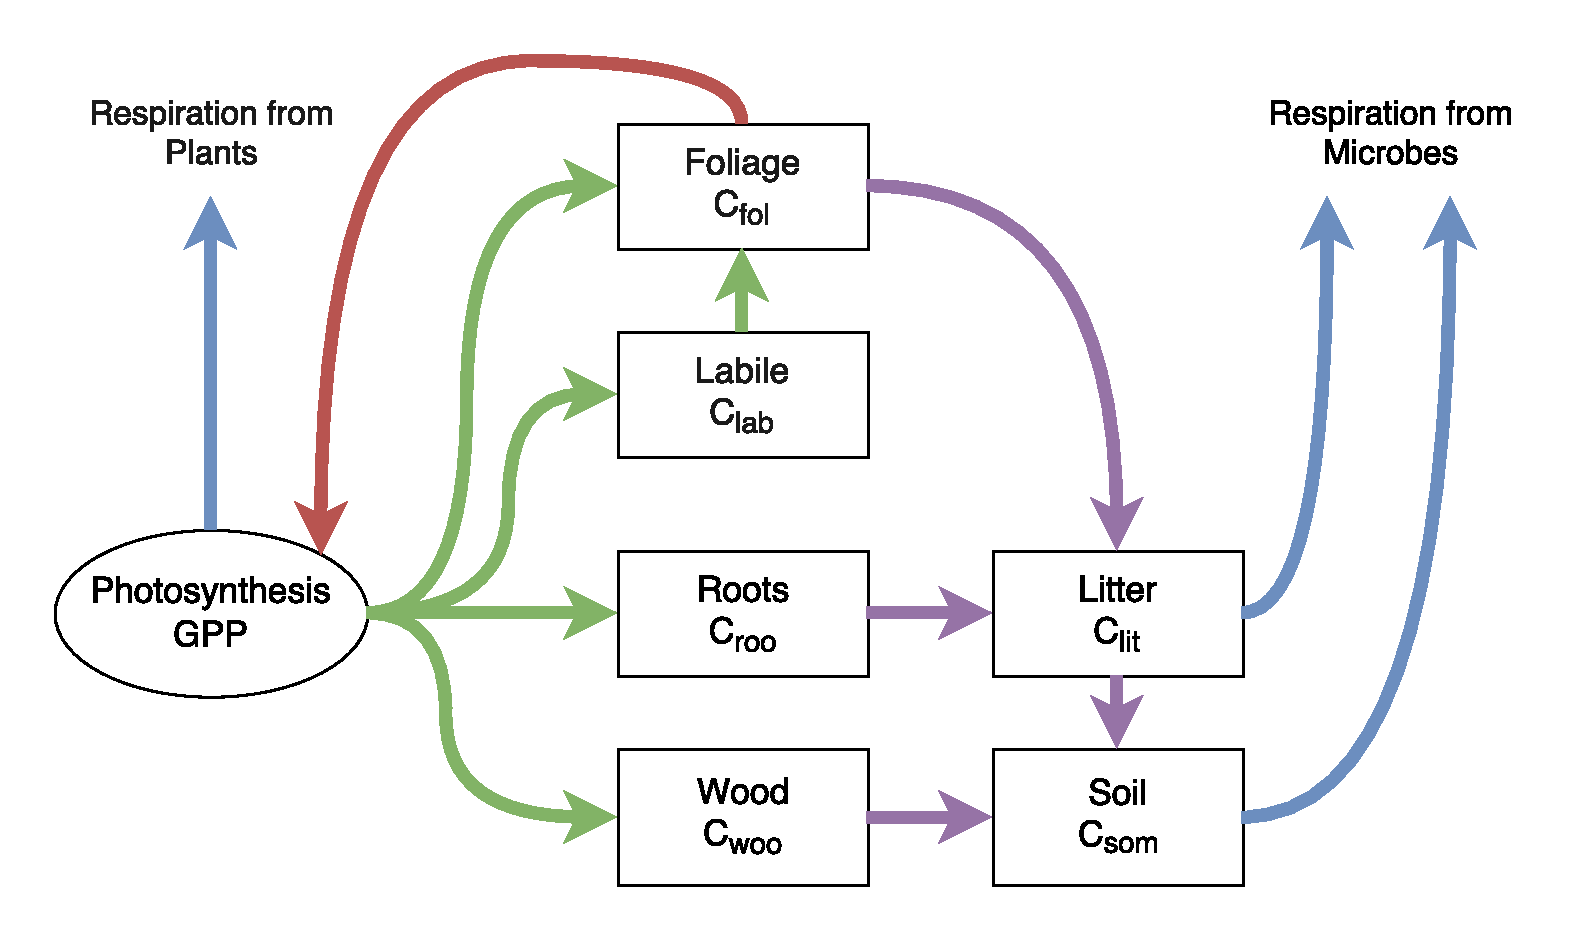
\includegraphics[width=0.5\textwidth]{chapter/chapter6/dalec2diag.pdf}
    \caption{Representation of the fluxes in the DALEC2 carbon balance model. Green arrows represent C allocation, purple arrows represent litter fall and decomposition fluxes, blue arrows represent respiration fluxes and the red arrow represents the influence of leaf area index in the $GPP$ function.} \label{fig:DALEC_mod}
\end{figure}

The model equations for the carbon pools at day $i$ are as follows:

\begin{align}
GPP^{i} &= ACM(C_{fol}^{i-1}, c_{lma}, c_{eff}, \Psi) \label{GPP}
\\C_{lab}^{i}&=C_{lab}^{i-1}+(1-f_{auto})(1-f_{fol})f_{lab}GPP^{i}-\Phi _{on}C_{lab}^{i-1}, \label{daleclab}
\\C_{fol}^{i}&=C_{fol}^{i-1}+\Phi_{on}C_{lab}^{i-1}+(1-f_{auto})f_{fol}GPP^{i}-\Phi_{off}C_{fol}^{i-1}, \label{dalec1}
\\C_{roo}^{i}&=C_{roo}^{i-1}+(1-f_{auto})(1-f_{fol})(1-f_{lab})f_{roo}GPP^{i}-\theta_{roo}C_{roo}^{i-1}, 
\\C_{woo}^{i}&=C_{woo}^{i-1}+(1-f_{auto})(1-f_{fol})(1-f_{lab})(1-f_{roo})GPP^{i}-\theta_{woo}C_{woo}^{i-1}, 
\\C_{lit}^{i}&=C_{lit}^{i-1}+\theta_{roo}C_{roo}^{i-1}+\Phi_{off}C_{fol}^{i-1}-(\theta_{lit}+\theta_{min})e^{\Theta T^{i-1}}C_{lit}^{i-1}, 
\\C_{som}^{i}&=C_{som}^{i-1}+\theta_{woo}C_{woo}^{i-1}+\theta_{min}e^{\Theta T^{i-1}}C_{lit}^{i-1}-\theta_{som}e^{\Theta T^{i-1}}C_{som}^{i-1}, \label{dalec5}
\end{align}
where $T^{i-1}$ is the daily mean temperature, $\Psi$ represents the meteorological driving data used in the $GPP$ function and $\Phi_{on} / \Phi_{off}$ are functions controlling leaf-on and leaf-off. Descriptions for each model parameter used in equations \eqref{GPP} to \eqref{dalec5} are included in the appendix in table~\ref{table:xbvars}. DALEC2 differs from the original DALEC in that it can be parameterised for both deciduous and evergreen sites with $\Phi_{on}$ and $\Phi_{off}$ being able to reproduce the phenology of either type of site. The full details of this version of DALEC can be found in \cite{Bloom2015}. 

\subsection{4D-Var} \label{4dvar}

Following the approach of \citet{Smith2011436} for joint state and parameter estimation, we consider the discrete nonlinear dynamical system given by
%
\begin{equation}
\textbf{z}_{i} = \textbf{f}_{i-1\rightarrow i}(\textbf{z}_{i-1}, \textbf{p}_{i-1}),
\end{equation}
where \( \textbf{z}_{i} \in \mathbb{R}^{n} \) is the state vector at time \( t_i \), \(\textbf{f}_{i-1 \rightarrow i}\) is the nonlinear model operator propagating the state at time \(t_{i-1}\) to time \(t_{i}\) for \(i = 1, 2, \dots, N\) and \(\textbf{p}_{i-1} \in \mathbb{R}^{q}\) is a vector of \(q\) model parameters at time \(t_{i-1}\). For DALEC2 the state vector \(\textbf{z}_{i}=(C_{lab}^{i}, C_{for}^{i}, C_{roo}^{i}, C_{woo}^{i}, C_{lit}^{i}, C_{som}^{i})^{T}\), with the parameters shown in table~\ref{table:xbvars}. Given a set of fixed parameters, the value of the forecast at time \(t_i\) is uniquely determined by the initial value. The model parameters are not updated by the nonlinear model operator, therefore the evolution of the parameters is given by,
%
\begin{equation}
\textbf{p}_{i} = \textbf{p}_{i-1}, 
\end{equation}
for $i= 1, 2, \dots, N$. We define the new vector $\textbf{x}$ by joining the parameter vector $\textbf{p}$ with the model state vector $\textbf{z}$, giving us the augmented state vector
\begin{equation}
\textbf{x} =
\begin{pmatrix}
\textbf{p} \\
\textbf{z}
\end{pmatrix}
\in \mathbb{R}^{q+n}.
\end{equation}
We define the augmented system model by
\begin{equation}
\textbf{x}_{i} = \textbf{m}_{i-1 \rightarrow i}(\textbf{x}_{i-1}), \label{eqn:nonlinmod}
\end{equation}
where
\begin{equation}
\textbf{m}_{i-1\rightarrow i}(\textbf{x}_{i-1}) =
\begin{pmatrix}
\textbf{p}_{i-1} \\
\textbf{f}_{i-1\rightarrow i}(\textbf{z}_{i-1}, \textbf{p}_{i-1})
\end{pmatrix}
=
\begin{pmatrix}
\textbf{p}_{i} \\
\textbf{z}_{i}
\end{pmatrix}
\in \mathbb{R}^{q+n}.
\end{equation}
The available observations at time $t_{i}$ are represented by the vector $\textbf{y}_{i} \in \mathbb{R}^{r_{i}}$ which are related to the augmented state vector through the equation
\begin{equation}
\textbf{y}_{i}=\textbf{h}_{i}(\textbf{x}_{i})+ \mathbf{ \epsilon}_{i},
\end{equation} 
where $\textbf{h}_{i}: \mathbb{R}^{q+n} \rightarrow \mathbb{R}^{r_{i}}$ is the observation operator mapping the augmented state vector to observation space and $\mathbf{\epsilon}_{i} \in \mathbb{R}^{r_{i}}$ represents the observation errors. These errors are usually assumed to be unbiased, Gaussian and serially uncorrelated with known covariance matrices $\textbf{R}_{i}$.

In the 4D-Var data assimilation detailed here we aim to find the parameter and initial state values such that the model trajectory best fits the data over some time window, given some prior information about the system. The output from 4D-Var is an updated set of parameters, and an updated model state, valid at the beginning of the time window. The updated model state may be used as initial conditions for a forecast using the full nonlinear DALEC2 model. We assume that at time $t_{0}$ we have an initial estimate to the augmented state, usually referred to as the background vector denoted $\textbf{x}^{b}$. This background is assumed to have unbiased, Gaussian errors with known covariance matrix $\textbf{B}$. Adding the background term ensures that our problem is well posed and that we can find a locally unique solution \citep{Tremolet2006}. In 4D-Var we aim to find the initial state that minimises the weighted least squares distance to the background while minimising the weighted least squares distance of the model trajectory to the observations over the time window $t_{0}, \dots, t_{N}$ \citep{lawless2013}. We do this by finding the state $\textbf{x}^{a}_{0}$ at time $t_{0}$ that minimises the cost function
\begin{equation}
J(\textbf{x}_0) = \frac{1}{2}(\textbf{x}_0-\textbf{x}^b)^{T}\textbf{B}^{-1}(\textbf{x}_0-\textbf{x}^b)+\frac{1}{2}\sum_{i=0}^{N}(\textbf{y}_i-\textbf{h}_i(\textbf{x}_i))^{T}\textbf{R}_{i}^{-1}(\textbf{y}_i-\textbf{h}_i(\textbf{x}_i)),
\end{equation}
subject to the augmented states $\textbf{x}_{i}$ satisfying the nonlinear dynamical model \eqref{eqn:nonlinmod}. The state that minimises the cost function, $\textbf{x}^{a}_{0}$, is commonly called the analysis. This state is found using a minimisation routine that takes as its input arguments the cost function, the background vector ($\textbf{x}^{b}$) and also the gradient of the cost function given as,
\begin{equation}
\nabla J(\textbf{x}_0) = \textbf{B}^{-1}(\textbf{x}_0-\textbf{x}^{b})-\sum_{i=0}^{N}\textbf{M}_{i,0}^{T}\textbf{H}_i^{T}\textbf{R}_{i}^{-1}(\textbf{y}_i-\textbf{h}_i(\textbf{x}_i))
\end{equation}
where $\textbf{H}_i = \frac{\partial \textbf{h}_i(\textbf{x}_i)}{\partial\textbf{x}_i}$ is the linearized observation operator and $\mathbf{M}_{i,0}=\mathbf{M}_{i-1}\mathbf{M}_{i-2}\cdots\mathbf{M}_0$ is the tangent linear model with $\mathbf{M}_i=\frac{\partial \textbf{m}_{i-1\rightarrow i}(\textbf{x}_{i})}{\partial \textbf{x}_{i}}$. In practice $\nabla J(\textbf{x}_0)$ is calculated using the method of Lagrange multipliers as shown in \citet{lawless2013}. We can rewrite the cost function and its gradient to avoid the sum notation as,
\begin{equation}
J(\textbf{x}_0) = \frac{1}{2}(\textbf{x}_0-\textbf{x}^b)^{T}\textbf{B}^{-1}(\textbf{x}_0-\textbf{x}^b)+\frac{1}{2}(\hat{\textbf{y}}-\hat{\textbf{h}}(\textbf{x}_0))^{T}\hat{\textbf{R}}^{-1}(\hat{\textbf{y}}-\hat{\textbf{h}}(\textbf{x}_0)) \label{costfn}
\end{equation}
and
\begin{equation}
\nabla J(\textbf{x}_0) = \textbf{B}^{-1}(\textbf{x}_0-\textbf{x}^b)-\hat{\mathbf{H}}^{T}\hat{\textbf{R}}^{-1}(\hat{\textbf{y}}-\hat{\textbf{h}}(\textbf{x}_0)), \label{gradcostfn}
\end{equation}
where,
\begin{equation}
\hat{\textbf{y}}=
\begin{pmatrix}
\textbf{y}_0 \\
\textbf{y}_1\\
\vdots \\
\textbf{y}_N
\end{pmatrix},
\hspace{1mm}
\hat{\textbf{h}}(\textbf{x}_0)=
\begin{pmatrix}
\textbf{h}_0(\textbf{x}_0) \\
\textbf{h}_1(\textbf{m}_{0\rightarrow 1}(\mathbf{x}_{0}))\\
\vdots \\
\textbf{h}_N(\textbf{m}_{0\rightarrow N}(\mathbf{x}_{0}))
\end{pmatrix},
\hspace{1mm}
\hat{\mathbf{R}}=
\begin{pmatrix}
\mathbf{R}_{0, 0} & \mathbf{R}_{0, 1} & \dots & \mathbf{R}_{0, N} \\
\mathbf{R}_{1, 0} & \mathbf{R}_{1, 1} & \dots & \mathbf{R}_{1, N} \\
\vdots & \vdots & \ddots & \vdots \\
\mathbf{R}_{N, 0} & \mathbf{R}_{N, 1} & \dots & \mathbf{R}_{N, N}
\end{pmatrix}
\hspace{1mm} \text{and} \hspace{3mm}
\hat{\mathbf{H}}=
\begin{pmatrix}
\mathbf{H}_0 \\
\mathbf{H}_1\mathbf{M}_0\\
\vdots \\
\mathbf{H}_N\mathbf{M}_{N,0}
\end{pmatrix}.
\end{equation}

Solving the cost function in this form also allows us to build serial time correlations into the observation error covariance matrix $\hat{\mathbf{R}}$. The off-diagonal blocks of $\hat{\mathbf{R}}$ represent correlations in time between assimilated observations and are usually taken to be zero. In section~\ref{sec:corR} we show how these off-diagonal blocks can be specified. We can also calculate the posterior or analysis error covariance matrix after assimilation as,
\begin{equation}
\mathbf{A} = (\textbf{B}^{-1} + \hat{\mathbf{H}}^{T}\hat{\textbf{R}}^{-1}\hat{\mathbf{H}})^{-1}. \label{eqn:Amat}
\end{equation}
We can use this matrix to estimate the uncertainty in our parameter and initial state variables after assimilation.
%Forecast skill score, $SS = 1 - \frac{MSE_{forecast}}{MSE_{ref}}$, http://en.wikipedia.org/wiki/Forecast_skill

\subsection{Implementation and testing of 4D-Var system} \label{sec:implement4dvar}

In our DALEC2 4D-Var scheme we are performing joint parameter and state estimation. Typically MCMC techniques have been used for joint parameter and state estimation with functional ecology models, such as DALEC2. However 4D-Var has been used for joint parameter and state estimation with global carbon cycle models \citep{Kaminski2013}. The variational approach is computationally efficient and robust, making it particularly suited to large problems with complex models. The augmented state vector, $\textbf{x}_0$, corresponds to the vector of the 17 model parameters and 6 initial carbon pool values, which can be found in the appendix in table~\ref{table:xbvars}. Here the nonlinear model (DALEC2) only updates the initial carbon pool values when evolving the augmented state vector forward in time with the parameters being held constant. To find the background estimate, $\textbf{x}^{b}$, to the augmented state vector we can either use a previous DALEC2 model forecast estimate of the state of the system for the site (when available) or use expert elicitation to define likely state and parameter values and ranges for the site. The background vector $(\textbf{x}^b)$ and its corresponding standard deviations (see table~\ref{table:xbvars}) used in this paper were provided from existing runs of the the CARbon DAta-MOdel fraMework (CARDAMOM) \citep{Exbrayat2015}. The CARDAMOM output is a dataset derived from satellite observations of leaf area index which provides a reasonable first guess to DALEC2 state and parameter values for the Alice Holt research site. In this paper we assimilate observations of daily NEE. From \citet{Richardson200838} the measurement error in observations of daily NEE is between $0.2$ to $0.8~\text{gCm}^{-2}\text{day}^{-1}$.  \citet{Richardson200838} also shows that flux errors are heteroscedastic. We assume a constant standard deviation of $0.5~\text{gCm}^{-2}\text{day}^{-1}$ in the assimilated observations of daily NEE as we found this standard deviation gave the best weighting to the observations in the assimilation algorithm, producing the best results for the forecast of NEE after assimilation. Assuming this constant standard deviation also allows for correlations in time between observation errors to be included more easily. Ignoring the heteroscedastic nature of NEE errors may influence results by giving observations of larger magnitude a higher weight than would be realistic. Future work should try to incorporate the heteroscedastic nature of NEE errors.

In order to find the tangent linear model (TLM) for DALEC2 it is necessary to find the derivative of the model at each time step with respect to the 17 model parameters and the 6 carbon pools. We use the AlgoPy automatic differentiation package \citep{Walter2013} in Python to calculate the TLM at each time step. This package uses forward mode automatic differentiation to calculate the derivative of the model. In the following tests we use a diagonal approximation to the background and observation error covariance matrices so that, 
$\textbf{B}_{diag}=\text{diag}(\bm{\sigma}_b)^2$ and $\hat{\textbf{R}}_{diag}=\text{diag}(\bm{\sigma}_o )^2$,
where $\bm{\sigma}_b$ is the vector of background standard deviations found in table~\ref{table:xbvars} and $\bm{\sigma}_o$ is the vector of observational standard deviations, for a single observation of NEE $\sigma_o=0.5~\text{gCm}^{-2}\text{day}^{-1}$. To minimise the cost function we use the truncated Newton iteration method \citep{Nocedal1999} from the Python package Scipy.optimize \citep{scipy2015}. This method uses a number of stopping criteria to ensure convergence to a minimum of our cost function. In sections \ref{sec:testtlm} to \ref{sec:testgrad} we show tests of our scheme. 


\subsubsection{Test of tangent linear model} \label{sec:testtlm}

The TLM is used in the calculation of the gradient of our cost function in 4D-Var. We can have confidence that our implementation of the TLM for DALEC2 is correct as it passes the following relevant tests \citep{Li1994}. In 4D-Var we assume the tangent linear hypothesis,
\begin{equation}
\textbf{m}_{0\rightarrow i}(\mathbf{x}_0+\gamma \delta\mathbf{x}_0) \approx \textbf{m}_{0 \rightarrow i}(\mathbf{x}_0) +\gamma \mathbf{M}_{i,0} \delta\mathbf{x}_0, \label{TLH}
\end{equation}
where $\delta\mathbf{x}_0$ is a perturbation of the initial augmented state $\textbf{x}_{0}$ and $\gamma$ is a parameter controlling the size of this perturbation. The validity of this assumption depends on how nonlinear the model is, the length of the assimilation window and the size of the augmented state perturbation $\delta\mathbf{x}_0$. We can test this by rearranging equation~\eqref{TLH} to find,
\begin{equation}
\frac{||\textbf{m}_{0\rightarrow i}(\mathbf{x}_0+\gamma \delta\mathbf{x}_0) - \textbf{m}_{0 \rightarrow i}(\mathbf{x}_0)-\gamma\mathbf{M}_{i,0}\delta\mathbf{x}_0||}{||\gamma\mathbf{M}_{i,0}\delta\mathbf{x}_0||} \rightarrow 0, \label{tlmtest}
\end{equation}
as $\gamma \rightarrow 0$ (here we are using the Euclidean norm). Equation~\eqref{tlmtest} should hold if our implementation of the TLM is correct, even for a weakly non-linear model. Figure~\ref{fig:tlm} shows equation~\eqref{tlmtest} plotted for DALEC2 with $i$ fixed at 731 days, a fixed $5\%$ perturbation $\delta\mathbf{x}_0$ and values of $\gamma$ approaching zero . Figure~\ref{fig:tlm} shows that the TLM behaves as expected for values of $\gamma$ approaching $0$. This was also tested for different choices of $\textbf{x}_{0}$ and sizes of perturbation with similar results.


\begin{figure}[ht]
    \centering
    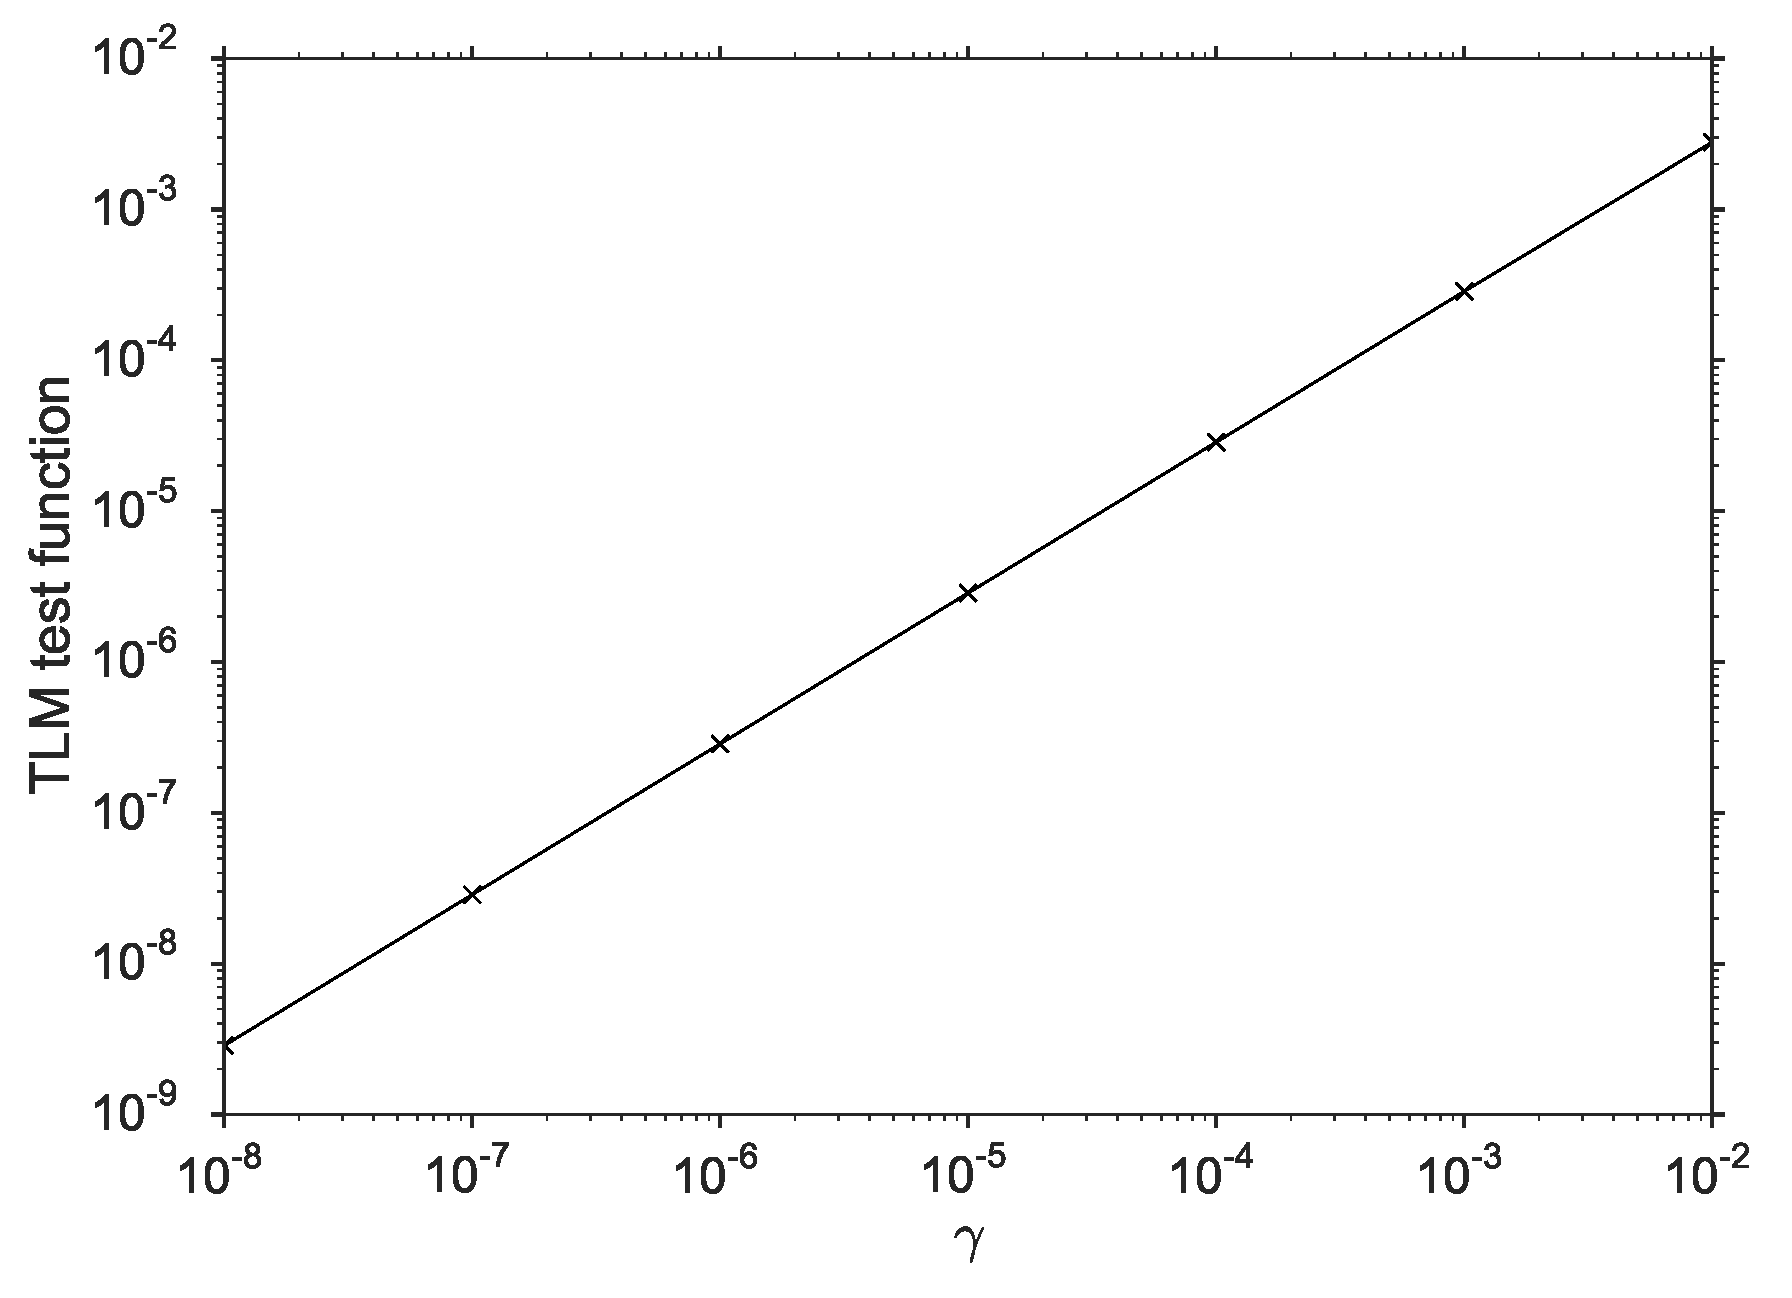
\includegraphics[width=0.5\textwidth]{chapter/chapter6/linmoderr.eps}
    \caption{Plot of the tangent linear model test function (equation \eqref{tlmtest}) for DALEC2, for a fixed TLM evolving the perturbed augmented state 731 days forward in time and a fixed $5\%$ perturbation, $\delta \textbf{x}_0$.}
    \label{fig:tlm}
\end{figure}

It is also useful to show how the TLM behaves over a time window to see how the error in the TLM grows as we evolve the augmented state further forward in time. We again rearrange equation \eqref{TLH} with an additional error term to find, 
\begin{equation}
\text{percentage error in TLM} =  \frac{||m_{0\rightarrow i}(\mathbf{x}_0+\gamma \delta\mathbf{x}_0) - m_{0 \rightarrow i}(\mathbf{x}_0) - \gamma\mathbf{M}_{i,0}  \delta\mathbf{x}_0||}{|| \gamma\mathbf{M}_{i,0}  \delta\mathbf{x}_0||} \times 100. \label{pertlmtest}
\end{equation}

\begin{figure}[ht]
    \centering
    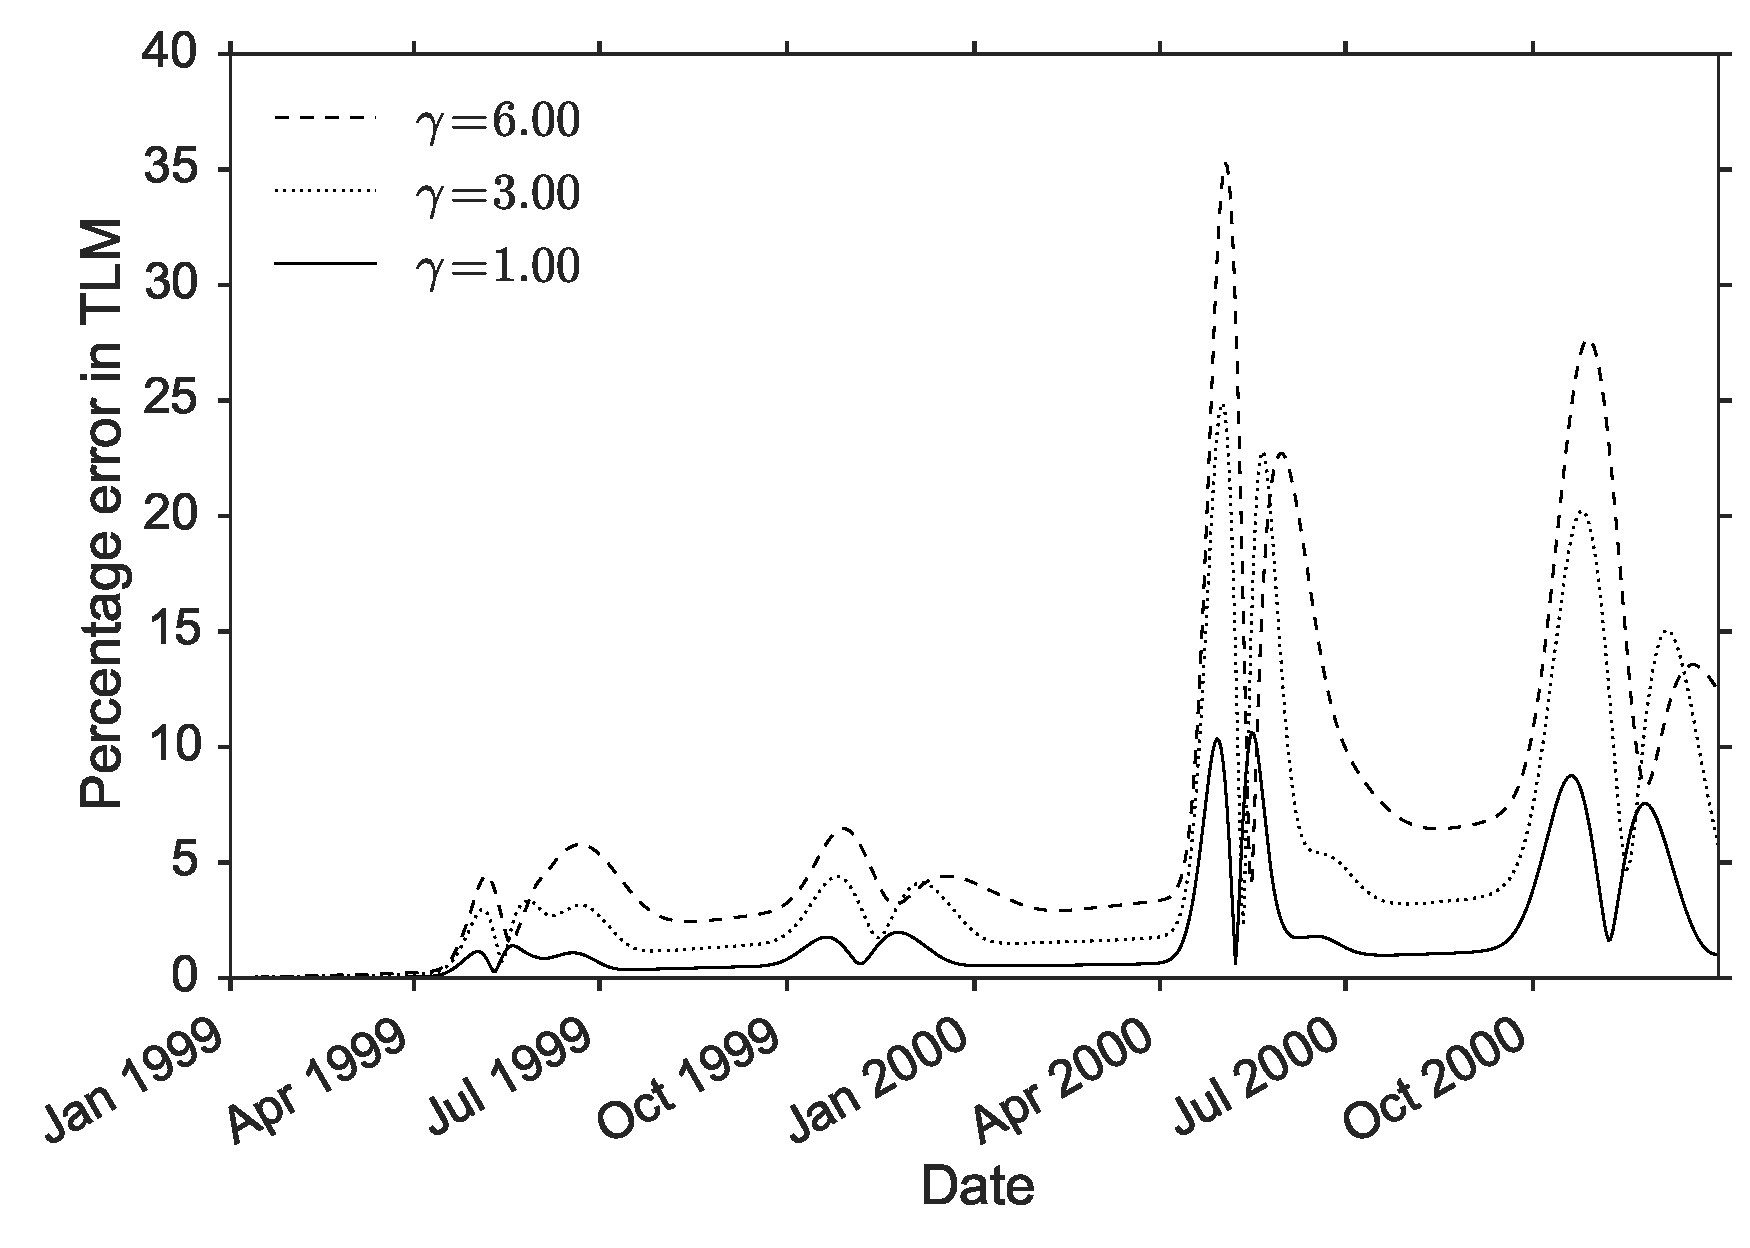
\includegraphics[width=0.5\textwidth]{chapter/chapter6/percenterrlinmod.eps}
    \caption{Plot of the percentage error in the tangent linear model (equation \eqref{pertlmtest}) for DALEC2 when evolving the model state forward over a period of two years with three different values of $\gamma$ and a fixed $5\%$ perturbation $\delta \textbf{x}_0$.}
    \label{fig:tlm_error}
\end{figure}

In figure \ref{fig:tlm_error} we plot the percentage error in the TLM tested throughout a two-year period as DALEC2 is run forward. From figure \ref{fig:tlm_error} we can see that the TLM for DALEC2 performs well after being run forward a year with less than a $7\%$ error for all values of $\gamma$. By the second year we see some peaks in the error in spring and autumn. This is due to leaf on and leaf off functions in the TLM going out of phase with the nonlinear DALEC2. At these peaks the error reaches a maximum at $35\%$ then coming back to around $10\%$ before growing again in the autumn. Although this level of error is still acceptable we present results using a one year assimilation window in this paper as in practice we could cycle assimilation windows to make use of multiple years of data \citep{moodycycled4dvar}.

\subsubsection{Test of adjoint model} 

The adjoint model we have implemented for DALEC2 passes correctness tests. For the TLM $\mathbf{M}_{i,0}$ and its adjoint $\mathbf{M}_{i,0}^{T}$ we have the identity
\begin{equation}
<\mathbf{M}_{i,0}\delta\textbf{x}_0, \mathbf{M}_{i,0}\delta\textbf{x}_0> = <\delta\textbf{x}_0, \mathbf{M}_{i,0}^{T}\mathbf{M}_{i,0}\delta\textbf{x}_0> \label{eqn:adjoint_test}
\end{equation}
for any inner product $<, >$ and perturbation $\delta \textbf{x}_0$. This is derived from the adjoint identity \citep{lawless2013}. Using the Euclidean inner product, equation~\eqref{eqn:adjoint_test} is equivalent to
\begin{equation}
(\mathbf{M}_{i,0}\delta\textbf{x}_0)^{T} (\mathbf{M}_{i,0}\delta\textbf{x}_0) = \delta\textbf{x}_0^{T} (\mathbf{M}_{i,0}^{T}(\mathbf{M}_{i,0}\delta\textbf{x}_0)).
\end{equation}
We evaluated the left hand side and right hand side of this identity for differing values of $\textbf{x}_0$ and size of perturbation $\delta \textbf{x}_0$ and showed that they were equal to machine precision.

\subsubsection{Gradient test} \label{sec:testgrad}

The 4D-Var system we have developed passes tests for the gradient of the cost function \citep{Navon1992}. In the implementation of the cost function and its gradient we regularise the problem using a variable transform \citep{Freitag2010}. For the cost function $J$ and its gradient $\nabla J$ we can show that we have implemented $\nabla J$ correctly using the identity,
\begin{equation}
f(\alpha)=\frac{| J( \textbf{x}_0 + \alpha \textbf{b}) - J(\textbf{x}_0) |}{\alpha \textbf{b}^{T} \nabla J(\textbf{x}_0)} = 1 + O(\alpha),
\end{equation}
where $\textbf{b}$ is a vector of unit length and $\alpha$ is a parameter controlling the size of the perturbation. For small values of $\alpha$ not too close to machine precision we should have $f(\alpha)$ close to 1. Figure~\ref{fig:costone} shows $f(\alpha)$ for a 365 day assimilation window with $\textbf{b}=\textbf{x}_0||\textbf{x}_0||^{-1}$, we can see that $f(\alpha) \rightarrow 1$ as $\alpha \rightarrow 0$, as expected until $f(\alpha)$ gets too close to machine zero at order $\alpha = 10^{-11}$. This was also tested with $\textbf{b}$ in different directions and similar results obtained.

We can also plot $|f(\alpha)-1|$, where we expect $|f(\alpha)-1| \rightarrow 0$ as $\alpha \rightarrow 0$.  In figure~\ref{fig:cost} we have plotted $|f(\alpha)-1|$ for the same conditions as in figure~\ref{fig:costone}, we can see that $|f(\alpha) - 1| \rightarrow 0$ as $\alpha \rightarrow 0$, as expected. This gives us confidence that the gradient of the cost function is implemented correctly.
%$\nabla J(\textbf{x}_0)||\nabla J(\textbf{x}_0)||^{-1}$. 

\begin{figure}[ht]
    \centering
    \begin{subfigure}[b]{0.49\textwidth}
        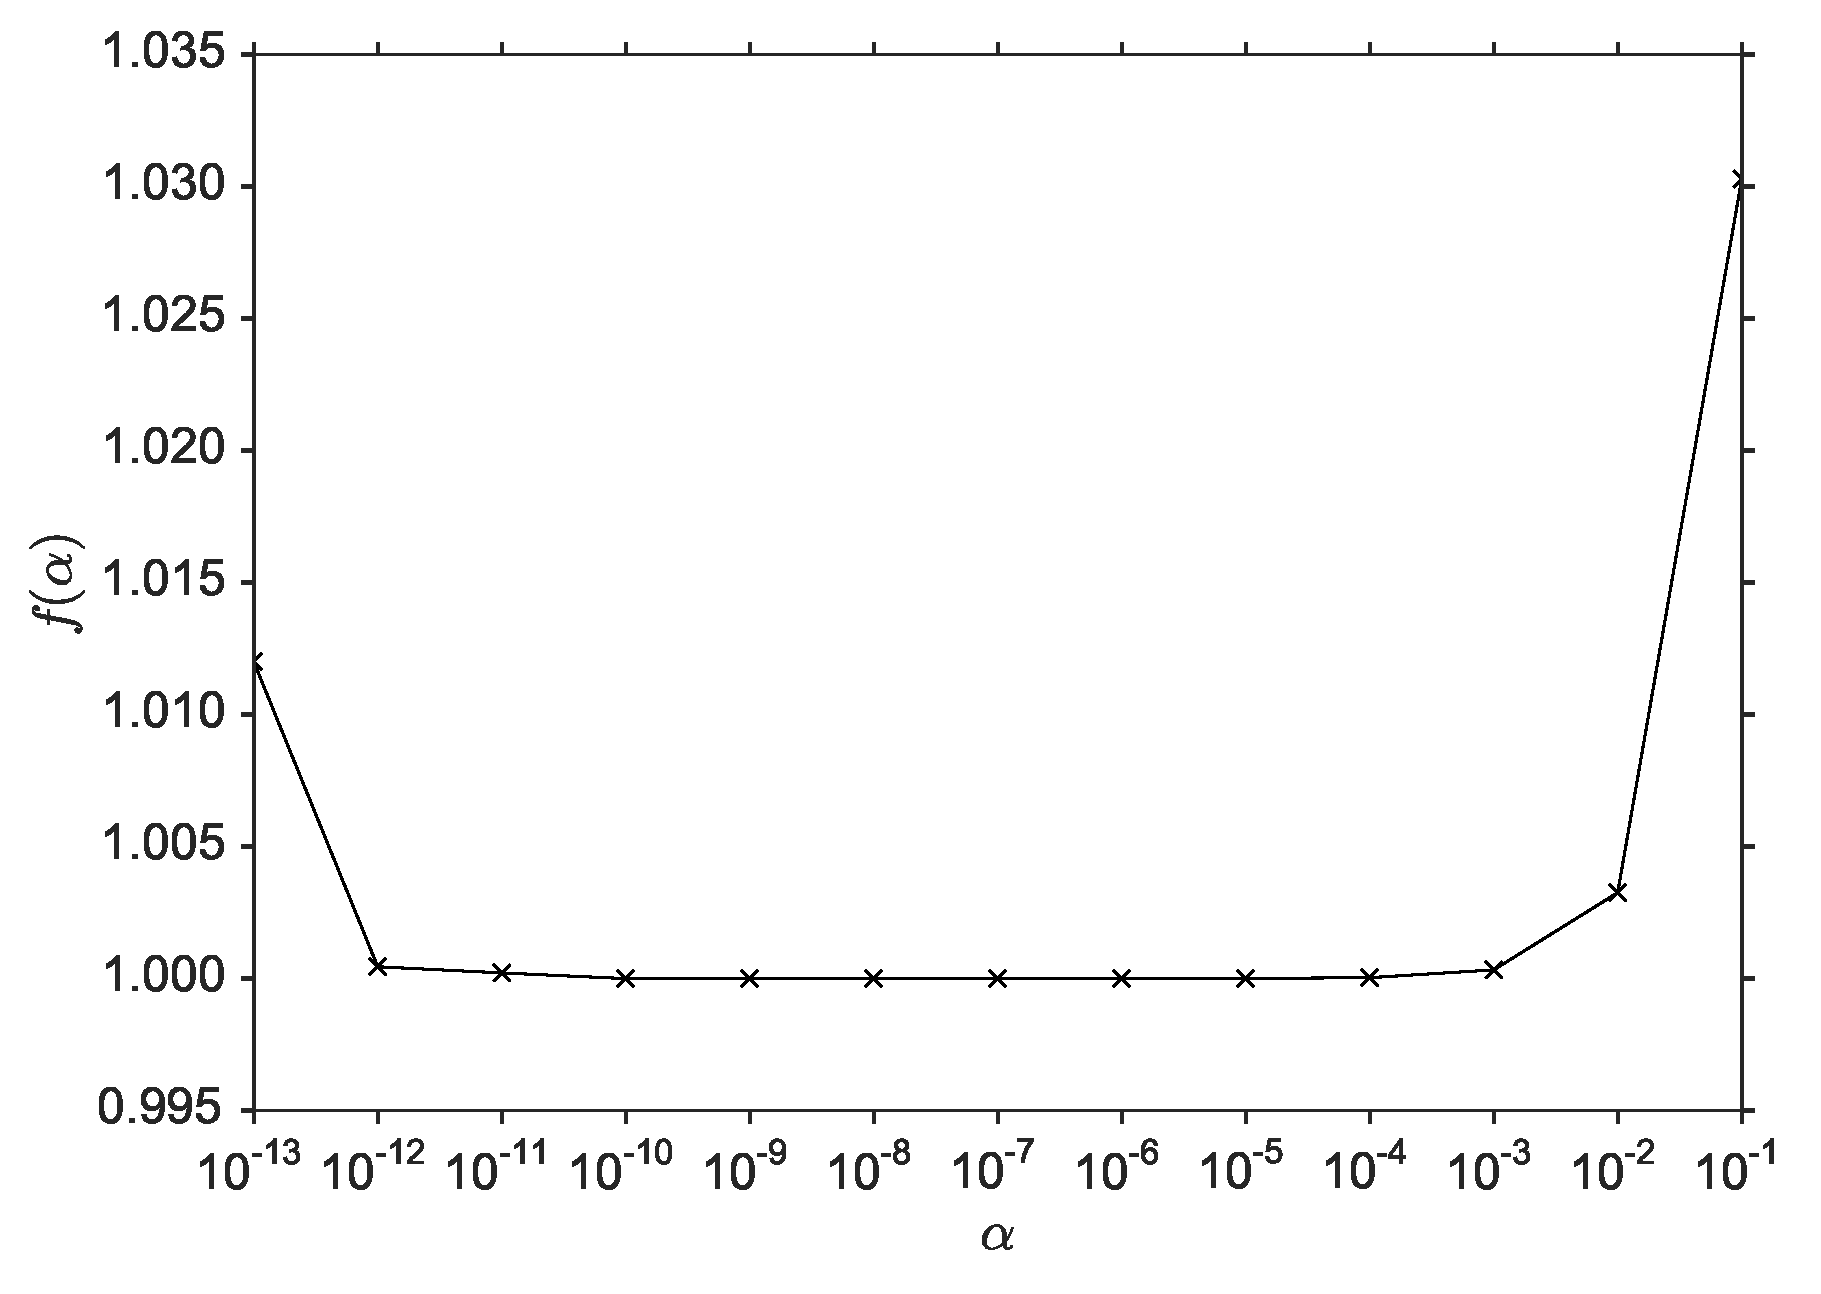
\includegraphics[width=\textwidth]{chapter/chapter6/costone_cvt.eps}
        \caption{$f(\alpha)$ test}
        \label{fig:costone}
    \end{subfigure}
    \begin{subfigure}[b]{0.49\textwidth}
        \includegraphics[width=\textwidth]{chapter/chapter6/cost_cvt.eps}
        \caption{$|f(\alpha) - 1|$ test}
        \label{fig:cost}
    \end{subfigure}
    \caption{Tests of the gradient of the cost function for a 365 day assimilation window with $\textbf{b}=\textbf{x}_0||\textbf{x}_0||^{-1}$.}
    \label{fig:testgradcostone}
\end{figure}

\subsection{Including correlations in the background error covariance matrix} \label{sec:corB}

As discussed in section~\ref{sec:intro}, including correlations in \textbf{B} impacts how information from assimilated observations is spread between different types of analysis variables \citep{bannister2008review}. We explored a number of different methods in order to include parameter-state correlations in \textbf{B}. In this paper we present a method using a set of ecological dynamical constraints, based on expert judgement, on model parameters and state variables from \citet{Bloom2015}. \citet{Bloom2015} show that implementing these constraints in a Metropolis Hastings MCMC data assimilation routine improves results significantly. The constraints impose conditions on carbon pool turnover and allocation ratios, steady state proximity and growth and the decay of model carbon pools.

In order to create a correlated background error covariance matrix, $\textbf{B}_{corr}$, using these constraints we create an ensemble of state vectors which we then take the covariance of to give us $\textbf{B}_{corr}$. To create this ensemble we use the following procedure:
\begin{enumerate}
\item Draw a random augmented state vector, $\textbf{x}_i$, from the multivariate truncated normal distribution described by
\begin{equation}
\textbf{x}_i \sim \mathcal{N}(\textbf{x}^b, \textbf{B}_{diag}),
\end{equation} 
where $\textbf{B}_{diag}$ is the diagonal matrix described in section~\ref{sec:implement4dvar} and $\textbf{x}_i$ is bound by the parameter and state ranges given in table~\ref{table:xbvars} in the appendix.
\item Test this $\textbf{x}_i$ with the ecological dynamical constraints (requiring us to run the DALEC2 model using this state).
\item If $\textbf{x}_i$ passes it is added to our ensemble, else it is discarded.
\end{enumerate}
Once we have a full ensemble we then take the covariance of the ensemble to find $\textbf{B}_{corr}$. We chose an ensemble size of 1500 as a qualitative assessment using a larger ensemble showed little difference in correlations. In figure \ref{fig:Bcorr} we have plotted the correlation matrix or normalised error covariance matrix associated with $\textbf{B}_{corr}$. This matrix includes both positive and negative correlations between parameter and state variables, with correlations of 1 down the diagonal between variables of the same quantity as expected. The largest positive off-diagonal correlation is $0.42$ between $f_{lab}$ and $C_{lab}$. This makes physical sense as $f_{lab}$ is the parameter controlling the amount of GPP allocated to the labile carbon pool, $C_{lab}$.

\begin{figure}[ht]
    \centering
    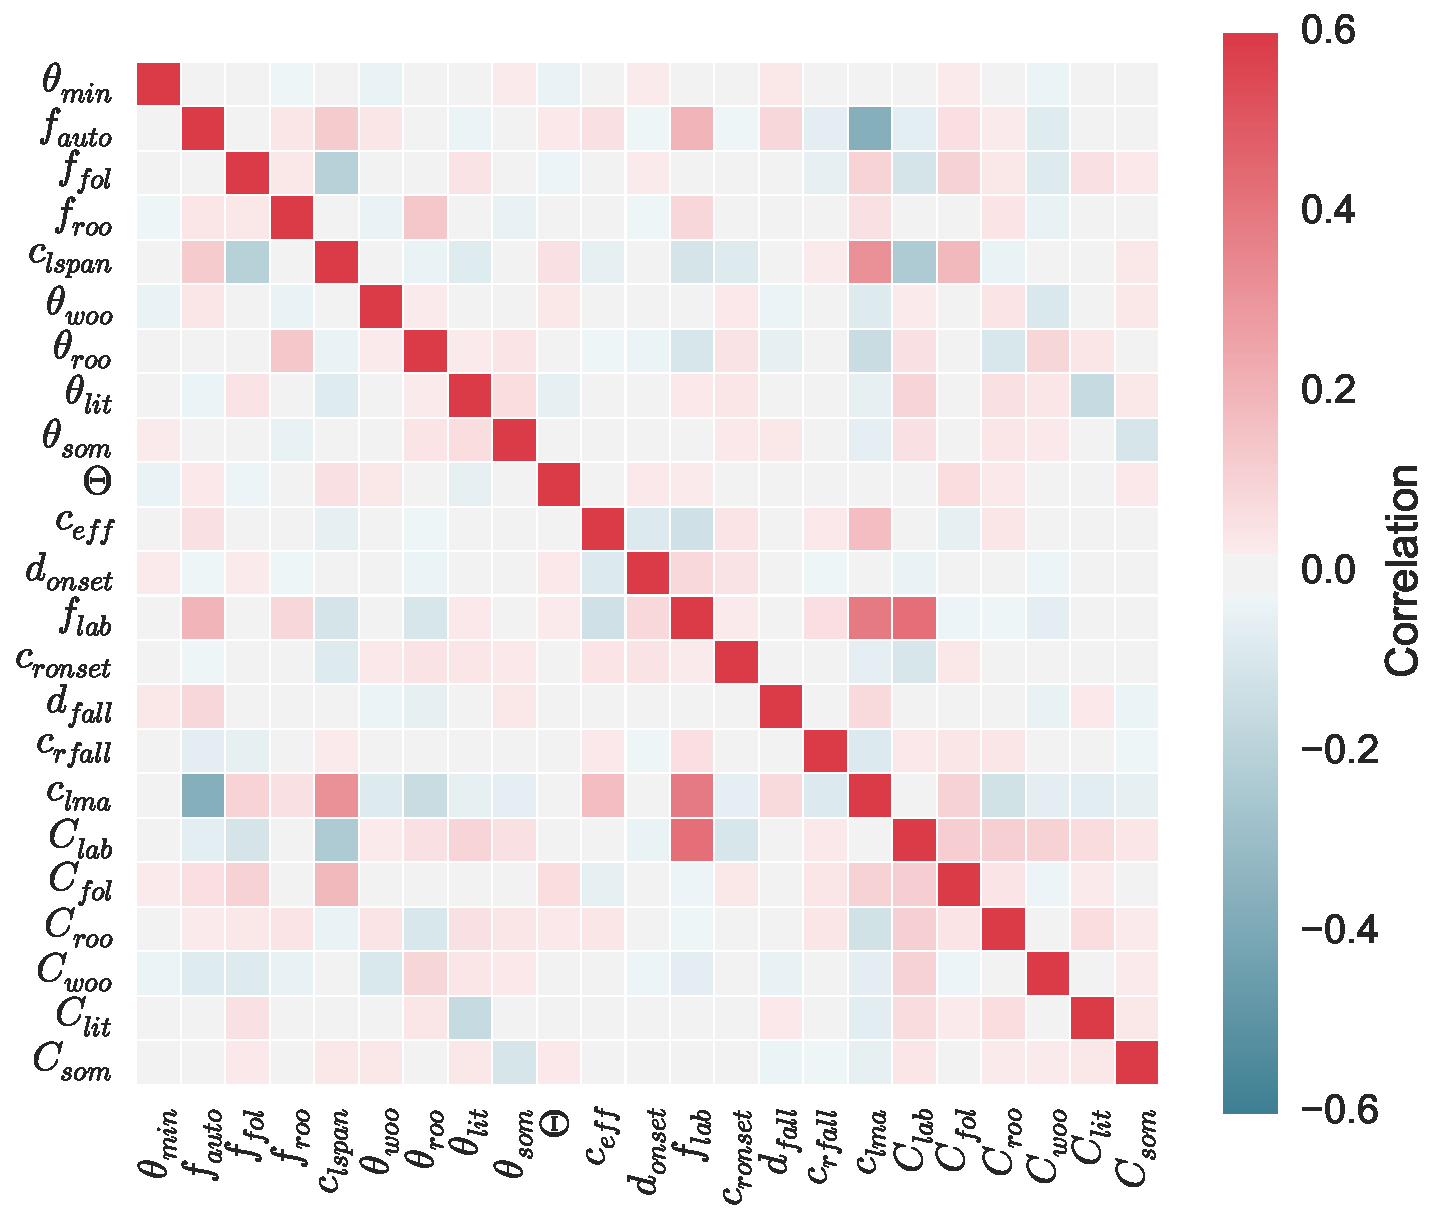
\includegraphics[width=0.55\textwidth]{chapter/chapter6/bedccor2.pdf}
    \caption{Background error correlation matrix created using method in section \ref{sec:corB}. Here the correlation scale for off-diagonal values ranges from $-0.5$ to $0.5$ with the correlation along the diagonal being $1$. For explanation of parameter and state variable symbols see table~\ref{table:xbvars}.}
    \label{fig:Bcorr}
\end{figure}

\subsection{Specifying serial correlations in the observation error covariance matrix} \label{sec:corR}

The observation error covariance matrix does not only represent the instrumentation error for an observation but also the error in the observation operator (mapping the model state to the observation) and representativity error (error arising from the model being unable resolve the spatial and temporal scales of the observations). These other sources of error represented in $\hat{\textbf{R}}$ can also lead to correlations between observation errors \citep{Waller2014}. Errors in NEE observations come from different sources such as instrument errors, sampled ecosystem structure from the variable footprint of the flux tower and turbulent conditions (when there is low turbulence and limited air mixing the magnitude of NEE is underestimated). These errors due to turbulence can still have effect even after $u^{*}$ filtering \citep{Papale2006}. Due to this dependence on atmospheric conditions we expect the errors in observations of NEE to be serially correlated, as the atmospheric signal itself is serially correlated \citep{Daley1992}. If we were assimilating half hourly observations of NEE we would expect stronger correlations between observation errors, as atmospheric conditions are more constant at this time scale, with correlations between observation errors getting weaker with lower frequency observations. Although some studies suggest that the correlation between NEE measurement errors on the scale of a day is negligible \citep{lasslop:hal-00297973}, it is also likely that error in the observation operator and representativity error will lead to observation error correlations for NEE \citep{Waller2014}.

In section~\ref{4dvar} we have re-written the 4D-Var cost function in equation~\eqref{costfn} in order to allow the specification of serial observation error correlations in our assimilation scheme. These serial correlations are represented by the off-diagonal blocks of $\hat{\mathbf{R}}$. In work carried out with spatial correlations it has been shown that the structure of the correlation is not critical and that it is better to include some estimate of error correlation structure in the observation error covariance matrix than wrongly assume that errors are independent \citep{Stewart2013, Healy2005}. As a first attempt we try including temporal correlations on the scale of the observation frequency. We adapt the simple Gaussian model found in \citet{jarvinen1999variational} (a second order autoregressive correlation function was also tested but is not presented here). The correlation $r$ between 2 observations at times $t_1$ and $t_2$ is given as,
\begin{equation}
r =
\begin{cases} 
      a \text{exp} \bigg[ \frac{-(t_1 - t_2)^2}{\tau^2} \bigg] + (1- a)\delta_{t_1 - t_2} & |t_1 - t_2| \leq \eta \\
      0 & \eta < |t_1 - t_2| 
   \end{cases}
   , \label{eqn:corr_fn}
\end{equation}
where $\tau$ is the e-folding time in days, $a$ controls the strength of correlation, $\delta$ is the Kronecker delta and $\eta$ is the cut off time after which the correlation between two observation errors is zero. We have incorporated a cut off for correlations between observation errors as the assumed correlation length scale for the assimilated observations is short. This cut off along with the form of correlation function using the Kronecker delta helps ensure $\hat{\mathbf{R}}$ is positive definite and therefore invertible, as required in the assimilation process. The standard deviation assumed in the observations of NEE is $0.5~\text{gCm}^{-2}\text{day}^{-1}$ as described in section~\ref{sec:implement4dvar}.

\begin{figure}[ht]
    \centering
    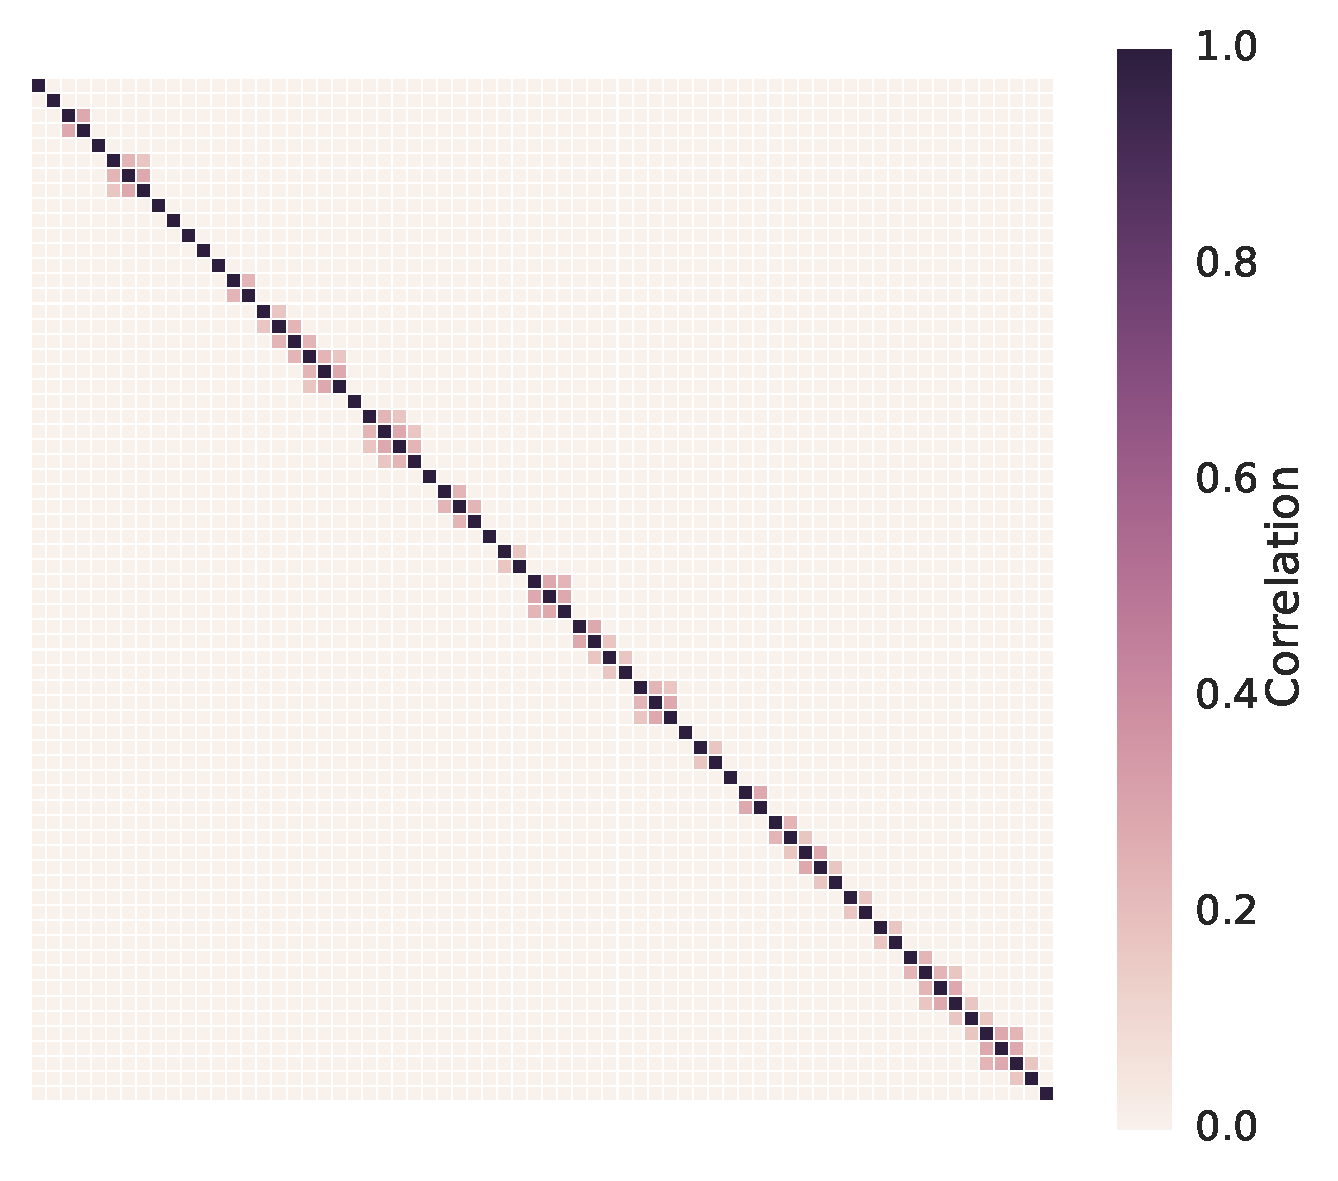
\includegraphics[width=0.5\textwidth]{chapter/chapter6/rcorcor.eps}
    \caption{Observation error correlation matrix for the 67 observations used in assimilation created using method in section \ref{sec:corR} with $\tau = 4$, $a=0.3$ and $\eta=4$.}
    \label{fig:Rcorr}
\end{figure}

Figure~\ref{fig:Rcorr} shows the correlation matrix for $\hat{\mathbf{R}}$ created using equation~\eqref{eqn:corr_fn}. Here observations made on adjacent days will have an error correlation of 0.3; this will then decay exponentially for observations farther apart in time. There are 67 NEE observations in this one year assimilation window. These observations are not all on adjacent days and this is evident in the structure of $\hat{\mathbf{R}}$. The effect of the short e-folding time chosen here ($\tau=4$) provides the desired structure. 

\section{Results} \label{sec:results}

\subsection{Experiments} \label{sec:exps}

In the following sections we present the results of four experiments where we vary the representations of $\textbf{B}$ and $\hat{\mathbf{R}}$ while assimilating the same NEE observations in the window from the beginning of January 1999 to the end of December 1999. As shown in figure~\ref{fig:tlm_error} the performance of the tangent linear model deteriorates after the first year. We then forecast the NEE over the next 14 years (Jan 2000 - Dec 2013) and compare with the observed data. Using this shorter analysis window with a long forecast allows us to see the effect of including correlations in the error statistics more clearly, as we have a longer time-series of data with which to judge our forecast after data assimilation. These experiments are outlined in table~\ref{table:exps_tab} where $\textbf{B}_{diag}$ and $\hat{\mathbf{R}}_{diag}$ are the diagonal matrices of the parameter and state variances and the observations variances respectively and $\textbf{B}_{corr}$ and $\hat{\mathbf{R}}_{corr}$ are the matrices as specified in section~\ref{sec:corB} and section~\ref{sec:corR} respectively.

\begin{table}[ht] 
\begin{center}
	\begin{tabular}{| l | l | l | l | l |}
	\hline
	Experiment & $\textbf{B}_{diag}$ & $\hat{\mathbf{R}}_{diag}$ & $\textbf{B}_{corr}$ &
	$\hat{\mathbf{R}}_{corr}$ \\ \hline
	A & $\times$ & $\times$ & & \\ \hline
	B & & $\times$ & $\times$ & \\ \hline
	C & $\times$ & & & $\times$ \\ \hline
	D & & & $\times$ & $\times$ \\ 
	\hline
	\end{tabular}
	\caption{The combination of error covariance matrices used in each data assimilation experiment.}
	\label{table:exps_tab}
\end{center} 
\end{table}

\subsection{Experiment A} \label{sec:expa}
In this experiment $\textbf{B}_{diag}$ and $\hat{\textbf{R}}_{diag}$ were used in the assimilation as described in section~\ref{sec:exps}. Because these contain no correlations this experiment forms the baseline by which the subsequent results from assimilation experiments are judged.  

Figure~\ref{fig:4dvardiagBR} shows assimilation and forecast results for NEE. We can see that assimilating the observations of NEE has improved the background with the analysis trajectory (green line) fitting well with the observations during the assimilation window (Jan 1999- Dec 1999). The analysis trajectory then diverges in the forecast (Jan 2000 - Dec 2013). This can be seen more clearly in figue~\ref{fig:broke4dvardiagBR}, where there is an over prediction of respiration in the winter and the seasonal cycle does not match that of the observations. This is also shown in figure~\ref{fig:Amoddat_resid} where we have plotted the model-data differences for a year's period averaged over the 14 years in the forecast period. Figure~\ref{fig:Amoddat_resid} shows that the largest errors in our posterior model forecast occur as a result of not capturing the phenology of the site correctly, in particular the start of the season from April to June.
 
To see how well the forecast performs after assimilation we show a scatter plot of modelled NEE against observed NEE in figure~\ref{fig:forecastscatBR}. From table~\ref{table:results} the predictions have a Root-Mean-Square Error (RMSE) of $4.22 ~\text{gCm}^{-2}\text{day}^{-1}$ and a bias of $-0.3 ~\text{gCm}^{-2}\text{day}^{-1}$ for the forecast of NEE, whereas the analysis (Jan 1999 - Dec 1999) has a RMSE of $1.36 ~\text{gCm}^{-2}\text{day}^{-1}$ and a bias of $-0.03 ~\text{gCm}^{-2}\text{day}^{-1}$. The background trajectory is the model trajectory for DALEC2 when run using the prior estimate of the parameter and initial state values described in section~\ref{sec:implement4dvar}. The background or prior model trajectory has a RMSE of $3.86 ~\text{gCm}^{-2}\text{day}^{-1}$ and a bias of $-1.60 ~\text{gCm}^{-2}\text{day}^{-1}$ in the analysis window (Jan 1999 - Dec 1999) and the same RMSE of $3.86 ~\text{gCm}^{-2}\text{day}^{-1}$ but a bias of $-1.36 ~\text{gCm}^{-2}\text{day}^{-1}$ during the forecast period (Jan 2000 - Dec 2013). Although using $\textbf{B}_{diag}$ and $\hat{\textbf{R}}_{diag}$ in the assimilation has considerably reduced the RMSE in the analysis period, it has also increased the RMSE in the forecast of NEE. However it has reduced the bias in the model forecast considerably from $-1.36 ~\text{gCm}^{-2}\text{day}^{-1}$ to $-0.3 ~\text{gCm}^{-2}\text{day}^{-1}$. The bias in the background is due to the background model predicting less negative values of NEE than observed (i.e. above the 1:1 line shown in figure~\ref{fig:forecastscatxb}). This leads to considerably worse results for the background trajectory than the analysis and its forecast for total forest carbon uptake. It is important to compare our results here with the background trajectory. The background acts as our initial prior model estimate and is the starting point for our minimisation in 4D-Var. Comparing our assimilation results with our background trajectory give us confidence that our 4D-Var scheme is improving the results of our model after assimilation.

\subsection{Experiment B} \label{sec:expb}

Here $\textbf{B}_{corr}$ (as defined in section~\ref{sec:corB}) and $\hat{\textbf{R}}_{diag}$ are used in the assimilation. Figure~\ref{fig:4dvaredcBR} shows assimilation and forecast results for NEE. In figure~\ref{fig:broke4dvaredcBR} we can see that the forecast performs considerably better than in experiment A, with the analysis trajectory no longer over predicting winter respiration and matching the observed seasonal cycle of NEE more closely in the forecast period (Jan 2000 - Dec 2013). This can be seen more clearly in figure~\ref{fig:Bmoddat_resid} where the improvement in the period April-June is considerable as we capture green-up at the site more closely. Even though we have improved the representation of leaf-on in our model significantly here we can see from figure~\ref{fig:broke4dvaredcBR} that this is still where we have the largest uncertainty for our model after assimilation. From figure~\ref{fig:forecastscatedcBR} and table~\ref{table:results} we see that the forecast RMSE has almost halved (now $2.56 ~\text{gCm}^{-2}\text{day}^{-1}$) with a reduction in bias also, now $-0.2 ~\text{gCm}^{-2}\text{day}^{-1}$. In comparison using $\textbf{B}_{corr}$ in the assimilation very slightly degrades the fit for the analysis (Jan 1999 - Dec 1999), with a RMSE of $1.42 ~\text{gCm}^{-2}\text{day}^{-1}$ and a bias of $-0.04 ~\text{gCm}^{-2}\text{day}^{-1}$, as shown in table~\ref{table:results}. 

As discussed in section~\ref{sec:intro} previous work has shown the importance of specifying parameter-state correlations when using variational data assimilation for joint parameter and state estimation \citep{smith2009variational}. In 4D-Var the initial correlation structure is evolved implicitly through time. However, in order to make full use of the observations it is essential to specify an accurate estimate to the initial correlation structure. Therefore by not specifying these correlations in experiment A we allow the parameter and state variables to attain unrealistic values in order to find the best fit to the observations in the analysis window (Jan 1999 - Dec 1999), leading to the divergence seen in the forecast (1999-2014) in experiment A.
 
We can see the effect that including correlations in $\textbf{B}$ has on the analysis update in figure~\ref{fig:xa_inc}. For some variables including correlations in $\textbf{B}$ has had a large impact on the analysis update after assimilation. This is particularly clear for the $f_{lab}$ parameter. The largest positive off-diagonal correlation in $\textbf{B}_{corr}$ is between $C_{lab}$ and $f_{lab}$, with $f_{lab}$ also having a large positive correlation with $c_{lma}$ as shown in section~\ref{sec:corB}. The effect of these correlations has been to change the analysis increment for $f_{lab}$ from being slightly positive in experiment A to being strongly negative by following the analysis update of its correlated variables $C_{lab}$ and $c_{lma}$. From figure~\ref{fig:xa_inc} we can also see some of the possible reasons for the improved fit to the observations in experiment B. From figure~\ref{fig:Amoddat_resid} the largest errors in our model forecast of NEE in experiment A stem from a misrepresentation of the phenology of the site in the months April-June. We see that the parameter controlling day of leaf on ($d_{onset}$) has been updated slightly differently in comparison to experiment A, with day of leaf on now being slightly later in the year (day 124 instead of 119), again this is due to the included correlations in $\textbf{B}$. Even this small change in $d_{onset}$ appears to reduce the errors at the start of the season for experiment B as seen from figure~\ref{fig:Bmoddat_resid}. The forecast is also no longer over predicting winter respiration to the same extent as in experiment A. From figure~\ref{fig:xa_inc} we see that the main parameters controlling ecosystem respiration in NEE ($f_{auto}$, $\theta_{lit}$, $\theta_{som}$, $\Theta$) have been reduced in comparison with experiment A, which we believe have led to an improved fit to observations in experiment B. In experiment A we also had an over prediction of peak carbon uptake in summer which has been improved in this experiment. From figure~\ref{fig:xa_inc} we see that one of the parameters controlling the magnitude of gross primary productivity ($c_{eff}$) has been decreased in comparison to experiment A. This appears to lead to less extreme predictions of peak summer carbon uptake than in experiment A. Two parameters with a significant change from experiment A are $f_{fol}$ and $C_{lit}$; however in \citet{Ann2013} the DALEC model prediction of NEE is shown to be largely insensitive to variations in these parameters.

The added constraints provided by the correlations in $\textbf{B}_{corr}$ acts to regularise the data assimilation problem and avoid overfitting to the assimilated data by limiting the parameter space of the problem \citep{smith2009variational}. These correlations have been diagnosed using the EDC's from \citet{Bloom2015}, as shown in section~\ref{sec:corB}, and help to limit unrealistic behaviour for a mature forest site. Although this has led to a slightly degraded fit to the observations in the analysis window (Jan 1999 - Dec 1999) it has also significantly improved the fit to observations for the forecast (Jan 2000 - Dec 2013).

\subsection{Experiment C} \label{sec:expc}

Here we use $\textbf{B}_{diag}$ and $\hat{\textbf{R}}_{corr}$ (as defined in section~\ref{sec:corR}) in the assimilation. Results shown in figure~\ref{fig:4dvarBcorR}, \ref{fig:broke4dvarBcorR} and \ref{fig:Cmoddat_resid} appear similar to those in section~\ref{sec:expa} however there are some differences. From table~\ref{table:results} and figure~\ref{fig:forecastscatBcorR} we see a slight reduction in RMSE for the forecast (now $4.09 ~\text{gCm}^{-2}\text{day}^{-1}$) in comparison with experiment A. As in experiment B the fit to the observations in the analysis window (Jan 1999 - Dec 1999) is very slightly degraded as the added correlations in $\hat{\textbf{R}}_{corr}$ act to reduce the weight of the observations in the assimilation \citep{jarvinen1999variational}. The changes seen when using $\hat{\textbf{R}}_{corr}$ in the assimilation are less than when using $\textbf{B}_{corr}$ as the correlations specified in $\hat{\textbf{R}}_{corr}$ are on a short timescale and much weaker than those in $\textbf{B}_{corr}$. In figure~\ref{fig:xa_inc} we can see that the changes between experiment A and C in the analysis increment are much less than when using $\textbf{B}_{corr}$.  

We also expect that specifying time correlations in $\hat{\textbf{R}}$ will help when assimilating other less frequently sampled data streams along with NEE as the serial correlations reduce the weight given to the mean of the more frequently sampled observations (here NEE) and also reduce the information content of these more frequently sampled observations \citep{jarvinen1999variational, Daley1992}, meaning that less frequently sampled data streams can have more impact on the assimilation.

\subsection{Experiment D}

In the final experiment we use $\textbf{B}_{corr}$ and $\hat{\textbf{R}}_{corr}$ in the assimilation. Figure~\ref{fig:broke4dvaredcBcorR}, figure~\ref{fig:broke4dvaredcBR} and \ref{fig:Amoddat_resid} shows that using both correlated matrices gives similar results as experiment B when $\textbf{B}_{corr}$ is used with $\hat{\textbf{R}}_{diag}$. However using $\hat{\textbf{R}}_{corr}$ in addition to $\textbf{B}_{corr}$ provides similar improvements as in experiment C. From table~\ref{table:results} and figure~\ref{fig:forecastscatedcBcorR} we see the forecast RMSE is slightly reduced from results in experiment B to $2.38 ~\text{gCm}^{-2}\text{day}^{-1}$. Using both matrices appears to combine the beneficial effects described in both section~\ref{sec:expb} and section~\ref{sec:expc}. In figure~\ref{fig:xa_inc} we can see that the analysis increment is very similar to experiment B.

\begin{figure}
    \centering
    \begin{subfigure}[b]{0.49\textwidth}
        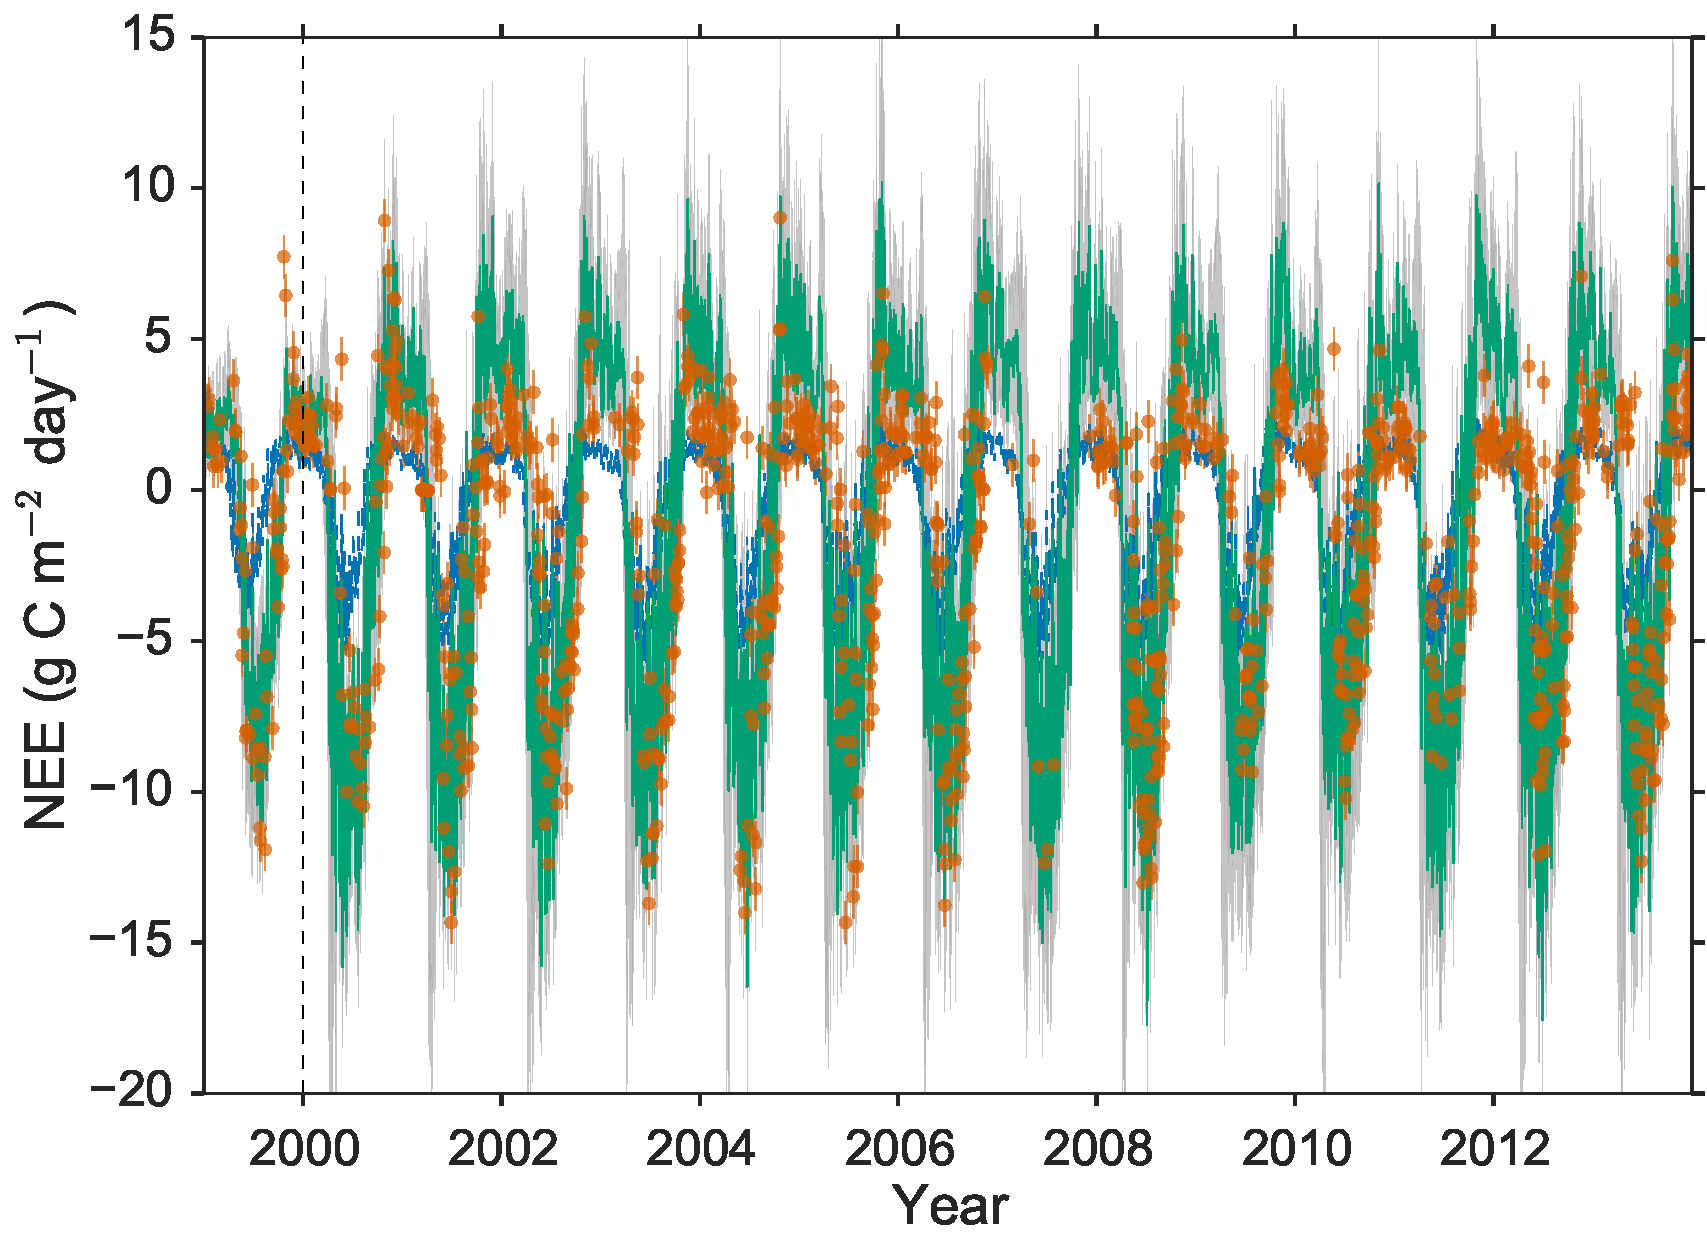
\includegraphics[width=\textwidth]{chapter/chapter6/A4dvar2.pdf}
        \caption{Experiment A}
        \label{fig:4dvardiagBR}
    \end{subfigure}
    \begin{subfigure}[b]{0.49\textwidth}
        \includegraphics[width=\textwidth]{chapter/chapter6/B4dvar2.pdf}
        \caption{Experiment B}
        \label{fig:4dvaredcBR}
    \end{subfigure}
    \begin{subfigure}[b]{0.49\textwidth}
        \includegraphics[width=\textwidth]{chapter/chapter6/C4dvar2.pdf}
        \caption{Experiment C}
        \label{fig:4dvarBcorR}
    \end{subfigure}
    \begin{subfigure}[b]{0.49\textwidth}
        \includegraphics[width=\textwidth]{chapter/chapter6/D4dvar2.pdf}
        \caption{Experiment D}
        \label{fig:4dvaredcBcorR}
    \end{subfigure}
    \caption{One year assimilation and fourteen year forecast of Alice Holt NEE with DALEC2, blue dotted line: background model trajectory, green line: analysis and forecast after assimilation, grey shading: Error in model after assimilation (+/- 3 standard deviations), red dots: observations from Alice Holt flux site with error bars.}\label{fig:4dvar}
\end{figure}

\begin{figure}
    \centering
    \begin{subfigure}[b]{0.49\textwidth}
        \includegraphics[width=\textwidth]{chapter/chapter6/Abroke4dvar2.pdf}
        \caption{Experiment A}
        \label{fig:broke4dvardiagBR}
    \end{subfigure}
    \begin{subfigure}[b]{0.49\textwidth}
        \includegraphics[width=\textwidth]{chapter/chapter6/Bbroke4dvar2.pdf}
        \caption{Experiment B}
        \label{fig:broke4dvaredcBR}
    \end{subfigure}
    \begin{subfigure}[b]{0.49\textwidth}
        \includegraphics[width=\textwidth]{chapter/chapter6/Cbroke4dvar2.pdf}
        \caption{Experiment C}
        \label{fig:broke4dvarBcorR}
    \end{subfigure}
    \begin{subfigure}[b]{0.49\textwidth}
        \includegraphics[width=\textwidth]{chapter/chapter6/Dbroke4dvar2.pdf}
        \caption{Experiment D}
        \label{fig:broke4dvaredcBcorR}
    \end{subfigure}
    \caption{As figure~\ref{fig:4dvar} but only showing the first and final two years results from the one year assimilation and fourteen year forecast of Alice Holt NEE with DALEC2, blue dotted line: background model trajectory, green line: analysis and forecast after assimilation, grey shading: Error in model after assimilation (+/- 3 standard deviations), red dots: observations from Alice Holt flux site with error bars.}\label{fig:broke4dvar}
\end{figure}

\begin{figure}
    \centering
    \begin{subfigure}[b]{0.49\textwidth}
        \includegraphics[width=\textwidth]{chapter/chapter6/Amoddat_resid.pdf}
        \caption{Experiment A}
        \label{fig:Amoddat_resid}
    \end{subfigure}
    \begin{subfigure}[b]{0.49\textwidth}
        \includegraphics[width=\textwidth]{chapter/chapter6/Bmoddat_resid.pdf}
        \caption{Experiment B}
        \label{fig:Bmoddat_resid}
    \end{subfigure}
    \begin{subfigure}[b]{0.49\textwidth}
        \includegraphics[width=\textwidth]{chapter/chapter6/Cmoddat_resid.pdf}
        \caption{Experiment C}
        \label{fig:Cmoddat_resid}
    \end{subfigure}
    \begin{subfigure}[b]{0.49\textwidth}
        \includegraphics[width=\textwidth]{chapter/chapter6/Dmoddat_resid.pdf}
        \caption{Experiment D}
        \label{fig:Dmoddat_resid}
    \end{subfigure}
    \caption{Net ecosystem exchange model-data differences for the four experiments. Here each point corresponds to the mean model-data difference for that day of the year over the 14 year model forecast (Jan 2000 - Dec 2013).}\label{fig:broke4dvar}
\end{figure}

\begin{figure}
    \centering
     \begin{subfigure}[b]{0.4\textwidth}
        \includegraphics[width=\textwidth]{chapter/chapter6/xbfscat2.pdf}
        \caption{Background}
        \label{fig:forecastscatxb}
    \end{subfigure}
    \begin{subfigure}[b]{0.4\textwidth}
        \includegraphics[width=\textwidth]{chapter/chapter6/Afscat2.pdf}
        \caption{Experiment A}
        \label{fig:forecastscatBR}
    \end{subfigure}
    \begin{subfigure}[b]{0.4\textwidth}
        \includegraphics[width=\textwidth]{chapter/chapter6/Bfscat2.pdf}
        \caption{Experiment B}
        \label{fig:forecastscatedcBR}
    \end{subfigure}
    \begin{subfigure}[b]{0.4\textwidth}
        \includegraphics[width=\textwidth]{chapter/chapter6/Cfscat2.pdf}
        \caption{Experiment C}
        \label{fig:forecastscatBcorR}
    \end{subfigure}
    \begin{subfigure}[b]{0.4\textwidth}
        \includegraphics[width=\textwidth]{chapter/chapter6/Dfscat2.pdf}
        \caption{Experiment D}
        \label{fig:forecastscatedcBcorR}
    \end{subfigure}
    \caption{Forecast scatter plot of modelled daily NEE vs. observations for Jan 2000 - Dec 2013 (green dots). Blue line represents the 1-1 line.}\label{fig:animals}
\end{figure}

\begin{figure}[ht]
    \centering
    \includegraphics[width=0.8\textwidth]{chapter/chapter6/inccvt2.pdf}
    \caption{Normalised analysis increment \big($\frac{(\textbf{x}^a - \textbf{x}^b)}{\textbf{x}^b}$\big) for the four experiments. Explanation of parameter and state variable symbols in table~\ref{table:xbvars}.}
    \label{fig:xa_inc}
\end{figure}

\subsection{Summary}

In our experiments we have shown that both $\textbf{B}_{corr}$ and $\hat{\textbf{R}}_{corr}$ have the effect of improving the model forecast of NEE. As it can be difficult to inspect the skill of a certain model by only plotting model trajectories, in figure~\ref{fig:taylordiag} we show Taylor diagrams displaying a statistical comparison of the four experiment and background analysis (Jan 1999 - Dec 1999) and forecast (Jan 2000 - Dec 2013) results with the observations of NEE. Here the radial distances from the origin to the points are proportional to the standard deviations of the observations and modelled observations and the azimuthal positions give the correlation coefficient between the modelled and observed NEE \citep{Taylor2001}. If a model predicted the observations perfectly it would have a correlation coefficient of $1$ and a radial distance matching that of the observations (represented by the dotted line). Figure~\ref{fig:td_a} shows that all the experiments give very similar results in the analysis window (Jan 1999 - Dec 1999) with all the experiment points closely grouped on top of each other, whereas figure~\ref{fig:td_f} shows the significant difference between the experiment results in the forecast (Jan 2000 - Dec 2013), with experiments B and D being closer to the dotted line. In all our experiments we find that $\theta_{min}$, $C_{lab}$ and $C_{fol}$ reach the bounds after assimilation. In the case of $\theta_{min}$ this is most likely due to the fact that we do not have enough information to recover this parameter when only assimilating observations of NEE, as the DALEC model prediction of NEE is insensitive to variations in this parameter \citep{Ann2013}. Assimilating more distinct data streams could help avoid this edge-hitting behaviour. For $C_{lab}$ and $C_{fol}$ this could suggest a flaw in the model or the fact that the prescribed bounds need to be relaxed slightly for the studied ecosystem. Our hypothesis is that the mechanism by which $C_{lab}$ is distributed to the leaves is over simplified; we intend to test this in future work. In table~\ref{table:expvars} we show the standard deviations for our parameter and state variables after assimilation. We can see that we have improved our confidence for most of these variables after assimilation when compared with the standard deviations in table~\ref{table:xbvars}.

\begin{figure}[ht]
    \centering
    \begin{subfigure}[b]{0.49\textwidth}
        \includegraphics[width=\textwidth]{chapter/chapter6/td.pdf}
        \caption{Analysis (Jan 1999 - Dec 1999)}
        \label{fig:td_a}
    \end{subfigure}
    \begin{subfigure}[b]{0.49\textwidth}
        \includegraphics[width=\textwidth]{chapter/chapter6/tdf.pdf}
        \caption{Forecast (Jan 2000 - Dec 2013)}
        \label{fig:td_f}
    \end{subfigure}
    \caption{Taylor diagrams displaying statistical comparison of the four experiment and background analysis (Jan 1999 - Dec 1999) and forecast (Jan 2000 - Dec 2013) results with observations of NEE $( \text{gCm}^{-2}\text{day}^{-1})$. The dotted line represents the standard deviation of the observations and the contours represent values of constant root mean square error between model and observations.}
    \label{fig:taylordiag}
\end{figure}

\begin{table}[ht] 
\begin{center}
	\begin{tabular}{| l | l | l | l |}
	\hline
	\multicolumn{4}{| c |}{Analysis (Jan 1999 - Dec 1999)} \\ \hline
	Experiment & RMSE $( \text{gCm}^{-2}\text{day}^{-1})$ & Bias $( \text{gCm}^{-2}\text{day}^{-1})$ & Correlation coefficient \\ \hline
	Background & $3.86$ & $-1.60$ & $0.70$ \\ \hline
	A & $1.36$ & $-0.03$ & $0.96$ \\ \hline
	B & $1.42$ & $-0.04$ & $0.95$ \\ \hline
	C & $1.37$ & $-0.09$ & $0.96$ \\ \hline
	D & $1.43$ & $-0.09$ & $0.95$ \\ \hline
	\multicolumn{4}{| c |}{Forecast (Jan 2000 - Dec 2013)} \\ \hline
	Experiment & RMSE $( \text{gCm}^{-2}\text{day}^{-1})$ & Bias $( \text{gCm}^{-2}\text{day}^{-1})$ &  Correlation coefficient \\ \hline
	Background & $3.86$ & $-1.36$ & $0.66$ \\ \hline
	A & $4.22$ & $-0.30$ & $0.79$ \\ \hline
	B & $2.56$ & $-0.20$ & $0.87$ \\ \hline
	C & $4.09$ & $-0.51$ & $0.78$ \\ \hline
	D & $2.38$ & $-0.33$ & $0.88$ \\ 
	\hline
	\end{tabular}
	\caption{Analysis (Jan 1999 - Dec 1999) and forecast (Jan 2000 - Dec 2013) results for experiments and background when judged against observed NEE.}
	\label{table:results}
\end{center} 
\end{table}


\section{Discussion}

In this paper we have implemented the DALEC2 functional ecology model in a 4D-Var data assimilation scheme, building an adjoint of the DALEC2 model and applying rigorous tests to our scheme. Using 4D-Var can provide much faster assimilation results than MCMC techniques as we have knowledge of the derivative of the model. For our experiments the 4D-Var routine has taken in the order of $10^{2}$ function evaluations to converge to a minimum, whereas MCMC techniques using the same model take in the order of $10^{8}$ function evaluations \citep{Bloom2015}. However, we do assume that the statistics of the problem are Gaussian whereas MCMC techniques do not. We have shown that 4D-Var is a valid tool for improving the DALEC2 model estimate of NEE and that even when assimilating only a single year of NEE observations we can improve the forecast significantly. If more than one year was required, this type of data assimilation routine could be run in cycling mode, allowing for the assimilation of multiple years of data \citep{moodycycled4dvar}. This also avoids any possible unstable behaviour associated with much longer single assimilation windows. However, here our aim is to investigate the effect of specifying correlations in background and observation error statistics on the forecast of NEE. We have therefore assimilated just one year of NEE observations and produced a long 14 year forecast in order to see more clearly the effect of including these correlations on the forecast when judging against observations. The observations of daily NEE from the Alice Holt flux site are quite variable year to year, peak summer uptake varies from $-14.35~\text{gCm}^{-2}\text{day}^{-1}$ to $-9.04~\text{gCm}^{-2}\text{day}^{-1}$, and therefore provide a reasonable test for the ability of the DALEC2 model forecast, especially over a 14 year period.  

We then considered the nature of background and observation errors. The effect of specifying parameter-state correlations in the background information and serial correlations between the observation errors was explored.

The technique presented here to specify ${\mathbf{B}}_{corr}$ has been shown to have significantly improved forecasts of NEE over using a diagonal representation of ${\mathbf{B}}$. In section~\ref{sec:expb} we discuss how the correlations in ${\mathbf{B}}_{corr}$ impact the analysis update for the parameter and state variables (see figure~\ref{fig:xa_inc}) causing the seasonal cycle of carbon uptake and magnitude of fluxes to fit more closely with the observations than when using a diagonal ${\mathbf{B}}$ in the assimilation algorithm. These results agree with those of \citet{smith2009variational} where the importance of specifying parameter-state correlations when performing joint parameter and state estimation with variational data assimilation was shown. The added constraint provided by including correlations in the prior error covariance matrix, $\textbf{B}$, acts to regularise the assimilation problem. Hence, the parameter and initial state values we retrieve from our data assimilation are more likely to be realistic, leading to better insight into the studied system. For example we see from figure~\ref{fig:xa_inc} that when using ${\mathbf{B}}_{corr}$ in our assimilation we find a much longer labile release period ($c_{ronset}$) than when using ${\mathbf{B}}_{diag}$. This means that the period of green-up in our study site is possibly much longer than we would have estimated had we based our analysis on our assimilation results using a matrix ${\mathbf{B}}$ with no correlations. The method for specifying ${\mathbf{B}}_{corr}$ in this paper used a series of ecological dynamical constraints taken from \citet{Bloom2015}. Implementing correlations in the prior error statistics in this way may prove difficult for models where these type of constraints are not available; however there are other methods to build correlations into $\textbf{B}$. One technique we also tested (not presented here) to create a correlated $\textbf{B}$ involved evolving an ensemble of state vectors over the length of the chosen assimilation window using the model (DALEC2) and then taking the covariance of the evolved ensemble. This gave us a \textbf{B} with parameter-state and state-state correlations, but no parameter-parameter correlations as the parameters are not updated by the model. Using the $\textbf{B}$ created with this method also improved assimilation results significantly over using a diagonal $\textbf{B}$. A larger number of different tests were run using different background vectors and variances and it was found that specifying some form of correlation structure in $\textbf{B}$ always made an improvement to the results of the assimilation. As this work has only considered a single deciduous site, it would be useful to apply the techniques detailed here for an evergreen site. Evergreen ecosystems usually have less extreme seasonal variation, it will therefore be of interest to see if a similar improvement for evergreen ecosystem forecast results is found when using a ${\mathbf{B}}_{corr}$ created using the same method.

The purpose of this exercise was to see how well we could forecast NEE while also investigating the effect of including correlations between error statistics. It was not an attempt to recover all the parameters and state variables with a high level of accuracy. However, it is still instructive to look at these values and compare with data where available. In \citet{meir2002acclimation} an observed range is given for leaf mass per area ($c_{lma}$) for the Alice Holt flux site of between $40$ to $80 ~\text{gCm}^{-2}$. The background value for $c_{lma}$ in our experiments is $128.5 ~\text{gCm}^{-2}$. When using diagonal error covariance matrices in experiment A we find a value of $38.7~\text{gCm}^{-2}$ for $c_{lma}$ after assimilation which is almost within the range given by \citet{meir2002acclimation}. In experiment D when using error covariance matrices including correlations $c_{lma}$ has a value of $51.6~\text{gCm}^{-2}$ after assimilation, this is well within the observed range given by \citet{meir2002acclimation}. From observations made by Forest Research we also have estimates of the above and below ground woody carbon pool ($C_{woo}$) at the start of 1999, with an observed value of $14258~\text{gCm}^{-2}$. It is not clear how uncertain this estimate is. The background value for $C_{woo}$ in our experiments is $6506~\text{gCm}^{-2}$. When using diagonal error covariance matrices in experiment A we find a value of $7291~\text{gCm}^{-2}$ for $C_{woo}$, an increase but still far away from the observed estimate. In experiment D when using error covariance matrices including correlations $C_{woo}$ has a value of $7262~\text{gCm}^{-2}$ a similar result as experiment A. Here the assimilation has not been able to recover a value of $C_{woo}$ similar to that of the observed estimate. This is not necessarily of concern as we are not able to quantify the error in this observation. Also we are assimilating observations of daily NEE only; NEE is the difference between Gross Primary Productivity (GPP) and Total ecosystem respiration (RT), (NEE = RT - GPP), with neither GPP nor RT being direct functions of $C_{woo}$. Therefore it is unlikely that we will recover an accurate value of $C_{woo}$, as the assimilated observations are not significantly impacted by large changes in this state variable; this result is also discussed in \citet{fox2009reflex}. This may also explains why we are able to recover a reasonable value of $c_{lma}$ from the assimilation, as from equation~\eqref{GPP} we can see that $c_{lma}$ is one of the input arguments taken by GPP. The function calculating NEE will therefore be sensitive to variations in the $c_{lma}$ parameter and so assimilating observations of NEE could help to constrain this parameter.

In numerical weather prediction it has been shown that including correlations in $\textbf{R}$ can help improve data assimilation results \citep{weston2014accounting, Stewart2013}. However the specified correlations have most commonly been satellite interchannel correlations with observations errors still being considered independent in time. In this paper we have shown that including correlations between observation errors in time can also improve data assimilation results, here providing a slight improvement for the DALEC2 model forecast of NEE. Here we only see a small impact on our results when using $\hat{\mathbf{R}}_{corr}$ in the assimilation as the correlations we have included are weak (especially in comparison to those included in ${\mathbf{B}}_{corr}$)  and on a short time-scale. We expect including correlations in $\hat{\textbf{R}}$ will have more of an impact on data assimilation results when assimilating data with stronger error correlations (i.e. finer temporal-resolution observations). We also expect including these serial correlations to have an even greater impact when assimilating more than one data stream as discussed in section~\ref{sec:intro}. Using the form of $\hat{\mathbf{R}}$ given in this paper for specifying serial correlations will also allow us to specify serial correlations between different observation types. When running the DALEC2 model with a day-night time step, instead of the daily time step used for this paper, this will allow us to build in the type of correlations investigated by \citet{Baldocchi2015} between ecosystem respiration and canopy photosynthesis. More work is needed to investigate the effect of including correlations between observations error statistics when assimilating multiple data streams.

The $\hat{\mathbf{R}}_{corr}$ presented in this paper has a weak correlation ($a=0.3$ as shown in section\ref{sec:corR}) in time between observations of NEE, this representation of $\hat{\mathbf{R}}_{corr}$ has slightly improved the model forecast of NEE. However other choices of $\hat{\mathbf{R}}_{corr}$ (with much stronger correlations between observations) tested for this paper degraded the forecast. This is probably due to the specified correlations being unrealistic and highlights the fact that a reasonable estimate of the true correlation structure for $\hat{\mathbf{R}}_{corr}$ is needed to have a positive impact on results. The development of a more diagnostic approach for the calculation of serial correlations in $\hat{\mathbf{R}}$ would be useful. One option would be to adapt the \citet{desroziers2005diagnosis} diagnostic, which has been used successfully in numerical weather prediction for diagnosing observation error correlations for observations taken at the same time \citep{weston2014accounting}, and extending this technique to diagnose serial correlations.

\section{Conclusion}

Functional ecology and land surface model data assimilation routines largely treat prior estimates of parameter and state uncertainties and observation error statistics as independent and uncorrelated. In this paper we have shown the importance of including estimates of such correlations, especially between background parameter and state error statistics when performing joint parameter and state estimation.

When performing joint parameter and state estimation including correlations in the background error covariance matrix significantly improves the forecast after assimilation, in comparison to using a diagonal representation of $\textbf{B}$. Specifying serial time correlations between observation errors in $\hat{\textbf{R}}$ also improves the forecast and we expect these correlations to have a greater impact when assimilating more than one data stream. More work is needed to investigate the effect of including these correlations when assimilating multiple data streams. The development of a more diagnostic tool for the calculation of the error correlation structure in $\hat{\textbf{R}}$ is also important.  

When including both parameter-state correlations in $\textbf{B}$ and time correlations between observation errors in $\hat{\textbf{R}}$ and assimilating only a single year of NEE observations we can forecast 14 years of NEE observations with a root-mean square error of $2.38~\text{gCm}^{-2}\text{day}^{-1}$ and a correlation coefficient of $0.88$. This is a significant $44\%$ reduction in error from the results when using a $\textbf{B}$ and $\hat{\textbf{R}}$ with no specified correlations of $4.22~\text{gCm}^{-2}\text{day}^{-1}$ and a correlation coefficient of $0.79$.

\section{Acknowledgements}

This work was funded by the UK Natural Environment Research Council (NE/K00705X/1) with a CASE award from the UK Forestry Commission. This work was also partly funded by the National Centre for Earth Observation. We are grateful to Luke Smallman for providing the data from the CARDAMOM system.

\newpage

\section{Appendix}

\begin{table}[ht] 
\begin{center}
	\begin{tabular}{| l | l | l | l | l |}
	\hline
	Parameter & Description & \pbox{7cm}{Background\\ vector ($\textbf{x}^{b}$)} & \pbox{7cm}{Standard \\deviation} & Range \\ \hline
$\theta_{min}$ & Litter mineralisation rate (day$^{-1}$) & $9.810\times 10^{-4}$ & $2.030\times 10^{-3}$ & $10^{-5} - 10^{-2}$ \\ \hline
$f_{auto}$ & Autotrophic respiration fraction & $5.190\times 10^{-1}$ & $1.168\times 10^{-1}$ & $0.3 - 0.7$  \\ \hline
$f_{fol}$ & Fraction of GPP allocated to foliage & $1.086\times 10^{-1}$ & $1.116\times 10^{-1}$ & $0.01-0.5$ \\ \hline
$f_{roo}$ & Fraction of GPP allocated to fine roots & $4.844\times 10^{-1}$ & $2.989\times 10^{-1}$ & $0.01-0.5$ \\ \hline
$c_{lspan}$ & Determines annual leaf loss fraction & $1.200\times 10^{0} $ & $1.161\times 10^{-1}$ & $1.0001 - 10$ \\ \hline
$\theta_{woo}$ & Woody carbon turnover rate (day$^{-1}$) & $1.013\times 10^{-4}$ & $1.365\times 10^{-4}$ & $2.5\times10^{-5} - 10^{-3}$ \\ \hline
$\theta_{roo}$ & Fine root carbon turnover rate (day$^{-1}$) & $3.225\times 10^{-3}$ & $2.930\times 10^{-3}$ & $10^{-4} - 10^{-2}$ \\ \hline
$\theta_{lit}$ & Litter carbon turnover rate (day$^{-1}$) & $3.442\times 10^{-3}$ & $3.117\times 10^{-3}$ & $10^{-4} - 10^{-2}$ \\ \hline
$\theta_{som}$ & Soil and organic carbon turnover rate (day$^{-1}$) & $1.113\times 10^{-4}$ & $1.181\times 10^{-4}$ & $10^{-7} - 10^{-3}$ \\ \hline
$\Theta$ & Temperature dependance exponent factor & $4.147\times 10^{-2}$ & $1.623\times 10^{-2}$ & $0.018 - 0.08$ \\ \hline
$c_{eff}$ & Canopy efficiency parameter & $7.144\times 10^{1}$ & $2.042\times 10^{1}$ & $10 - 100$ \\ \hline
$d_{onset}$ & Leaf onset day (day) & $1.158\times 10^{2}$ & $6.257\times 10^{0}$ & $1 - 365$ \\ \hline
$f_{lab}$ & Fraction of GPP allocated to labile carbon pool & $3.204\times 10^{-1}$ & $1.145\times 10^{-1}$ & $0.01 - 0.5$ \\ \hline
$c_{ronset}$ & Labile carbon release period (days) & $4.134\times 10^{1}$ & $1.405\times 10^{1}$ & $10 - 100$ \\ \hline
$d_{fall}$ & Leaf fall day (day) & $2.205\times 10^{2}$ & $3.724\times 10^{1}$ & $1 - 365$ \\ \hline
$c_{rfall}$ & Leaf-fall period (days) & $1.168\times 10^{2}$ & $2.259\times 10^{1}$ & $10 - 100$ \\ \hline
$c_{lma}$ & Leaf mass per area ($\text{gCm}^{-2}$) & $1.285\times 10^{2}$ & $6.410\times 10^{1}$ & $10 - 400$ \\ \hline
$C_{lab}$ & Labile carbon pool ($\text{gCm}^{-2}$) & $1.365\times 10^{2}$ & $6.626\times 10^{1}$ & $10 - 1000$ \\ \hline
$C_{fol}$ & Foliar carbon pool ($\text{gCm}^{-2}$) & $6.864\times 10^{1}$ & $3.590\times 10^{1}$ & $10 - 1000$ \\ \hline
$C_{roo}$ & Fine root carbon pool ($\text{gCm}^{-2}$) & $2.838\times 10^{2}$ & $2.193\times 10^{2}$ & $10 - 1000$ \\ \hline
$C_{woo}$ & Above and below ground woody carbon pool ($\text{gCm}^{-2}$) & $6.506\times 10^{3}$ & $7.143\times 10^{3}$ & $100 - 10^{5}$ \\ \hline
$C_{lit}$ & Litter carbon pool ($\text{gCm}^{-2}$) & $5.988\times 10^{2}$ & $5.450\times 10^{2}$ & $10 - 1000$ \\ \hline
$C_{som}$ & Soil and organic carbon pool ($\text{gCm}^{-2}$) & $1.936\times 10^{3}$ & $1.276\times 10^{3}$ & $100 - 2 \times 10^{5}$  \\ \hline
	\end{tabular}
	\caption{Parameter values and standard deviations for background vector used in experiments.}
	\label{table:xbvars}
\end{center} 
\end{table}

\begin{table}[ht] 
\begin{center}
	\begin{tabular}{| l | l | l | l | l |}
	\hline
	Parameter & A & B & C & D \\ \hline
$\theta_{min}$ & $1.822\times 10^{-6}$ & $3.742\times 10^{-7}$ & $1.519\times 10^{-6}$ & $3.854\times 10^{-7}$ \\ \hline
$f_{auto}$ & $2.913\times 10^{-3}$ & $1.428\times 10^{-3}$ & $2.937\times 10^{-3}$ & $1.510\times 10^{-3}$ \\ \hline
$f_{fol}$ & $5.459\times 10^{-3}$ & $4.581\times 10^{-3}$ & $6.797\times 10^{-3}$ & $4.591\times 10^{-3}$ \\ \hline
$f_{roo}$ & $7.907\times 10^{-2}$ & $9.141\times 10^{-3}$ & $8.199\times 10^{-2}$ & $9.149\times 10^{-3}$ \\ \hline
$c_{lspan}$ & $4.884\times 10^{-7}$ & $5.894\times 10^{-4}$ & $5.304\times 10^{-7}$ & $5.469\times 10^{-4}$ \\ \hline
$\theta_{woo}$ & $1.849\times 10^{-8}$ & $8.365\times 10^{-9}$ & $1.849\times 10^{-8}$ & $8.365\times 10^{-9}$ \\ \hline
$\theta_{roo}$ & $6.870\times 10^{-6}$ & $3.494\times 10^{-6}$ & $7.326\times 10^{-6}$ & $3.508\times 10^{-6}$ \\ \hline
$\theta_{lit}$ & $3.144\times 10^{-6}$ & $4.808\times 10^{-7}$ & $2.242\times 10^{-6}$ & $4.635\times 10^{-7}$ \\ \hline
$\theta_{som}$ & $1.178\times 10^{-8}$ & $6.848\times 10^{-9}$ & $1.210\times 10^{-8}$ & $6.850\times 10^{-9}$ \\ \hline
$\Theta$ & $7.905\times 10^{-5}$ & $6.808\times 10^{-5}$ & $8.010\times 10^{-5}$ & $6.978\times 10^{-5}$ \\ \hline
$c_{eff}$ & $3.755\times 10^{2}$ & $2.625\times 10^{2}$ & $3.724\times 10^{2}$ & $2.608\times 10^{2}$ \\ \hline
$d_{onset}$ & $3.552\times 10^{1}$ & $3.755\times 10^{1}$ & $3.649\times 10^{1}$ & $3.766\times 10^{1}$ \\ \hline
$f_{lab}$ & $1.220\times 10^{-2}$ & $3.209\times 10^{-3}$ & $1.225\times 10^{-2}$ & $3.203\times 10^{-3}$ \\ \hline
$c_{ronset}$ & $8.304\times 10^{1}$ & $1.642\times 10^{2}$ & $1.100\times 10^{2}$ & $1.644\times 10^{2}$ \\ \hline
$d_{fall}$ & $5.992\times 10^{2}$ & $5.294\times 10^{1}$ & $5.772\times 10^{2}$ & $6.145\times 10^{1}$ \\ \hline
$c_{rfall}$ & $1.540\times 10^{2}$ & $1.521\times 10^{2}$ & $1.604\times 10^{2}$ & $1.599\times 10^{2}$ \\ \hline
$c_{lma}$ & $2.134\times 10^{2}$ & $2.209\times 10^{2}$ & $2.503\times 10^{2}$ & $2.372\times 10^{2}$ \\ \hline
$C_{lab}$ & $6.142\times 10^{2}$ & $5.709\times 10^{2}$ & $8.586\times 10^{2}$ & $5.618\times 10^{2}$ \\ \hline
$C_{fol}$ & $7.971\times 10^{2}$ & $1.212\times 10^{2}$ & $8.029\times 10^{2}$ & $1.285\times 10^{2}$ \\ \hline
$C_{roo}$ & $3.984\times 10^{4}$ & $2.539\times 10^{4}$ & $4.114\times 10^{4}$ & $2.553\times 10^{4}$ \\ \hline
$C_{woo}$ & $5.075\times 10^{7}$ & $2.764\times 10^{7}$ & $5.075\times 10^{7}$ & $2.764\times 10^{7}$ \\ \hline
$C_{lit}$ & $4.157\times 10^{4}$ & $5.416\times 10^{4}$ & $7.179\times 10^{4}$ & $5.532\times 10^{4}$ \\ \hline
$C_{som}$ & $1.454\times 10^{6}$ & $1.106\times 10^{6}$ & $1.482\times 10^{6}$ & $1.105\times 10^{6}$  \\ \hline
	\end{tabular}
	\caption{Standard deviations for each experiment after assimilation, calculated using equation~\ref{eqn:Amat}.}
	\label{table:expvars}
\end{center} 
\end{table}


\chapter{Using data assimilation to understand the effect of disturbance on the carbon dynamics of the Alice Holt forest}
\label{chap:disturbance}
%Chapter 6

\section{Abstract}
The response of forests and terrestrial ecosystems to disturbance is an important process in the global carbon cycle in the context of a changing climate. In order to better understand ecosystem response to selective felling (thinning) in a managed forest site we use the mathematical technique of data assimilation to combine a diverse set of observations with a mathematical model of ecosystem carbon balance. We develop new data assimilation techniques allowing for the assimilation of daytime and nighttime net ecosystem exchange observations with a daily time-step model, increasing information available by a factor of 4.25. These techniques allow us to estimate the effect of step-changes in ecosystem composition on the parameter and state variables in a modelled estimate of forest carbon balance. These techniques are applicable to other ecosystem models and data assimilation schemes. 

Previous statistical analyses of eddy covariance data at the study site had suggested that disturbance from selective felling resulted in no significant change to the net carbon uptake of the ecosystem. Our results support this with a predicted net ecosystem carbon uptake for the year 2015 of \(426 \pm 116~\text{g C m}^{-2}\) for the unthinned forest and \(420 \pm 78~\text{g C m}^{-2}\) for the thinned forest despite a model-predicted reduction in gross primary productivity of \(337~\text{g C m}^{-2}\). We show that this is likely due to reduced ecosystem respiration post-disturbance compensating for a reduction in gross primary productivity. This supports the theory of an upper limit of forest net carbon uptake due to the magnitude of ecosystem respiration scaling with gross primary productivity. 


\section{Introduction}
%Disturbance can take many forms, for example; felling, fire and insect outbreak. In current estimates of the global carbon budget, disturbance is one of the least understood components. In this paper, we investigate the effect of the management practice f selective felling on the carbon dynamics of a mature temperate woodland.

%\subsection{\textcolor{red}{Role of disturbance in the global C cycle (make flow better?)}}
The response of forests and terrestrial ecosystems to disturbance (e.g. felling, fire, or insect outbreaks) is one of the least understood components in the global carbon cycle \citep{ciais2014carbon}. Current land surface models fail to represent the effect of disturbances on long-term carbon dynamics \citep{running2008ecosystem}, although these disturbances could have a significant effect on net land surface carbon uptake. Indeed, there could be significant variations in the effect as the range of forest disturbance can be wide: from stand replacing disturbance (where tree mortality is close to 100\%) to non-stand replacing disturbance, (where only a proportion of trees are lost). This paper uses data assimilation to improve the modelling of the non-stand replacing disturbance of selective felling (thinning) on forest carbon dynamics.

%\subsection{\textcolor{red}{Current theories on terrestrial ecosystem response to disturbance}}
Thinning is a silvicultural practice used to improve ecosystem services or the quality of a final tree crop and is globally widespread. The effect of thinning on carbon budgets has largely been ignored \citep{JGRG:JGRG779}. It would be intuitive to assume that after thinning we would see a reduction in the net carbon uptake of an ecosystem, due to reduced Gross Primary Productivity (GPP) following a reduction in total leaf area and unchanged or heightened ecosystem respiration due to an input of brash and woody debris to the forest floor. However, previous studies, analysing flux-tower eddy covariance records, find no significant change in the observed net ecosystem exchange (NEE) of CO\(_{2}\) after thinning \citep{vesala2005effect, moreaux2011paired,  dore2012recovery, Saunders20121, wilkinson2015effects}. These studies suggest this is due to increased light availability and reduced competition allowing ground vegetation to display increased GPP and compensate for an increase in heterotrophic respiration post-disturbance.  

Other studies have shown a significant reduction in the carbon content of rhizosphere soils following tree felling \citep{Hernesmaa2005777}. It has been shown that tree roots provide a rhizosphere priming effect, greatly increasing the rate of soil organic carbon decomposition \citep{ELE:ELE1095}, suggesting a decrease in respiration following thinning. This is consistent with previous work carried out at the study site in this paper, where it has been shown that the magnitude of ecosystem respiration is strongly coupled to the magnitude of GPP \citep{heinemeyer2012exploring}. Predictions made by \citet{kurz2008mountain} about the impacts of mountain pine beetle outbreaks in Northern American forests suggested a switch from sink to source of carbon following this disturbance. However, the analysis of a diverse set of observations for an area with approximately 70\% infested trees by \citet{ELE:ELE12097} revealed little change in net CO\(_{2}\) flux, due to concurrent reductions in GPP and ecosystem respiration. Similar results were also found from large scale tree girdling experiments \citep{hogberg2001large}, where 1-2 months after girdling a 54\% decrease in soil respiration was observed.

%\subsection{\textcolor{red}{The role of data assimilation for improving estimates to a system}}
Here we used data assimilation which is a mathematical technique for combining observations with prior model predictions in order to find the best estimate of a dynamical system. Functional ecology models have been combined with many different observations relevant to the carbon balance of forests \citep{Quaife2008, fox2009reflex, zobitz2011primer, richardson2010estimating, Zobitz2014, Niu2014, Pinnington2016299}, leading to improved estimates of model parameter and state variables and reduced uncertainty in model predictions. Although there have been many efforts to model the effect of disturbance on forest ecosystems \citep{thornton2002modeling, seidl2011modelling}, the use of data assimilation has been limited to a few examples, all of which used satellite data \citep{hilker2009new, kantzas2015improving}. The authors are not aware of any studies assimilating site level data to quantify disturbance effects. By assimilating observations relevant to post-disturbance ecosystem carbon dynamics with prior model predictions of ecosystem behaviour, we can analyse the retrieved parameters after data assimilation to find the model predicted effects of disturbance.   

%\subsection{\textcolor{red}{What does this paper do?}}
In this paper we investigate the effect of thinning on the carbon dynamics of the Alice Holt flux site \citep{wilkinson2012inter}, a deciduous managed woodland, following an event in 2014, when one side of the site was thinned and the other side left unmanaged. 
%During this thinning approximately 46\% of trees were removed from the studied area. In order to better understand the effect this thinning had on stand structure an intensive field campaign was undertaken in 2015 to measure leaf area index and also estimate woody biomass for both sides of the study site. The site has a flux tower positioned on the boundary between the thinned and unthinned forest. The eddy covariance record of NEE was split between the two sides using a flux footprint model. Previous statistical analysis of a thinning event in 2007 had suggested that there was no change in NEE between the thinned and unthinned sides of the forest post-disturbance \citep{wilkinson2015effects}.  
We present new methods for the assimilation of daytime and nighttime NEE observations with a daily time-step model, in this case the Data Assimilation Linked Ecosystem Carbon (DALEC2) model \citep{Bloom2015}. These methods require no model modification. We combine all available observations for 2015 with prior model predictions to find two sets of optimised model parameter and initial state values, corresponding to thinned and unthinned sides of the forest. We then use these two versions of the model to seek to explain why the net uptake of carbon remains unchanged even after removing a large proportion of the trees from one side. We find a net ecosystem carbon uptake for the year 2015 of \(426 \pm 116~\text{g C m}^{-2}\) for the unthinned forest and \(420 \pm 78~\text{g C m}^{-2}\) for the thinned forest, despite a reduction in GPP of \(337~\text{g C m}^{-2}\) for the thinned forest when compared to the unthinned forest. We find that reduced ecosystem respiration for the thinned forest allows for this unchanged net carbon uptake. The data assimilation techniques presented in this paper could be applied for similar analyses at other sites and provide a novel method to help elucidate the reasons behind ecosystem responses.      

\section{Observation and data assimilation methods}

\subsection{Alice Holt research forest} \label{sec:site_description}

Alice Holt Forest is a research forest area managed by the UK Forestry Commission located in Hampshire, SE England. Forest Research has been operating a $\text{CO}_{2}$ flux measurement tower in a portion of the forest, the Straits Inclosure, continuously since 1998. The Straits Inclosure is a $90~\text{ha}$ area of deciduous broadleaved plantation woodland located on a surface water gley soil and has been managed for the past 80 years. The majority of the canopy trees are oak (\textit{Quercus robur} L.), with an understory of hazel (\textit{Corylus avellana} L.) and hawthorn (\textit{Crataegus monogyna} Jacq.), but there is a small area of conifers (\textit{Pinus nigra} ssp. \textit{laricio} (Maire) and \textit{P. sylvestris} L.) within the tower measurement footprint area depending on wind direction. Further details of the Straits Inclosure site and the measurement procedures are given in \citet{wilkinson2012inter}, together with analysis of stand-scale $30$ minute average net $\text{CO}_{2}$ fluxes (NEE) from 1998-2011. 

As part of the management regime, the Straits Inclosure is subject to thinning, whereby a proportion of trees are removed from the canopy in order to reduce competition and improve the quality of the final tree crop. At the Straits an intermediate thinning method is used with a portion of both subdominant and dominant trees being removed from the stand \citep{kerr2011thinning}. The whole of the stand was thinned in 1995. Subsequently the eastern side of the Straits was thinned in 2007 and then the western side in 2014. The flux tower at the site is situated on the boundary between these two sides. This allows for the use of a footprint model to split the flux record and thus analyse the effect of this disturbance on carbon fluxes at the site. In \citet{wilkinson2015effects} a statistical analysis of the eddy covariance flux record found that there was no significant effect on the net carbon uptake of the eastern side after thinning in 2007. In this paper we focus on the effect of disturbance on the western side after thinning in 2014. We therefore refer to the western side as ``thinned'' forest and the eastern side as ``unthinned'' forest.   

\subsection{Observations} \label{sec:obs}

In order to assess the effect the 2014 thinning had on the Straits Inclosure, an intensive field campaign was undertaken in 2015 to measure leaf area index and also to estimate standing woody biomass. From the site we also have a long record of flux data, as discussed in section~\ref{sec:site_description}. These observations span both the thinned and unthinned sides of the forest.

\subsubsection{Leaf area index}

To assess the impact of the 2014 thinning, three transects were established in the Straits Inclosure for intensive sampling during 2015. A total of 435 sampling points were marked at 10~m apart, using a GPS and fluorescent tree spray paint. Measurements of peak LAI (July 2015 - September 2015) were made using both a ceptometer and hemispherical photography. The transects were walked twice with the ceptometer taking readings at every sampling point, giving 870 readings in total. Hemispherical photographs were taken every 50~m as shown in Figure~\ref{fig:hemi_lai}, giving 89 photographs in total. 

We measured below-canopy Photosynthetically Active Radiation (PAR) using the ceptometer while logging above-canopy PAR using a data logger and PAR sensor positioned outside the canopy. We then estimated LAI using the above-canopy and below-canopy PAR readings \citep{fassnacht1994comparison}. For the hemispherical photographs, we used the HemiView software \citep{rich1999hemiview} which calculates the proportion of visible sky as a function of sky direction (gap fraction) which it then uses to calculate LAI \citep{Jonckheere2004}.

Six litter traps were also established at points along the transects (positions shown in Figure~\ref{fig:hemi_lai}) allowing for comparison with the other methods. These were sampled throughout the leaf-fall season in 2015. We found the LAI derived from the litter traps was always greater than LAI estimated from optical methods, as expected \citep{breda2003ground}. From the sampling of the litter traps we also have estimates of leaf mass per area for use in data assimilation. As the 6 litter traps are not enough to describe the LAI for the research site \citep{kimmins1973some}, we used estimates from the ceptometer and hemispherical photographs for data assimilation. We took the weighted average (dependent on number of observations taken of each type) of the hemispherical photograph and ceptometer estimated LAI and derived an LAI of 4.42 with a standard error of 0.07 for the eastern unthinned forest, and an LAI of 3.06 with a standard error of 0.07 for the western thinned forest. We assimilated the mean of 299 LAI observations in the unthinned and 225 in the thinned section of forest. Consequently the appropriate representation of error for data assimilation is the standard error of the mean. From our litter trap observations we find a leaf mass per area of 29~g~C~m\(^{-2}\) free soluble carbohydrates for both sides of the forest.


\begin{figure}[ht]
    \centering
    \includegraphics[width=0.8\textwidth]{chapter/chapter7/thinned.pdf}
    \caption{LAI derived from hemispherical photographs for the Straits Inclosure at 50m intervals along three transects.} \label{fig:hemi_lai}
\end{figure}

\subsubsection{Woody biomass}  
The method of Point-Centred Quarters (PCQ) was used to conduct a biomass survey as specified in \citet{dahdouh2006empirical}. Along the three transects 114 points were sampled measuring the Diameter at Breast Height (DBH) and the density of trees. We then used allometric relationships between DBH and total above ground biomass and coarse root biomass, found in work carried out by Forest Research and in \citet{mckay2003woodfuel}, to find an estimate of total woody and coarse root carbon (referred to as \(C_{woo}\) in the DALEC2 model). These observations are shown in table~\ref{table:cwoo_obs}.

Forest Research have carried out their own mensuration studies at the site. One such study of the western thinned forest (at a similar time to our own PCQ measurements) found a tree density of 225 ha\(^{-1}\) and an average DBH of 32 cm, which are in close agreement to the estimates in table~\ref{table:cwoo_obs}. This gives us confidence that earlier measurements taken by Forest Research before the thinning are representative of the methods we have used. Measurements of the same section of forest from 2009 found a tree density of 418 ha\(^{-1}\) and an average DBH of 28 cm. This suggests that approximately 46\% of trees have been removed during the 2014 thinning. From these estimates we can also see the effect thinning has on the type of trees found at the site. The trees per hectare has dropped dramatically after thinning but the mean DBH has increased, because the smaller subdominant trees have been removed. The greater mean DBH of the eastern unthinned section, \(34~\text{cm}\), indicates that the thinning that took place in 2007 has allowed the dominant trees to grow as a result of reduced competition.

\begin{table}[ht] 
	\caption{Point-centred quarter method observations for 2015.}
\begin{center}
	\begin{tabular}{| l | p{2cm} | p{2cm} | p{4.5cm} |}
	\hline
	Sector & Tree density (ha\(^{-1}\)) & Mean DBH (cm) & Estimated woody biomass and coarse root carbon (g C m\(^{-2}\)) \\ \hline
	Unthinned (E) & 272 & 34.12 & 13130 \\ \hline
	Thinned (W) & 225 & 32.85 & 9908 \\ \hline
	\end{tabular}
	\label{table:cwoo_obs}
\end{center} 
\end{table}

\subsubsection{Flux tower eddy covariance} \label{sec:eddycov} 

The Straits Inclosure flux tower provides half-hourly observations from January 1999 to December 2015. These consist of the NEE fluxes and meteorological driving data of temperature, irradiance and atmospheric CO\(_{2}\) concentration for use in the DALEC2 model. The NEE data was subject to \(u^*\) filtering (with a value of \(0.2~\text{m s}^{-1}\)) and quality control procedures as described by \citet{papale2006towards}, but was not gap-filled. The resultant half-hourly NEE dataset was then split between observations corresponding to the western thinned and eastern unthinned sides of the site using a flux-footprint model, see \citet{wilkinson2015effects} for more details.  

To match the time-step of our model we computed daily NEE observations by taking the mean over the 48 measurements made each day, selecting only days where there is no missing data. As we have been strict on the quality control of the flux record and not used any gap filling, this presented a problem in terms of the number of daily NEE observations available. By further splitting the flux record between two sides we retrieved very few total daily observations of NEE for either side. In order to address this we computed day and nighttime NEE fluxes (NEE\(_{day}\) and NEE\(_{night}\) respectively) for use in data assimilation. We used a solar model to define whether NEE measurements were made at daytime or nighttime. We then took the mean over the half-hourly day or nighttime measurements, again only taking periods where there were no gaps in the data so that we were only considering true observations. This provided us with many more observations of NEE for assimilation, as seen in table~\ref{table:nee_obs}. Because we are averaging over shorter time periods we have a smaller probability of gaps and erroneous data. We see that we have more daytime NEE observations than nighttime, as we tend to have much more turbulent air mixing in daylight hours. In section~\ref{sec:da} we give details of how we relate these twice daily observations of NEE to a daily time-step model.     

\begin{table}[ht] 
	\caption{Number of observations of NEE, NEE\(_{day}\) and NEE\(_{night}\) for East and West sides of the Straits Inclosure for the year 2015.}
\begin{center}
	\begin{tabular}{| l | l | l | l | l |}
	\hline
	Sector & NEE & NEE\(_{day}\) & NEE\(_{night}\)  \\ \hline
	Unthinned (E) & 22 & 60 & 42 \\ \hline
	Thinned (W) & 26 & 54 & 48 \\ \hline
	\end{tabular}
	\label{table:nee_obs}
\end{center} 
\end{table}

The errors in observations of daily NEE were assumed to be constant and set at $0.5~\text{g C m}^{-2} \text{day}^{-1}$ by \citet{williams2005improved}, whereas \citet{braswell2005estimating} found these errors to be closer to $1~\text{g C m}^{-2} \text{day}^{-1}$. However, \citet{Richardson200838} show that flux errors are heteroscedastic. To account for the heteroscedastic nature of NEE errors we define an error function that scales between $0.5$ to $1~\text{g C m}^{-2} \text{day}^{-1}$ based on the magnitude of the observation. This function is defined as $0.5 + 0.04|\text{NEE}_{\text{day}}^{i}|~\text{g C m}^{-2} \text{day}^{-1}$, where \(|\text{NEE}_{\text{day}}^{i}|\) is the magnitude of the daytime NEE observation. \citet{raupach2005model} comment that nighttime measurements of NEE are much more uncertain than daytime measurements. This is difficult to quantify, but here we assume that nighttime flux errors are 3 times the magnitude of daytime errors. We therefore have the error function of $1.5 + 0.12|\text{NEE}_{\text{night}}^{i}|~\text{g C m}^{-2} \text{day}^{-1}$, where \(|\text{NEE}_{\text{night}}^{i}|\) is the magnitude of the nighttime NEE observation. We also include correlations in time between the errors in our observations of NEE, as discussed in \citet{Pinnington2016299}.

\subsection{Model and data assimilation}
\subsubsection{DALEC2 ecosystem carbon model} \label{sec:dalec2}

The DALEC2 model is a simple process-based model describing the carbon dynamics of a forest ecosystem \citep{Bloom2015}. The model is constructed of six carbon pools (labile ($C_{lab}$), foliage ($C_{fol}$), fine roots ($C_{roo}$), woody stems and coarse roots ($C_{woo}$), fresh leaf and fine root litter ($C_{lit}$) and soil organic matter and coarse woody debris ($C_{som}$)) linked via fluxes. The aggregated canopy model (ACM) \citep{williams1997predicting} is used to calculate daily gross primary production ($GPP$) of the forest, taking meteorological driving data and the modelled leaf area index (a function of $C_{fol}$) as arguments. Figure~\ref{fig:DALEC_mod} shows a schematic of how the carbon pools are linked in DALEC2; full model equations can be found in the appendix, section \ref{sec:dalec_eqns}.   

\begin{figure}[ht]
    \centering
    \includegraphics[width=0.6\textwidth]{chapter/chapter7/dalec2diag.pdf}
    \caption{Representation of the fluxes in the DALEC2 carbon balance model. Green arrows represent C allocation, purple arrows represent litter fall and decomposition fluxes, blue arrows represent respiration fluxes and the red arrow represents the influence of leaf area index in the $GPP$ function.} \label{fig:DALEC_mod}
\end{figure}

\subsubsection{Data assimilation} \label{sec:da}

We implement Four-Dimensional Variational data assimilation (4D-Var) with the DALEC2 model for joint parameter and state estimation \citep{navon1998practical}. In 4D-Var we aim to find the parameter and initial state values such that the model trajectory best fits the data over some time window, given some prior information about the system. This prior information takes the form of an initial estimate of the parameter and state variables of the model, $\textbf{x}^{b}$, valid at the initial time. This prior is assumed to have unbiased, Gaussian errors with known covariance matrix $\textbf{B}$. Adding the prior term ensures that our problem is well posed and that we can find a locally unique solution \citep{Tremolet2006}. We aim to find the parameter and initial state values that minimise the weighted squared distance to the prior and the weighted squared distance of the model trajectory to the observations, over a time window of length \(N\), with individual time points $t_{0}, \dots, t_{N}$. We do this by finding the state $\textbf{x}^{a}$ at time $t_{0}$ that minimises the cost function

\begin{equation}
J(\textbf{x}_0) = \frac{1}{2}(\textbf{x}_0-\textbf{x}^b)^{T}\textbf{B}^{-1}(\textbf{x}_0-\textbf{x}^b)+\frac{1}{2}\sum_{i=0}^{N}(\textbf{y}_i-\textbf{h}_i(\textbf{x}_i))^{T}\textbf{R}_{i}^{-1}(\textbf{y}_i-\textbf{h}_i(\textbf{x}_i)),
\end{equation}
where $\textbf{x}_{0}$ is the vector of parameter and initial state values to be optimised, $\textbf{x}_{i}$ is the vector of model variables at time \(t_{i}\), $\textbf{h}_{i}$ is the observation operator mapping the parameter and state values to the observations, $\textbf{y}_{i}$ is the vector of observations at time \(t_i\) and $\textbf{R}_{i}$ is the observation error covariance matrix. The time step, \(i\), is 1 day in this case. Further details of the implemented data assimilation scheme and specification of prior and observational errors can be found in \citet{Pinnington2016299}. 

In this paper we assimilate day and nighttime NEE in order to increase the number of observations available to us and also better partition our modelled estimate of GPP and total ecosystem respiration. As the DALEC2 model runs at a daily time step, this requires us to relate the daily parameter and state values from the model to the twice-daily observations of NEE. We do this by writing two new observation operators, one relating the model state and parameters to daytime NEE, and the other to nighttime NEE. The NEE of CO\(_{2}\) at any given time is the difference between GPP and ecosystem respiration. For an observation of total daily NEE on day \(i\) we have,
\begin{equation}
NEE^{i}=-GPP^{i}(C_{fol}^{i}, \Psi) +f_{auto}GPP^{i}(C_{fol}^{i}, \Psi) + \theta_{lit}C_{lit}^i e^{\Theta T^{i}} + \theta_{som}C_{som}^i e^{\Theta T^{i}}, \label{eqn: D1_nee}
\end{equation}
where \(\Psi\) represents meteorological driving data used the in the calculation of GPP, \(f_{auto}\) is the fraction of autotrophic respiration, \(\theta_{lit}\) is the litter carbon turnover rate, \(\theta_{som}\) is the soil and organic carbon turnover rate, \(\Theta\) is the temperature dependence exponent factor and \(T^{i}\) is the mean temperature over 24~hours. Further description can be found in the appendix section~\ref{sec:dalec_eqns}. The first term in equation~\eqref{eqn: D1_nee} represents gross primary productivity, the second autotrophic respiration and the third and fourth terms heterotrophic respiration. 

For total daytime NEE we have,
\begin{equation}
NEE_{day}^{i} = -GPP^{i}(C_{fol}^{i}, \Psi) + \delta_{day}f_{auto}GPP^{i}(C_{fol}^{i}, \Psi) + \delta_{day}\theta_{lit}C_{lit}^i e^{\Theta T_{day}^{i}} + \delta_{day}\theta_{som}C_{som}^i e^{\Theta T_{day}^{i}} \label{eqn: D1_nee_day}
\end{equation}
where \(\delta_{day}\) is \(\frac{\text{number of daylight hours}}{24}\), and \(T_{day}^{i}\) is the mean temperature over daylight hours. Here we still have the same term for GPP as in equation~\eqref{eqn: D1_nee} as all photosynthesis occurs during daylight hours. We have made the assumption that respiration is spread uniformly in time; therefore the respiration terms are scaled by the fraction of daylight hours. For nighttime NEE we have,
\begin{equation}
NEE_{night}^{i} =  \delta_{night}f_{auto}GPP^{i}(C_{fol}^{i}, \Psi) + \delta_{night}\theta_{lit}C_{lit}^i e^{\Theta T_{night}^{i}} + \delta_{night}\theta_{som}C_{som}^i e^{\Theta T_{night}^{i}} \label{eqn: D1_nee_night}
\end{equation}
where \(\delta_{night}\) is \(\frac{\text{number of night hours}}{24}\), and \(T_{night}^{i}\) is the mean nighttime temperature. In equation~\eqref{eqn: D1_nee} we do not have a term for GPP as no GPP will occur during the night. The respiration is here is scaled by the fraction of nighttime hours. The length of day and night are calculated using a solar model.

 These new observation operators allow for assimilation of day/nighttime NEE without the need for altering the model and can be applied to other ecosystem models to allow for the assimilation of eddy covariance data at a finer temporal resolution. 
%Cite MacBean?? for correlations?

\subsection{Experimental setup}
%Assimilation of 2015 years data post disturbance for the optimisation of two parameter sets, one corresponding to the unmanaged East and the other set to the managed West.

%In this paper we have split the flux tower eddy covariance record using a footprint model. This means we have observations of NEE for both the West and East sides of the forest stand. By combining these two distinct sets of observations with our prior model using 4D-Var data assimilation allows us to retrieve two unique sets of parameter and initial state values, .

In order to assess the information content of the three available data streams (described in section~\ref{sec:obs}) and their impact on the effect of disturbance as predicted by the model, we conducted a data denial procedure. This involved assimilating different combinations of observations, in three experiments, as shown in table~\ref{table:obs_da}. In our first experiment we used only the eddy covariance data, as this is the data type most commonly used in data assimilation studies. In the second we added the observations relating to leaf mass and area and finally in the third experiment we added the observations of woody biomass, as NEE observations have been shown to be unable to constrain this \citep{fox2009reflex}. In each experiment we used the prior model as specified in the appendix in table~\ref{table:xbvars}. This prior model was found by assimilating daytime and nighttime NEE, leaf mass per area and LAI observations from 2012 and 2013 before the thinning occurred. More information on the methods used to find this prior model can be found in \citet{Pinnington2016299}. 

%We ran three data assimilation experiments for the one year window of 2015. In these experiments we assimilated different combinations of observations as shown in table~\ref{table:obs_da}. By performing this type of ``data denial'' procedure we can assess the relative levels of information from the different data streams and their impact on the disturbance effect predicted by the model. In each experiment we used the prior model as specified in table~\ref{table:xbvars}. This prior model was found by assimilating daytime and nighttime NEE, leaf mass per area and LAI observations from 2012 and 2013 before the thinning occurred. More information on the methods used to find this prior model can be found in \citet{Pinnington2016299}.   

In each experiment we ran the assimilation for both the thinned forest and the unthinned forest, using the distinct data for each side. This allowed us to retrieve a unique set of parameter and initial state values for each section of forest. We analysed the optimised parameter and initial state values for the thinned and unthinned forest and also the model predictions of different variables for each side post-disturbance. This allowed us to judge the effect the thinning in 2014 had on the carbon dynamics of the forest in 2015.

\begin{table}[ht] 
	\caption{Combination of observations used in data assimilation experiments.}
\begin{center}
	\begin{tabular}{| l | l | l | l |}
	\hline
	Experiment & NEE & LAI \& leaf mass per area & C\(_{woo}\) \\ \hline
	A & \(\times\) &  &  \\ \hline
	B & \(\times\) & \(\times\) &  \\ \hline
	C & \(\times\) & \(\times\) & \(\times\)  \\ \hline
	\end{tabular}
	\label{table:obs_da}
\end{center} 
\end{table}

It would be expected that we will retrieve different estimates for each of the experiments outlined in table~\ref{table:obs_da}, with our most confident estimate being when all observations types are assimilated together in experiment C. This would allow us to see how much information each data stream provides and assess whether NEE data alone is enough to understand the effect of disturbance.

\section{Results} \label{sec:results}
%Show plots of East and West after assimilation and the change in optimised parameters. Confident in results as we know that even assimilating a single year of data we can accurately describe the carbon dynamics of the site for a long time period (15 years) into the future from Pinnington et al 2016.

In Figure~\ref{fig:obscompa} and \ref{fig:obscompc} we show the observations and model trajectories after assimilation for the  thinned and unthinned forest for experiments A and C respectively. We can see that the model fits all the assimilated observations well after assimilation for both experiments. We have confidence in our results as we have demonstrated previously that assimilating a single year of data can accurately forecast the carbon uptake of the site for a long time period (15 years) \citep{Pinnington2016299}. From Figure~\ref{fig:obscompa}a and \ref{fig:obscompa}b we see that the modified observation operators presented in section~\ref{sec:da} have allowed our model to represent both daytime and nighttime NEE well. 

In experiment A we have only assimilated NEE observations. From table~\ref{table:mod_rmse} we can see that we improve the fit to the assimilated observations for both the unthinned and thinned forest when compared to the prior model. The root-mean-square error (RMSE) is within the specified observation error for both daytime and nighttime NEE after assimilation. By only assimilating observations of NEE we have not been able to accurately predict LAI. Although we have improved the fit of the model to LAI after assimilation for the thinned forest (see table~\ref{table:mod_rmse}), we have significantly degraded the fit of the model to LAI for the unthinned forest. Partitioning the NEE dataset between the thinned and unthinned forest (as described in section~\ref{sec:eddycov}) has resulted in a gap in the observations for the unthinned forest during the period of greatest carbon uptake (June 2015 - August 2015), see Figure~\ref{fig:obscompa}a. This is due to the prevailing wind in this period being from the south-west. The gap in the NEE dataset when observations would have been of highest magnitude causes our model to under-predict the carbon uptake for the unthinned forest. This bias introduced into the NEE dataset for the unthinned forest results in a significantl under-prediction of LAI, as seen in Figure~\ref{fig:obscompa}c. From Figure~\ref{fig:obscompa}d and table~\ref{table:mod_rmse} we can see that NEE observations alone do not give us enough information to recover a value of \(C_{woo}\) with the DALEC2 model. This is also found in previous work \citep{fox2009reflex}.

In experiment B we have assimilated observations of NEE, LAI and leaf mass per area. From table~\ref{table:mod_rmse} we see that including the extra observations have allowed the model to fit LAI well for both the unthinned and thinned forest, and although the fit of the model to the NEE observations is slightly degraded, it is still well within the specified observation error from section~\ref{sec:eddycov}. We also see that including these extra observations still does not allow us to recover an accurate value of \(C_{woo}\).      

In experiment C we assimilate all available observations. This gives us very similar results as in experiment B, except that including the observations of \(C_{woo}\) in the assimilation allows the model to fit this observation well, as seen in table~\ref{table:mod_rmse}. We see from Figure~\ref{fig:obscompc}a and \ref{fig:obscompc}c that including observations of LAI in the assimilation removes the bias introduced from the partitioning of the NEE observations between the unthinned and thinned forest. The distinct difference in stand structure is now clear in Figure~\ref{fig:obscompc}, with reduced LAI and woody carbon for the thinned forest. For experiment C the time of senescence in LAI predicted by the model is consistent with phenocam observations made by Forest Research at the site, as shown in the supplementary material (Figure S12). However, the time of green-up in LAI predicted by the model is later than the phenocam observations. We hypothesise that this is due to the model predicting the photosynthetically effective LAI implicitly rather than the LAI related to canopy green index measured by the phenocam, which will show present LAI before new leaves become competent at photosynthesis \citep{reich1991leaf, Morecroft2003}.   

\begin{figure}[ht]
    \centering
        \includegraphics[width=\textwidth]{chapter/chapter7/obs_compa.pdf}
\caption{Experiment A: 2015 unthinned and thinned forest observations and model trajectories after assimilation. Blue line: model trajectory after assimilation of unthinned data, blue shading: uncertainty in model trajectory after assimilation (\(\pm\) 1 standard deviation), blue dots: unthinned observations with error bars, orange line: model trajectory after assimilation of thinned data, orange shading: uncertainty in model trajectory after assimilation (\(\pm\) 1 standard deviation), orange dots: thinned observations with error bars.}
 \label{fig:obscompa}
 \end{figure}
 
 \begin{figure}[ht]
    \centering
        \includegraphics[width=\textwidth]{chapter/chapter7/obs_compc.pdf}
\caption{Experiment C: 2015 unthinned and thinned forest observations and model trajectories after assimilation. Colour, lines and dots have the same meaning as described in Figure~\ref{fig:obscompa}. Figure c) and d) now also include observations of LAI and \(C_{woo}\) (dots).}
 \label{fig:obscompc}
 \end{figure}

\begin{table}[ht] 
	\caption{Root-mean-square error of model fit to observations for the prior model and all experiments after data assimilation.}
\begin{center}
	\begin{tabular}{| l | l | l | l | l | l}
	\hline
	\multicolumn{5}{| c |}{Unthinned forest} \\ \hline
	Exp. & NEE\(_{day}\) & NEE\(_{night}\)  & LAI & \(C_{woo}\)  \\ \hline
	Prior & 1.25 \(\text{g C m}^{-2}~\text{day}^{-1}\) & 1.02 \(\text{g C m}^{-2}~\text{day}^{-1}\)  & 0.43 & 5507 \(\text{g C m}^{-2}\)  \\ \hline
	A & 0.61 \(\text{g C m}^{-2}~\text{day}^{-1}\) & 0.83 \(\text{g C m}^{-2}~\text{day}^{-1}\)  & 2.16 & 6361 \(\text{g C m}^{-2}\)  \\ \hline
	B & 0.75 \(\text{g C m}^{-2}~\text{day}^{-1}\) & 0.93 \(\text{g C m}^{-2}~\text{day}^{-1}\) & 0.04 & 5987 \(\text{g C m}^{-2}\)  \\ \hline
	C & 0.75 \(\text{g C m}^{-2}~\text{day}^{-1}\) & 0.93 \(\text{g C m}^{-2}~\text{day}^{-1}\) & 0.04 & 0.16 \(\text{g C m}^{-2}\)  \\ \hline
	\multicolumn{5}{| c |}{Thinned forest} \\ \hline
	Exp. & NEE\(_{day}\) & NEE\(_{night}\)  & LAI & \(C_{woo}\)  \\ \hline
	Prior & 1.05 \(\text{g C m}^{-2}~\text{day}^{-1}\) & 0.61 \(\text{g C m}^{-2}~\text{day}^{-1}\) & 1.79 & 2285 \(\text{g C m}^{-2}\)  \\ \hline
	A & 0.63 \(\text{g C m}^{-2}~\text{day}^{-1}\) & 0.54 \(\text{g C m}^{-2}~\text{day}^{-1}\) & 0.55 & 2505 \(\text{g C m}^{-2}\)  \\ \hline
	B & 0.63 \(\text{g C m}^{-2}~\text{day}^{-1}\) & 0.56 \(\text{g C m}^{-2}~\text{day}^{-1}\) & 0.04 & 2241 \(\text{g C m}^{-2}\)  \\ \hline
	C & 0.63 \(\text{g C m}^{-2}~\text{day}^{-1}\) & 0.56 \(\text{g C m}^{-2}~\text{day}^{-1}\) & 0.04 & 0.07 \(\text{g C m}^{-2}\)  \\ \hline
	\end{tabular}
	\label{table:mod_rmse}
\end{center} 
\end{table}

Table~\ref{table:fluxes} shows the cumulative annual fluxes for the year 2015 for the three experiments. In all three experiments there is no significant difference between the net carbon uptake for the thinned and unthinned forest. We can see that both experiments B and C predict very similar cumulative fluxes, suggesting that the assimilated observations of \(C_{woo}\) have not had much impact on the model carbon dynamics for this time period. Because the rate parameters controlling this pool are relatively slow it is likely that observations of \(C_{woo}\) will become much more important over longer time-scales. Here we have only assimilated a single observation of \(C_{woo}\) for either side of the forest; if multiple observations of \(C_{woo}\) were available throughout time this would give us an estimate of the rate of woody biomass accumulation, providing an important constraint on the carbon assimilation of the forest. Experiments A and C both predict no significant difference in the net ecosystem carbon uptake between the thinned and unthinned forest. However, the partitioning of this carbon uptake between GPP and total ecosystem respiration (TER) is significantly different, with experiment A predicting increased TER and GPP after thinning and experiment C predicting reduced TER and GPP after thinning. This can be seen more clearly in Figure~\ref{fig:cum_flux}. The difference between the results of experiment A and C highlights the issue that NEE is the difference between two large fluxes (NEE = -GPP + TER) and we can therefore find an accurate prediction of NEE despite under/overestimating both GPP and TER. Therefore, care should be taken when interpreting model results based solely on NEE data, especially in this case, as we have seen that the partitioning of the NEE data between the thinned and unthinned forest has introduced a bias into our dataset. If we were to base our analysis on experiment A we would assume that the thinning had caused an increase in ecosystem respiration and that this had been compensated for by an increase in GPP. This is the opposite conclusion to the one we find in experiment C when we include observations relating to the structure of the forest. 

\begin{table}[ht] 
	\caption{Total annual fluxes and standard deviations for 2015 after assimilation \((\text{g C m}^{-2})\).}
\begin{center}
	\begin{tabular}{| l | l | l | l | l}
	\hline
	\multicolumn{4}{| c |}{Unthinned forest} \\ \hline
	Flux & Experiment A & Experiment B & Experiment C \\ \hline
	NEE & \(-379\pm 99\) & \(-425\pm113\) & \(-426\pm116\) \\ \hline
	GPP & \(1648\pm 159\) & \(2191\pm 87\) & \(2193\pm83\) \\ \hline
	TER & \(1267\pm 150\) & \(1766\pm146\) & \(1767\pm146\) \\ \hline
	\multicolumn{4}{| c |}{Thinned forest} \\ \hline
	Flux & Experiment A & Experiment B & Experiment C \\ \hline
	NEE & \(-394\pm 81\) & \(-421\pm73\) & \(-420\pm78\) \\ \hline
	GPP & \(1976\pm 112\) & \(1855\pm75\) & \(1856\pm80\) \\ \hline
	TER & \(1582\pm 134\) & \(1435\pm100\) & \(1436\pm109\) \\ \hline
	\end{tabular}
	\label{table:fluxes}
\end{center} 
\end{table}

\begin{figure}[ht]
    \centering
        \includegraphics[width=\textwidth]{chapter/chapter7/flux_part.pdf}
    \caption{Experiment A \& C: 2015 unthinned and thinned forest model trajectories for cumulative fluxes after assimilation. Solid line: cumulative NEE, dotted line: cumulative ecosystem respiration, dashed line: cumulative GPP. Colour and shading has the same meaning as in Figure~\ref{fig:obscompa}.} \label{fig:cum_flux}
\end{figure}


\begin{figure}[ht]
    \centering
        \includegraphics[width=\textwidth]{chapter/chapter7/resp_partc.pdf}
    \caption{Experiment C: 2015 unthinned and thinned forest model trajectory for cumulative total ecosystem respiration after assimilation and its partitioning between total autotrophic respiration and heterotrophic respiration from litter and soil.} \label{fig:rt_part}
\end{figure}

In Figure~\ref{fig:rt_part} we show the partitioning of cumulative ecosystem respiration for the year 2015 between total autotrophic respiration and heterotrophic respiration from litter and soil for both the unthinned and thinned forest in experiment C. Here we can see the strong dependance of autotrophic respiration on GPP with the growth rate being much greater between June 2015 - September 2015 (when GPP will be of greater magnitude). For heterotrophic respiration the growth rate is more constant throughout the whole year. Total ecosystem respiration is reduced by 331\(~\text{g C m}^{-2}\) for the thinned forest when compared to the unthinned forest, with reductions in both heterotrophic and autotrophic respiration of 169\(~\text{g C m}^{-2}\) and 162\(~\text{g C m}^{-2}\) respectively.    

\begin{figure}[ht]
    \centering
    \includegraphics[width=0.8\textwidth]{chapter/chapter7/xa_incc.pdf}
    \caption{Experiment C: normalised change in parameter and state variables after data assimilation \big($\frac{(\textbf{x}^a(j) - \textbf{x}^b(j))}{\textbf{x}^b(j)}$\big) for the unthinned and thinned forest. Explanation of parameter and state variable symbols in table~\ref{table:xbvars}.}
    \label{fig:xa_inc}
\end{figure}

Figure~\ref{fig:xa_inc} shows the change in parameter and initial state values for the thinned and unthinned forest after assimilating all observations in experiment C. It is important to note that this is the difference when compared to our prior model estimate, which was found by assimilating only eddy covariance, LAI and leaf mass per area observations from 2012 and 2013. We therefore expect changes in parameter and state values for both the thinned and unthinned forest, as we are assimilating new data streams. This is particularly noticeable in the carbon pool state variables in Figure~\ref{fig:xa_inc}. Constraints on the carbon pool state variables are provided by the assimilated observations of woody biomass and coarse roots (\(C_{woo}\)), LAI and leaf mass per area (\(c_{lma}\)). LAI and \(c_{lma}\) give us a constraint on foliar carbon (\(C_{fol}\)) as LAI \(= \frac{C_{fol}}{c_{lma}} \). We can see the values for the model predicted carbon pools are as we might expect with the thinned forest having less carbon in all pools when compared to the unthinned forest. For litter carbon (\(C_{lit}\)) we expect a reduction in input of leaf litter for the thinned forest and, although there might be increased woody debris after thinning, this is much less readily decomposed and so possibly has little impact in the year after thinning \citep{wilkinson2016}. The difference in predicted soil carbon content (\(C_{som}\)) between the thinned and unthinned forest is consistent with studies analysing soil carbon contents after felling \citep{Hernesmaa2005777}. For the parameters the biggest changes appear to be in the litter carbon turnover rate parameter (\(\theta_{lit}\)), with the retrieved parameter being significantly reduced for the unthinned forest when compared to the thinned. However, we still see reduced total litter respiration in Figure~\ref{fig:rt_part} for the thinned forest compared to the unthinned forest. This is due to the significant difference in litter carbon content (\(C_{lit}\)) for both sides, with the unthinned forest having a much higher litter carbon content than the thinned forest. The large change in the \(\theta_{lit}\) parameter between the two sides is therefore compensating for an overestimated difference in litter carbon content between the two sides.    
 \clearpage
 
 
\section{Discussion}
In this paper we have used data assimilation to combine observations and prior model predictions of ecosystem carbon balance in order to understand how the state of an ecosystem might be altered after a disturbance event. We conducted three experiments assimilating different combinations of available data streams. For all experiments we find no significant change in net carbon uptake for the studied ecosystem following stand thinning, where approximately 46\% of trees were removed. This is consistent with other studies of ecosystem carbon dynamics following thinning. We find different reasons for this unchanged carbon uptake dependent on which data streams are assimilated. When only assimilating NEE observations we find increased ecosystem respiration and increased GPP post-disturbance. These results are unreliable due to bias introduced into the NEE dataset from partitioning between the thinned and unthinned forest. From our most confident estimate, where all available observations are assimilated, the model shows that reductions in GPP, following a decrease in total leaf area post-thinning, are being offset by simultaneous reductions in ecosystem respiration. This is in contrast to current suggestions that reduced canopy photosynthesis is compensated for by increased GPP by ground vegetation post-thinning \citep{vesala2005effect, moreaux2011paired, dore2012recovery, wilkinson2016}.

%however does support work investigating the effect of insect disturbance \citep{ELE:ELE12097}.

Our results show a decrease in both autotrophic and heterotrophic respirations following thinning. Autotrophic respiration has both above and below ground components, whereas heterotrophic respiration is mainly from soils and litter. We follow the definition of \citet{heinemeyer2012exploring} and characterise below ground autotrophic respiration as respiration from roots, mycorrhizal fungi and other micro-organisms dependent on the priming of soils with labile carbon compounds from roots. It has been shown recently that deep root systems and their influences may be more widespread than previously thought \citep{Pierret01102016}. Heterotrophic respiration is respiration by microbes not directly dependent on autotrophic substrate; however, the largest fraction of heterotrophic respiration is based on the decomposition of young organic matter (e.g. leaves and fine roots) whose availability also depends on the GPP of an ecosystem \citep{GCB:GCB412}. We find similar decreases in both heterotrophic and autotrophic respiration for the thinned forest when compared with the unthinned forest. While it has been shown that heterotrophic respiration can decrease after disturbance events \citep{PCE:PCE1053}, it is possible we overestimate the reduction in heterotrophic respiration and underestimate the reduction in autotrophic respiration. This is understandable as we have assimilated no data on this partitioning. Also our model description of autotrophic respiration is simple (described as a constant fraction of GPP) and therefore the heterotrophic respiration component of the model might compensate and in this instance describe the behaviour of mycorrhizal fungi and other microbes commonly categorised in the autotrophic component of respiration.   

In a study measuring soil CO\(_{2}\) fluxes over 4 years at the Straits Inclosure (the study site in this paper) \citet{heinemeyer2012exploring} showed a large 56\% contribution of autotrophic respiration (characterised as root and mycorrhizal respiration) to total measured soil respiration. \citet{heinemeyer2012exploring} also suggested that mycorrhizal fungi play a role in priming the turnover of soil organic carbon by other microbes, with evidence from \citet{talbot2008decomposers}. \citet{hogberg2006towards} find similar figures for the autotrophic contribution to total soil respiration, with around half or more of all soil respiration being driven by recent photosynthesis. \citet{heinemeyer2012exploring} discuss the possibility of this tight coupling between GPP and ecosystem respiration leading to an upper limit for forest CO\(_{2}\) uptake due to increased GPP leading to increased respiration, which is also discussed by \citet{heath2005rising}. Our results support this hypothesis, as ecosystem respiration scales with GPP after approximately 46\% of trees are removed from the study site, meaning that we find no significant change in net ecosystem carbon uptake after thinning.   

Studies analysing eddy covariance flux records also find no significant change in the net ecosystem exchange of CO\(_{2}\) after thinning \citep{vesala2005effect, moreaux2011paired, dore2012recovery, wilkinson2016}. These studies hypothesise that the unchanged NEE is due to increased GPP by ground vegetation (following increased light availability and reduced competition) compensating for increases in heterotrophic respiration and reduced canopy photosynthesis post-thinning. We do not find evidence to support such hypothesis and instead suggest that reduced ecosystem respiration is the most important component for the unchanged NEE of the forest following thinning. However, it is important to note that our measurements of LAI are made at approximately 1~m above the forest floor, which means that our measurements of LAI do not account for ground vegetation. Therefore, any effect of this ground vegetation is not simulated by our model. Despite this, observations made during multiple walks of the three established transects find no evidence of increased ground vegetation in the year after thinning. In fact much of the ground vegetation and subcanopy was removed during thinning and did not appear to have recovered in the following year. At longer time-scales re-growth of the subcanopy and ground vegetation will play an important role in increased productivity. Our results suggest that this increased productivity would also be met with subsequent increases in ecosystem respiration.

%Para about reduction in respiration being logical. Partition been auto hetero could be ``wrong''

%\citep{Pierret01102016} also been shown recently that deep root systems may be more widespread than previously thought.

%\citep{hogberg2006towards} half of all soil respiration driven by recent photosynthesis.

%\citep{PCE:PCE1053} heterotrophic respiration decreased 1 to 2 years post-disturbance in girdling experiments due to reduced fine root input as respiratory substrate.

%\citep{heinemeyer2012exploring} shows at same study site that GPP and autotrophic substrate main driver for ecosystem respiration.

The effect of disturbance is poorly characterised in current land surface and global climate models \citep{running2008ecosystem}; it is important to better understand how parameters and carbon pools might change following disturbance. DALEC2 and many other ecosystem models assume that respiration rates are proportional to carbon pool size. It has been suggested that although this assumption works well in equilibrium conditions it may not allow such models to predict ecosystem carbon dynamics following disturbance \citep{schimel2003implications}. The data assimilation techniques in this paper present a way for these simple models to cope with step changes in ecosystem behaviour, by allowing parameters and carbon pools to be updated following disturbance events. 


%From the assimilation of multiple data streams with a model of ecosystem carbon balance we find evidence that reduced heterotrophic respiration following disturbance allows a managed woodland to exhibit an unchanged net carbon uptake when compared against an undisturbed section of the same woodland. 

\section{Conclusion}

In this work we have presented novel methods for understanding ecosystem responses to disturbance by using data assimilation. Assimilating all available data streams after an event of disturbance with a prior model prediction allows us to assess changes to model parameter and state variables due to this disturbance. We have also created modified observation operators to allow for the assimilation of daytime and nighttime NEE observations with a daily time-step model. This negated the need for model modification and increased the number of observations by a factor of 4.25.

Our modelled estimates show no significant change in net ecosystem carbon uptake after a thinning event in 2014 where approximately 46\% of trees were removed from the studied area. Similar results were also found following a thinning activity in 2007 \citep{wilkinson2016}. From our optimised model we find that reduced ecosystem respiration is the main reason for this unchanged net ecosystem carbon uptake. Therefore, even for a decrease in GPP following thinning, there is no significant change in NEE. We hypothesise this reduction in ecosystem respiration is due to reduced input of autotrophic substrate following thinning, meaning both autotrophic and heterotrophic respiration are reduced. These results support work suggesting that GPP is the dominant driver for ecosystem respiration  \citep{GCB:GCB412, PCE:PCE1053, hogberg2006towards, heinemeyer2012exploring, ELE:ELE12097}. This has implications for future predictions of land surface carbon uptake and whether forests will continue to sequester atmospheric CO\(_{2}\) at similar rates, or if they will be limited by increased GPP leading to increased respiration. 

\section{acknowledgments}
This work was funded by the UK Natural Environment Research Council (NE/K00705X/1) with a CASE award from the UK Forestry Commission. This work was also partly funded by the National Centre for Earth Observation. We are grateful to Ian Craig for providing Forest Research mensuration estimates.

Code and data available at: https://github.com/dalec-reading/4dvar\_dalec\_alice\_holt

\section{Appendix} \label{sec:appendix}

\subsection{DALEC2 equations} \label{sec:dalec_eqns}

The model equations for the carbon pools at day $i$ are as follows:

\begin{align}
GPP^{i} &= ACM(C_{fol}^{i-1}, c_{lma}, c_{eff}, \Psi) \label{GPP}
\\C_{lab}^{i}&=C_{lab}^{i-1}+(1-f_{auto})(1-f_{fol})f_{lab}GPP^{i}-\Phi _{on}C_{lab}^{i-1}, \label{daleclab}
\\C_{fol}^{i}&=C_{fol}^{i-1}+\Phi_{on}C_{lab}^{i-1}+(1-f_{auto})f_{fol}GPP^{i}-\Phi_{off}C_{fol}^{i-1}, \label{dalec1}
\\C_{roo}^{i}&=C_{roo}^{i-1}+(1-f_{auto})(1-f_{fol})(1-f_{lab})f_{roo}GPP^{i}-\theta_{roo}C_{roo}^{i-1}, 
\\C_{woo}^{i}&=C_{woo}^{i-1}+(1-f_{auto})(1-f_{fol})(1-f_{lab})(1-f_{roo})GPP^{i}-\theta_{woo}C_{woo}^{i-1}, 
\\C_{lit}^{i}&=C_{lit}^{i-1}+\theta_{roo}C_{roo}^{i-1}+\Phi_{off}C_{fol}^{i-1}-(\theta_{lit}+\theta_{min})e^{\Theta T^{i-1}}C_{lit}^{i-1}, 
\\C_{som}^{i}&=C_{som}^{i-1}+\theta_{woo}C_{woo}^{i-1}+\theta_{min}e^{\Theta T^{i-1}}C_{lit}^{i-1}-\theta_{som}e^{\Theta T^{i-1}}C_{som}^{i-1}, \label{dalec5}
\end{align}
where $T^{i-1}$ is the daily mean temperature, $\Psi$ represents the meteorological driving data used in the $GPP$ function and $\Phi_{on} / \Phi_{off}$ are functions controlling leaf-on and leaf-off. Descriptions for each model parameter used in equations \eqref{GPP} to \eqref{dalec5} are included in table~\ref{table:xbvars}. DALEC2 can be parameterised for both deciduous and evergreen sites with $\Phi_{on}$ and $\Phi_{off}$ being able to reproduce the phenology of either type of site. The full details of this version of DALEC can be found in \cite{Bloom2015}. 

\begin{table}[ht] 
	\caption{Parameter values and standard deviations for prior vector used in experiments.}
\begin{center}
\scriptsize
	\begin{tabular}{| l | p{4.5cm} | p{1.7cm} | p{1.7cm} | p{1.7cm} |}
	\hline
	Parameter & Description & Prior estimate ($\textbf{x}^{b}$) & Standard deviation & Range \\ \hline
$\theta_{min}$ & Litter mineralisation rate (day$^{-1}$) & $5.471\times 10^{-4}$ & $6.828\times 10^{-7}$ & $10^{-5} - 10^{-2}$ \\ \hline
$f_{auto}$ & Autotrophic respiration fraction & $4.492\times 10^{-1}$ & $1.814\times 10^{-4}$ & $0.3 - 0.7$  \\ \hline
$f_{fol}$ & Fraction of GPP allocated to foliage & $4.091\times 10^{-2}$ & $1.211\times 10^{-4}$ & $0.01-0.5$ \\ \hline
$f_{roo}$ & Fraction of GPP allocated to fine roots & $3.700\times 10^{-1}$ & $3.389\times 10^{-3}$ & $0.01-0.5$ \\ \hline
$c_{lspan}$ & Determines annual leaf loss fraction & $1.089\times 10^{0} $ & $2.777\times 10^{-3}$ & $1.0001 - 10$ \\ \hline
$\theta_{woo}$ & Woody carbon turnover rate (day$^{-1}$) & $1.012\times 10^{-4}$ & $3.040\times 10^{-9}$ & $2.5\times10^{-5} - 10^{-3}$ \\ \hline
$\theta_{roo}$ & Fine root carbon turnover rate (day$^{-1}$) & $5.411\times 10^{-3}$ & $1.353\times 10^{-6}$ & $10^{-4} - 10^{-2}$ \\ \hline
$\theta_{lit}$ & Litter carbon turnover rate (day$^{-1}$) & $4.387\times 10^{-3}$ & $1.825\times 10^{-6}$ & $10^{-4} - 10^{-2}$ \\ \hline
$\theta_{som}$ & Soil and organic carbon turnover rate (day$^{-1}$) & $1.311\times 10^{-4}$ & $2.705\times 10^{-9}$ & $10^{-7} - 10^{-3}$ \\ \hline
$\Theta$ & Temperature dependance exponent factor & $9.354\times 10^{-2}$ & $6.810\times 10^{-5}$ & $0.018 - 0.08$ \\ \hline
$c_{eff}$ & Canopy efficiency parameter & $5.618\times 10^{1}$ & $6.676\times 10^{0}$ & $10 - 100$ \\ \hline
$d_{onset}$ & Leaf onset day (day) & $1.584\times 10^{2}$ & $1.370\times 10^{1}$ & $1 - 365$ \\ \hline
$f_{lab}$ & Fraction of GPP allocated to labile carbon pool & $7.927\times 10^{-2}$ & $1.491\times 10^{-4}$ & $0.01 - 0.5$ \\ \hline
$c_{ronset}$ & Labile carbon release period (days) & $1.891\times 10^{1}$ & $6.011\times 10^{1}$ & $10 - 100$ \\ \hline
$d_{fall}$ & Leaf fall day (day) & $3.049\times 10^{2}$ & $1.046\times 10^{2}$ & $1 - 365$ \\ \hline
$c_{rfall}$ & Leaf-fall period (days) & $5.447\times 10^{1}$ & $1.502\times 10^{2}$ & $10 - 100$ \\ \hline
$c_{lma}$ & Leaf mass per area ($\text{g C m}^{-2}$) & $2.929\times 10^{1}$ & $7.099\times 10^{2}$ & $10 - 400$ \\ \hline
$C_{lab}$ & Labile carbon pool ($\text{g C m}^{-2}$) & $7.309\times 10^{1}$ & $1.672\times 10^{3}$ & $10 - 1000$ \\ \hline
$C_{fol}$ & Foliar carbon pool ($\text{g C m}^{-2}$) & $1.313\times 10^{1}$ & $6.707\times 10^{2}$ & $10 - 1000$ \\ \hline
$C_{roo}$ & Fine root carbon pool ($\text{g C m}^{-2}$) & $2.103\times 10^{2}$ & $2.024\times 10^{4}$ & $10 - 1000$ \\ \hline
$C_{woo}$ & Above and below ground woody carbon pool ($\text{gCm}^{-2}$) & $7.182\times 10^{3}$ & $2.019\times 10^{7}$ & $100 - 10^{5}$ \\ \hline
$C_{lit}$ & Litter carbon pool ($\text{g C m}^{-2}$) & $1.697\times 10^{2}$ & $4.958\times 10^{4}$ & $10 - 1000$ \\ \hline
$C_{som}$ & Soil and organic carbon pool ($\text{g C m}^{-2}$) & $1.950\times 10^{3}$ & $8.344\times 10^{5}$ & $100 - 2 \times 10^{5}$  \\ \hline
	\end{tabular}
	\label{table:xbvars}
\end{center} 
\end{table}


\section{Supplementary material}

%Type or paste your text here. The introduction gives a brief overview of the supporting information. You should include information %about as many of the following as possible (when appropriate):
% 1. a general overview of the kind of data files;
% 2. information about when and how the data were collected or created;
% 3. a general description of processing steps used;
% 4. any known imperfections or anomalies in the data.

In Figures~\ref{fig:fluxcompa}-\ref{fig:fluxcumd} we present extra plots from the three experiments outlined in the paper (A, B \& C). We also add plots for a fourth experiment (labelled experiment D here) where only LAI, leaf mass per area and woody biomass are assimilated with the DALEC2 model. The summary statistics for experiment D are also included in table~\ref{table:sum_stats}.

In Figure~\ref{fig:prior_mod} we show the prior model trajectory and observations of daytime NEE for 2012-2013. This is the period in which the prior model was calibrated.

Figure~\ref{fig:pheno_obs} shows phenocam observations of green fraction taken at the Alice Holt flux site. The LAI as predicted by experiment C is also shown on this figure.

 
\begin{figure}
 \noindent\includegraphics[width=40pc]{chapter/chapter7/flux_compa.pdf}
\caption{Experiment A: 2015 unthinned and thinned forest model trajectories after assimilation. Blue line: model trajectory after assimilation of unthinned forest data, blue shading: uncertainty in model trajectory after assimilation (\(\pm\) 1 standard deviation), orange line: model trajectory after assimilation of thinned forest data, orange shading: uncertainty in model trajectory after assimilation (\(\pm\) 1 standard deviation).}
 \label{fig:fluxcompa}
 \end{figure}
 
 \begin{figure}
 \noindent\includegraphics[width=40pc]{chapter/chapter7/cum_fluxa.pdf}
\caption{Experiment A: 2015 unthinned and thinned forest model trajectories for cumulative fluxes after assimilation. Solid line cumulative NEE, dotted line: cumulative ecosystem respiration, dashed line: cumulative GPP (NEE=-GPP+RT). Colour and shading has the same meaning as in Figure~\ref{fig:fluxcompa}.}
 \label{fig:fluxcuma}
 \end{figure}


 \begin{figure}
 \noindent\includegraphics[width=40pc]{chapter/chapter7/obs_compb.pdf}
\caption{Experiment B: 2015 unthinned and thinned forest observations and model trajectories after assimilation. Blue line: model trajectory after assimilation of unthinned data, blue shading: uncertainty in model trajectory after assimilation (\(\pm\) 1 standard deviation), blue dots: unthinned observations with error bars, orange line: model trajectory after assimilation of thinned data, orange shading: uncertainty in model trajectory after assimilation (\(\pm\) 1 standard deviation), orange dots: thinned observations with error bars.}
 \label{fig:obscompb}
 \end{figure}
 
 
 \begin{figure}
 \noindent\includegraphics[width=40pc]{chapter/chapter7/flux_compb.pdf}
\caption{Experiment B: 2015 unthinned and thinned forest model trajectories after assimilation. Colour and shading has the same meaning as in Figure~\ref{fig:fluxcompa}.}
 \label{fig:fluxcompb}
 \end{figure}
 
  \begin{figure}
 \noindent\includegraphics[width=40pc]{chapter/chapter7/cum_fluxb.pdf}
\caption{Experiment B: 2015 unthinned and thinned forest model trajectories for cumulative fluxes after assimilation. Solid line cumulative NEE, dotted line: cumulative ecosystem respiration, dashed line: cumulative GPP (NEE=-GPP+RT). Colour and shading has the same meaning as in Figure~\ref{fig:fluxcompa}.}
 \label{fig:fluxcumb}
 \end{figure}
 
  \begin{figure}
 \noindent\includegraphics[width=40pc]{chapter/chapter7/flux_compc.pdf}
\caption{Experiment C: 2015 unthinned and thinned forest model trajectories after assimilation. Colour and shading has the same meaning as in Figure~\ref{fig:fluxcompa}.}
 \label{fig:fluxcompc}
 \end{figure}
 
  \begin{figure}
 \noindent\includegraphics[width=40pc]{chapter/chapter7/cum_fluxc.pdf}
\caption{Experiment C: 2015 unthinned and thinned forest model trajectories for cumulative fluxes after assimilation. Solid line cumulative NEE, dotted line: cumulative ecosystem respiration, dashed line: cumulative GPP (NEE=-GPP+RT). Colour and shading has the same meaning as in Figure~\ref{fig:fluxcompa}.}
 \label{fig:fluxcumc}
 \end{figure}
 
 
  \begin{figure}
 \noindent\includegraphics[width=40pc]{chapter/chapter7/obs_compd.pdf}
\caption{Experiment D: 2015 unthinned and thinned forest observations and model trajectories after assimilation. Blue line: model trajectory after assimilation of unthinned data, blue shading: uncertainty in model trajectory after assimilation (\(\pm\) 1 standard deviation), blue dots: unthinned observations with error bars, orange line: model trajectory after assimilation of thinned data, orange shading: uncertainty in model trajectory after assimilation (\(\pm\) 1 standard deviation), orange dots: thinned observations with error bars.}
 \label{fig:obscompd}
 \end{figure}
 
 
 \begin{figure}
 \noindent\includegraphics[width=40pc]{chapter/chapter7/flux_compd.pdf}
\caption{Experiment D: 2015 unthinned and thinned forest model trajectories after assimilation. Colour and shading has the same meaning as in Figure~\ref{fig:fluxcompa}.}
 \label{fig:fluxcompd}
 \end{figure}
 
  \begin{figure}
 \noindent\includegraphics[width=40pc]{chapter/chapter7/cum_fluxd.pdf}
\caption{Experiment D: 2015 unthinned and thinned forest model trajectories for cumulative fluxes after assimilation. Solid line cumulative NEE, dotted line: cumulative ecosystem respiration, dashed line: cumulative GPP (NEE=-GPP+RT). Colour and shading has the same meaning as in Figure~\ref{fig:fluxcompa}.}
 \label{fig:fluxcumd}
 \end{figure}
 
 
 \begin{figure}[ht]
 \noindent\includegraphics[width=40pc]{chapter/chapter7/prior.pdf}
    \caption{Prior model prediction and observations of daytime NEE for 2012-2013. Green line: model predicted value, orange dots: observations with error bars. The prior model has a correlation coefficient of 0.96 in this case.} 
    \label{fig:prior_mod}
\end{figure}


\begin{figure}[ht]
 \noindent\includegraphics[width=40pc]{chapter/chapter7/pheno_lai.pdf}
    \caption{Model predicted LAI for experiment C and Alice Holt phenocam observations of green fraction (green dots), calculated for the canopy region of interest using red-green-blue digital numbers for each pixel, see \citet{mizunuma2013relationship} for more details.} \label{fig:pheno_obs}
\end{figure}


\begin{figure}[ht]
 \noindent\includegraphics[width=30pc]{chapter/chapter7/rmat_eastc.pdf}
    \caption{Observation error correlation matrix for thinned forest used in experiment C data assimilation. For more details see \citet{Pinnington2016299}.} \label{fig:rmat_ut}
\end{figure}


\begin{figure}[ht]
 \noindent\includegraphics[width=30pc]{chapter/chapter7/rmat_westc.pdf}
    \caption{Observation error correlation matrix for unthinned forest used in experiment C data assimilation. For more details see \citet{Pinnington2016299}.} \label{fig:rmat_t}
\end{figure}
% ---------------
% EXAMPLE TABLE
%
\begin{table}[ht] 
	\caption{Fit to observations after data assimilation for experiments.}
\begin{center}
	\begin{tabular}{| l | l | l | l | l | l | l | l}
	\hline
	\multicolumn{7}{| c |}{Unthinned side} \\ \hline
	& \multicolumn{2}{| c |}{NEE\(_{day}\)} & \multicolumn{2}{| c |}{NEE\(_{night}\)} & LAI & \(C_{woo}\) \\ \hline
	Exp. & RMSE & \(r^2\) & RMSE & \(r^2\) & RMSE & RMSE  \\ \hline
	A & 0.61 & 0.97 & 0.83 & 0.31 & 2.16 & 6361  \\ \hline
	B & 0.75 & 0.90 & 0.93 & 0.64 & 0.04 & 5987  \\ \hline
	C & 0.75 & 0.90 & 0.93 & 0.64 & 0.04 & 0.16  \\ \hline
	D & 1.22 & 0.74 & 1.00 & 0.89 & 0.0004 & 0.19  \\ \hline
	\multicolumn{7}{| c |}{Thinned side} \\ \hline
	& \multicolumn{2}{| c |}{NEE\(_{day}\)} & \multicolumn{2}{| c |}{NEE\(_{night}\)} & LAI & \(C_{woo}\) \\ \hline
	Exp. & RMSE & \(r^2\) & RMSE & \(r^2\) & RMSE & RMSE  \\ \hline
	A & 0.63 & 0.97 & 0.54 & 0.33 & 0.55 & 2505  \\ \hline
	B & 0.63 & 0.97 & 0.56 & 0.27 & 0.04 & 2241  \\ \hline
	C & 0.63 & 0.97 & 0.56 & 0.27 & 0.04 & 0.07  \\ \hline
	D & 1.24 & 0.88 & 0.60 & 0.17 & 0.001 & 0.07  \\ \hline
	\end{tabular}
	\label{table:sum_stats}
\end{center} 
\end{table}



%more chapters...

\chapter{Conclusion}
\label{chap:conclusion}
%Chapter 1

This thesis has explored data assimilation for the terrestrial carbon cycle. The state of the global carbon cycle in the IPCC AR5 suggests that the land surface is the most uncertain component of the global carbon cycle. The response of ecosystem carbon uptake to land use change and disturbance (e.g. fire, felling, insect outbreak) is a large component of this uncertainty. The uncertainties in land surface carbon cycling processes are largely due to gaps in direct observations and poor parameterisations of model processes. Data assimilation provides methods to improve current estimates by combining observations with prior model estimates. In order to improve data assimilation results it is important that we add the most possible information about a system to data assimilation schemes. The equates to large amounts and more accurate information in, equals better information out. This could mean new observations with high levels of information for constraining poorly understood processes, or better characterisation of prior model and observational errors. Both the optimal set of observations and appropriate representation of error in data assimilation for the carbon cycle are not well understood. Based on this and knowledge of other components of uncertainty three key areas of research were identified in chapter~\ref{chap:intro}:
\begin{enumerate}
\item \textit{Investigating the information content in distinct carbon balance observations for data assimilation}

\item \textit{Improving the representation of prior and observational errors in carbon cycle data assimilation}

\item \textit{Using data assimilation to understand the effect of disturbance on forest carbon dynamics}
\end{enumerate}
The following sections will address these points in turn based on the work presented in this thesis in chapter~\ref{chap:info_con}--\ref{chap:disturbance}.

\section{Investigating the information content in distinct carbon balance observations for data assimilation}

In chapter~\ref{chap:info_con} we used both the DALEC1 and DALEC2 models of ecosystem carbon balance in a series of information content experiments. We calculated the tangent linear model of DALEC1 analytically by hand so that we could make novel applications of information content metrics relying on the adjoint of the model code. For the more complex and nonlinear DALEC2 joint state and parameter estimation case the tangent linear model was calculated using automatic differentiation. From the information content experiments in this chapter we deduced the following conclusions:
\begin{itemize}
\item For both the DALEC1 and DALEC2 models we found our system was observable for the available observations of NEE. This means that for data assimilation we can construct a locally unique solution from observational information alone. This is important as it give us confidence in subsequent experimental results relying on NEE as the main source for observational information.
\item There was a strong temporal variation in information content for observations of NEE, with observations made at times of higher temperatures having higher information content. For deciduous ecosystems observations of NEE made at times of leaf-on and leaf-off have higher influence in the assimilation as these act to help constrain the phenology of the model. 
\item Including an increasing correlation between NEE observation errors in time reduced the information content in the assimilated observations. 
\item It was clear from these experiments that in order to further improve understanding of the information content in observations it is important to improve estimates and representations of uncertainty for both prior model predictions and observations.
\end{itemize}

\section{Improving the representation of prior and observational errors in carbon cycle data assimilation}

In chapter~\ref{chap:error_corrs} we implemented and tested a 4D-Var data assimilation scheme with the DALEC2 model. We then used this system to investigate the effect of including correlations between prior model and NEE observation errors. In each experiment we assimilated a single year of NEE observations (1999) and then ran a 14 year forecast (2000-2014) of NEE. From this work our conclusions were:
\begin{itemize}
\item Including correlations in the background error covariance matrix significantly improved the model forecast after assimilation. Correlations in the observation error covariance matrix between NEE observation errors in time had much less of an effect on results. However, we expect these correlations will have more impact when assimilating more than one data stream or assimilating observations of NEE at a finer temporal resolution.
\item When correlations were included in both the background error covariance matrix and the observation error covariance matrix we found the best model forecast results. In this case the forecast root-mean-square error was reduced by a significant $44\% $ in comparison to when a diagonal background and observation error covariance matrix were used in assimilation.
\end{itemize} 


\section{Using data assimilation to understand the effect of disturbance on forest carbon dynamics}

In chapter~\ref{chap:disturbance} we again utilised the 4D-Var data assimilation scheme with DALEC2 outlined in chapter~\ref{chap:error_corrs} along with a set of observations taken on a fieldwork campaign to investigate the effect of selective felling on the carbon dynamics of the Alice Holt forest. We conducted a data-denial experiments using all the available observations to understand their effect on the modelled predicted effect of disturbance. We also propose novel observation operators allowing for the assimilation of daytime and nighttime NEE observations with a daily time-step model. The main results in this chapter were as follows:
\begin{itemize}
\item The proposed observation operators allow our model to accurately predict daytime and nighttime NEE and negate the need for any model modification. 
\item We find no change to the net ecosystem carbon uptake after felling when approximately 46\% of trees were removed from the area of interest.
\item Our most confident modelled estimate (when all available data is assimilated) suggests this unchanged carbon uptake is due to GPP being the main driver for both autotrophic and heterotrophic respiration, so that even with reduced GPP post-disturbance the same NEE can occur due to significant reductions in total ecosystem respiration. We find different conclusions if we base our conclusions solely on the assimilation of NEE observations, highlighting the need for caution not to over-interpret results when assimilating only this variable. 
\end{itemize}

\section{Future work}

The continued application of information content measures is important to better understand where to base efforts in future observation campaigns. It is also important to improve estimates of uncertainty for both prior model predictions and observations. This will ensure that results from information content experiments can be as accurate as possible. It would also be interesting to use a more complex model of ecosystem carbon dynamics where we could judge the impact of more novel measurements such as stem respiration.

We have shown that including a more sophisticated representation of error in data assimilation schemes can be of great benefit to results. more work in this area is important to improve the representation of uncertainty in data assimilation schemes. In relation to the experiments carried out in this thesis its is clear that a more diagnostic tool for the specification of observation error correlations is important. One possibility for this would be to use a method such as the \citet{desroziers2005diagnosis} diagnostic to statistically estimate the error covariance structure of assimilated observations. In order to diagnose correlations in time (similar to those specified in chapter~\ref{chap:error_corrs}) the \citet{desroziers2005diagnosis} diagnostic would have to be expanded. The \citet{desroziers2005diagnosis} diagnostic estimates the observation error covariance matrix as
\begin{equation}
\textbf{R} = \mathbb{E}[(\textbf{y}-\textbf{h}(\textbf{x}_a))(\textbf{y}-\textbf{h}(\textbf{x}_b))^{T}]
\end{equation}
this could be re-written as
\begin{equation}
\hat{\textbf{R}} = \mathbb{E}[(\hat{\textbf{y}}-\hat{\textbf{h}}(\textbf{x}_a))(\hat{\textbf{y}}-\hat{\textbf{h}}(\textbf{x}_b))^{T}]
\end{equation}
to estimate time correlations in the observation error covariance matrix. This would require that an ensemble of 4D-Var data assimilations were run with perturbed prior model estimates and perturbed observations. We could then retrieve a statistical estimate of the temporal correlation structure for the observation error covariance matrix. It will also be useful to test these new covariance matrices with included correlations at other research sites and with larger model implementations.

The results we find for the effect of disturbance are possibly surprising however do support ecological measurement campaigns analysing soil microbial communities after selective felling events. This experiment would be good to carry out again after collecting a few more years of data to understand the recovery of leaf area and long term response of the Alice Holt forest to disturbance. If possible it would be extremely beneficial to also set up soil respiration chambers on both the thinned and unthinned sides of the forest to improve constraint on the constituent processes.

\newpage
\addcontentsline{toc}{chapter}{Bibliography}
\def\rightmark{Bibliography}
\def\leftmark{Bibliography}
\renewcommand*{\bibname}{\centerline{\Huge{\bfseries{\scshape{Bibliography}}}}}
\bibliography{../PhD}
%\bibliography{chapter/chapter2/chapter2refs,chapter/chapter3/chapter3refs,chapter/chapter4/chapter4refs,chapter/chapter5/chapter5refs}
\bibliographystyle{./ametsoc}

\end{document}
